%-------------------------------------------------------------------------------
% This file provides a skeleton ATLAS document.
%-------------------------------------------------------------------------------
% \pdfoutput=1
% The \pdfoutput command is needed by arXiv/JHEP/JINST to ensure use of pdflatex.
% It should be included in the first 5 lines of the file.
%-------------------------------------------------------------------------------
% Specify where ATLAS LaTeX style files can be found.
\newcommand*{\ATLASLATEXPATH}{latex/}
% Use this variant if the files are in a central location, e.g. $HOME/texmf.
% \newcommand*{\ATLASLATEXPATH}{}
%-------------------------------------------------------------------------------
\documentclass[UKenglish,texlive=2013]{\ATLASLATEXPATH atlasdoc}
% The language of the document must be set: usually UKenglish or USenglish.
% british and american also work!
% Commonly used options:
%  texlive=YYYY          Specify TeX Live version (2013 is default).
%  atlasstyle=true|false Use ATLAS style for document (default).
%  coverpage             Create ATLAS draft cover page for collaboration circulation.
%                        See atlas-draft-cover.tex for a list of variables that should be defined.
%  cernpreprint          Create front page for a CERN preprint.
%                        See atlas-preprint-cover.tex for a list of variables that should be defined.
%  PAPER                 The document is an ATLAS paper (draft).
%  CONF                  The document is a CONF note (draft).
%  PUB                   The document is a PUB note (draft).
%  BOOK                  The document is of book form, like an LOI or TDR (draft)
%  txfonts=true|false    Use txfonts rather than the default newtx - needed for arXiv submission.
%  paper=a4|letter       Set paper size to A4 (default) or letter.

%-------------------------------------------------------------------------------
% Extra packages:
\usepackage{\ATLASLATEXPATH atlaspackage}
% Commonly used options:
%  biblatex=true|false   Use biblatex (default) or bibtex for the bibliography.
%  backend=biber         Use the biber backend rather than bibtex.
%  subfigure|subfig|subcaption  to use one of these packages for figures in figures.
%  minimal               Minimal set of packages.
%  default               Standard set of packages.
%  full                  Full set of packages.
%-------------------------------------------------------------------------------
% Style file with biblatex options for ATLAS documents.
\usepackage{\ATLASLATEXPATH atlasbiblatex}

% Package for creating list of authors and contributors to the analysis.
\usepackage{\ATLASLATEXPATH atlascontribute}

% Useful macros
\usepackage{\ATLASLATEXPATH atlasphysics}
% See doc/atlas_physics.pdf for a list of the defined symbols.
% Default options are:
%   true:  journal, misc, particle, unit, xref
%   false: BSM, heppparticle, hepprocess, hion, jetetmiss, math, process, other, texmf
% See the package for details on the options.

% Files with references for use with biblatex.
% Note that biber gives an error if it finds empty bib files.
%\addbibresource{atlas-document.bib}
\usepackage{gbb_int-defs}
\addbibresource{bibtex/bib/ATLAS.bib}
\addbibresource{int.bib}

% Paths for figures - do not forget the / at the end of the directory name.
\graphicspath{{logos/}{figures/}}

% Add you own definitions here (file atlas-document-defs.sty).
%\usepackage{atlas-document-defs}


%-------------------------------------------------------------------------------
% Some new shortcuts
%-------------------------------------------------------------------------------
%\def\dPMETsecondLargeRjet{\ensuremath{ \Delta\phi(\Ptmiss,2^{\text{nd}} \text{large-R jet})}}


\newcommand\drbb{{ \ensuremath{\Delta R(b_1, b_2)} }}
\newcommand\mll{{ \ensuremath{m(\ell^+,\ell^-)} }}
\newcommand\ptll{{ \ensuremath{p_T(\ell^+,\ell^-)} }}
\newcommand\mbl{{ \ensuremath{m(b,\ell)} }}
\newcommand\mmmbl{{ \text{min-max}\ \mbl }}


%-------------------------------------------------------------------------------
% Generic document information
%-------------------------------------------------------------------------------

% Title, abstract and document 
%-------------------------------------------------------------------------------
% This file contains the title, author and abstract.
% It also contains all relevant document numbers used by the different cover pages.
%-------------------------------------------------------------------------------

% Title
\AtlasTitle{Measuring the properties of $g\rightarrow b\bar{b}$ at small opening angles in $pp$ collisions with the ATLAS detector at $\sqrt{s}=13$ TeV}

% Author - this does not work with revtex (add it after \begin{document})
%\author{The ATLAS Collaboration}

% Authors and list of contributors to the analysis
% \AtlasAuthorContributor also adds the name to the author list
% Include package latex/atlascontribute to use this
% Use authblk package if there are multiple authors, which is included by latex/atlascontribute
% \usepackage{authblk}
% Use the following 3 lines to have all institutes on one line
% \makeatletter
% \renewcommand\AB@affilsepx{, \protect\Affilfont}
% \makeatother
% \renewcommand\Authands{, } % avoid ``. and'' for last author
% \renewcommand\Affilfont{\itshape\small} % affiliation formatting
 \AtlasAuthorContributor{Zihao Jiang}{a}{Main analyzer}
 \AtlasAuthorContributor{Benjamin Nachman}{b}{Truth studies, unfolding code, writing, advising}
 \AtlasAuthorContributor{Lauren Tompkins}{a}{Comments}
% \AtlasAuthorContributor{Michael Kagan}{c}{Comments}
% \AtlasContributor{Fourth AtlasContributor}{Contribution to the analysis.}
% \author[a]{First Author}
% \author[a]{Second Author}
% \author[b]{Third Author}
 \affil[a]{Stanford University, USA}
  \affil[b]{Lawrence Berkeley National Laboratory, USA}
 % \affil[c]{SLAC National Laboratory, USA}       

% If a special author list should be indicated via a link use the following code:
% Include the two lines below if you do not use atlasstyle:
% \usepackage[marginal,hang]{footmisc}
% \setlength{\footnotemargin}{0.5em}
% Use the following lines in all cases:
% \usepackage{authblk}
% \author{The ATLAS Collaboration%
% \thanks{The full author list can be found at:\newline
%   \url{https://atlas.web.cern.ch/Atlas/PUBNOTES/ATL-PHYS-PUB-2016-007/authorlist.pdf}}
% }

% Draft version:
% Should be 1.0 for the first circulation, and 2.0 for the second circulation.
% If given, adds draft version on front page, a 'DRAFT' box on top of each other page, 
% and line numbers.
% Comment or remove in final version.
\AtlasVersion{0.8}

% ATLAS reference code, to help ATLAS members to locate the paper
\AtlasRefCode{STDM-2017-17}

% ATLAS note number. Can be an COM, INT, PUB or CONF note
% \AtlasNote{ATLAS-CONF-2016-XXX}
% \AtlasNote{ATL-PHYS-PUB-2016-XXX}
% \AtlasNote{ATL-COM-PHYS-2016-XXX}

% CERN preprint number
% \PreprintIdNumber{CERN-PH-2016-XX}

% ATLAS date - arXiv submission; usually filled in by the Physics Office
% \AtlasDate{\today}

% ATLAS heading - heading at top of title page. Set for TDR etc.
% \AtlasHeading{ATLAS ABC TDR}

% arXiv identifier
% \arXivId{14XX.YYYY}

% HepData record
% \HepDataRecord{ZZZZZZZZ}

% Submission journal and final reference
% \AtlasJournal{Phys.\ Lett.\ B.}
% \AtlasJournalRef{\PLB 789 (2014) 123}
% \AtlasDOI{}

% Abstract - % directly after { is important for correct indentation
\AtlasAbstract{%
The fragmentation of high energy gluons at small opening angles is largely unconstrained with present measurements.  Gluon splitting to $b$-quark pairs is a unique probe into the properties of gluon fragmentation because identified $b$-tagged jets provide a proxy for the quark daughters of the initial gluon.  This note documents the measurement of key differential distributions related to $g\rightarrow b\bar{b}$ using the 2016 dataset.  Track jets are used to probe angular scales below the standard $R=0.4$ jet radius.  The observables are unfolded to particle level in order to facilitate direct comparison with predictions from present and future simulations. These data will provide an important constraint to hadronization models that is particularlly relevant for boosted Higgs analyses where the main background results from gluon splitting to b-quarks.
}

%-------------------------------------------------------------------------------
% The following information is needed for the cover page. The commands are only defined
% if you use the coverpage option in atlasdoc or use the atlascover package
%-------------------------------------------------------------------------------

% List of supporting notes  (leave as null \AtlasCoverSupportingNote{} if you want to skip this option)
% \AtlasCoverSupportingNote{Short title note 1}{https://cds.cern.ch/record/XXXXXXX}
% \AtlasCoverSupportingNote{Short title note 2}{https://cds.cern.ch/record/YYYYYYY}
%
% OR (the 2nd option is deprecated, especially for CONF and PUB notes)
%
% Supporting material TWiki page  (leave as null \AtlasCoverTwikiURL{} if you want to skip this option)
% \AtlasCoverTwikiURL{https://twiki.cern.ch/twiki/bin/view/Atlas/WebHome}

% Comment deadline
% \AtlasCoverCommentsDeadline{DD Month 2016}

% Analysis team members - contact editors should no longer be specified
% as there is a generic email list name for the editors
% \AtlasCoverAnalysisTeam{Peter Analyser, Susan Editor1, Jenny Editor2, Alphonse Physicien}

% Editorial Board Members - indicate the Chair by a (chair) after his/her name
% Give either all members at once (then they appear on one line), or separately
% \AtlasCoverEdBoardMember{EdBoard~Chair~(chair), EB~Member~1, EB~Member~2, EB~Member~3}
% \AtlasCoverEdBoardMember{EdBoard~Chair~(chair)}
% \AtlasCoverEdBoardMember{EB~Member~1}
% \AtlasCoverEdBoardMember{EB~Member~2}
% \AtlasCoverEdBoardMember{EB~Member~3}

% A PUB note has readers and not an EdBoard -- give their names here (one line or several entries)
% \AtlasCoverReaderMember{Reader~1, Reader~2}
% \AtlasCoverReaderMember{Reader~1}
% \AtlasCoverEdBoardMember{Reader~2}

% Editors egroup
% \AtlasCoverEgroupEditors{atlas-GROUP-2016-XX-editors@cern.ch}

% EdBoard egroup
% \AtlasCoverEgroupEdBoard{atlas-GROUP-2016-XX-editorial-board@cern.ch}


% Author and title for the PDF file
\hypersetup{pdftitle={ATLAS document},pdfauthor={The ATLAS Collaboration}}

%-------------------------------------------------------------------------------
% Content
%-------------------------------------------------------------------------------
\begin{document}

\maketitle

\tableofcontents

% List of contributors - print here or after the Bibliography.
%\PrintAtlasContribute{0.30}
\clearpage

\section{Changelog}
\label{sec:change}

\begin{description}
\item[Version 0.8] Post-first-circulation of the paper draft.  Added App.~\ref{sec:app-scalefactors} with an uncertainty on the variable-dependence of the scale factors.   Also added a new background uncertainty from comparing Pythia and Sherpa for the background templates (see Sec.~\ref{sec:systs:background}).
\item[Version 0.7] Synched with paper draft, includes truth-level comparisons; version to be used for SM closure.  In the course of validating the truth-level comparisons (see App.~\ref{sec:app-truthpreds}), a small bug was fixed in the way track jets are matched to large R jets; in particular, the full four-vector of the ghosts are now scaled by a huge number before re-running jet finding whereas before, the mass was not touched.  As a result of the same exercise, it was also found that the truth-level selection was not exactly as advertised; instead of requiring the two leading $R=0.2$ jets to be truth $b$-tagged any two $b$-tagged $R=0.2$ jets were used.  This is why the efficiency factor was so close to unity, whereas now it is close to the efficiency corresponding to the $b$-tagging working point.  Finally, muons are now excluded from truth track jets, whereas they were before.  This is now coherent with the large R jets.  It has been checked that the impact of this choice on the observables is smaller than the uncertainty in any bin.  Finally, we have also modified the fit ranges for $s_{d_0}$ which improves the $\chi^2$ of the fit (but does not change the central values by much) and have decorrelated the fit range and background statistics uncertainties across bins (before, was fully correlated and thus artificially small).
\item[Version 0.6] Takes into account feedback from EB; version to be used for SM approval.
\item[Version 0.5] We have switched to using the most recent Rel 21 recommendation of JES and b-tagging calibrations. The truthprob attribute is fixed in the derivation. We have now included tracking efficiency, fake rates and $d_0$ smearing uncertainties. 
\item[Version 0.4] We have added a todo list based on feedback we received during the EB request (some of the minor changes are also already added).
\item[Version 0.3] We have moved to a looser b-tagging to increase the stats for the light template.  The fit is now more stable.  Additional supporting plots have been added.  Background stat uncertainties now properly included.  Version used for EB request.
\item[Version 0.2] This now includes the complete analysis pass for all variables.  We now also have nearly all uncertainties except a few tracking ones that are pending due to an updated derivation that is ready.  The Sherpa comparison has been added.  The text has been updated and the results section includes the final results with error bars.
\item[Version 0.1] This includes a complete pass through the analysis for $\Delta R$. We are still awaiting STDM9 for Sherpa/Herwig as well as the necessary truth information to apply the efficiency and fake tracking uncertainties.  These will be added asap.  We plan to add the other observables prior to the SM EB request, for Version 0.2.
\end{description}


%\section{Todo List}
%\label{sec:todo}

%\begin{enumerate}
%\item Find quantitative evidence for the poor modeling of the leading $s_{d_0}$ for the background, or switch to the leading $s_{d_0}$ for the fits.
%\item{Add more interpretations (truth level generator parameter variations) of the results}
%\end{enumerate}

\clearpage

%-------------------------------------------------------------------------------
\section{Introduction}
\label{sec:intro}
%-------------------------------------------------------------------------------
As discussed in Chapter \ref{chap:vbf}, the VBF \Hbb measurement requires identification of \bjets for both online and offline. Improvements of \btagging techniques can suppress the light and charm backgrounds and hence increase the sensitivity of \Hbb search. More importantly, improvement for online \btagging can lower the energy threshold for \bjet triggers and hence increase the efficiency of \Hbb event selections. This chapter focuses on improving the \btagging algorithm with Recurrent Neural Network (RNN). 

The most widely used and recommended \btagging algorithm within the ATLAS collaboration during the Run II LHC operation was \textit{MV2}. Briefly, the \textit{MV2} algorithm utilizes the different aspects of the $b$-hadron decay such as large impact parameters for its daughter tracks, existence of secondary vertex and so on. The algorithm is based on three low-level $b$-tagging algorithms: \textit{IP3D} (an impact parameter(IP)-based algorithms), \textit{SV1}(an inclusive secondary vertex-based algorithm), \textit{JetFitter} (a decay chain multi-vertex reconstruction algorithm)~\cite{ref:btagPaper}. The \textit{MV2} algorithm then takes the final and intermediate outputs from these baseline taggers as input and combines them through BDT~\cite{ATL-PHYS-PUB-2016-012}.

Many aspects of the \textit{MV2} algorithm can be improved despite its effectiveness. One could design better baseline algorithms or combination algorithm to improve \textit{MV2}. This thesis investigates particularly the improvement of the baseline algorithm \textit{IP3D}. This IP algorithm has the benefit that $b$-jet identification is possible even if no secondary vertex is explicitly reconstructed. The algorithm assigns per-track probabilities that a track is originated from a jet of a given flavor and take products of the marginal probabilities to estimate the likelihood. The per-track probabilities are estimated by referencing binned likelihood distributions from simulation while ignoring the potential correlations between them. This simplification is driven by a practical concern in the likelihood algorithm: accounting the correlations between tracks or the different track variables would need an estimation of the joint probabilities which have unmanageably large dimensions for binned linkelihood method.

To overcome these difficulties, the Recurrent Neural Network(RNN) is adopted. RNNs are a subclass of neural networks architectures that allow extensions to sequence-based and temporal domains (see~\cite{ref:RNNthesis} and references therein). They are typically used in natural language processing~\cite{languagemodel,DBLP:journals/corr/abs-1303-5778}, machine translation~\cite{MT,MT2}, and time-series analysis~\cite{timeseries,timeseries2}. In the case of $b$-tagging, the tracks in a $b$-jet can be treated as a variable-length sequence to recast $b$-tagging into a domain where RNNs have proven to be useful. This chapter presents the work of designing a new RNN-based \btagging algorithm called \textit{RNNIP}.


\clearpage

%-------------------------------------------------------------------------------
%\section{ATLAS detector}
%\label{sec:detector}
%-------------------------------------------------------------------------------

%The ATLAS detector~\cite{PERF-2007-01} ...
% \input{sections/atlas-detector}


%-------------------------------------------------------------------------------
\section{Data and Simulated Samples}
\label{sec:data-mc}
%-------------------------------------------------------------------------------
\subsection{Simulations}

The list of Monte Carlo (MC) samples used as default in Table. \ref{tab:mc_samples1}. The di-jet MC samples are produced in slices of $p_{T}$ of the original parton produced from the collision (and then sliced in truth anti-$k_t$ $R=0.6$ truth jet $p_T$).  These samples are re-weighted to the correct $p_{T}$ spectrum in order to more efficiently sample the high tails of the $p_{T}$ distribution. The leading anti-$k_t$ R=0.4 jet distribution of the di-jet MC sample is checked in Fig.\ref{fig:gbb-leadAkt4} to be smoothly falling to ensure the cross sections and samples weights are implemented correctly.

\begin{figure}[htbp]
  \centering
 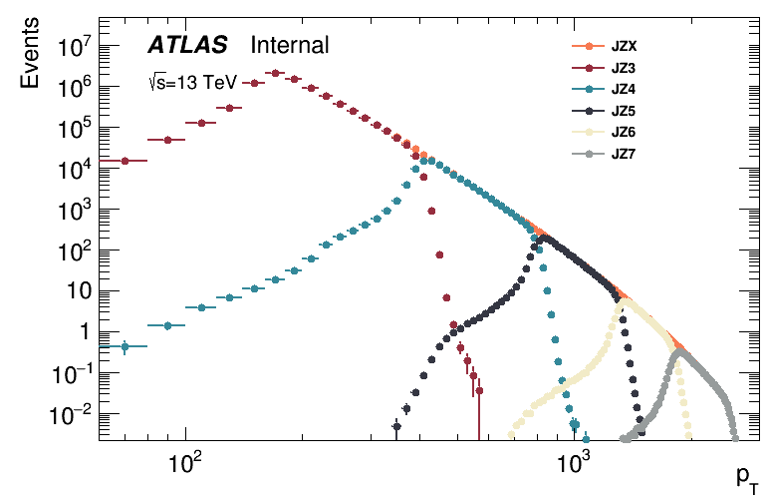
\includegraphics[width=0.4\textwidth]{figures/gbb/LeadJetCheck.png}
\caption{Distribution of $p_T$ of the leading anti-$k_t$ R=0.4 jet in each JZ slice and for all slices combined ``JZX''.}
  \label{fig:gbb-leadAkt4}
\end{figure}


\begin{table}[htpb]
\centering
\begin{tabular}{cccc}
Process & Name & ID & Generator \\
\hline 
\hline
Di-Jets & Pythia8\_EvtGen\_A14NNPDF23LO\_JZ3W & 361023 & Pythia  \\
Di-Jets & Pythia8\_EvtGen\_A14NNPDF23LO\_JZ4W & 361024 & Pythia  \\
Di-Jets & Pythia8\_EvtGen\_A14NNPDF23LO\_JZ5W & 361025 & Pythia  \\
Di-Jets & Pythia8\_EvtGen\_A14NNPDF23LO\_JZ6W & 361026 & Pythia  \\
Di-Jets & Pythia8\_EvtGen\_A14NNPDF23LO\_JZ7W & 361027 & Pythia  \\
\hline
\hline
\end{tabular}
\caption{Monte Carlo samples as used in the analysis. }
\label{tab:mc_samples1}
\end{table}


\subsection{Data}

The data samples used in this analysis were recorded by the ATLAS detector over the period June 2016 to December 2016, corresponding to data-taking periods A to L. This corresponds to an integrated luminosity of 33.1 fb${}^{-1}$ after application of basic data quality requirements via the standard ATLAS Good Run List\footnote{The official standard GRL for 2016 data (\url{data16_13TeV.periodAllYear_DetStatus-v83-pro20-15_DQDefects-00-02-04_PHYS_StandardGRL_All_Good_25ns.xml}) is used.}. The uncertainty on the integrated luminosity is 2.2\%. 



\clearpage

%-------------------------------------------------------------------------------
%\section{Simulated Samples}
%\label{sec:mc}
%-------------------------------------------------------------------------------
%
The simulated samples used in this analysis are provided by the MC15c
production campaign of the ATLAS MC Production
Group \cite{TWiki_AtlasProductionGroup}. 
Simulated samples are used for the SM Higgs boson
ggF and VBF production, and strong and electroweak \zjets{} production.

For all signal samples, the detector response is simulated with the \geantFour{}
package~\cite{Agostinelli:2002hh}.
For the \zjets{} background samples, the detector response is simulated 
with the fast-simulation
package \atlfastTwo{}~\cite{Richter-Was:683751}.
Pile-up effects are taken into account by using minimum bias events
generated with \pythia{}~\cite{Sjostrand:2014zea} where the mean number of interactions
per bunch crossing is adjusted to the data-taking period.

VBF and ggF Higgs boson samples are generated with the next-to-leading order (NLO)
generator \powheg{}~\cite{Nason:2004rx,Frixione:2007vw,Alioli:2010xd} using the
CT10 PDF set~\cite{Lai:2010vv} and interfaced with \pythia{} for parton showering
and fragmentation with the AZNLO tune.
%Alternative samples, obtained by processing the same generated events with 
%\herwig{}~\cite{Bahr:2008pv,Bellm:2015jjp}
%for parton showering and fragmentation, are used for assessing modeling uncertainties.
We use two \zjets{} samples generated with \madgraph{}~\cite{Alwall:2014hca} 
using the NNPDF PDF set~\cite{nnpdf} and interfaced with \pythia{} for parton showering
and fragmentation with the A14 tune. One sample is used to model QCD $Z$ production.
In this sample electro-weak (EWK) production of $Z$
(e.g., $q+q \rightarrow W^{+} + W^{-} + qq  \rightarrow Z + qq$)
is explicitly not generated. To improve the efficiency of the sample
for our final state, two light partons (light quarks or gluons) are
required in the final state ($pp \rightarrow Z+ q/g + q/g$).
The second sample contains exclusively electroweak $Z$ production.
The cross sections of MC samples we use in this analysis are presented Table. \ref{tab:xsec}.

\begin{table}[htpb]
\centering
\caption{MC sample cross section times branching ratio}
\label{tab:xsec}
\begin{tabular}{|l|l|l|l|l|}
\hline
                   & VBF $h\rightarrow b \bar b$  & ggF $h\rightarrow b \bar b$  & QCD \zjets{} & EWK \zjets{} \\ \hline
$\sigma \times$ Br (Pb) & 2.22 & 25.91 & 666.52         & 4.86         \\ \hline
\end{tabular}
\end{table}


\clearpage

%-------------------------------------------------------------------------------
\section{Object Definitions}
\label{sec:objects}
%-------------------------------------------------------------------------------
\label{sec:gbb-obj}

\subsubsection{Primary Vertex and Track Selection}
The primary hard scattering vertex for the event is chosen as the vertex with the highest $\sum p_{T}^{2}$ where the sum runs over the tracks associated to the vertex. Tracks which are used to determine the primary vertex need to pass the following selection:
\begin{enumerate}
    \item $p_T>$ 0.5 GeV
    \item Number of Pixel hits greater than 1
    \item Number of SCT hits greater than 6
    \item $|d_0|<1$mm, with respect to primary vertex
    \item $|z_0\sin(\theta)|<1$mm, with respect to primary vertex
\end{enumerate}

\subsubsection{Jet Selection}
In this study we use $R$=1.0 calorimeter jets and $R=0.2$ track jets. Calorimeter jets are clustered in $y-\phi$ space using the anti-$k_t$~\cite{Cacciari:2008gp} algorithm with $R=1.0$ reconstructed from topological calorimeter clusters~\cite{TopoClusters} using the local cluster weighting (LCW) algorithm \cite{EndcapTBelectronPion2002} and calibrated to account for the detector response. Track jets are reconstructed clustering inner detector tracks using the anti-$k_t$ algorithm and are required to have at least two tracks.

\noindent The $R = 1.0$ calorimeter jets are groomed using the trimming procedure~\cite{Krohn:2009th}, whereupon the $k_{t}$ subjets ~\cite{Cacciari200657} with $R=0.3$ are discarded if the fractional $p_{T}$ of the subject relative to the whole $R=1.0$ jet satisfies $f_\text{ cut}<0.05$.  

\noindent The $R=0.2$ track jets are subject to the following selection, 
\begin{enumerate}
	\item $p_T>$10 GeV
	\item $|\eta|<2.5$	
	\item The track jet originates from the primary vertex (OriginIndex==0)
\end{enumerate}

\subsubsection{$b$-tagging}

Jets are identified as $b$-jets using the multivariate discriminant $MV2c10$ \cite{btag} which includes impact parameter and secondary vertex information as inputs.  The chosen $MV2c10$ working point corresponds to an average $b$-tagging efficiency of 70\% for $b$-jets in simulated $t\bar{t}$ events.  

\subsubsection{Ghost Association of Jets}

We adopt a robust matching algorithm called ghost association~\cite{area} to associate $R=0.2$ track jets to $R=1.0$ jets. With this method, the 4-vector of the physics object is added to the inputs of the jet clustering algorithm but the object 4-vector has the $p_T$ set to an infinitesimal amount, hence called a ghost.  Jet clustering is then performed. This way, the ghost does not alter the clustering history, but the 4-vectors retain the original object direction and are clustered into a jet if the ghost 4-vector points within the active area of the jet.

\subsubsection{Flavor Labeling of Jets in Simulation}

The flavor content of the track jet is determined by ghost matching truth particles (weakly decaying $B$-hadrons and $c$-hadrons) to the track jet. For each jet, if a $B$-hadron is found to be associated to the jet, then the jet is labeled as a $b$-jet.  If there are no $B$-hadrons but a $c$-hadron is found to be associated to the jet, then the jet is labeled as a $c$-jet. Otherwise, the jet is labeled as a light-flavored jet. 

\subsubsection{Truth Jets}

All final state truth particles (ignoring truth pileup) with mean lifetimes longer than 30 ps, except muons and neutrinos, are used as input to the clustering of truth jets. 


\clearpage

%-------------------------------------------------------------------------------
\section{Event Selection}
\label{sec:evtselection}
%-------------------------------------------------------------------------------

\label{sec:gbb-eventselection}

The overall event selection strategy aims to enhance the purity of gluon splitting to $b \bar b$ events. The gluon splitting process dominates at low $\Delta R$. To isolate this process, we require events to have one $R=1.0$ jet, which is the proxy of the gluon. The $R=1.0$ jet is required to have at least two ghost associated $R=0.2$ track jets, which are proxies of the splitting products of the gluon. The leading track jet is then $b$-tagged. 

The un-prescaled HLT item \textbf{HLT\_j420\_a10\_lcw\_L1J100} triggers on events which have $R=1.0$ jets. The leading $R=1.0$ jet is required to have $p_T>450$ GeV to be on the trigger efficiency pleateu. 

The detailed event selection goes as the following:
\begin{enumerate}
	\item MC events are subject to event cleaning: the average $p_T$ of leading two $R=0.4$ reco jets is less than 1.4 times the $p_T$ of the leading $R=0.4$ truth jet. 
	\item Pass the $R=1.0$ single jet trigger: \textbf{HLT\_j420\_a10\_lcw\_L1J100}
	\item The leading $R=1.0$ jet in the event has $p_T>450$ GeV
        \item The leading $R=1.0$ jet in the event has at least two $R=0.2$ jets ghost matched
	\item The leading track jet passes the 60\% $b$-tagging efficiency working point
\end{enumerate}


\subsubsection{Kinematic Reweighting}

After the event selection is made, we observed that there are mild disagreements between data and MC of jet kinematic properties. The impact of the disagreement on the final results is explored by reweighting the MC, event-by-event, by the ratio of the two dimensional leading and sub-leading track jets $p_T$ distributions between MC and data\footnote {Note that $b$-tagging scale factors are applied prior to re-weighting.}. The mis-modeling could arise from the overall di-jet cross section, $R=1.0$ ghost matching efficiency and $b$-tagging efficiency as a function of $p_T$ in the particular event topology.

The re-weighting factors are shown in Fig.~\ref{fig:gbb-reweightmap}. The data and MC comparison for the $p_{T}$ and $\eta$ of the $R=1.0$ and track jets are shown before applying $b$-tagging and after applying $b$-tagging and kinematics reweighting in Fig.~\ref{fig:gbb-pT_largeR},\ref{fig:gbb-eta_largeR},\ref{fig:gbb-pT_leadtrkjets},\ref{fig:gbb-pT_subtrkjets},\ref{fig:gbb-eta_leadtrkjets},\ref{fig:gbb-eta_subtrkjets}.

The impact of the re-weighting is assessed in Sec.\ref{sec:gbb-data_mc_comp}. We do not find the reweighting affects the flavor fit in any significant way and hence do not apply the reweighting for the nominal results.

\begin{figure}[htbp]
  \centering
 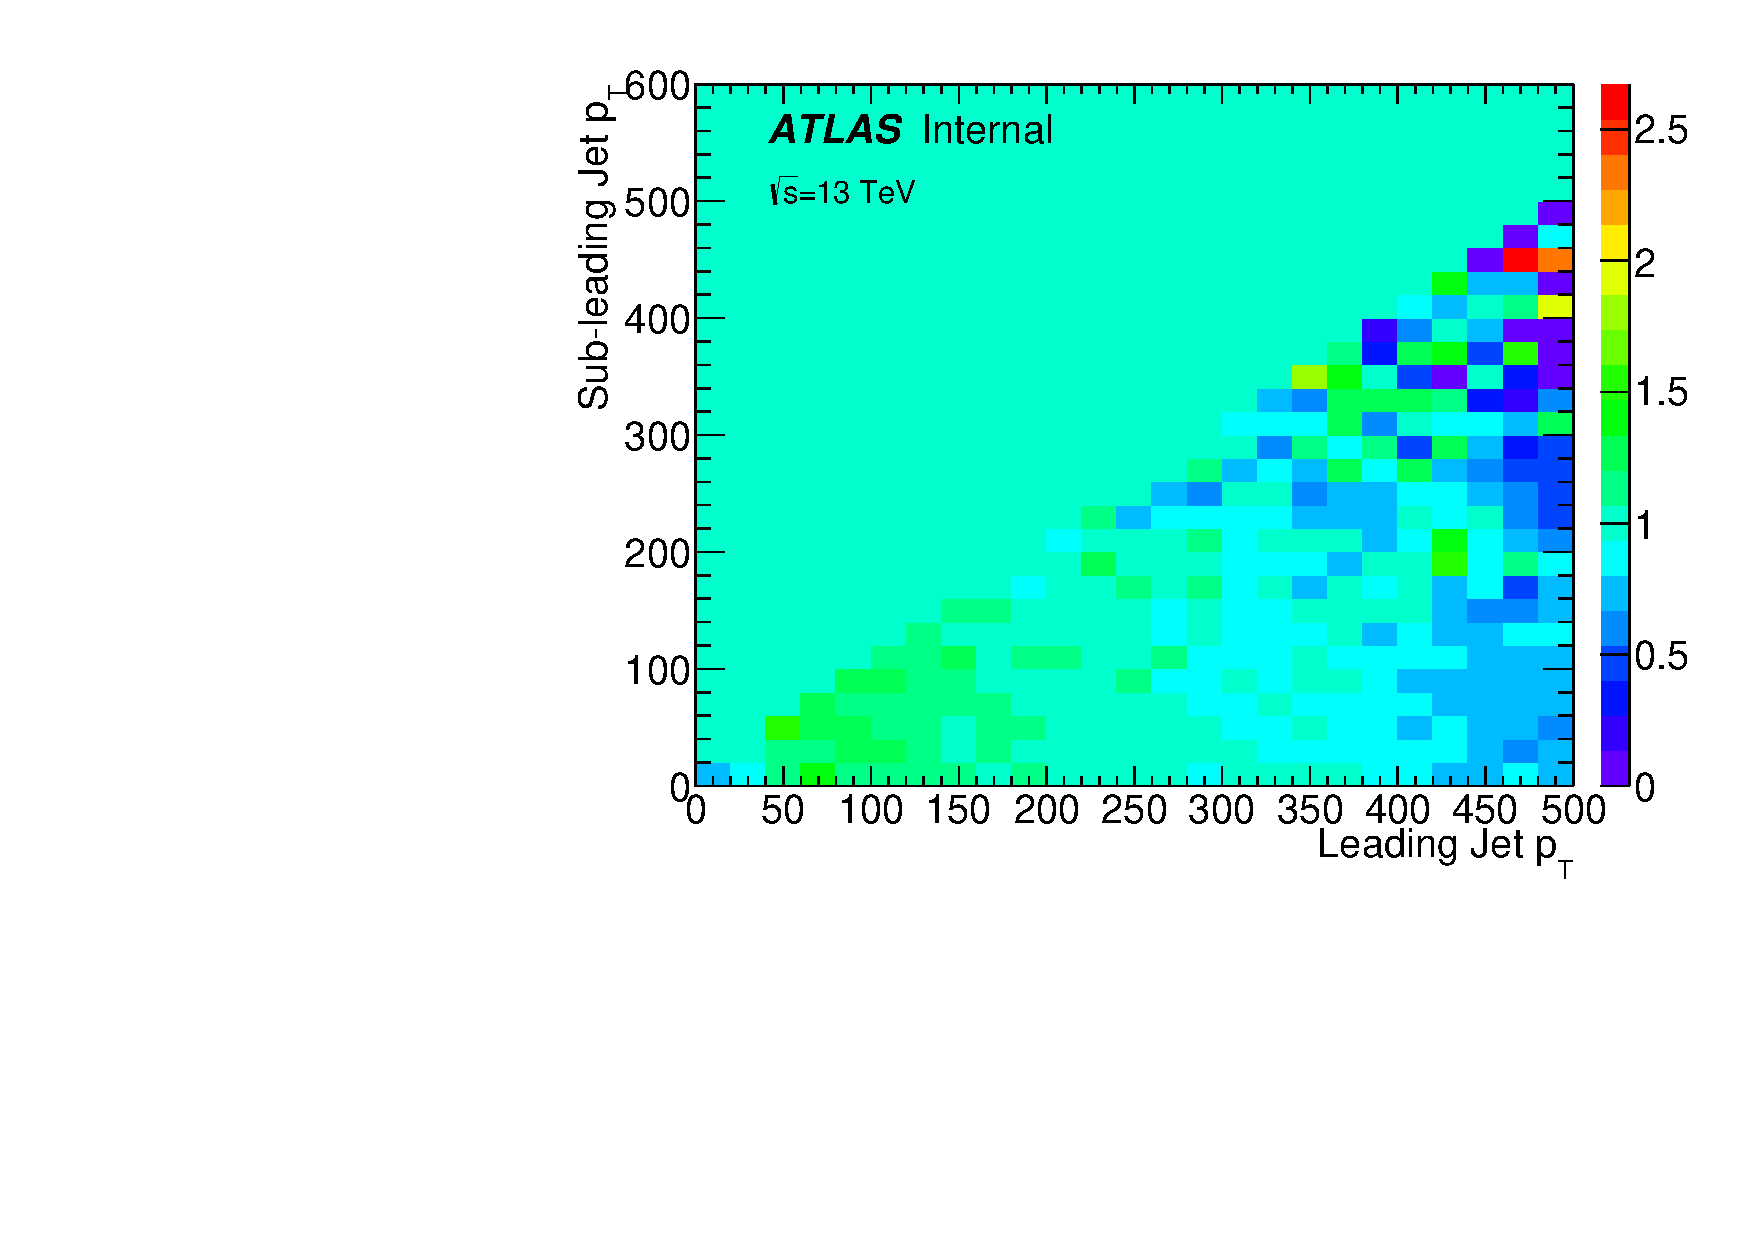
\includegraphics[width=0.6\textwidth]{figures/gbb/pTReweightMap.pdf}
\caption{The re-weighting factor applied to MC as a function of leading and sub-leading track jet $p_T$.}
  \label{fig:gbb-reweightmap}
\end{figure}


\begin{figure}[htbp]
  \centering
 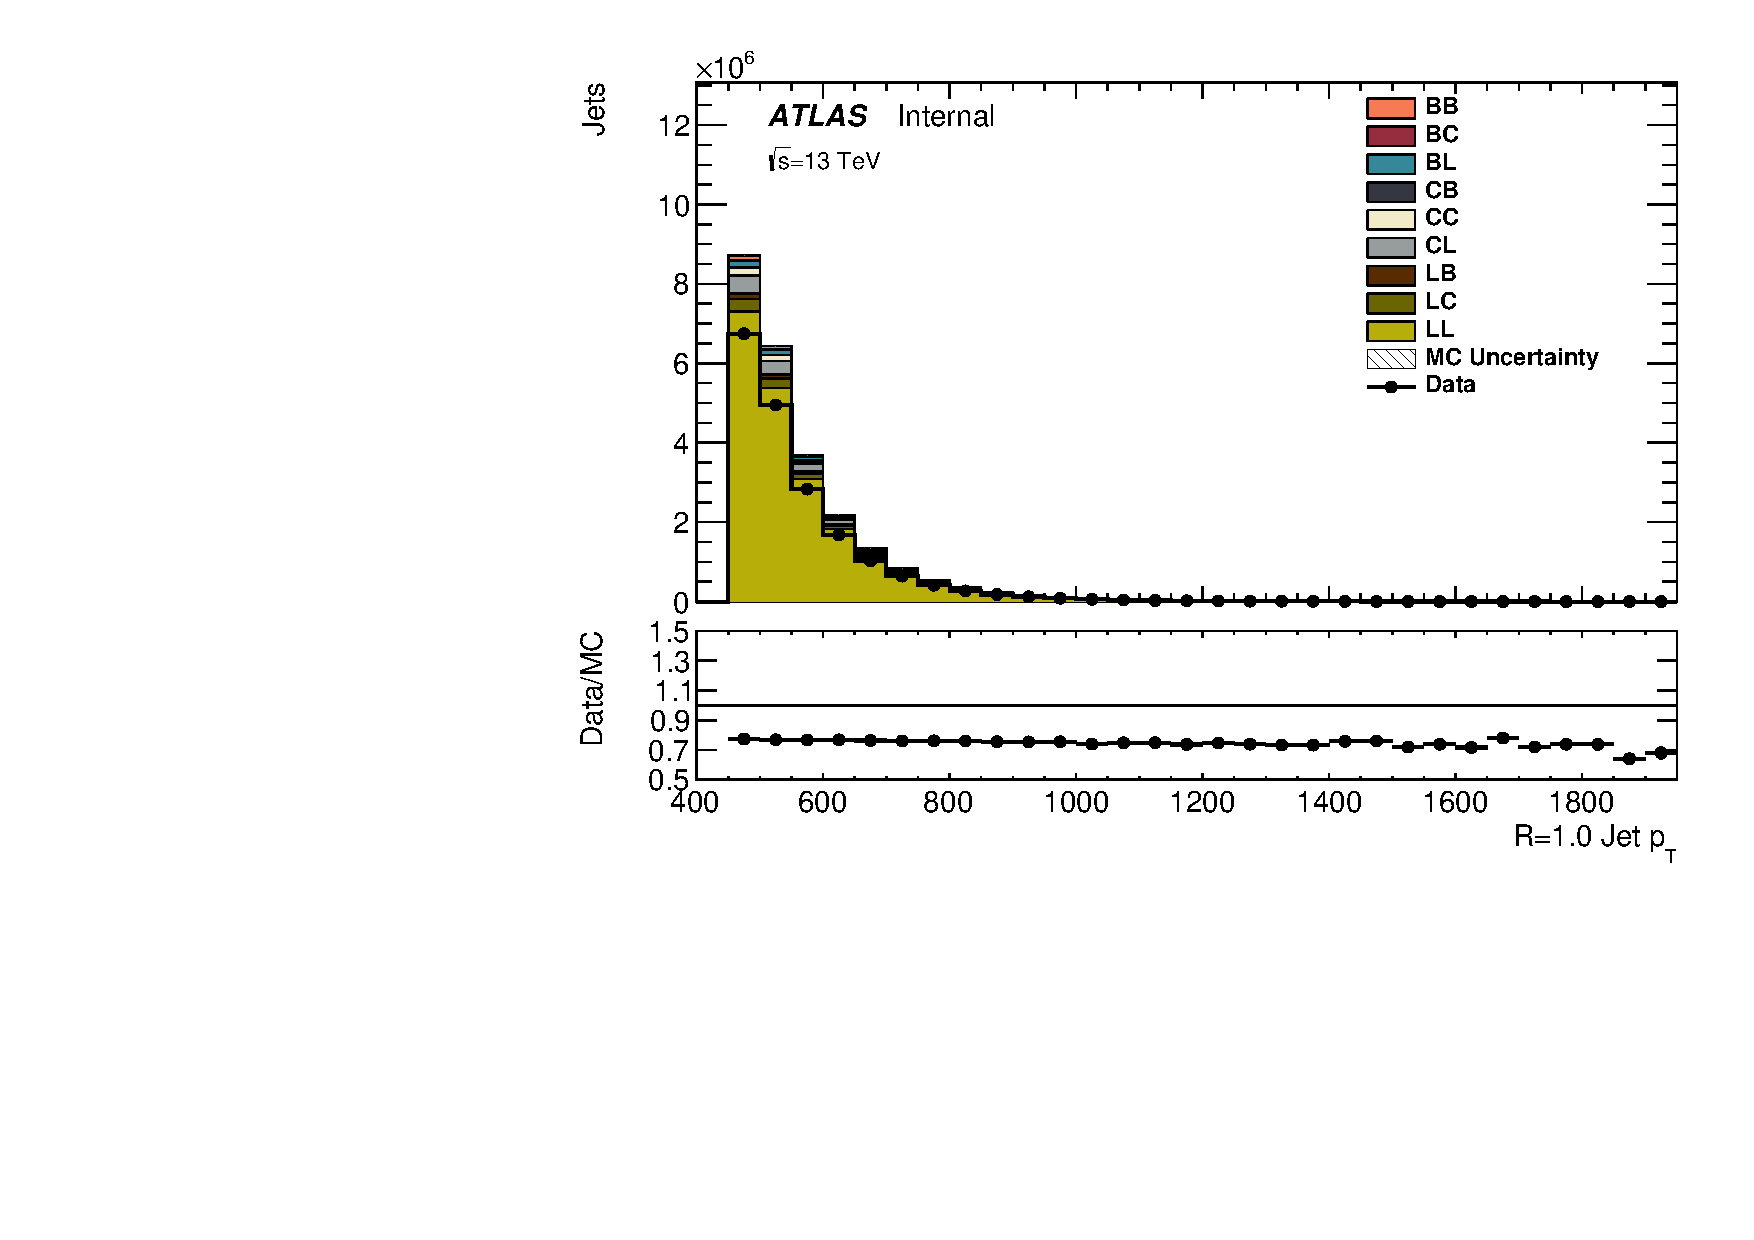
\includegraphics[width=0.45\textwidth]{figures/gbb/LargeRJet_pT_NoReweight.pdf}
 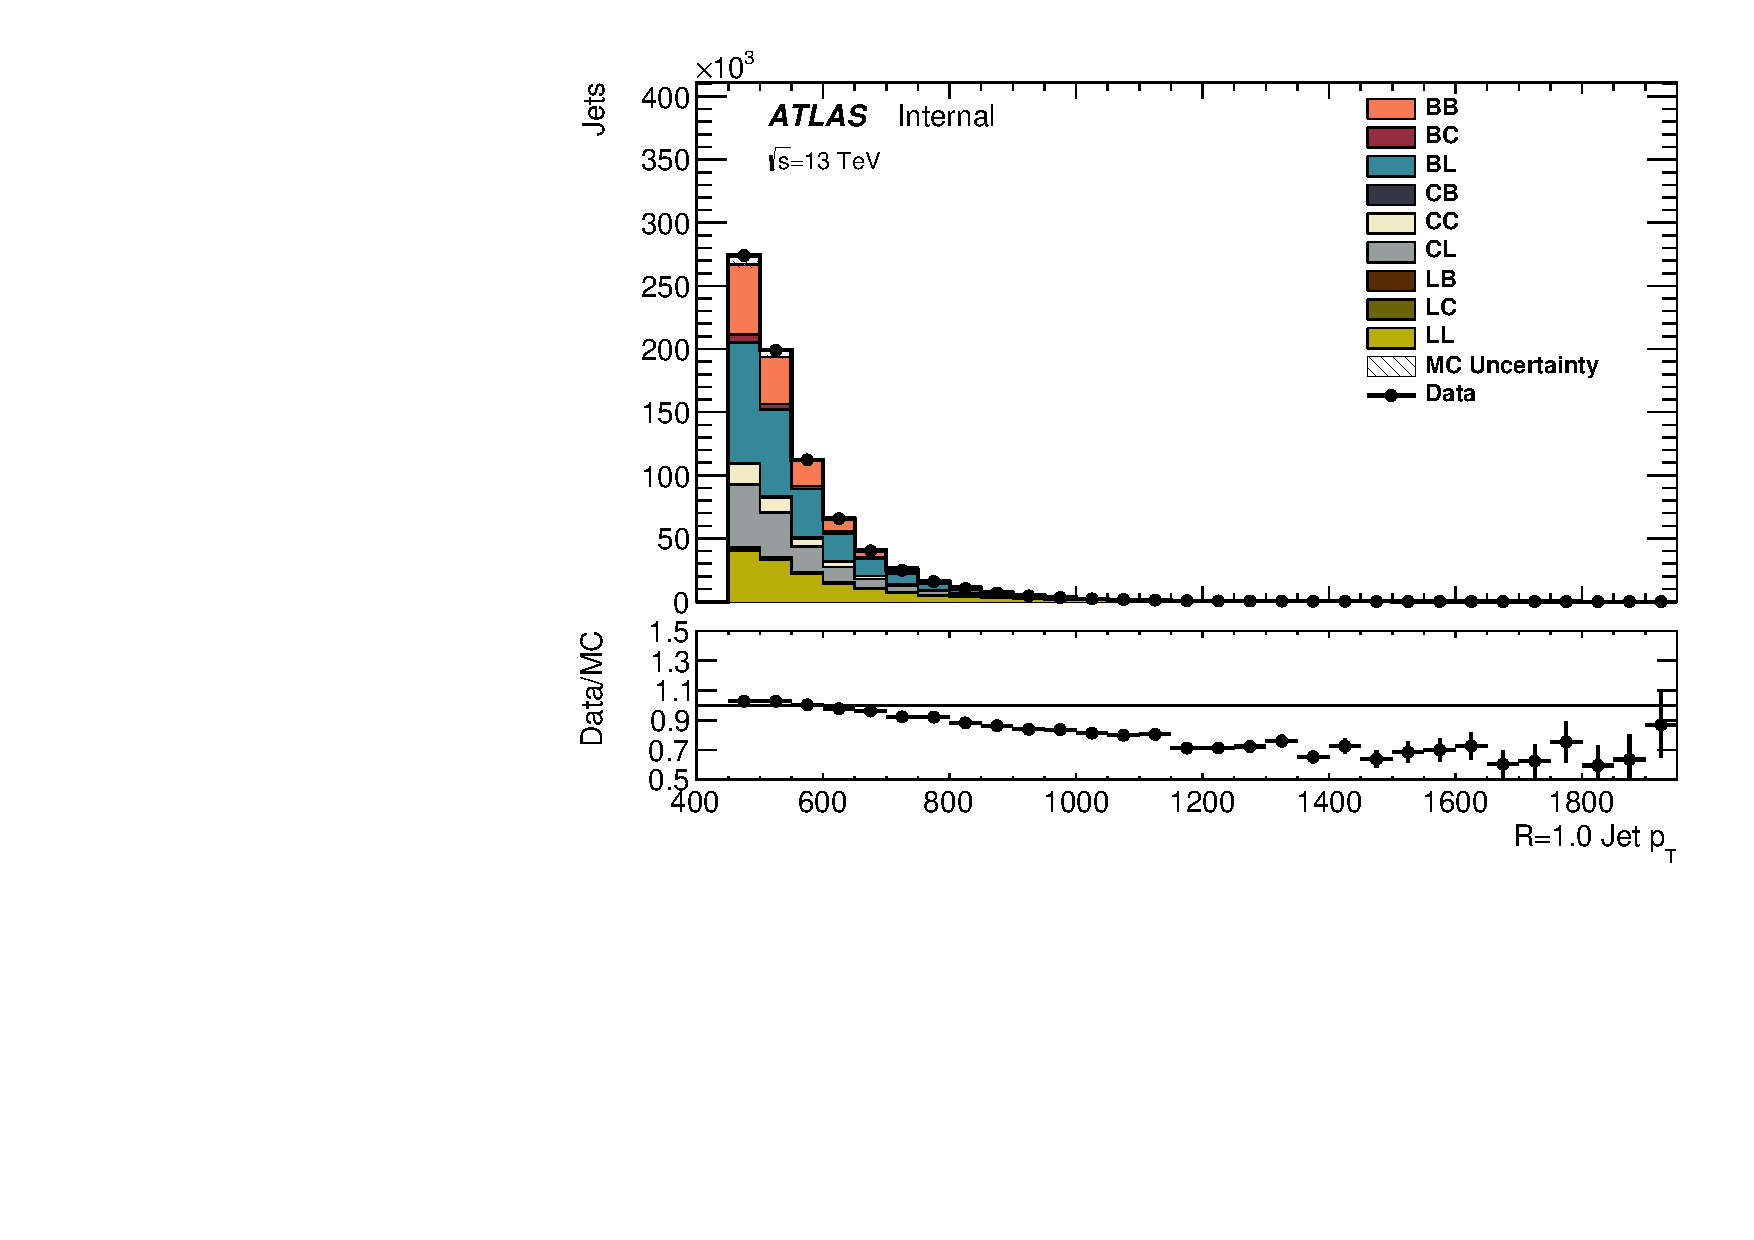
\includegraphics[width=0.45\textwidth]{figures/gbb/LargeRJet_pT_PreReweight.pdf}\\ 
 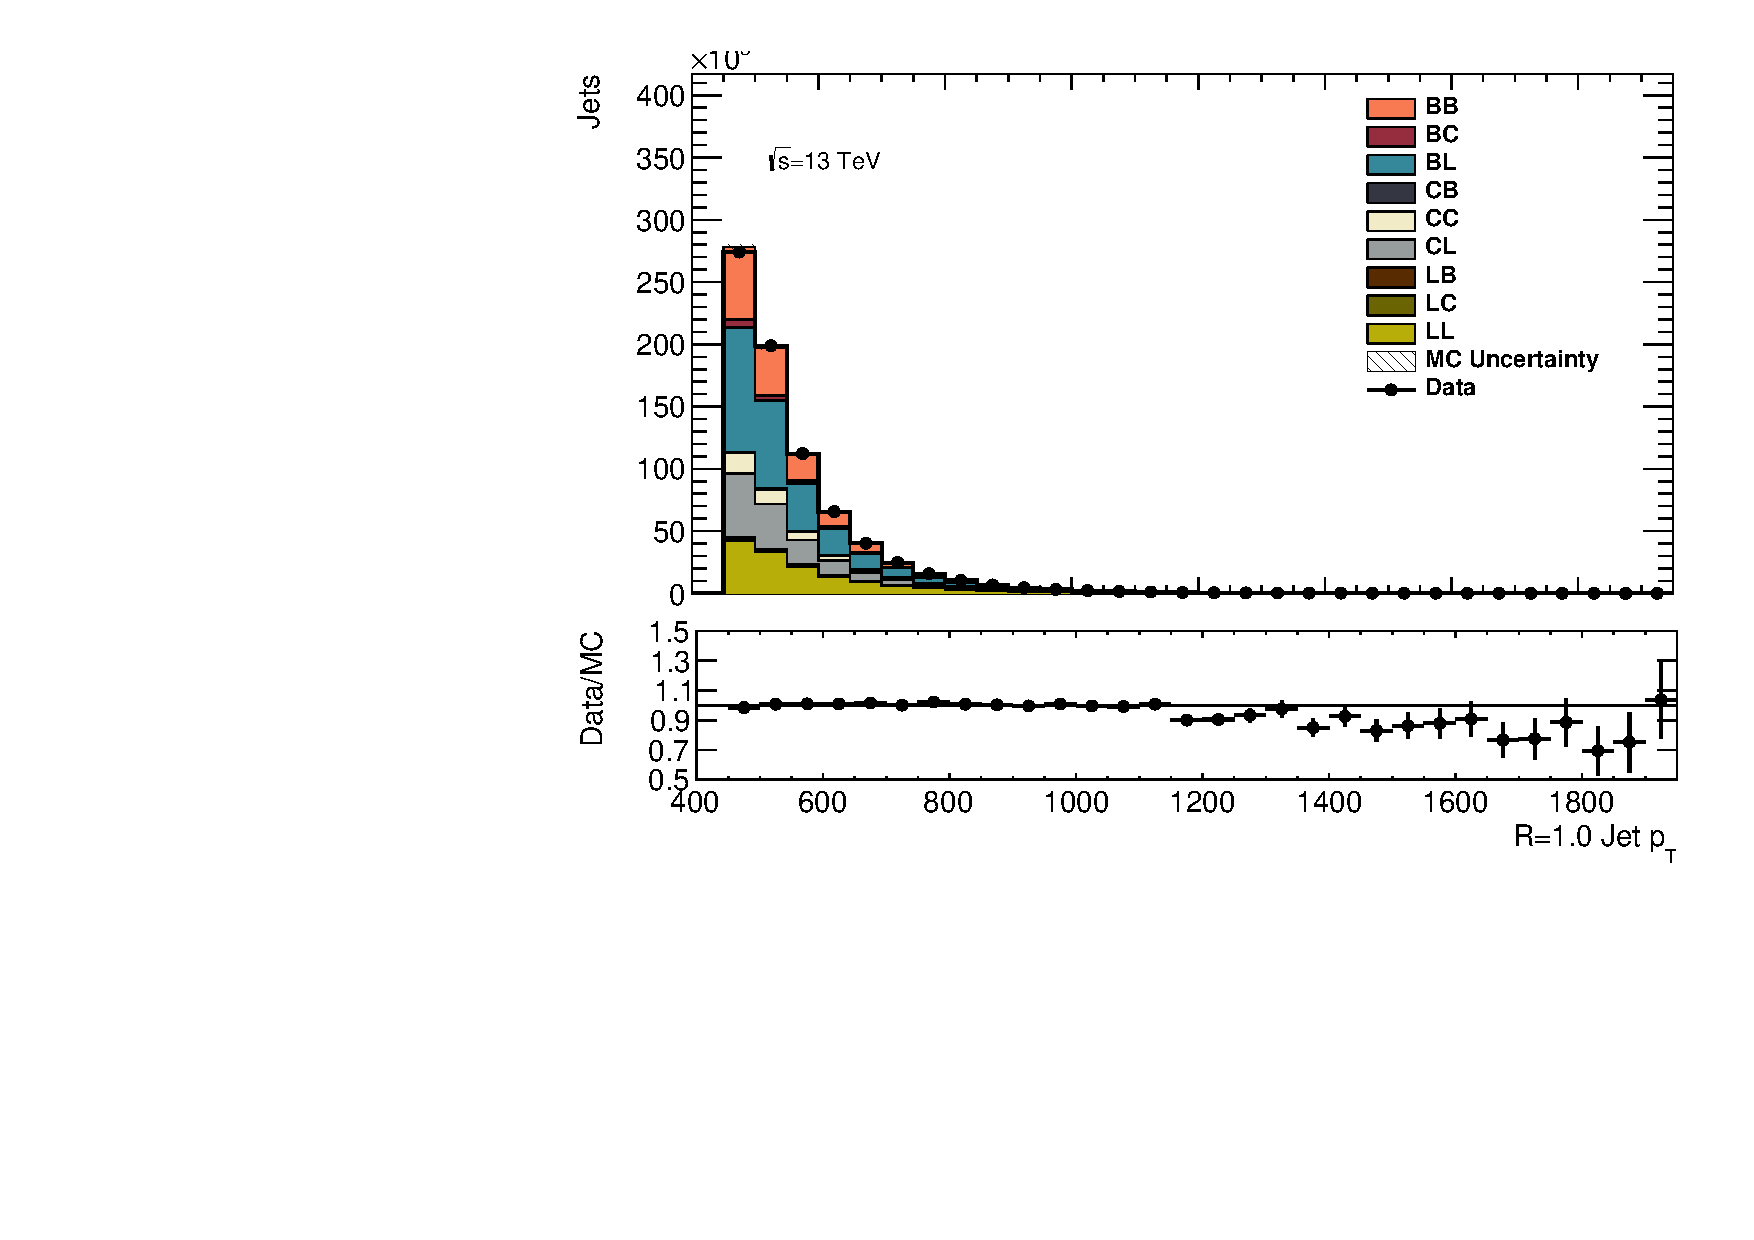
\includegraphics[width=0.45\textwidth]{figures/gbb/LargeRJet_pT_Reweight.pdf}
\caption{Data/MC comparison of $R=1.0$ jet $p_T$ before applying $b$-tagging (top left), post $b$-tagging without kinematic reweighting (top right) and post $b$-tagging with kinematic reweighting (bottom). The label of the $R=1.0$ jet flavor content ``XY'' denotes the leading and sub-leading track jet flavor. For example, the flavors of the leading and sub-leading track jet of a ``BL'' $R=1.0$ jet are `B' and `Light' respectively.}
  \label{fig:gbb-pT_largeR}
\end{figure}


\begin{figure}[htbp]
  \centering
 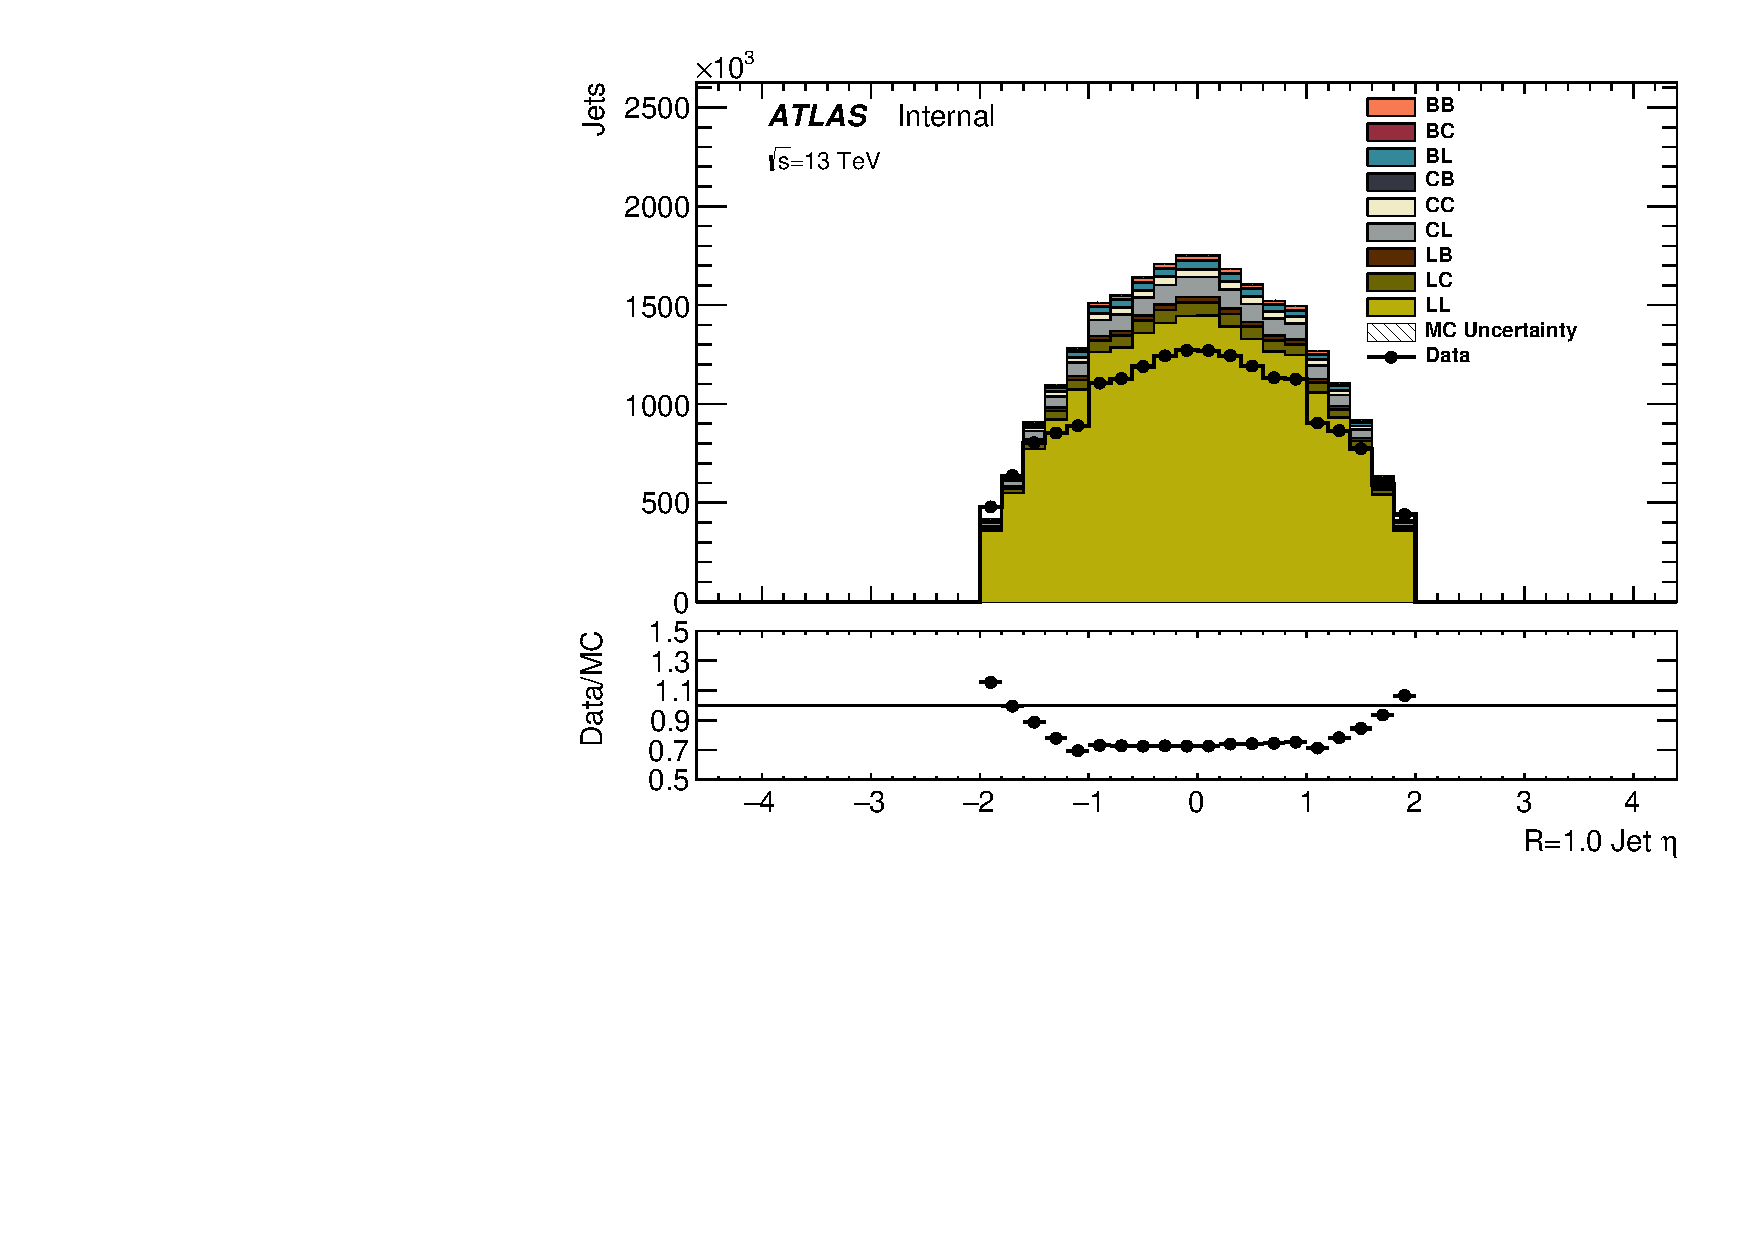
\includegraphics[width=0.45\textwidth]{figures/gbb/LargeRJet_eta_NoReweight.pdf}
 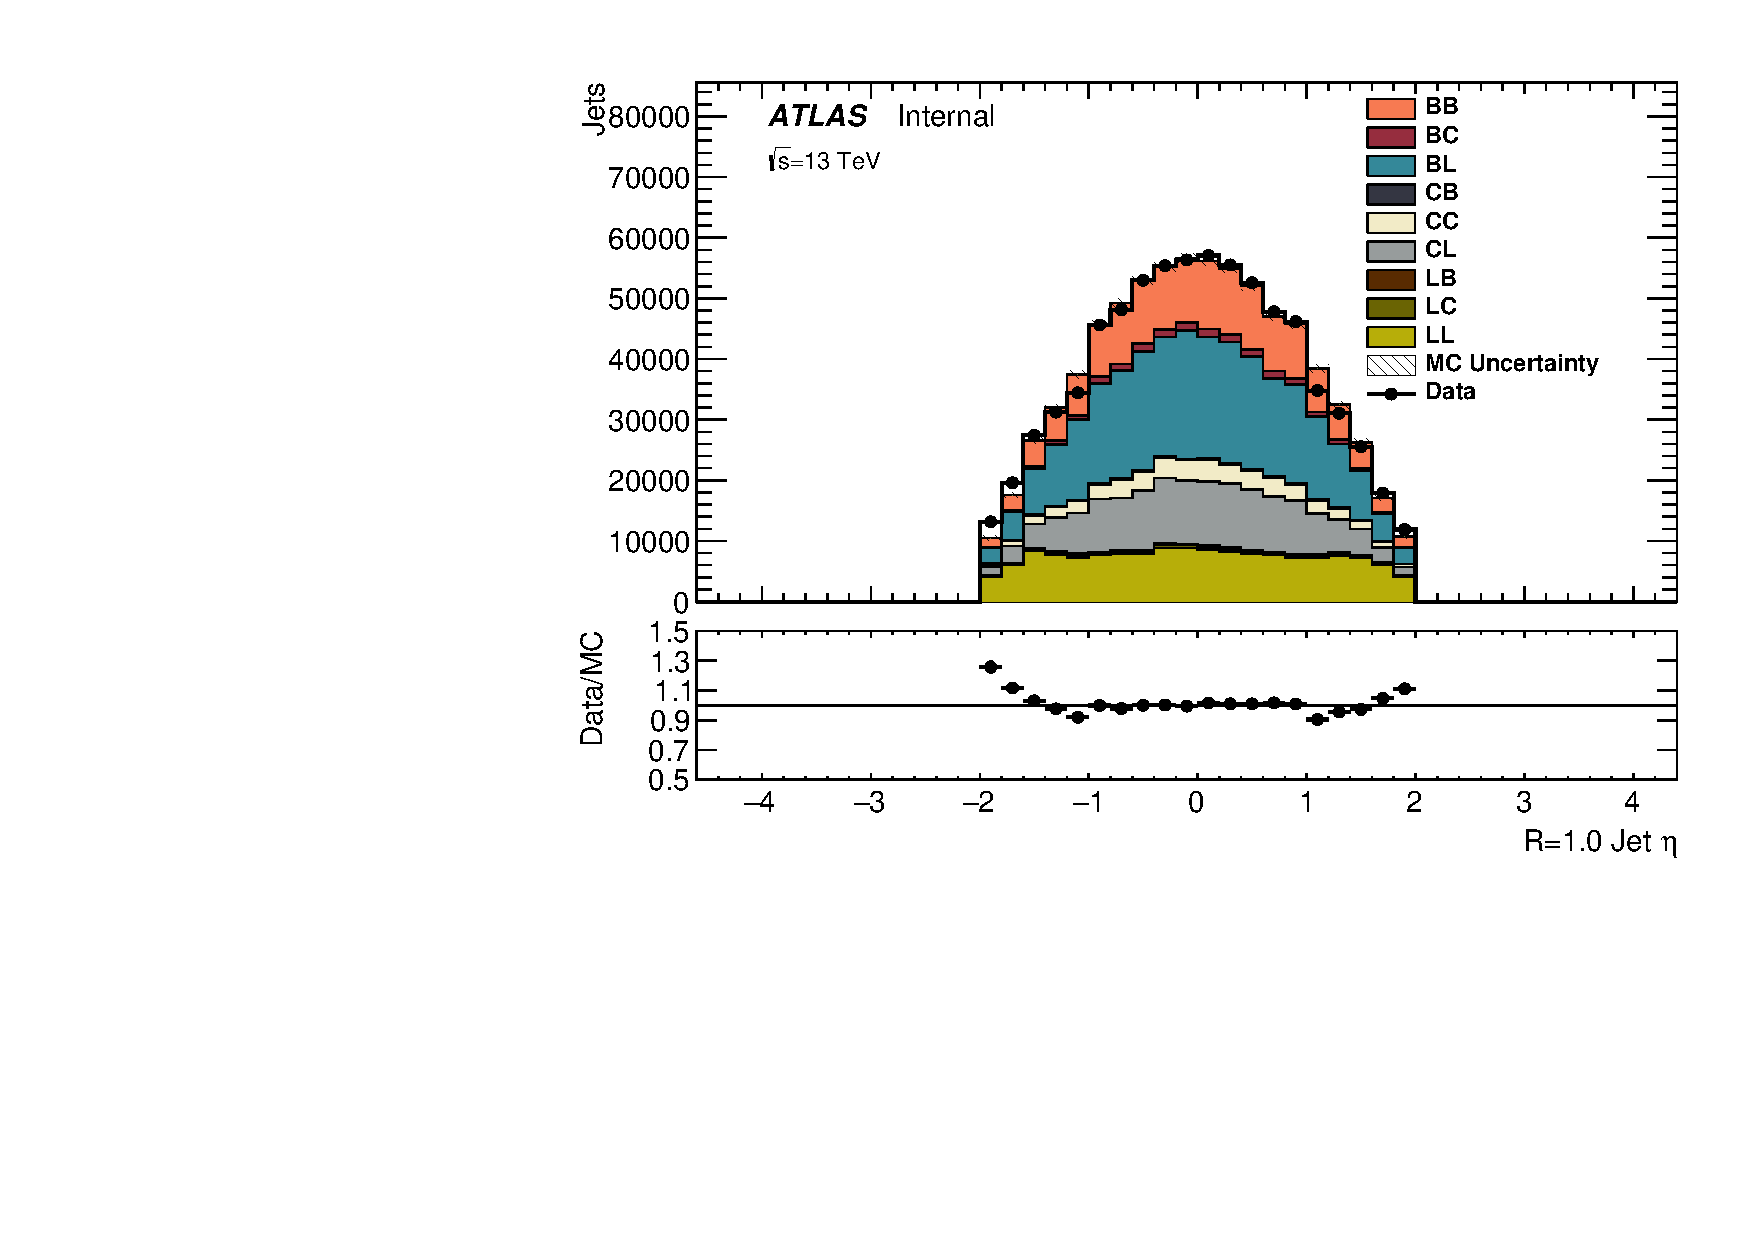
\includegraphics[width=0.45\textwidth]{figures/gbb/LargeRJet_eta_PreReweight.pdf}\\
 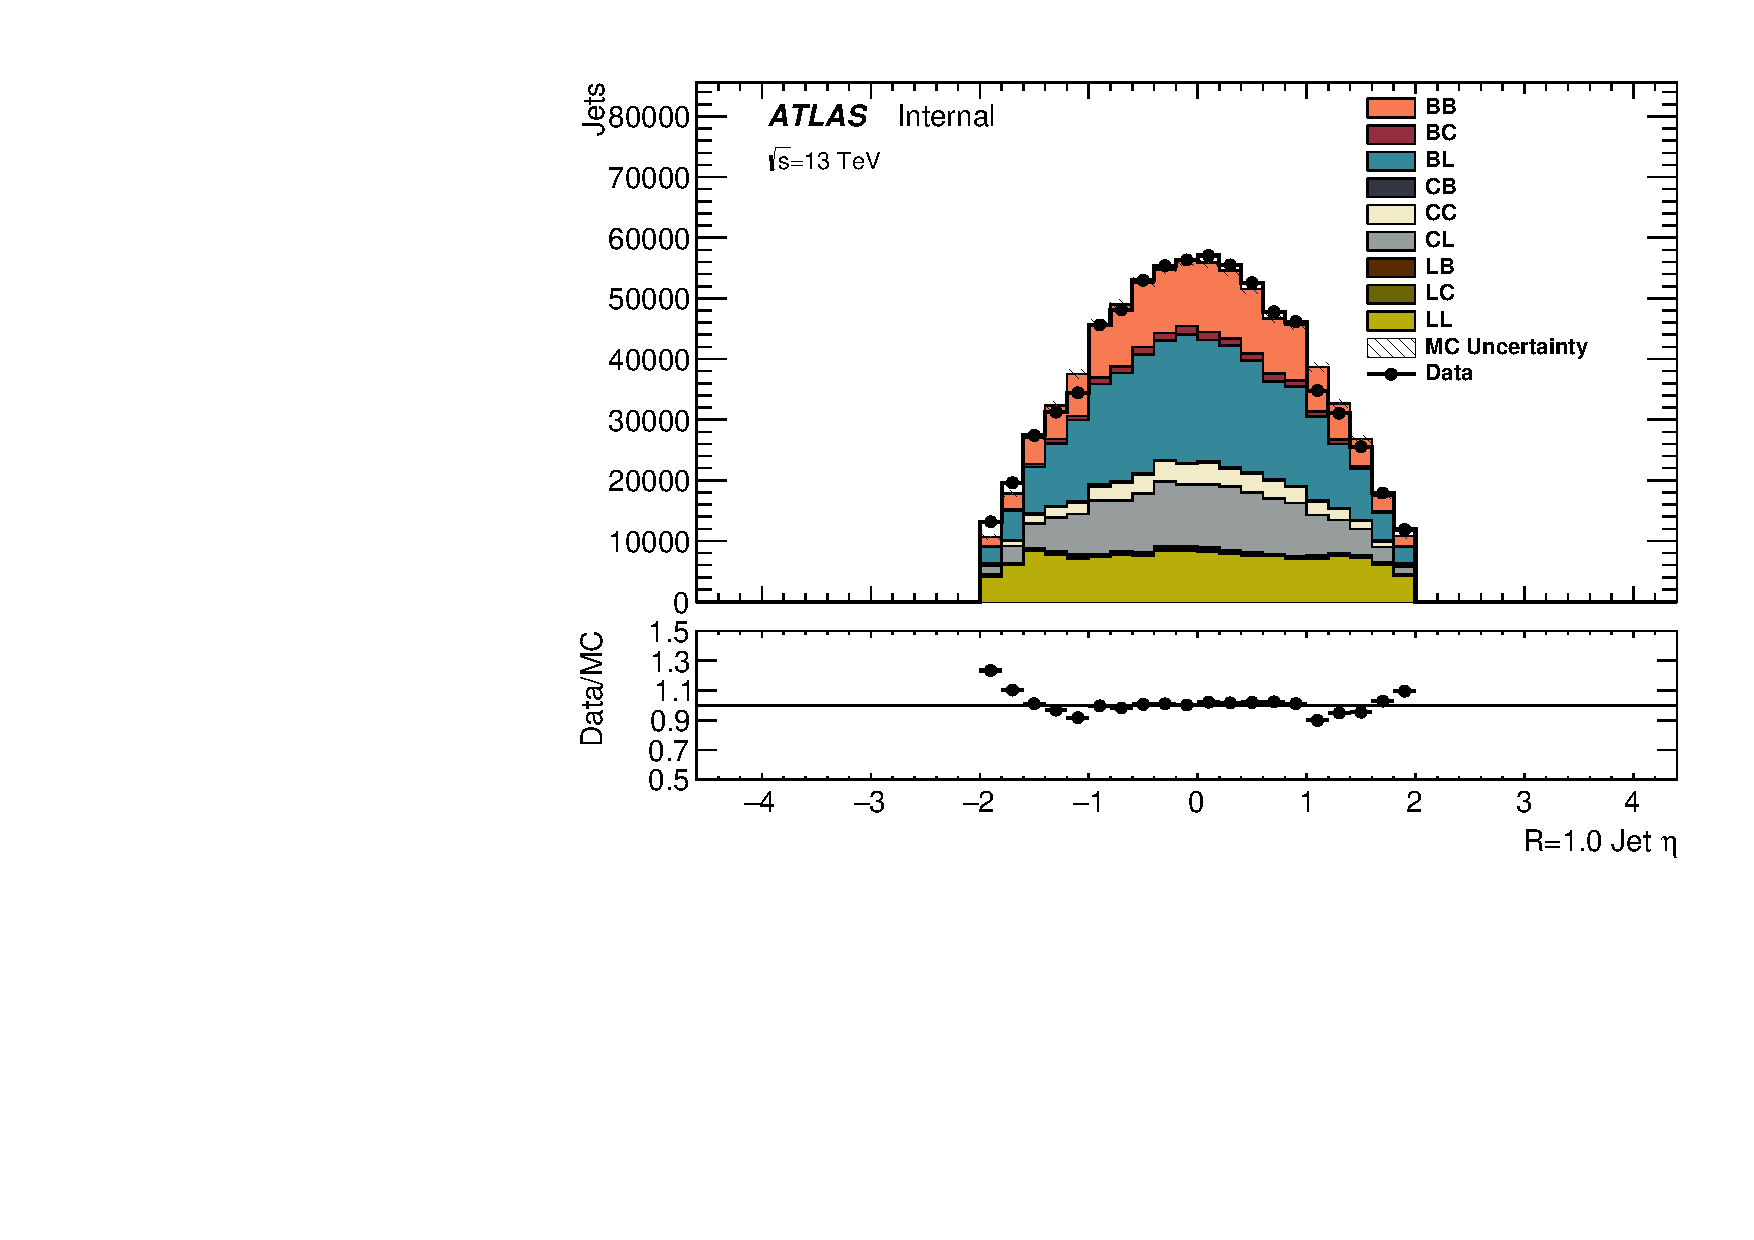
\includegraphics[width=0.45\textwidth]{figures/gbb/LargeRJet_eta_Reweight.pdf}
\caption{Data/MC comparison of $R=1.0$ jet $\eta$ before applying $b$-tagging (top left), post $b$-tagging without kinematic reweighting (top right) and post $b$-tagging with kinematic reweighting (bottom). The label of the $R=1.0$ jet flavor content ``XY'' denotes the leading and sub-leading track jet flavor. For example, the flavors of the leading and sub-leading track jet of a ``BL'' $R=1.0$ jet are `B' and `Light' respectively.}
  \label{fig:gbb-eta_largeR}
\end{figure}



\begin{figure}[htbp]
  \centering
 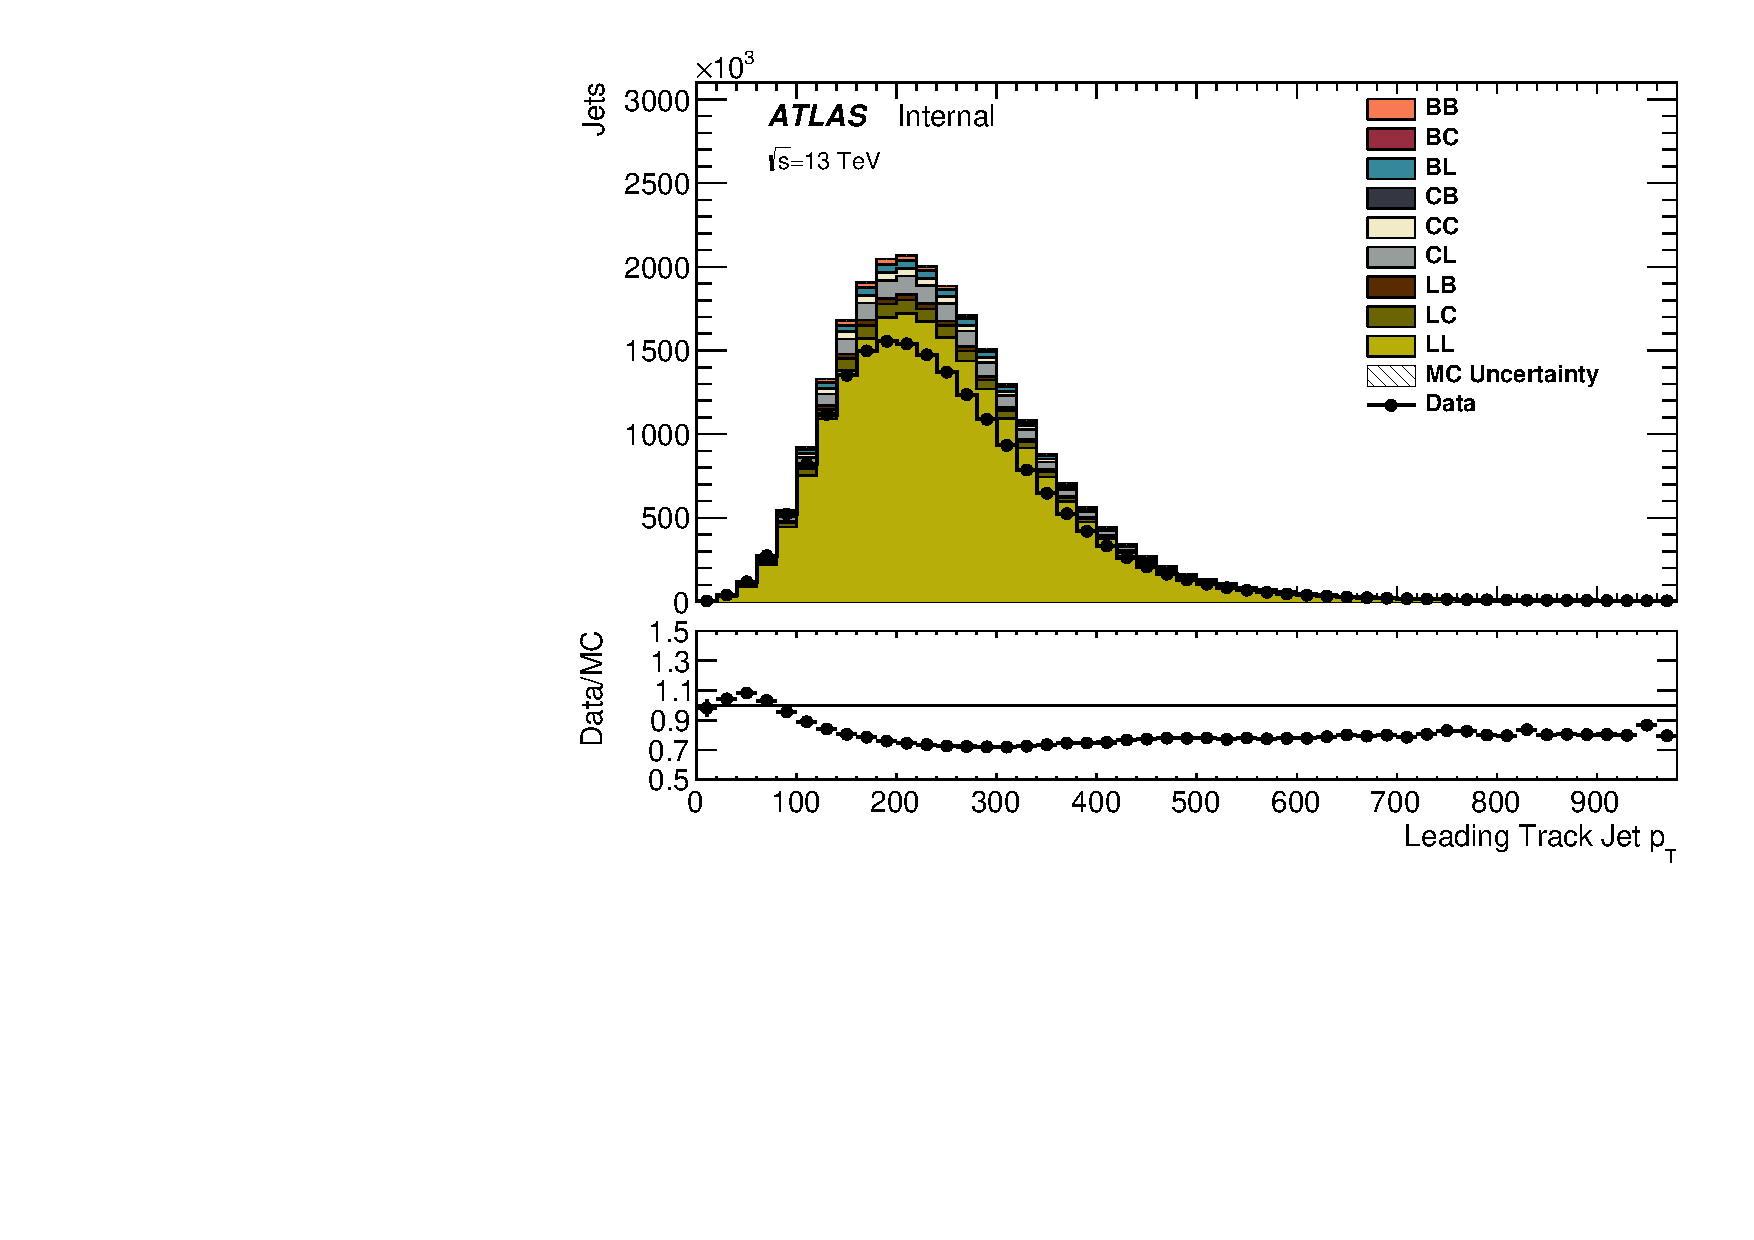
\includegraphics[width=0.45\textwidth]{figures/gbb/LeadTrkJet_pT_NoReweight.pdf}
 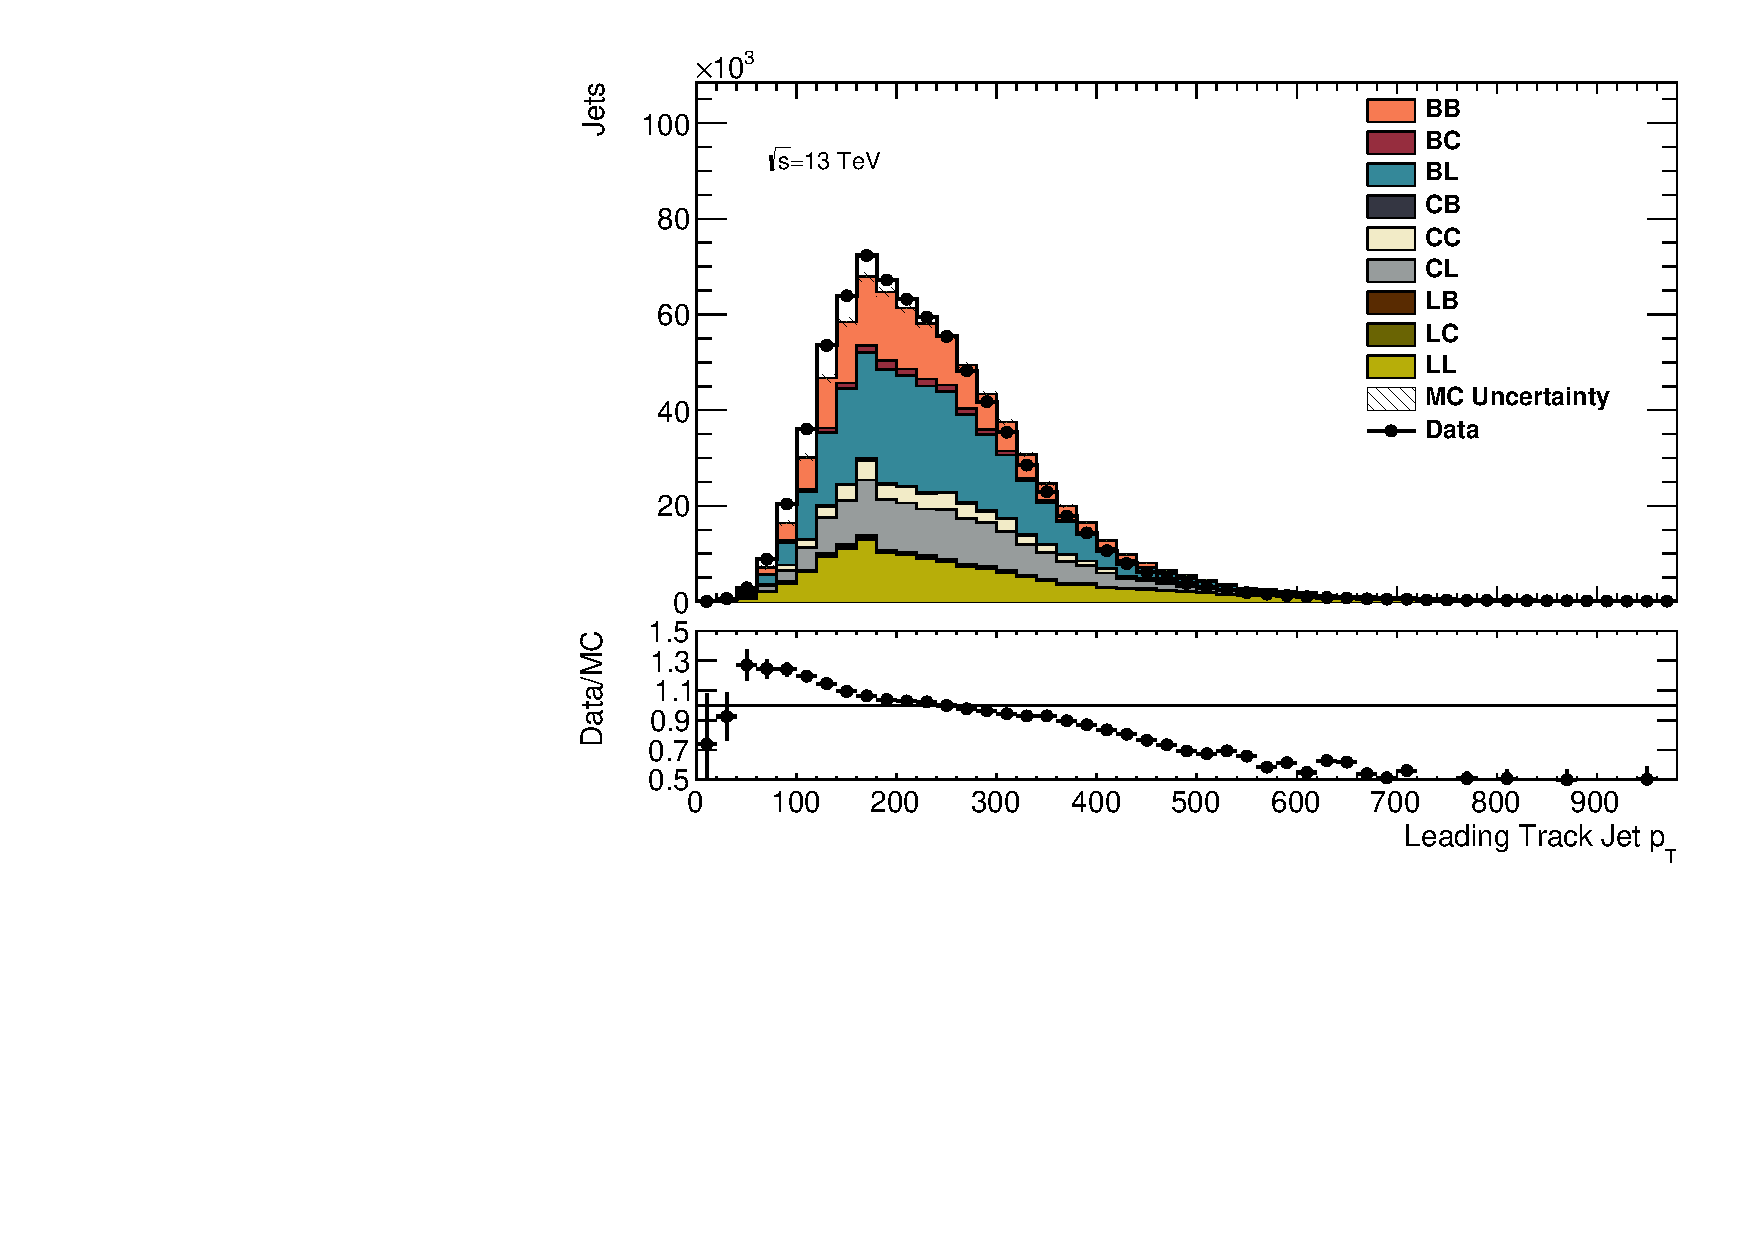
\includegraphics[width=0.45\textwidth]{figures/gbb/LeadTrkJet_pT_PreReweight.pdf}\\
 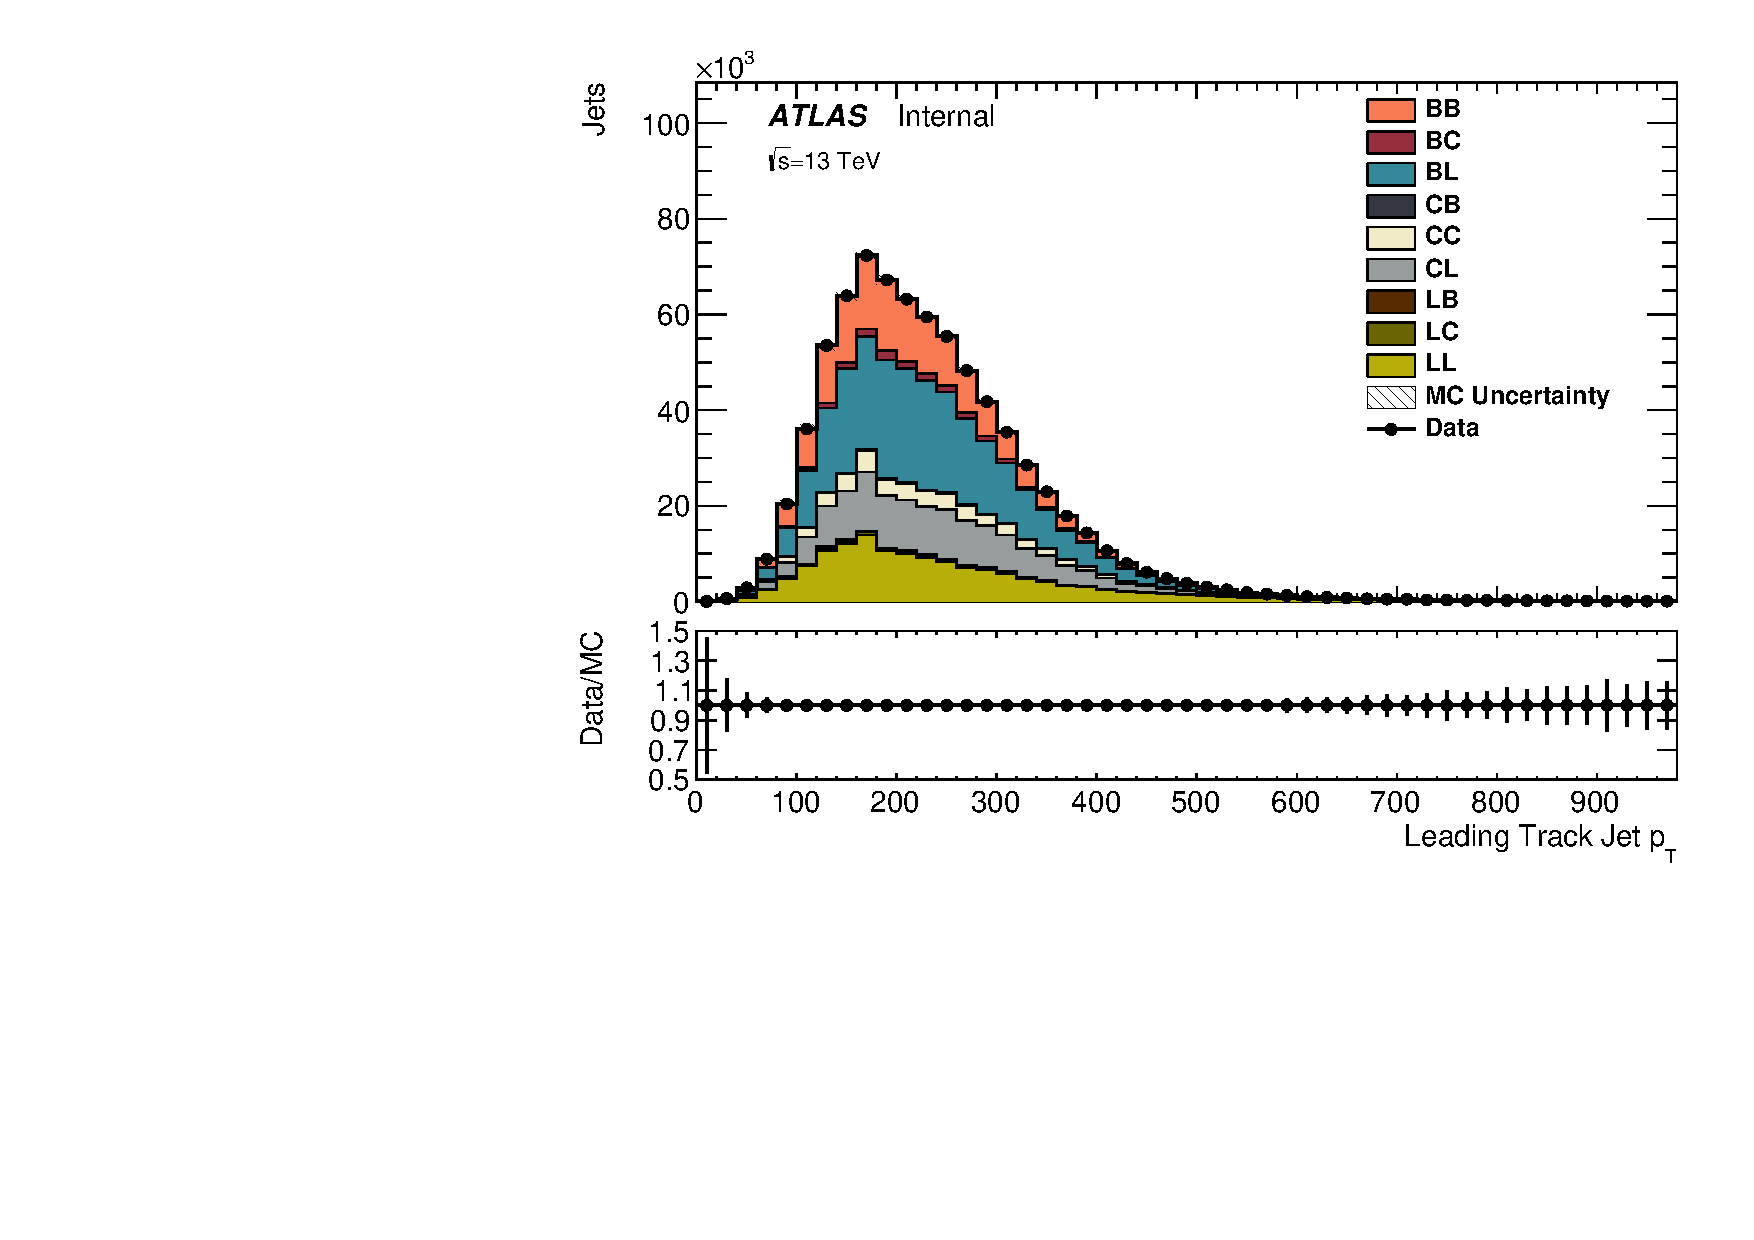
\includegraphics[width=0.45\textwidth]{figures/gbb/LeadTrkJet_pT_Reweight.pdf}
\caption{Data/MC comparison of leading track jets $p_T$ before applying $b$-tagging (top left), post $b$-tagging without kinematic reweighting (top right) and post $b$-tagging with kinematic reweighting (bottom). The label of the $R=1.0$ jet flavor content ``XY'' denotes the leading and sub-leading track jet flavor. For example, the flavors of the leading and sub-leading track jet of a ``BL'' $R=1.0$ jet are `B' and `Light' respectively.}
  \label{fig:gbb-pT_leadtrkjets}
\end{figure}


\begin{figure}[htbp]
  \centering
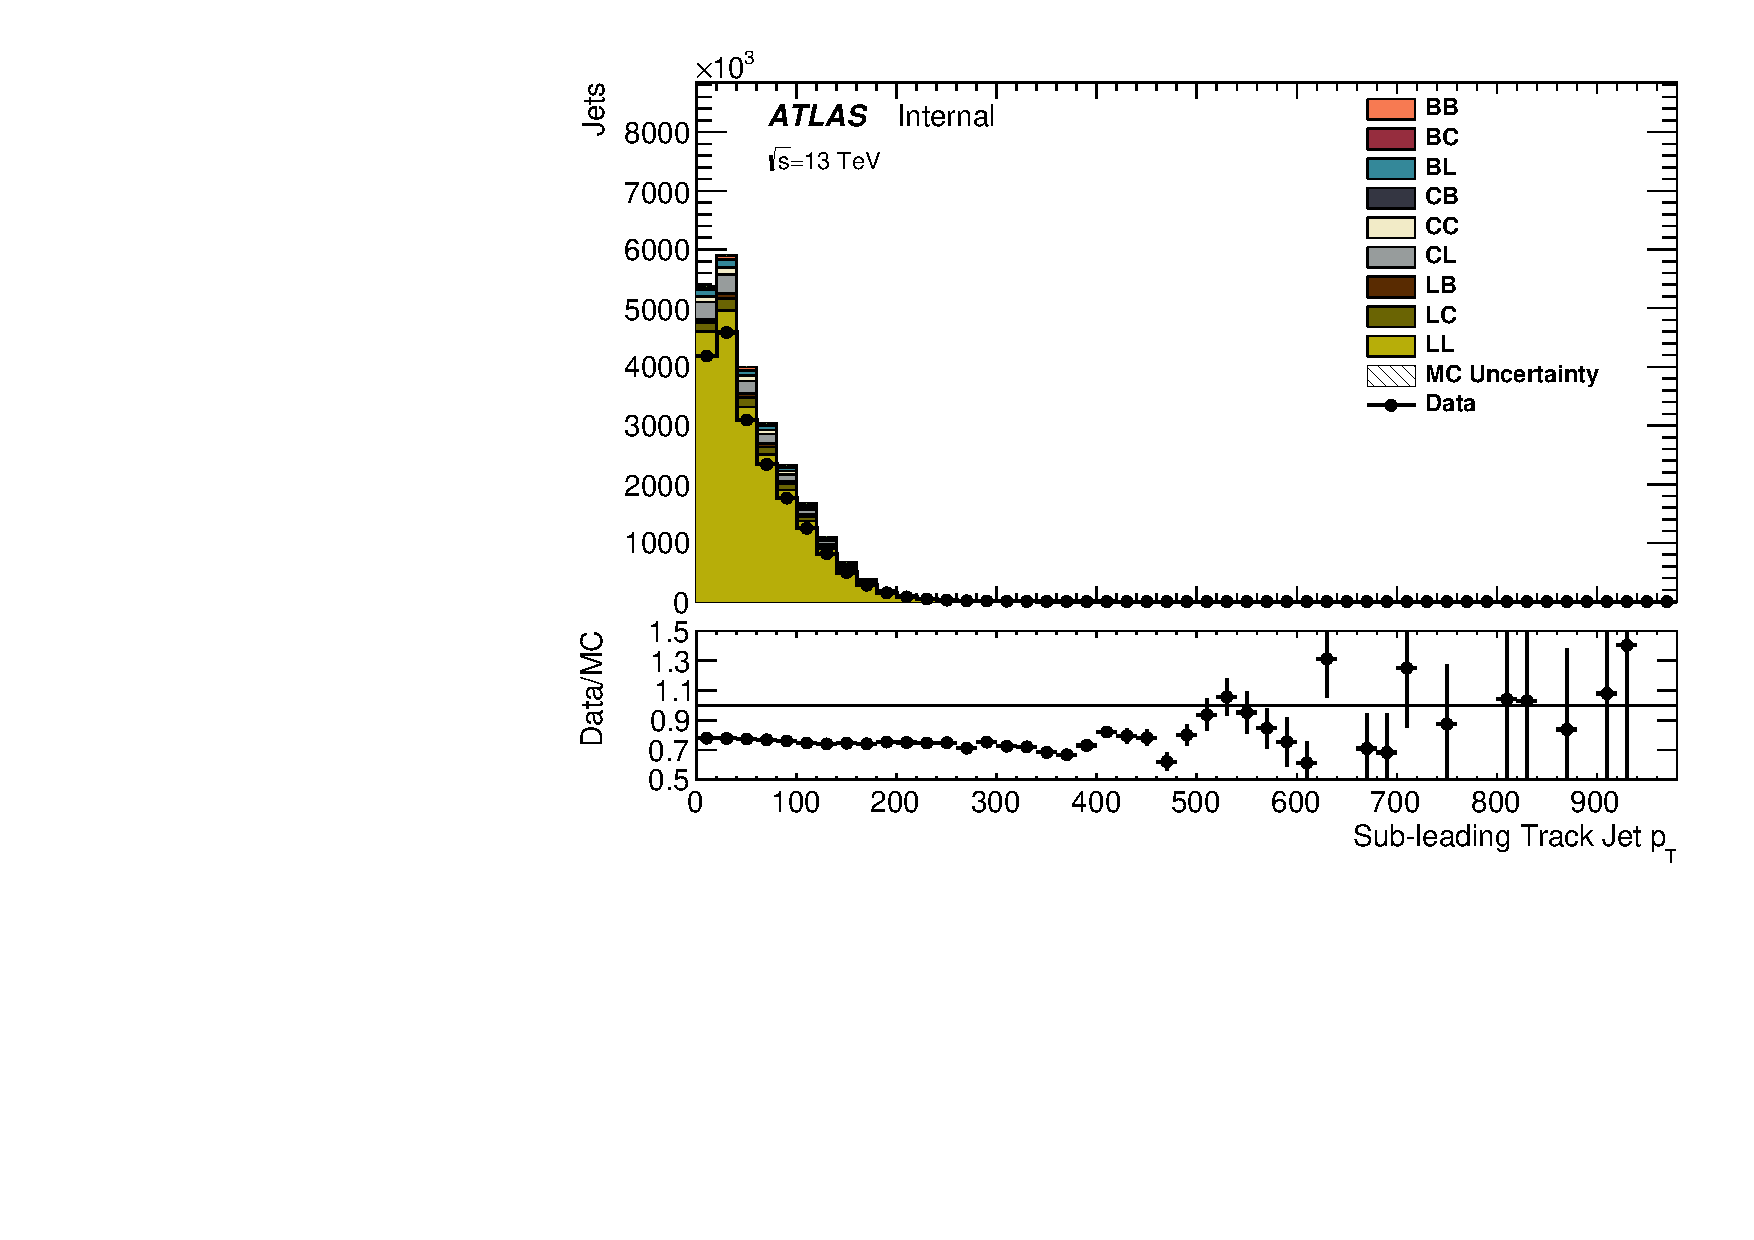
\includegraphics[width=0.45\textwidth]{figures/gbb/SubLeadTrkJet_pT_NoReweight.pdf}
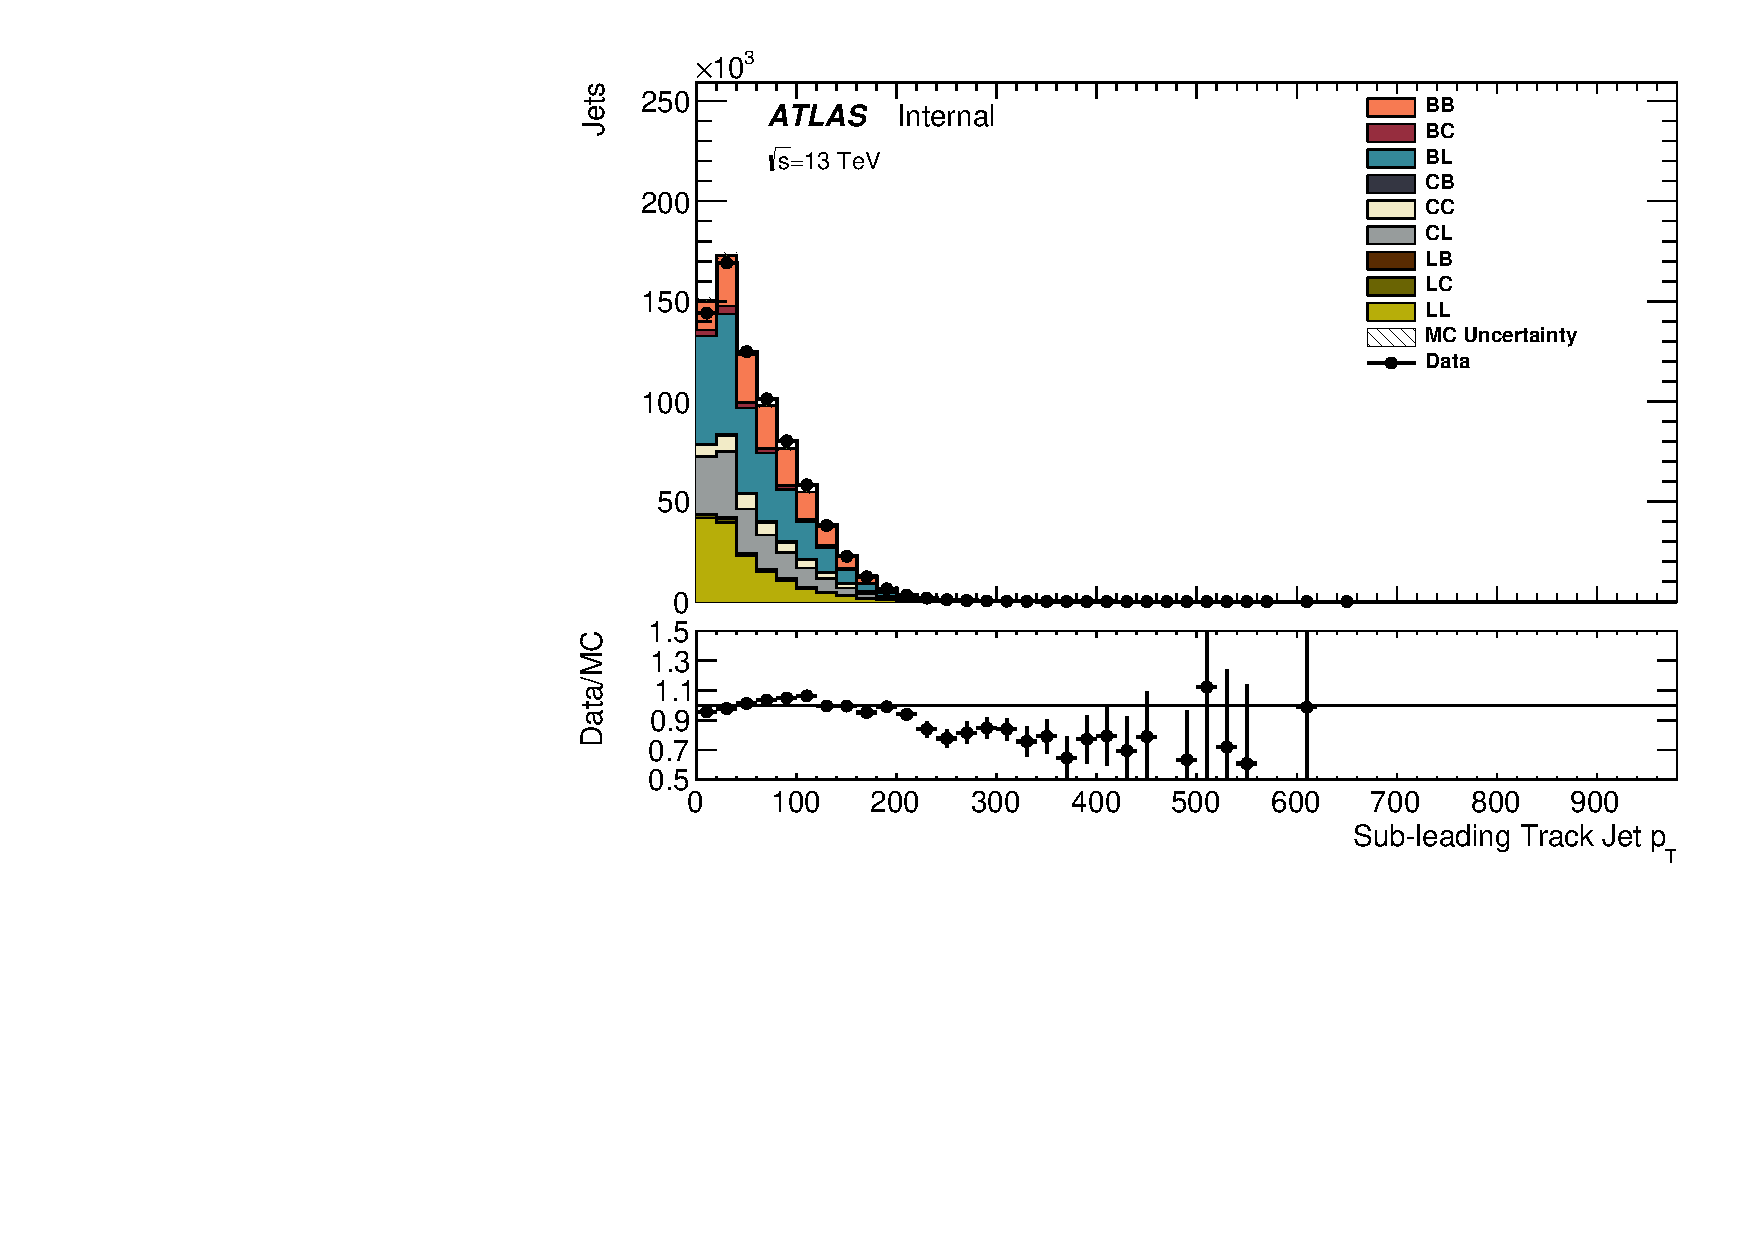
\includegraphics[width=0.45\textwidth]{figures/gbb/SubLeadTrkJet_pT_PreReweight.pdf}\\
 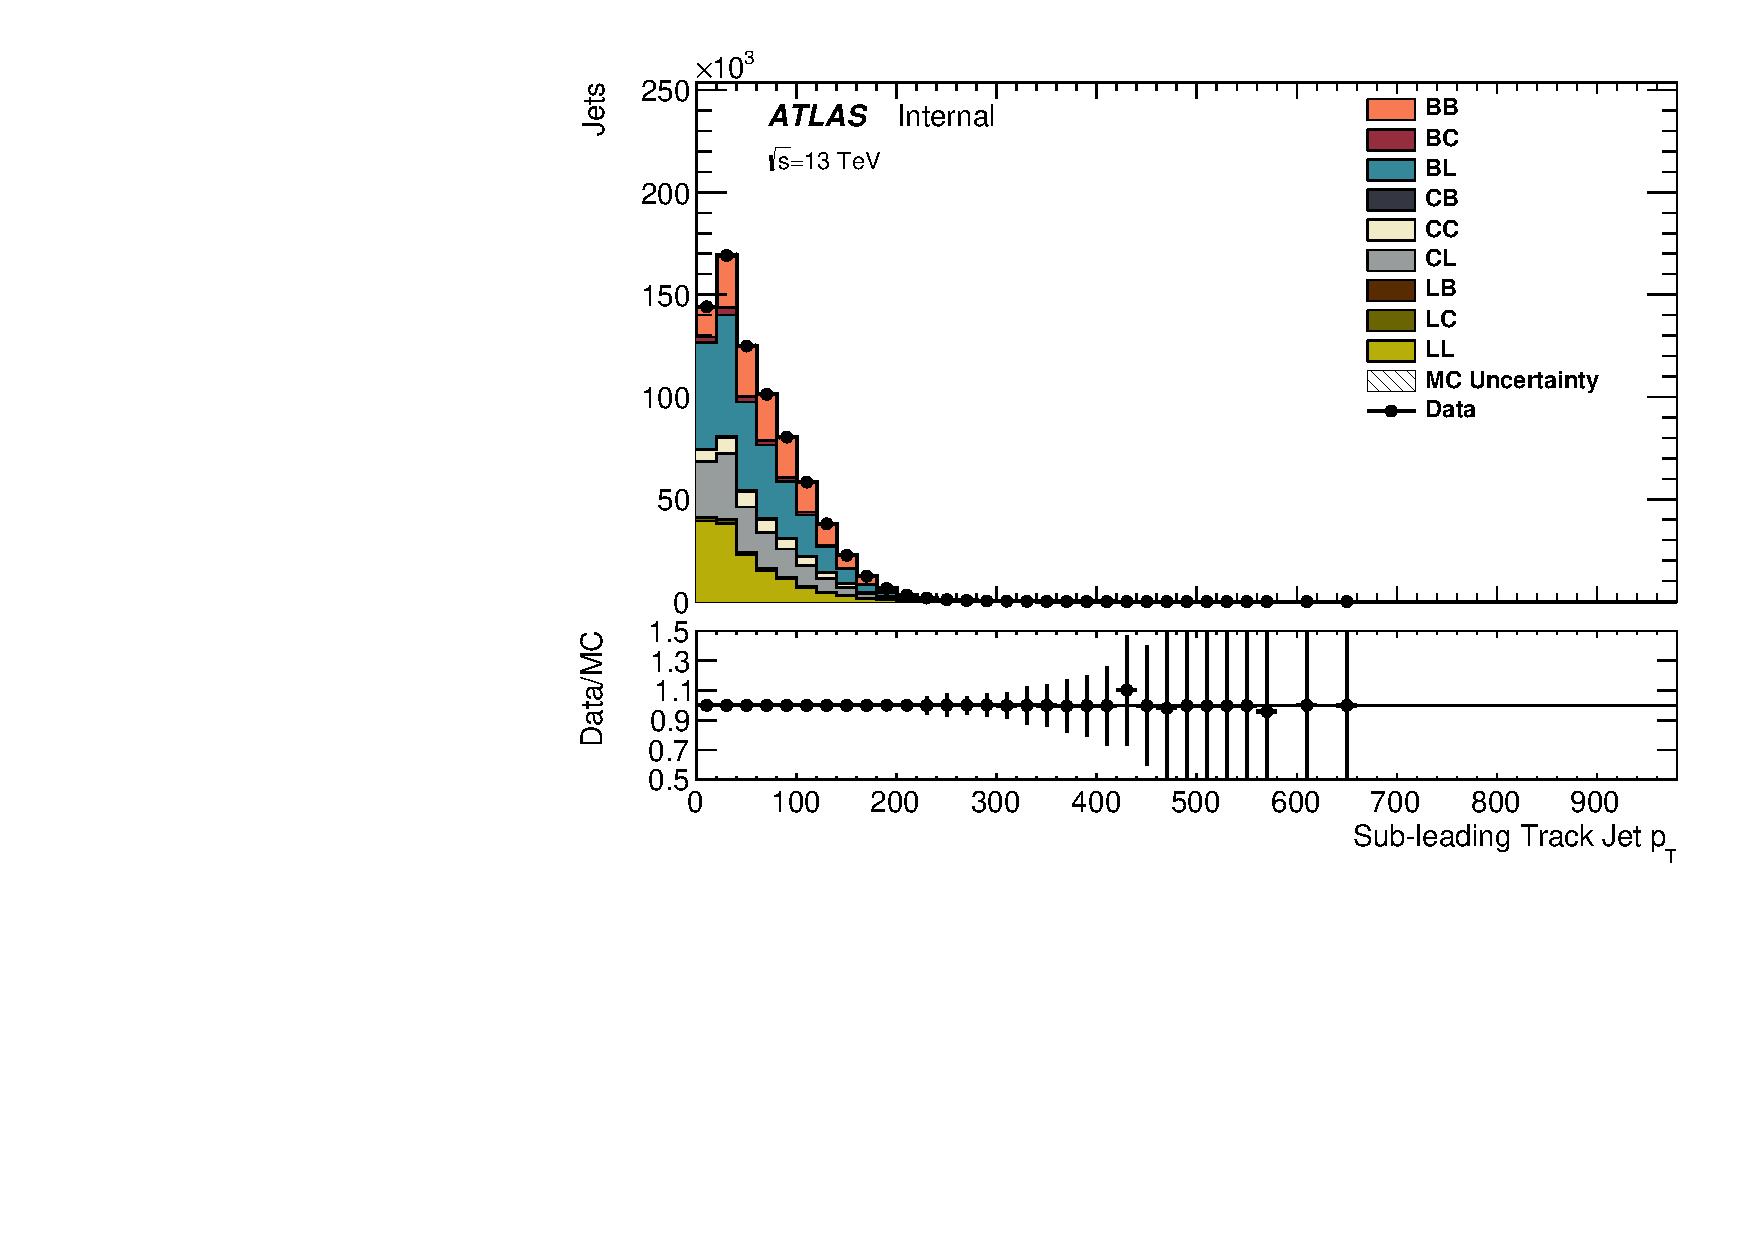
\includegraphics[width=0.45\textwidth]{figures/gbb/SubLeadTrkJet_pT_Reweight.pdf}
\caption{Data/MC comparison of sub-leading track jets $p_T$ before applying $b$-tagging (top left), post $b$-tagging without kinematic reweighting (top right) and post $b$-tagging with kinematic reweighting (bottom). The label of the $R=1.0$ jet flavor content ``XY'' denotes the leading and sub-leading track jet flavor. For example, the flavors of the leading and sub-leading track jet of a ``BL'' $R=1.0$ jet are `B' and `Light' respectively.}
  \label{fig:gbb-pT_subtrkjets}
\end{figure}


\begin{figure}[htbp]
  \centering
 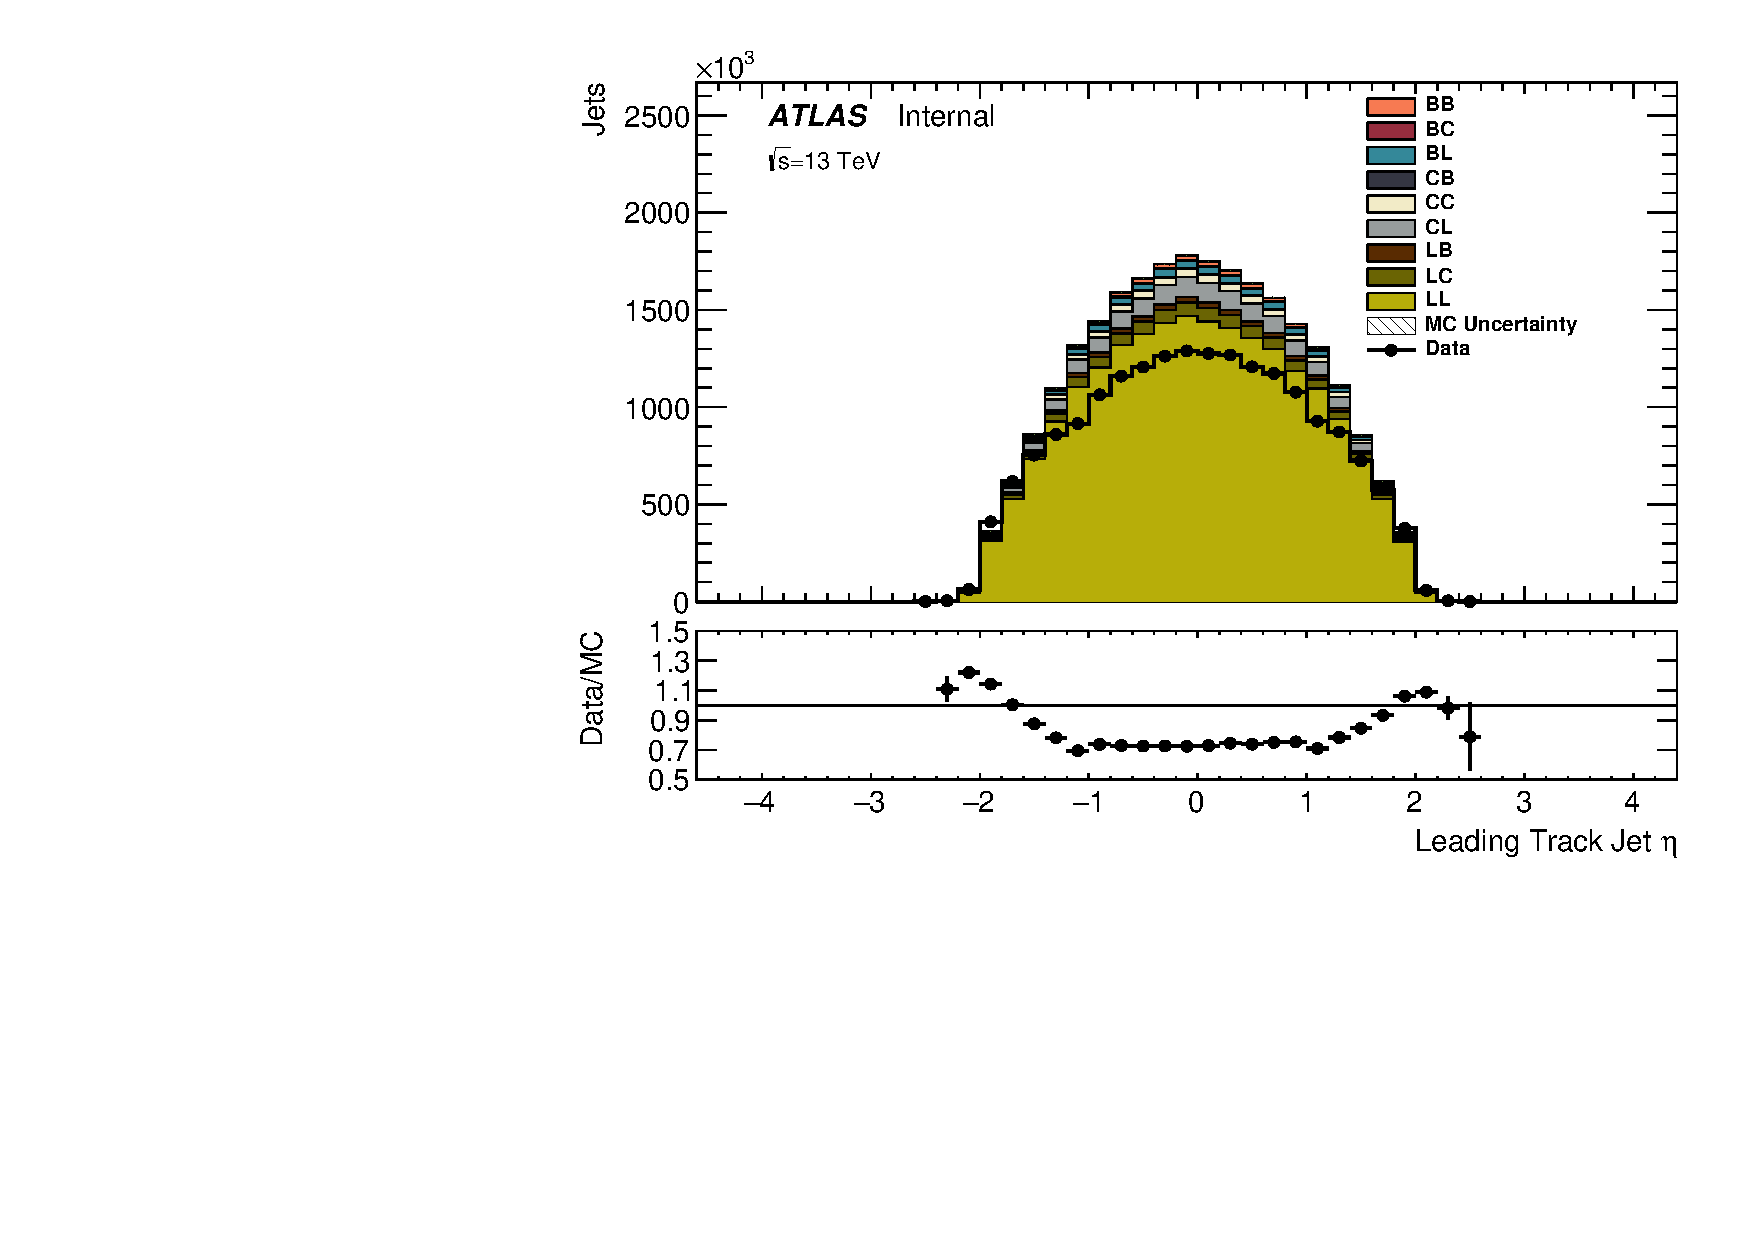
\includegraphics[width=0.45\textwidth]{figures/gbb/LeadTrkJet_eta_NoReweight.pdf}
 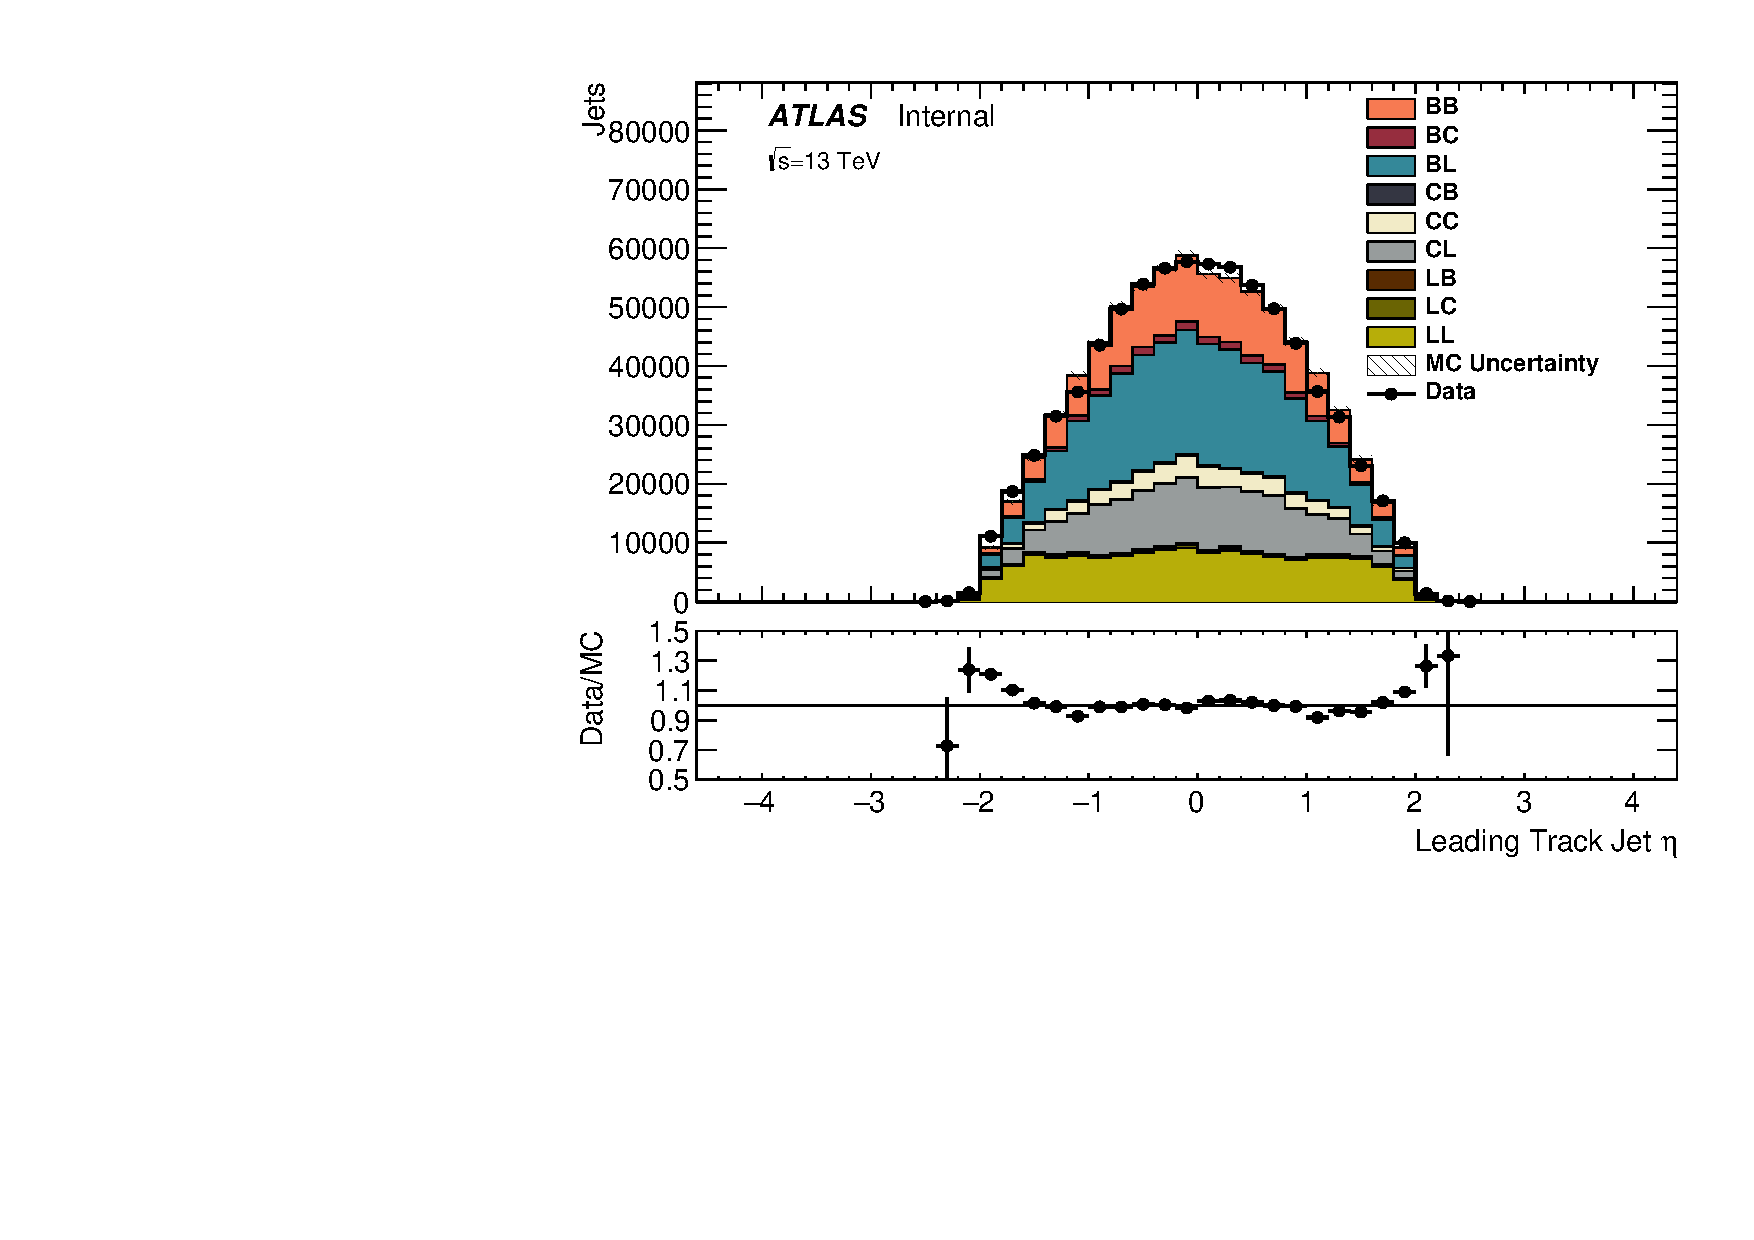
\includegraphics[width=0.45\textwidth]{figures/gbb/LeadTrkJet_eta_PreReweight.pdf}\\
 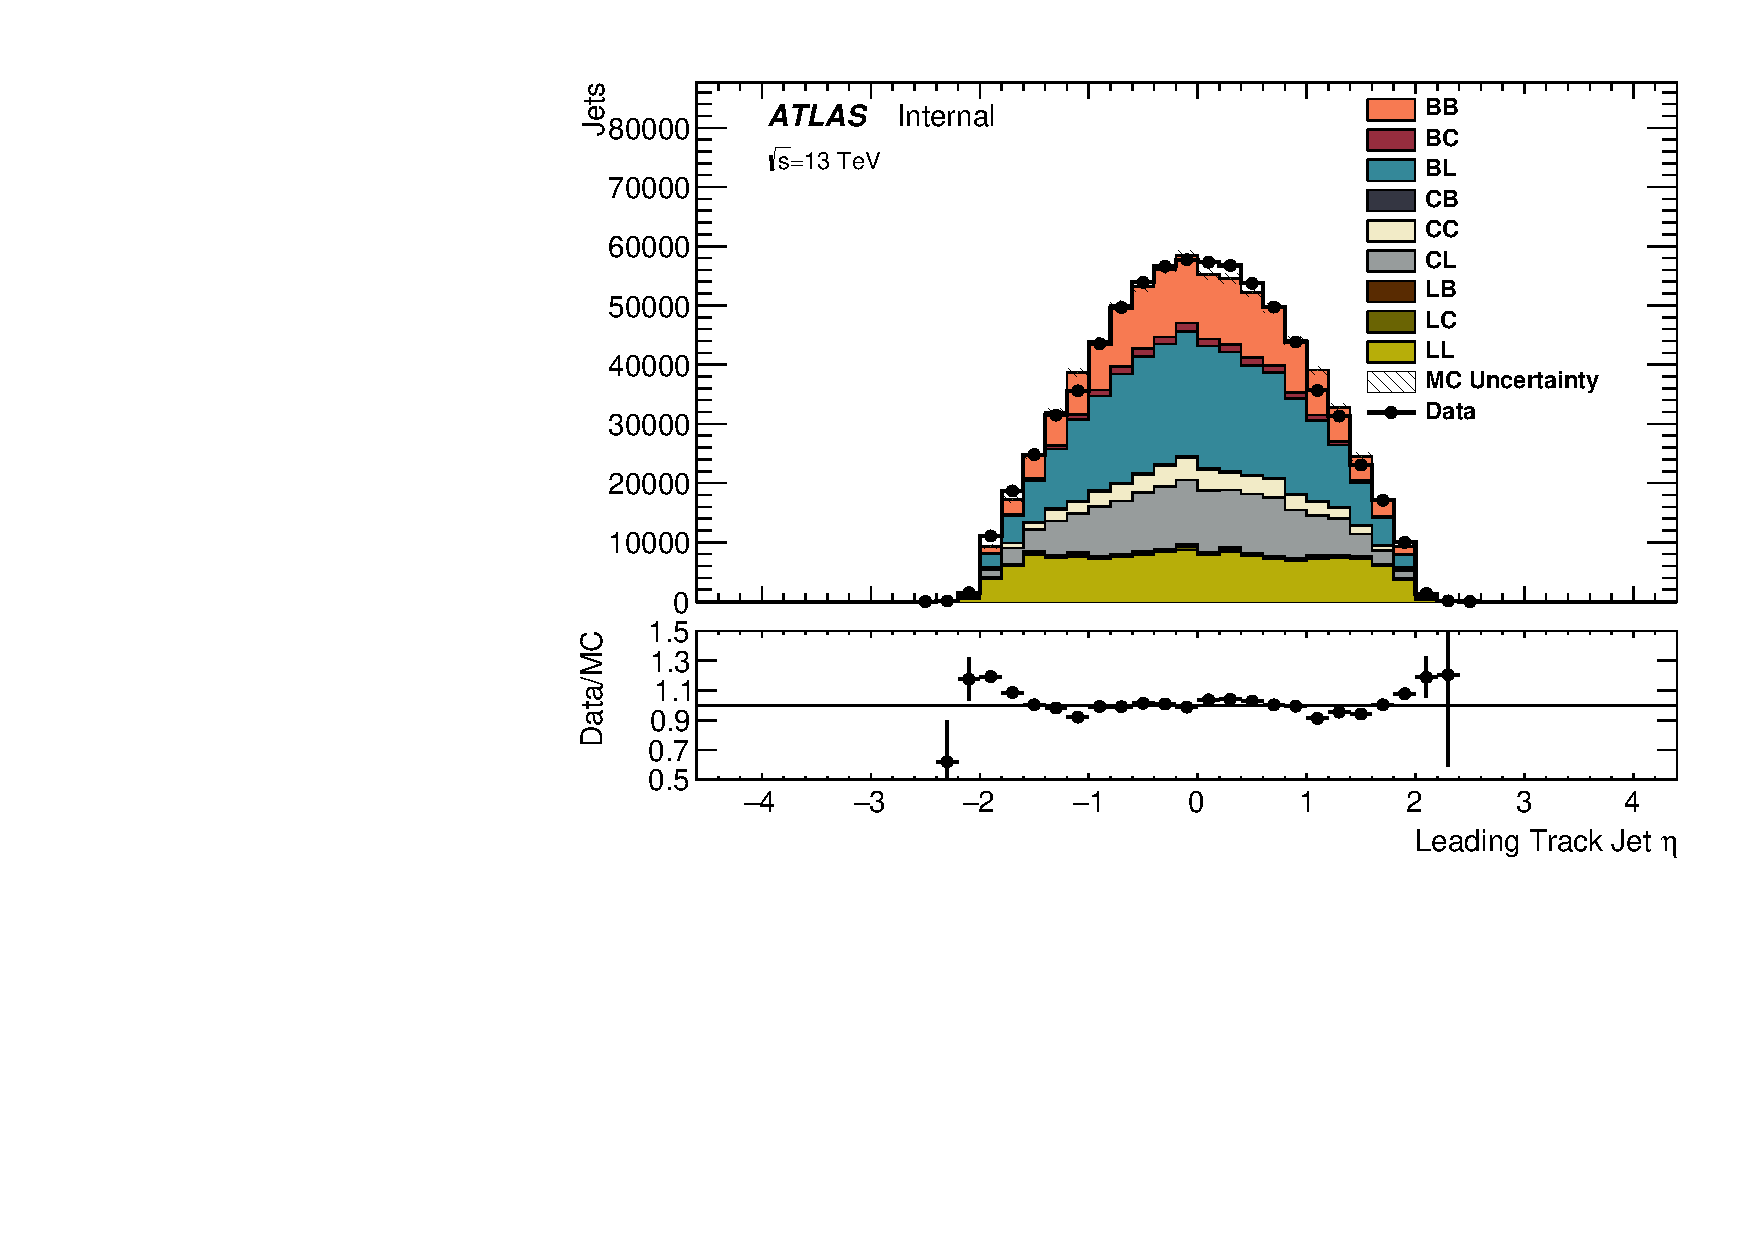
\includegraphics[width=0.45\textwidth]{figures/gbb/LeadTrkJet_eta_Reweight.pdf}
\caption{Data/MC comparison of leading track jets $\eta$ before applying $b$-tagging (top left), post $b$-tagging without kinematic reweighting (top right) and post $b$-tagging with kinematic reweighting (bottom). The label of the $R=1.0$ jet flavor content ``XY'' denotes the leading and sub-leading track jet flavor. For example, the flavors of the leading and sub-leading track jet of a ``BL'' $R=1.0$ jet are `B' and `Light' respectively.}
  \label{fig:gbb-eta_leadtrkjets}
\end{figure}


\begin{figure}[htbp]
  \centering
 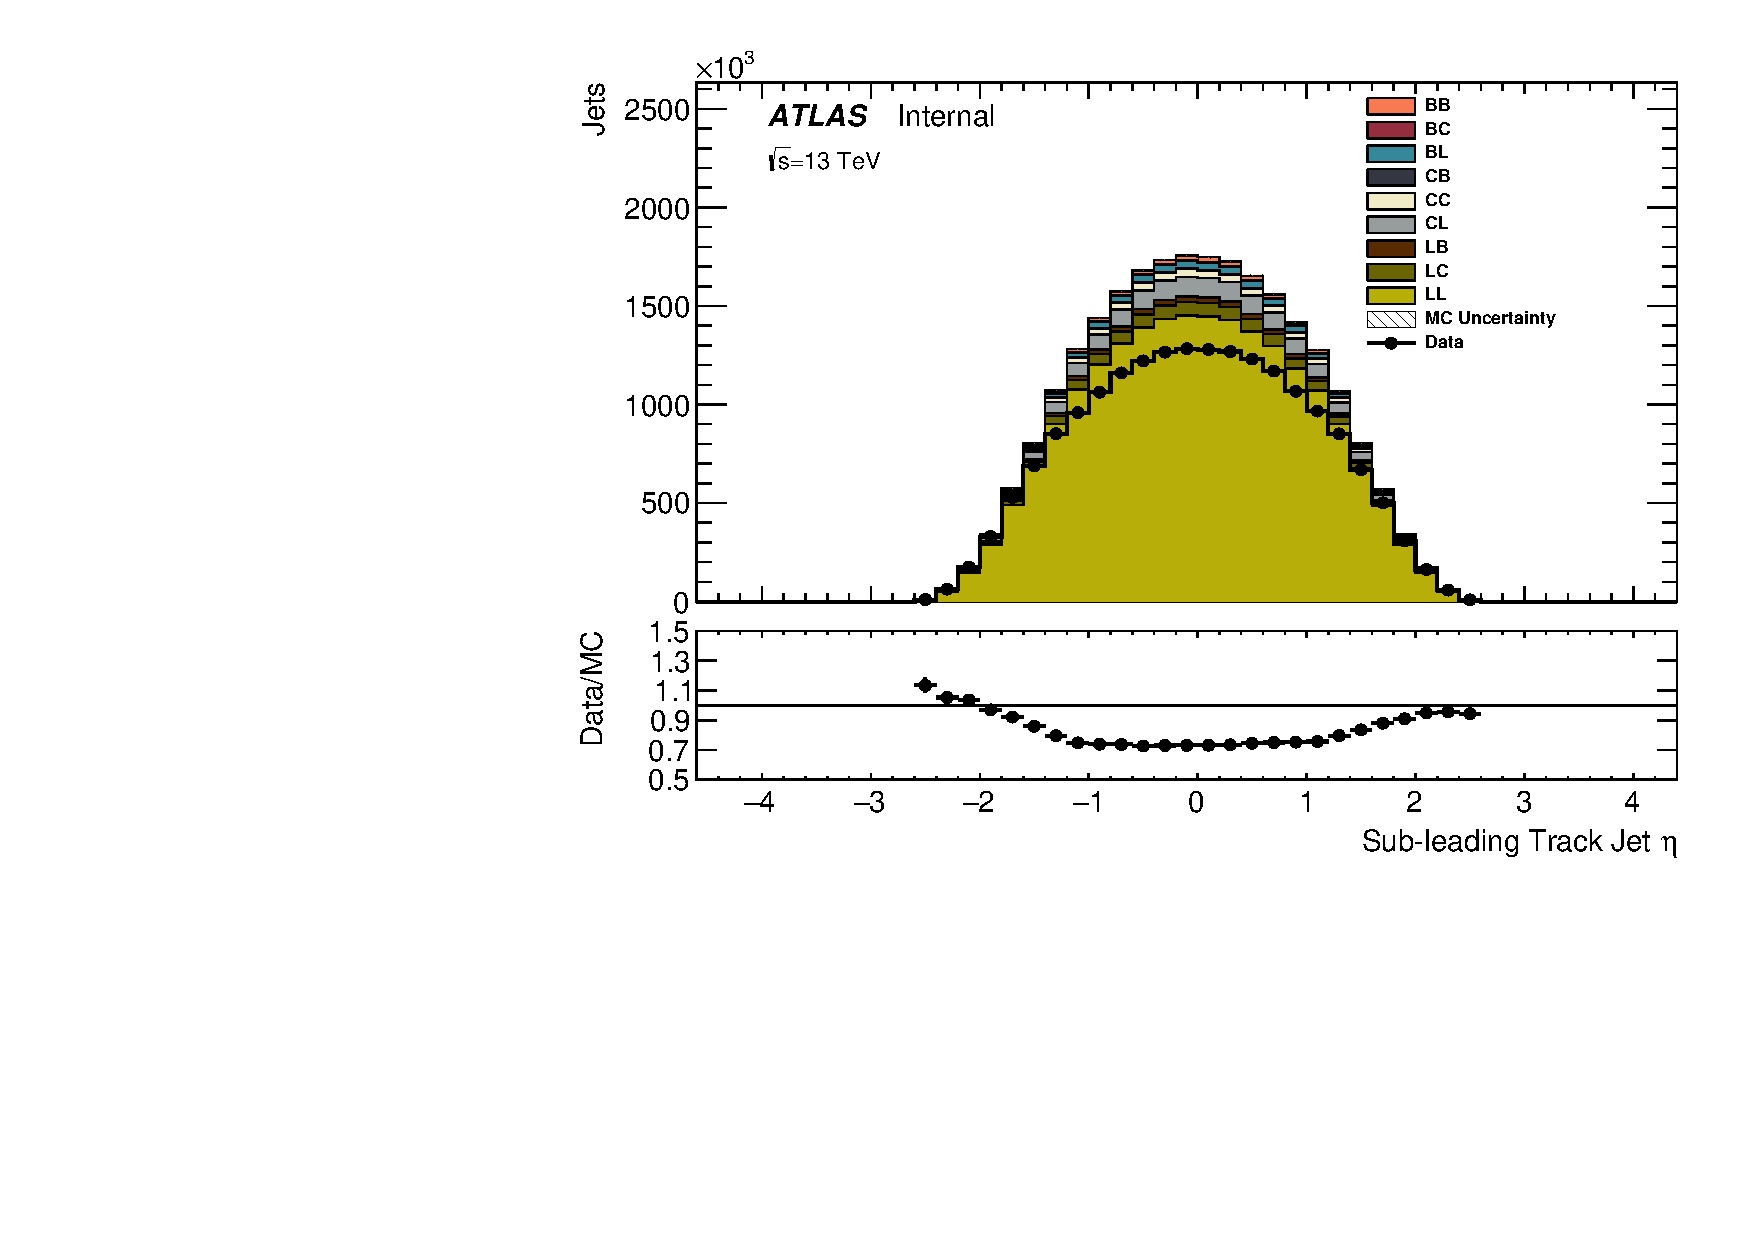
\includegraphics[width=0.45\textwidth]{figures/gbb/SubLeadTrkJet_eta_NoReweight.pdf}
 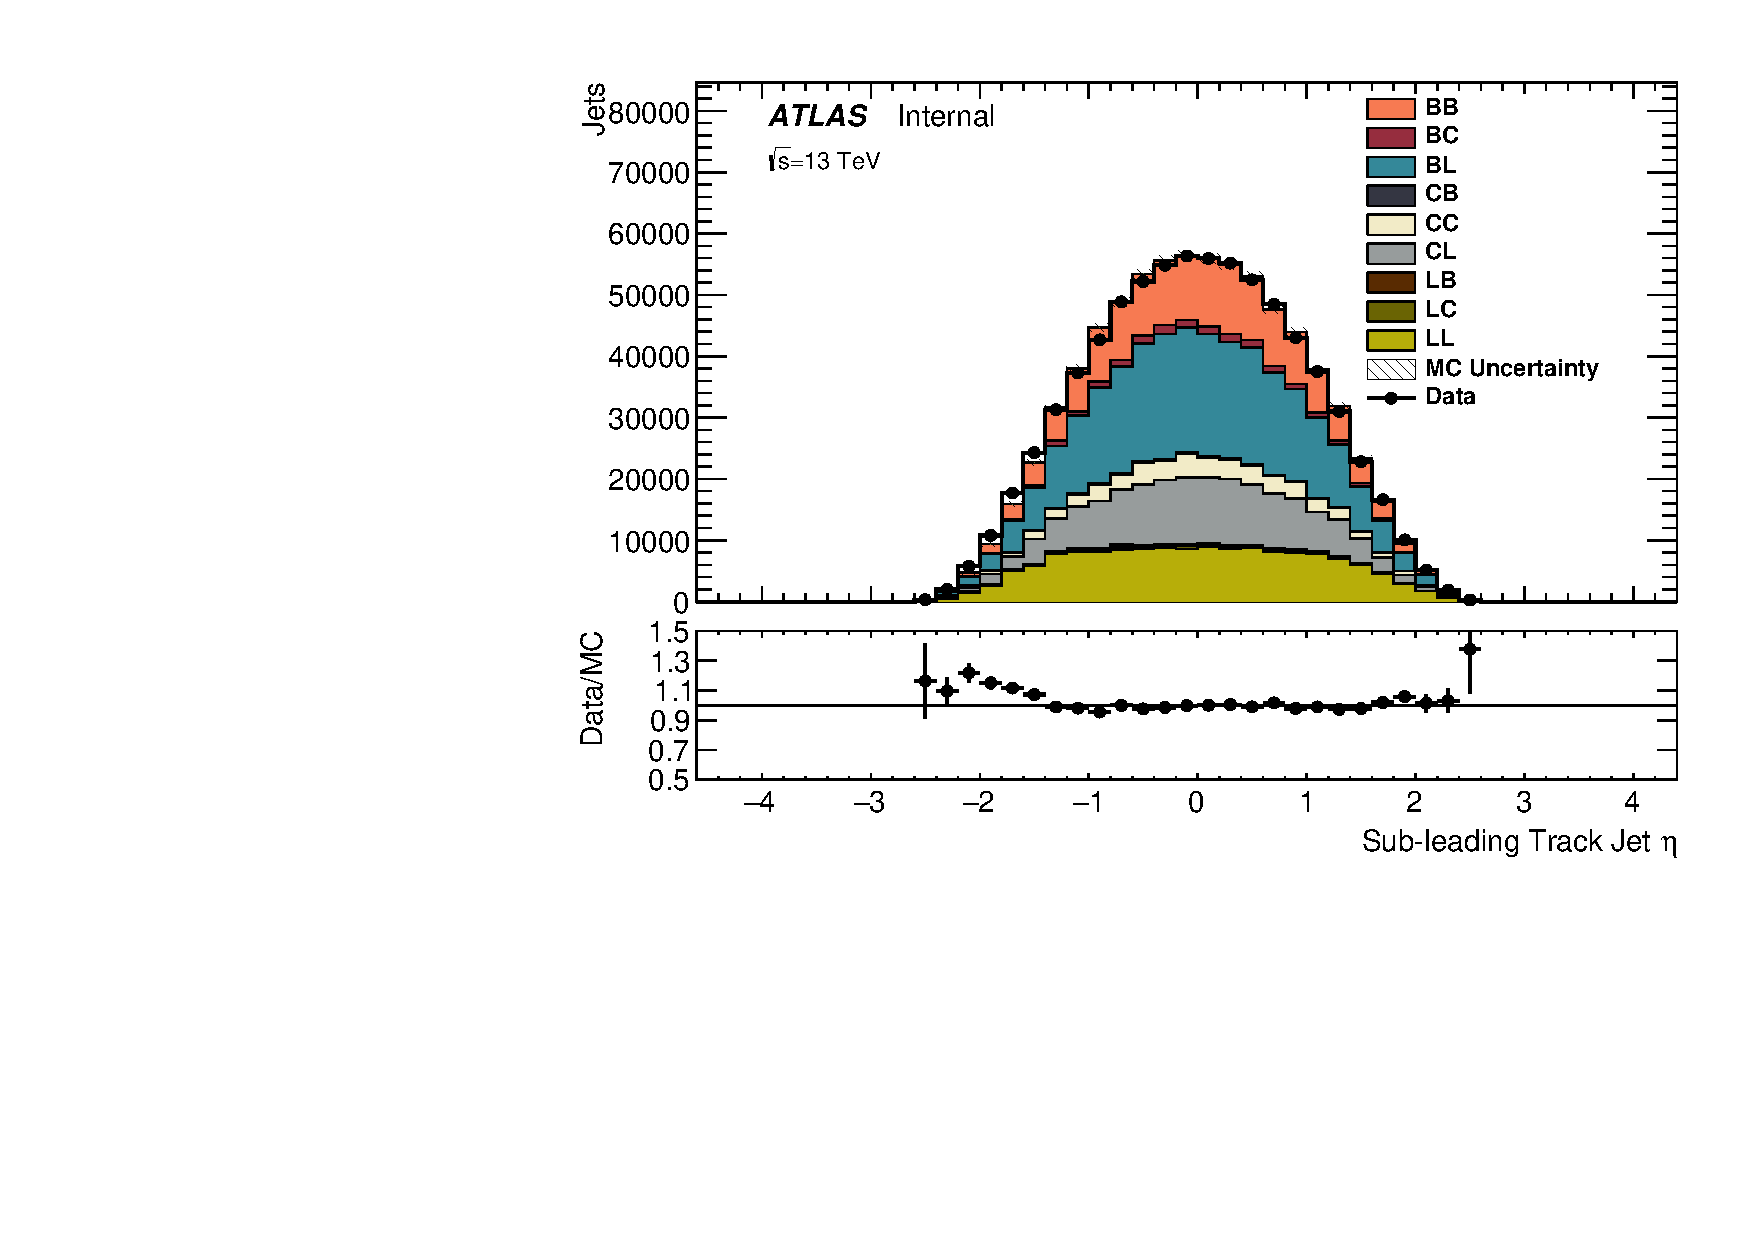
\includegraphics[width=0.45\textwidth]{figures/gbb/SubLeadTrkJet_eta_PreReweight.pdf}\\
 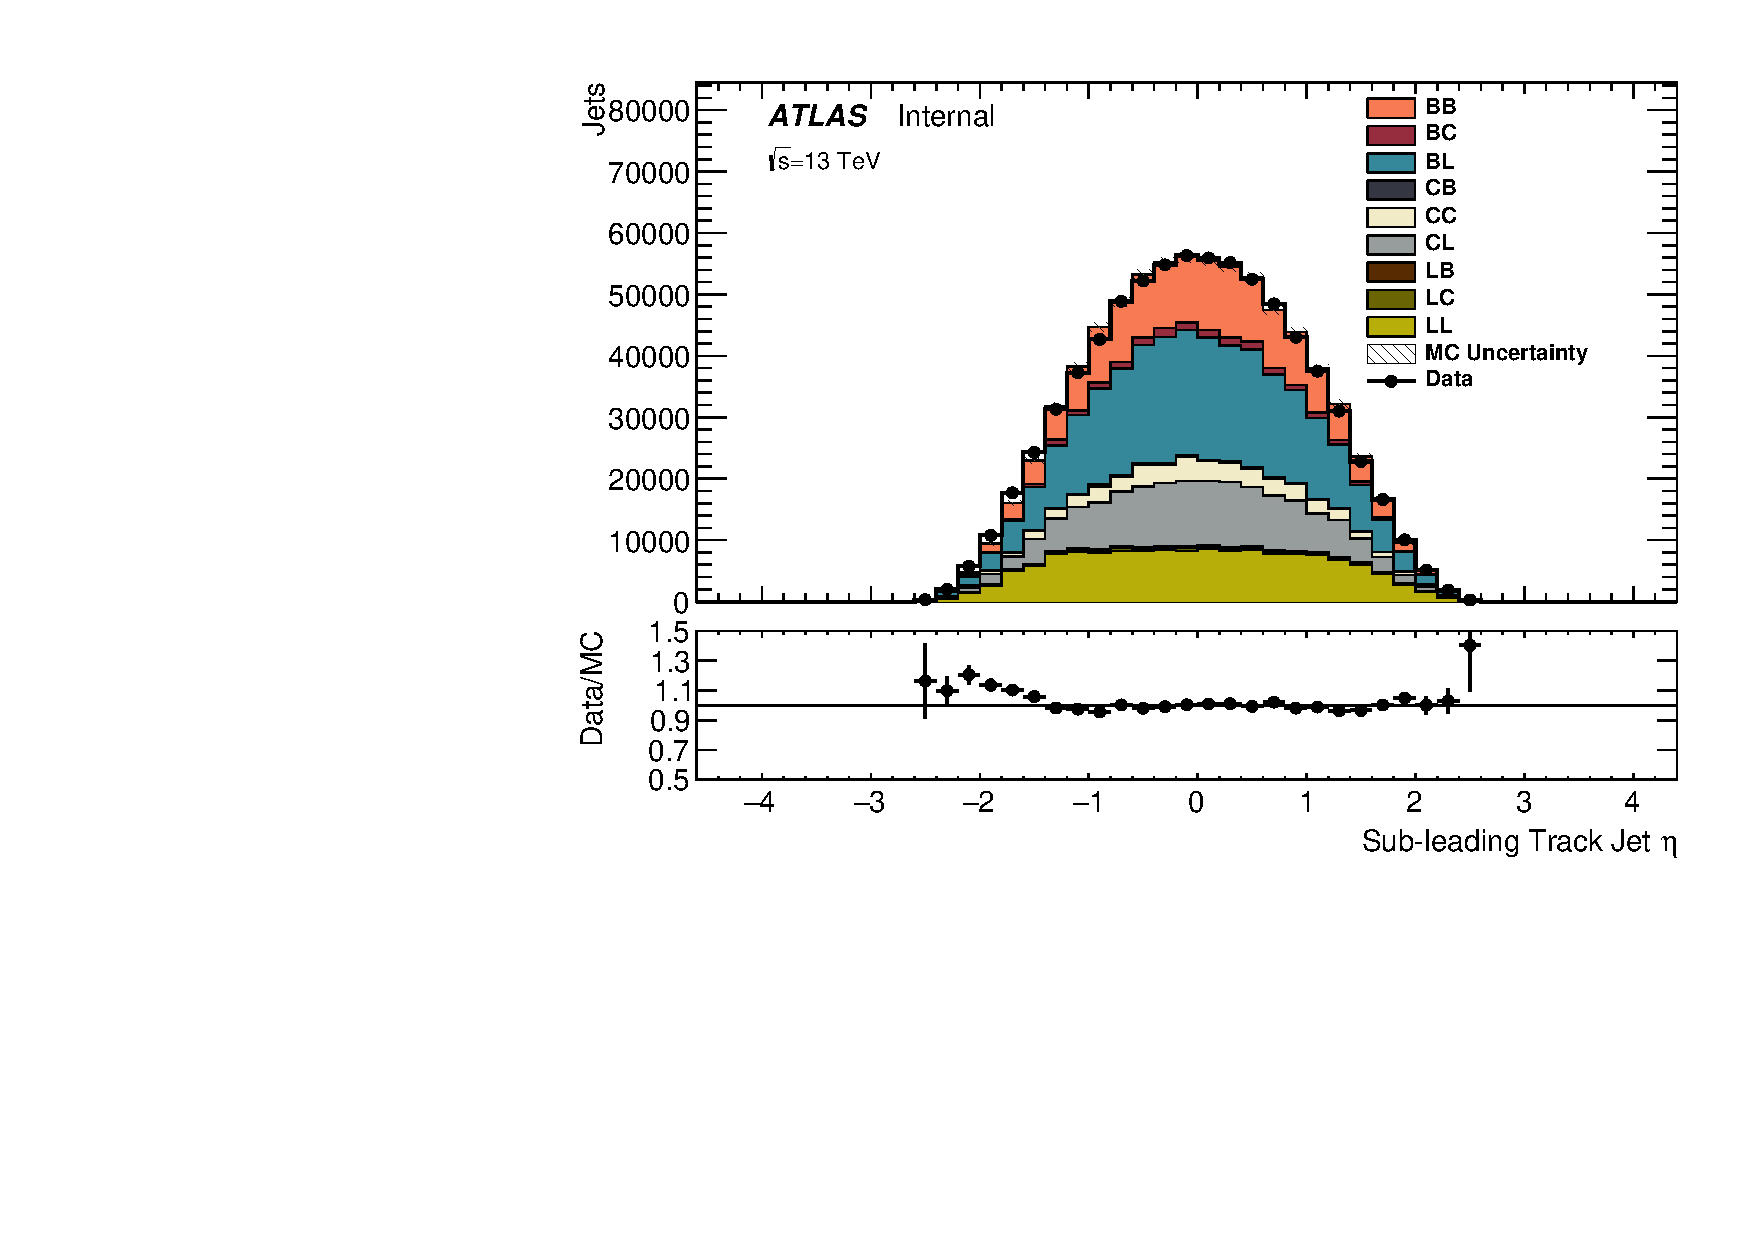
\includegraphics[width=0.45\textwidth]{figures/gbb/SubLeadTrkJet_eta_Reweight.pdf}
\caption{Data/MC comparison of sub-leading track jets $\eta$ before applying $b$-tagging (top left), post $b$-tagging without kinematic reweighting (top right) and post $b$-tagging with kinematic reweighting (bottom). The label of the $R=1.0$ jet flavor content ``XY'' denotes the leading and sub-leading track jet flavor. For example, the flavors of the leading and sub-leading track jet of a ``BL'' $R=1.0$ jet are `B' and `Light' respectively.}
  \label{fig:gbb-eta_subtrkjets}
\end{figure}




\clearpage

%-------------------------------------------------------------------------------
\section{Observables}
\label{sec:variables}
%-------------------------------------------------------------------------------
There are\footnote{This section is stolen from Ref.~\cite{Ilten:2017rbd} and has benefited from conversations with Peter Skands.} several aspects of the $g\rightarrow b\bar{b}$ decay that would provide nearly direct measurements of the fragmentation function.  Three key variables are\footnote{Plots for the unnormalized mass can be found in Appendix~\ref{sec:app-trkmass}.} $\Delta R(b,\bar{b}), \rho_{b\bar{b}}=m_{b\bar{b}}/p_\text{T,$b\bar{b}$}$, and $z_{b\bar{b}}=p_\text{b}/p_\text{T,g}$.  None of the distributions of these quantities have been measured for $\Delta R(b,\bar{b}) < R$ ($R=$ jet radius).  Figure~\ref{fig:gbb-gbbdistributions} shows the distribution of these three variables, as predicted by Pythia~\cite{Pythia8}.  In addition to the nominal prediction, the sensitivity to variations in the modeling of fragmentation is illustrated by varying parameters in Pythia~\cite{pythiavariations}.  The variables sensitive to the $b\bar{b}$ opening angle ($\Delta R$ and mass) have 10\% variations due to the scale variations in the fragmentation.  There are likely other variations that these observables are sensitive to, such as the quark mass effects.

One of the key choices in this measurement is deciding to unfold to less observable quantities ($b$-quarks), more observable quantities ($b$-jets or $b$ track-jets), or somewhere in between ($B$-hadrons).  The impact of this choice is illustrated in Fig.~\ref{fig:gbb-gbbresponse}.  For $\Delta R$, all choices give similar answers.  Unsurprisingly, the momentum fraction is more sensitive to the choice of unfolding target.  In order to have access to small angular scales without needing to explicitly reconstruct $B$-hadrons, we use small-radius track jets.

In addition to the QCD properties of the fragmentation, one can also make measurements of observables that are sensitive to the gluon spin, as in the angle between the gluon production and gluon `decay' planes shown in Fig.~\ref{fig:gbb-gbbangle}.

\begin{figure}[htpb!]
\begin{center}
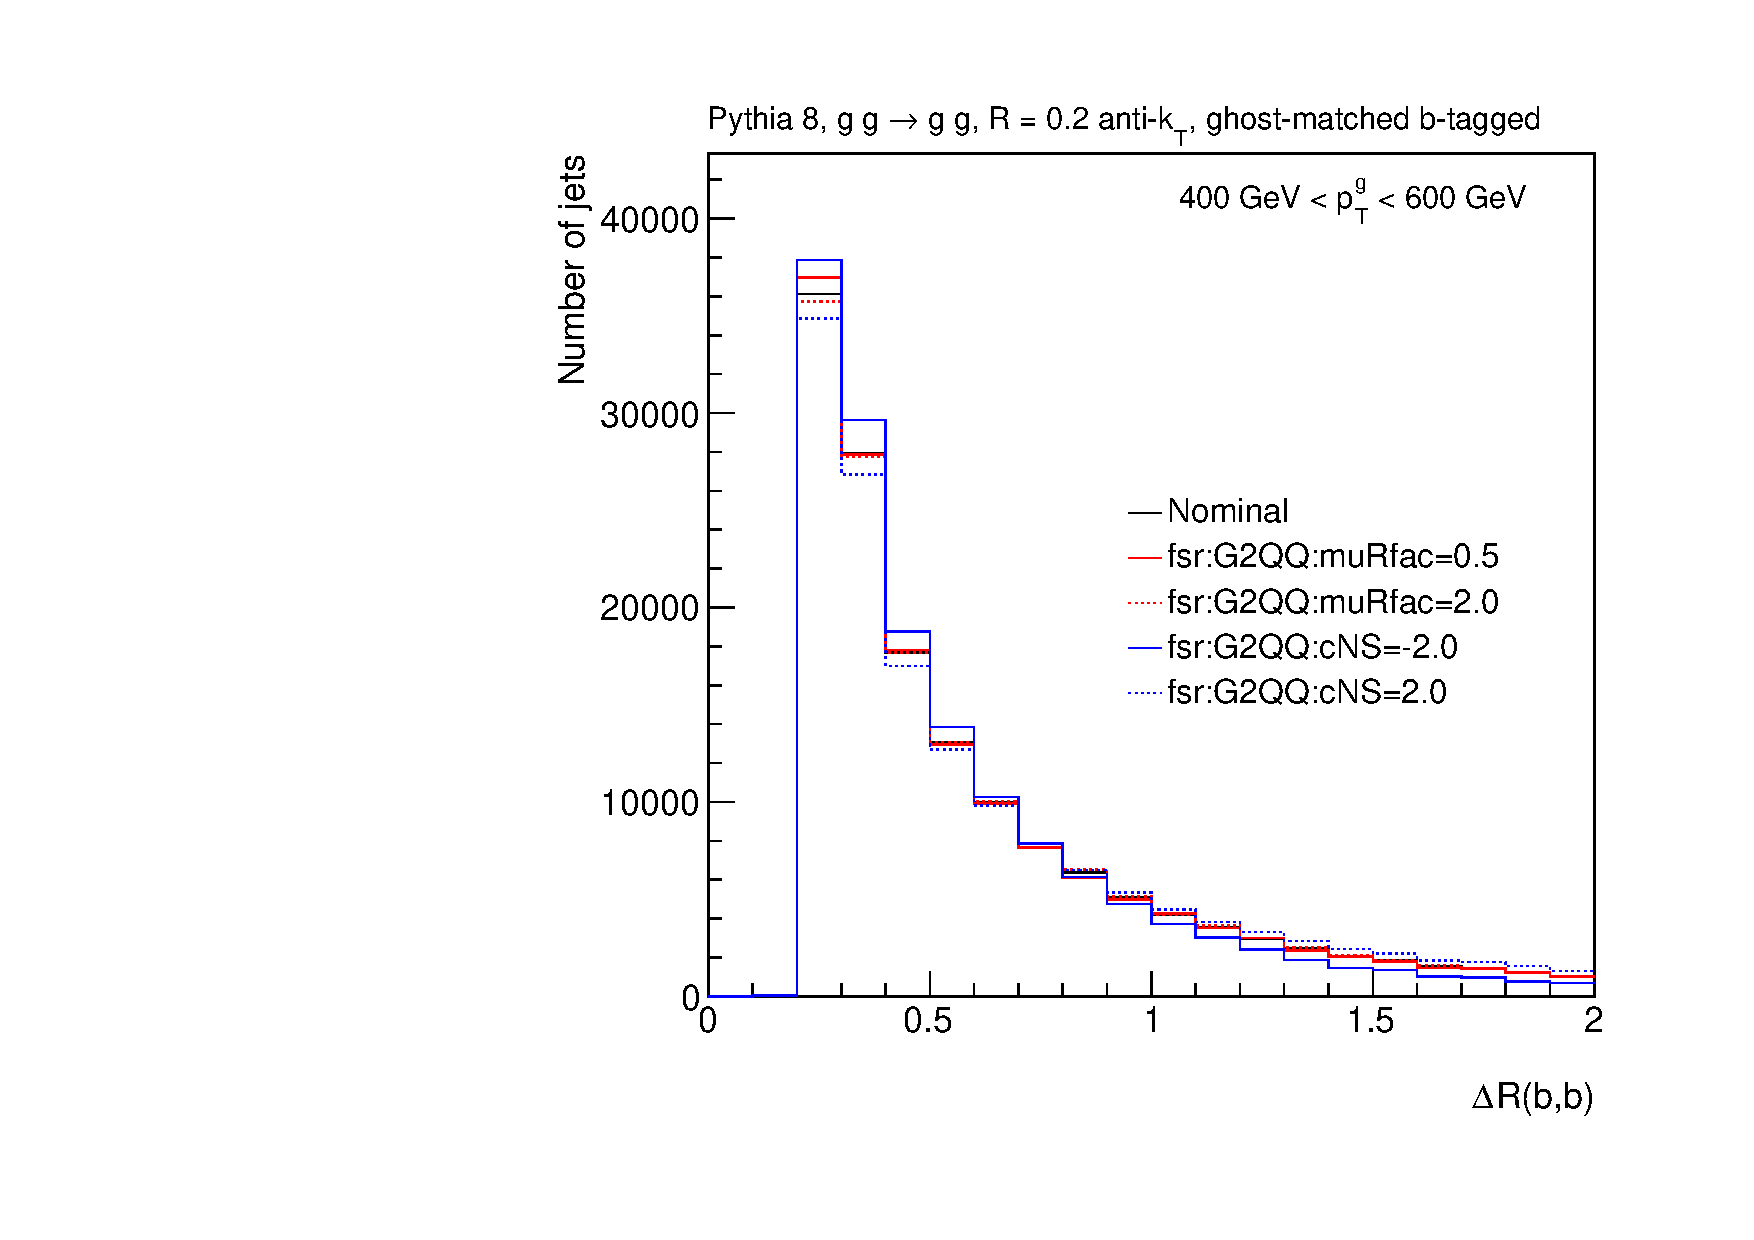
\includegraphics[width=0.33\linewidth]{figures/gbb/truth_level/DeltaRbb.pdf}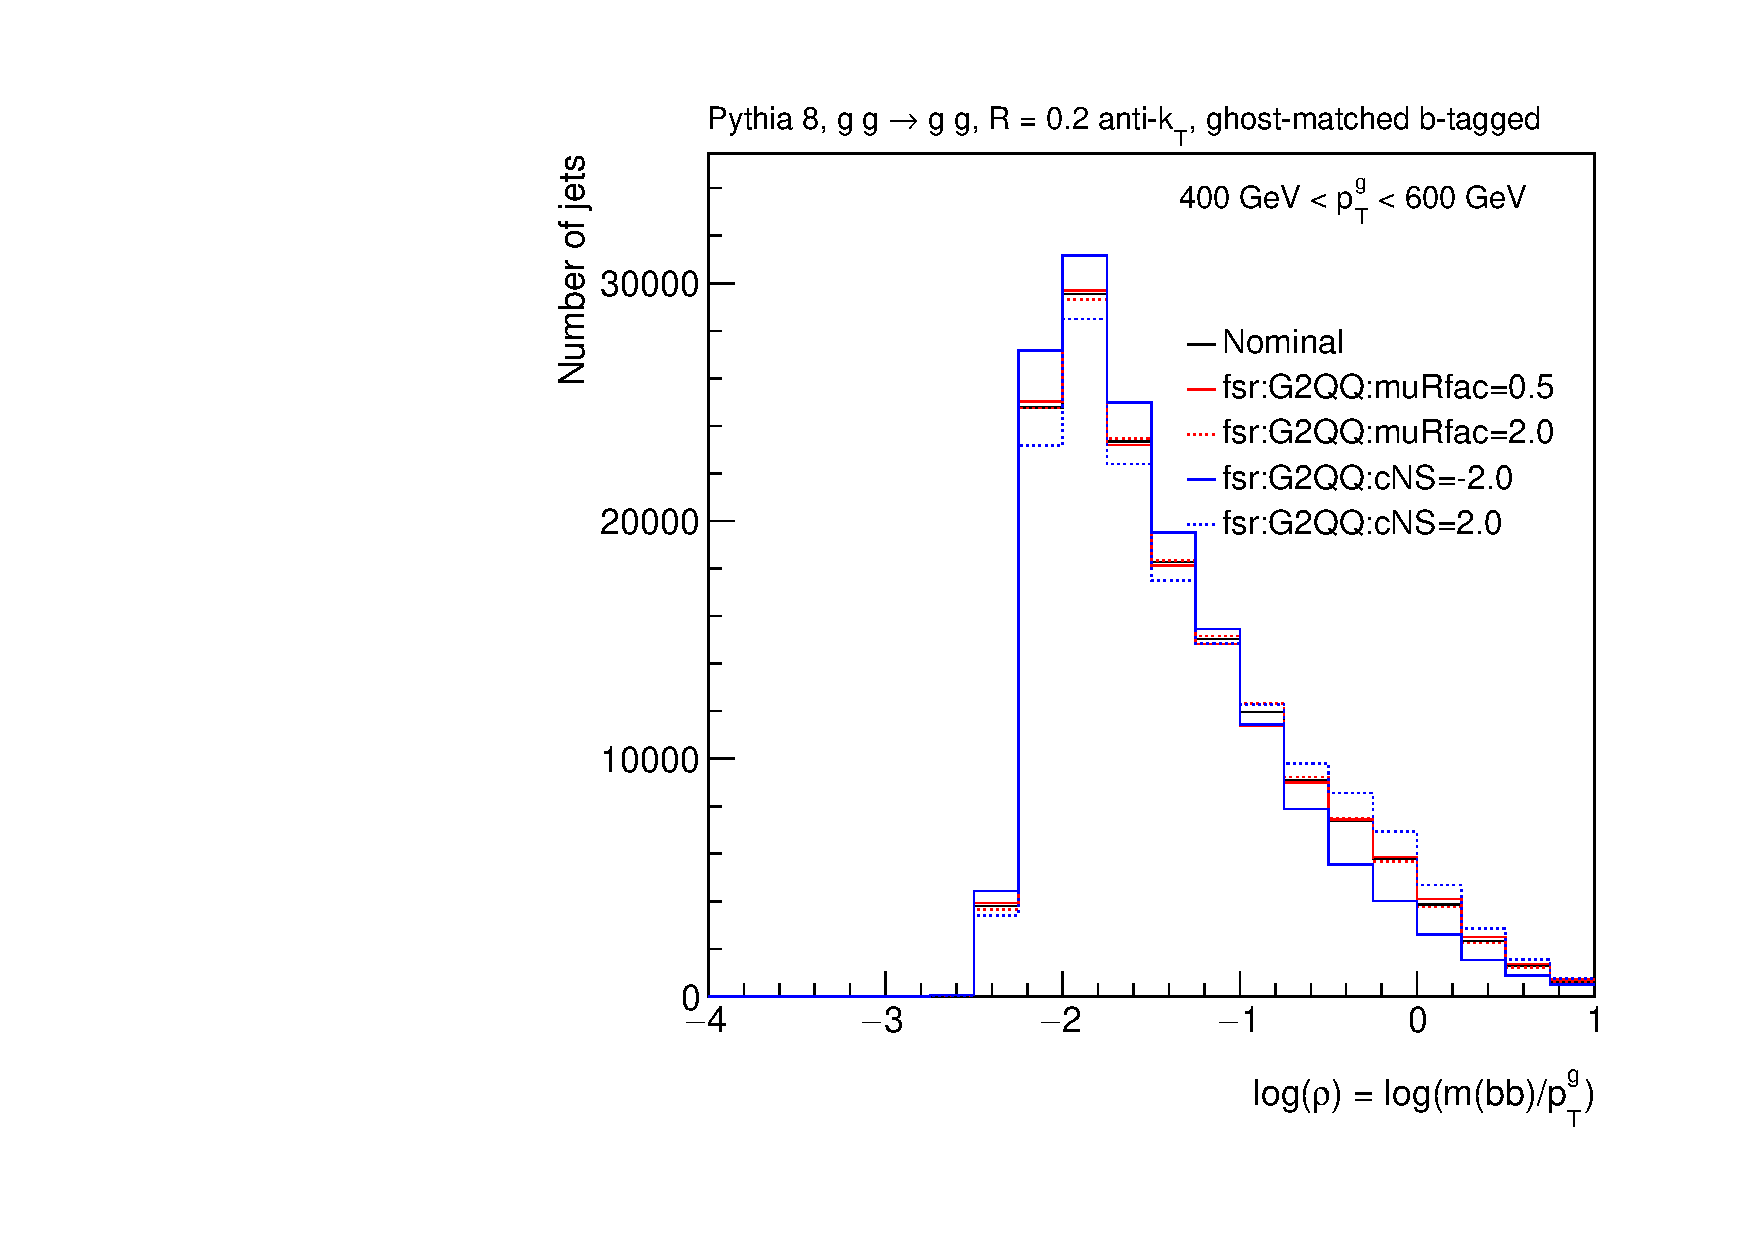
\includegraphics[width=0.33\linewidth]{figures/gbb/truth_level/rhobb.pdf}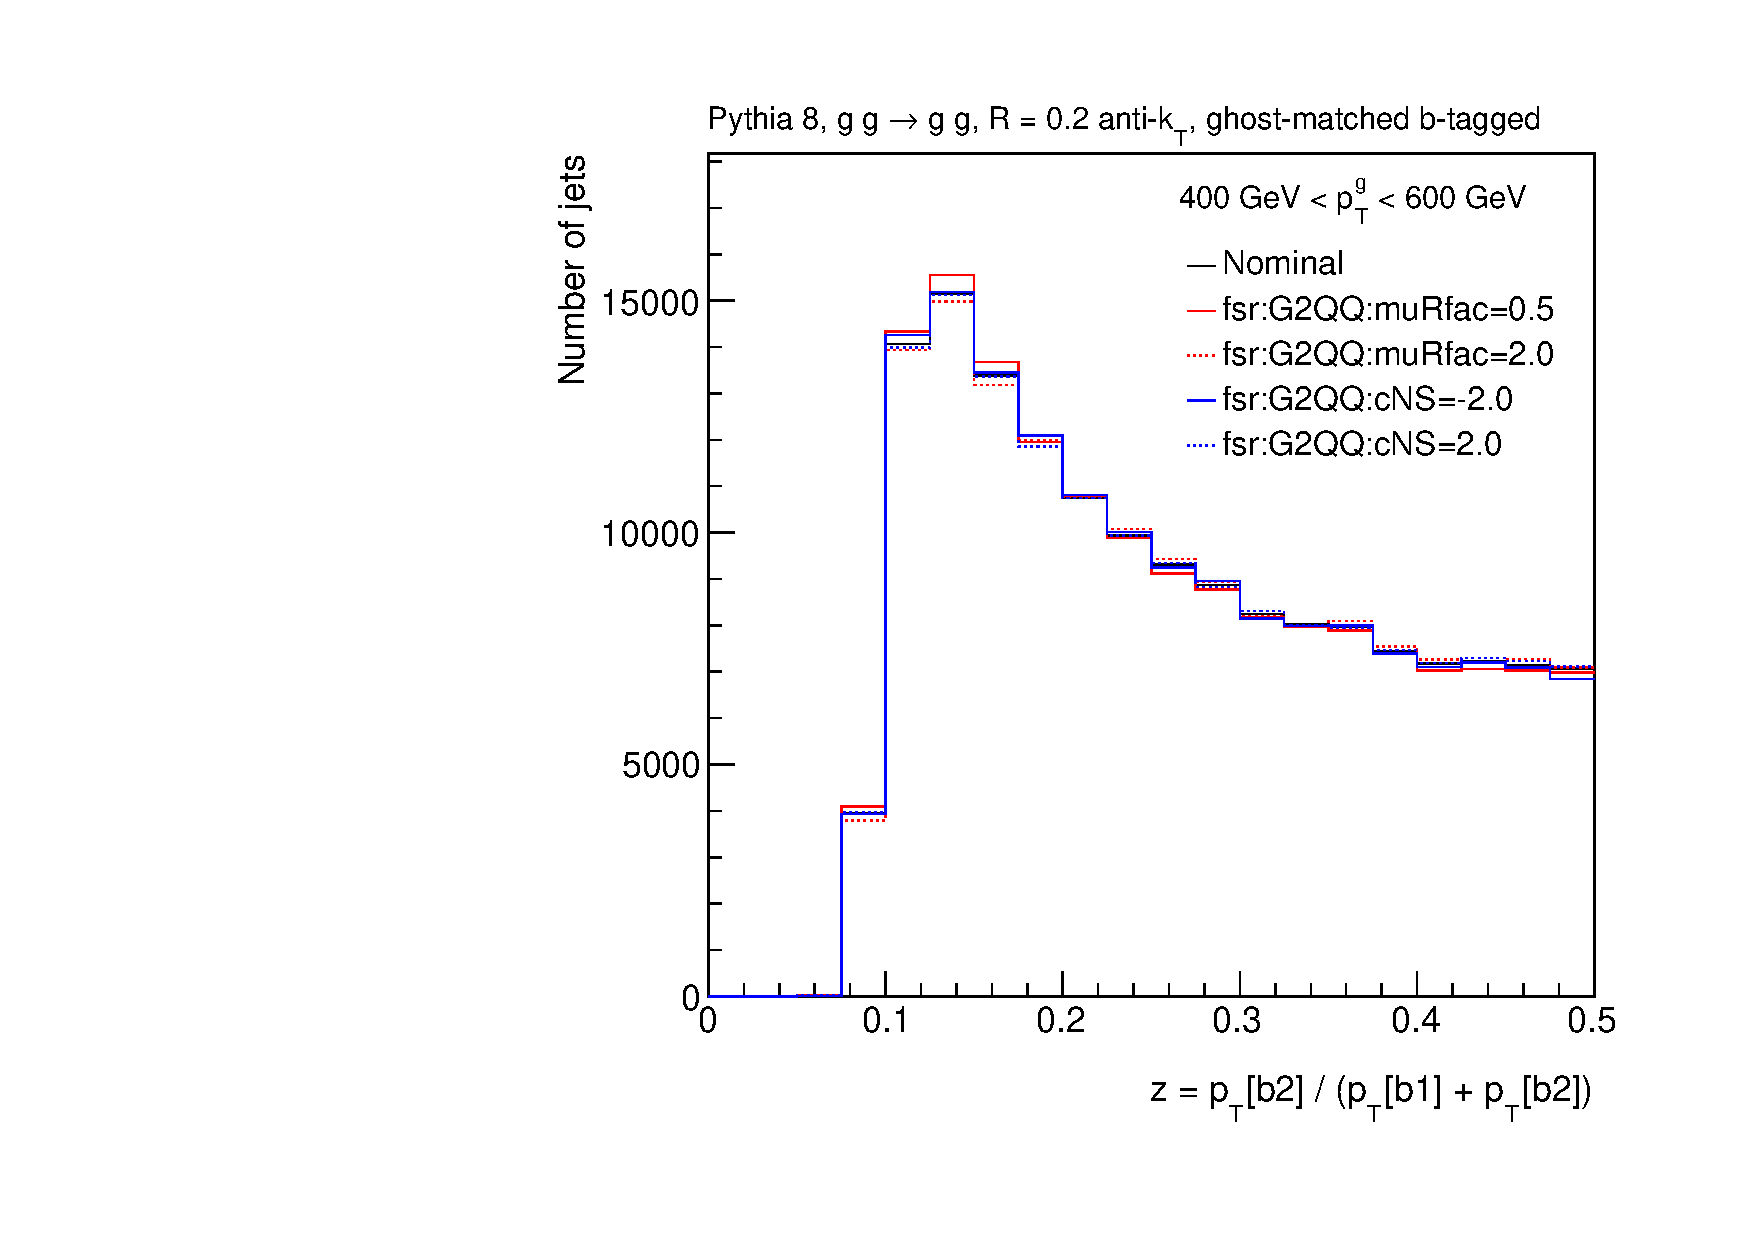
\includegraphics[width=0.33\linewidth]{figures/gbb/truth_level/DeltaZbb.pdf}
\caption{The distributions of $\Delta R(b,\bar{b}), \rho_{b\bar{b}}=m_{b\bar{b}}/p_\text{T,$b\bar{b}$}$, and $z_{b\bar{b}}=p_\text{b}/p_\text{T,g}$ in simulation along with a series of variations in the form of the fragmentation described by Pythia~\cite{pythiavariations}.} 
\label{fig:gbb-gbbdistributions}
\end{center}
\end{figure}

\begin{figure}[htpb!]
\begin{center}
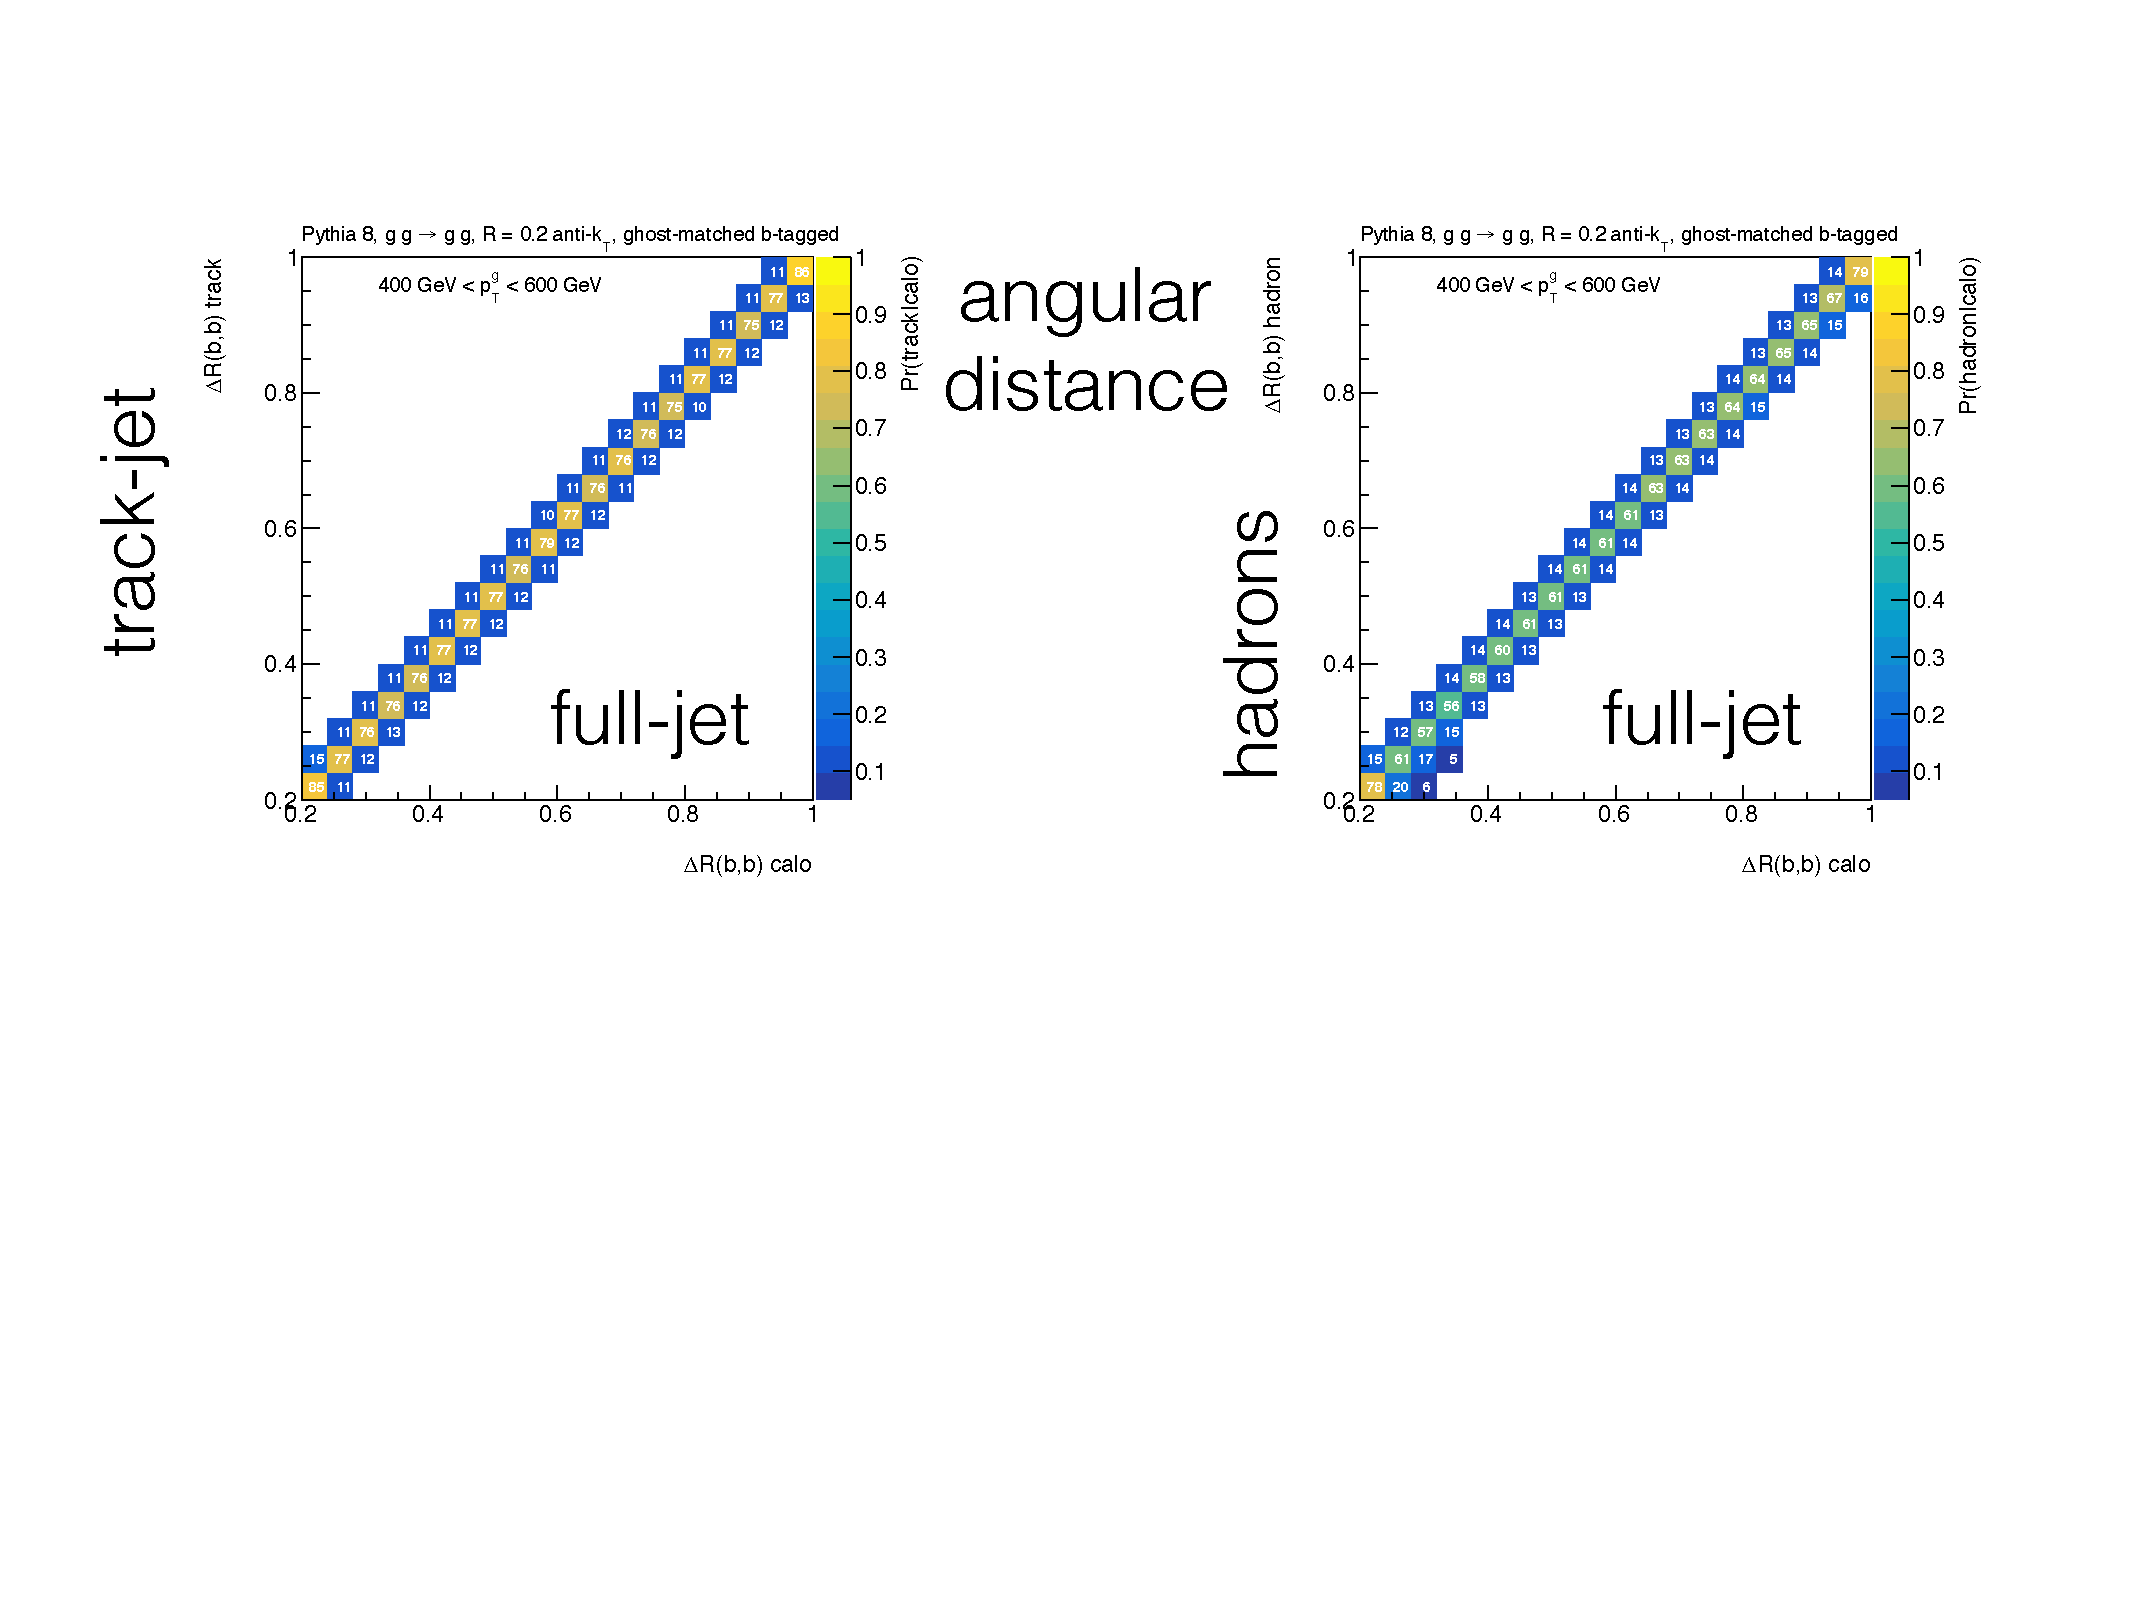
\includegraphics[width=0.95\linewidth]{figures/gbb/truth_level/compare2.pdf}\\
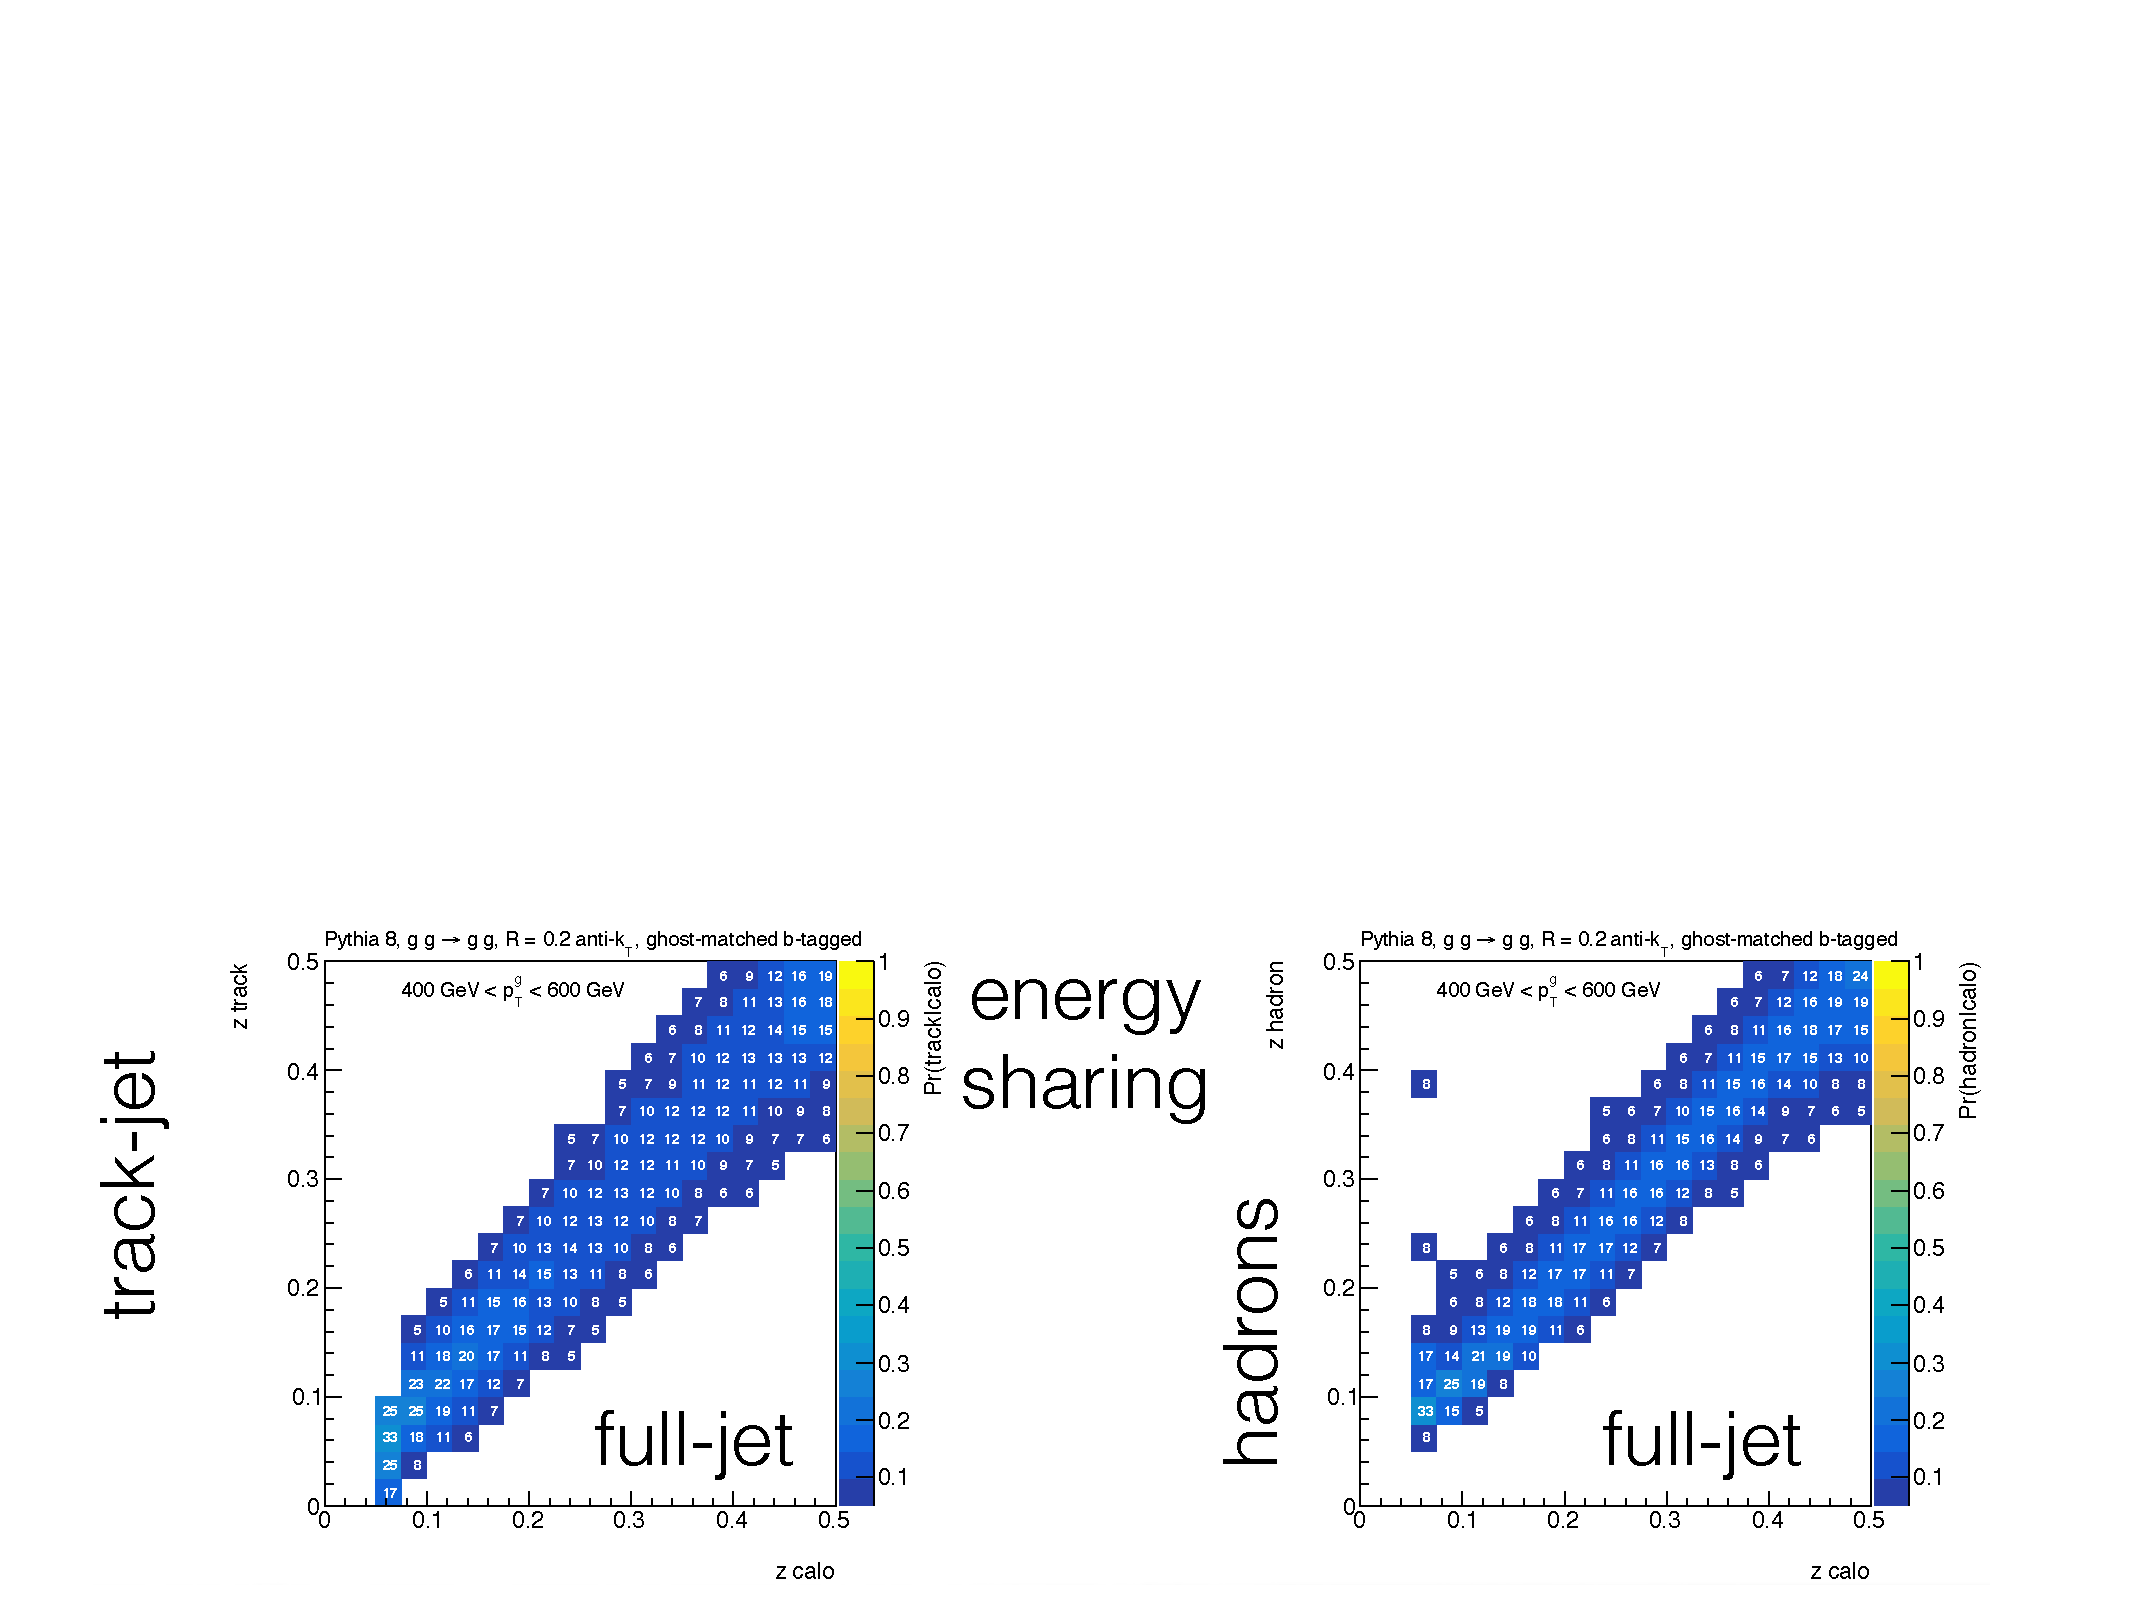
\includegraphics[width=0.95\linewidth]{figures/gbb/truth_level/compare1.pdf}
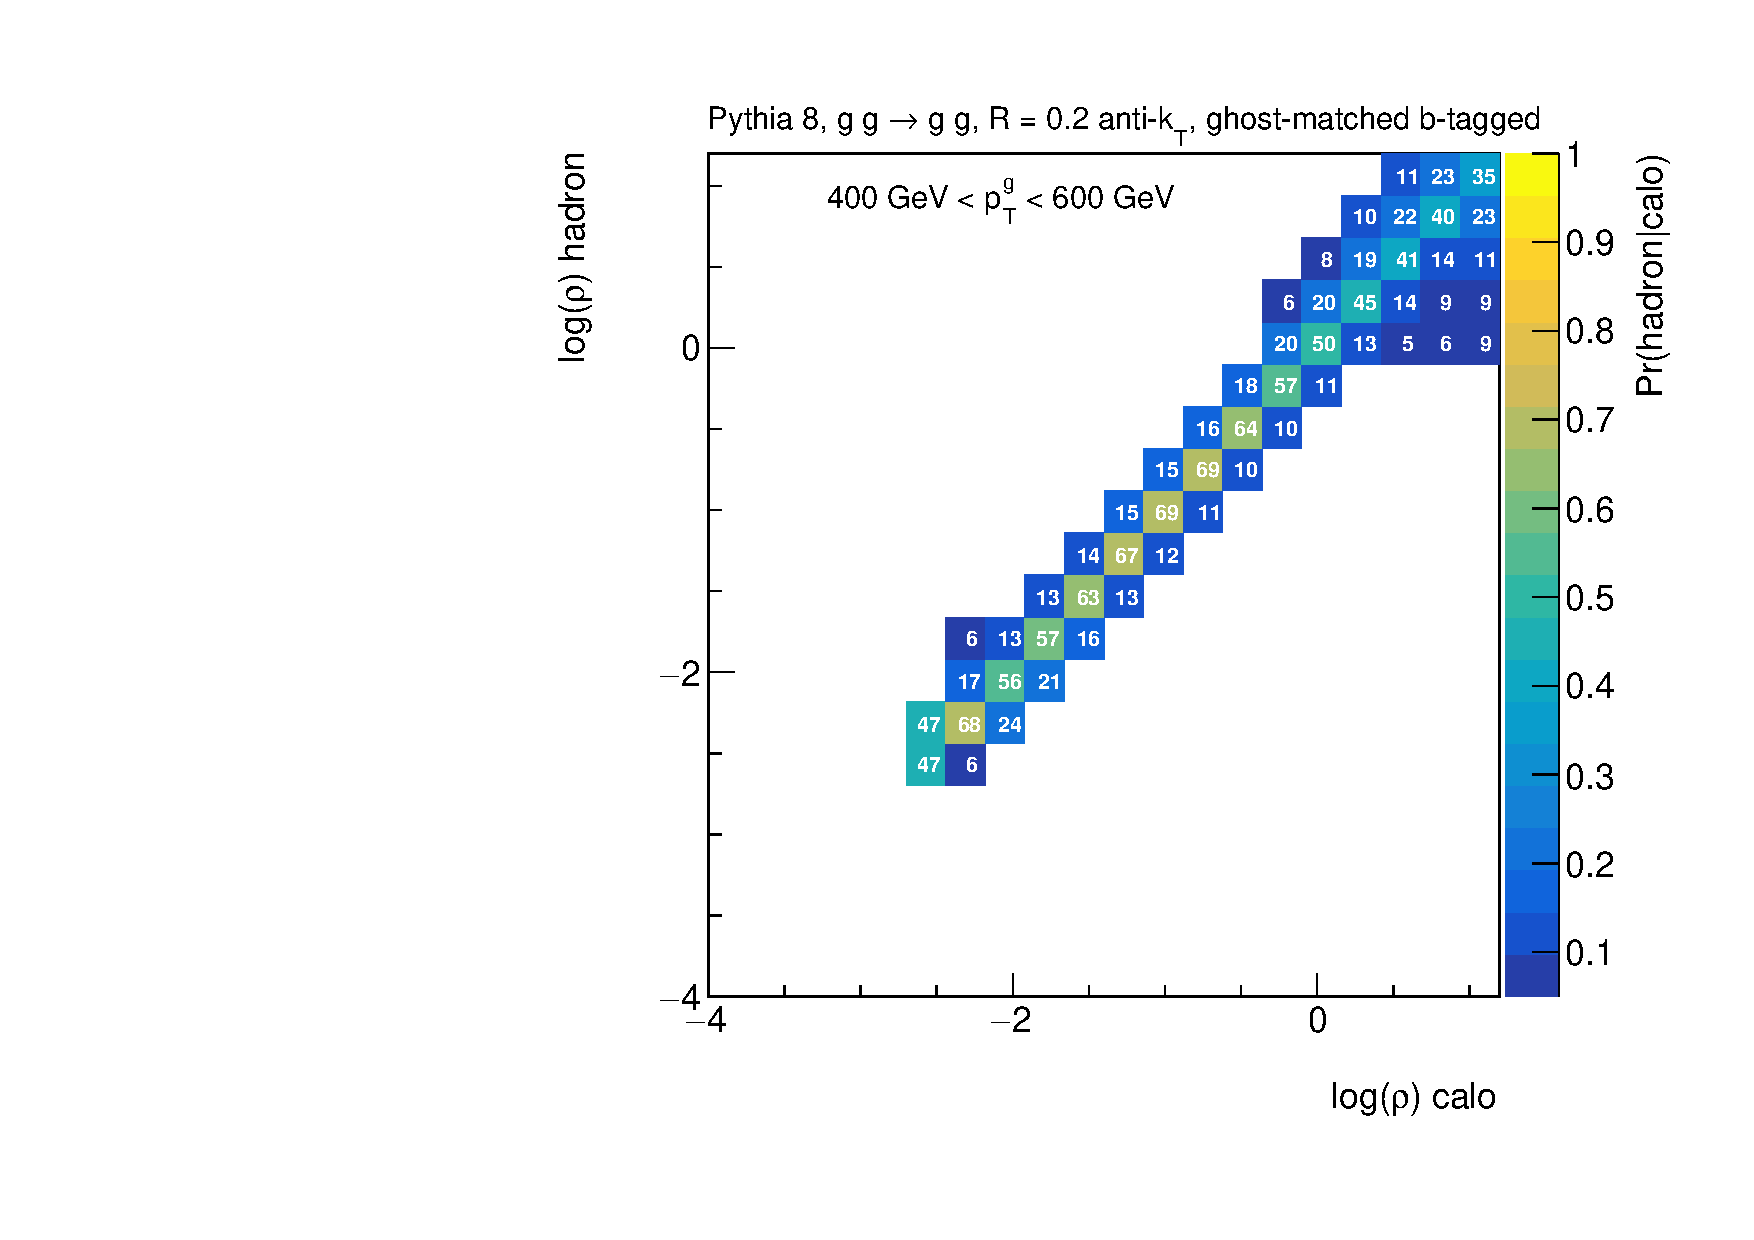
\includegraphics[width=0.45\linewidth]{figures/gbb/truth_level/rho_calo_track_b.pdf}
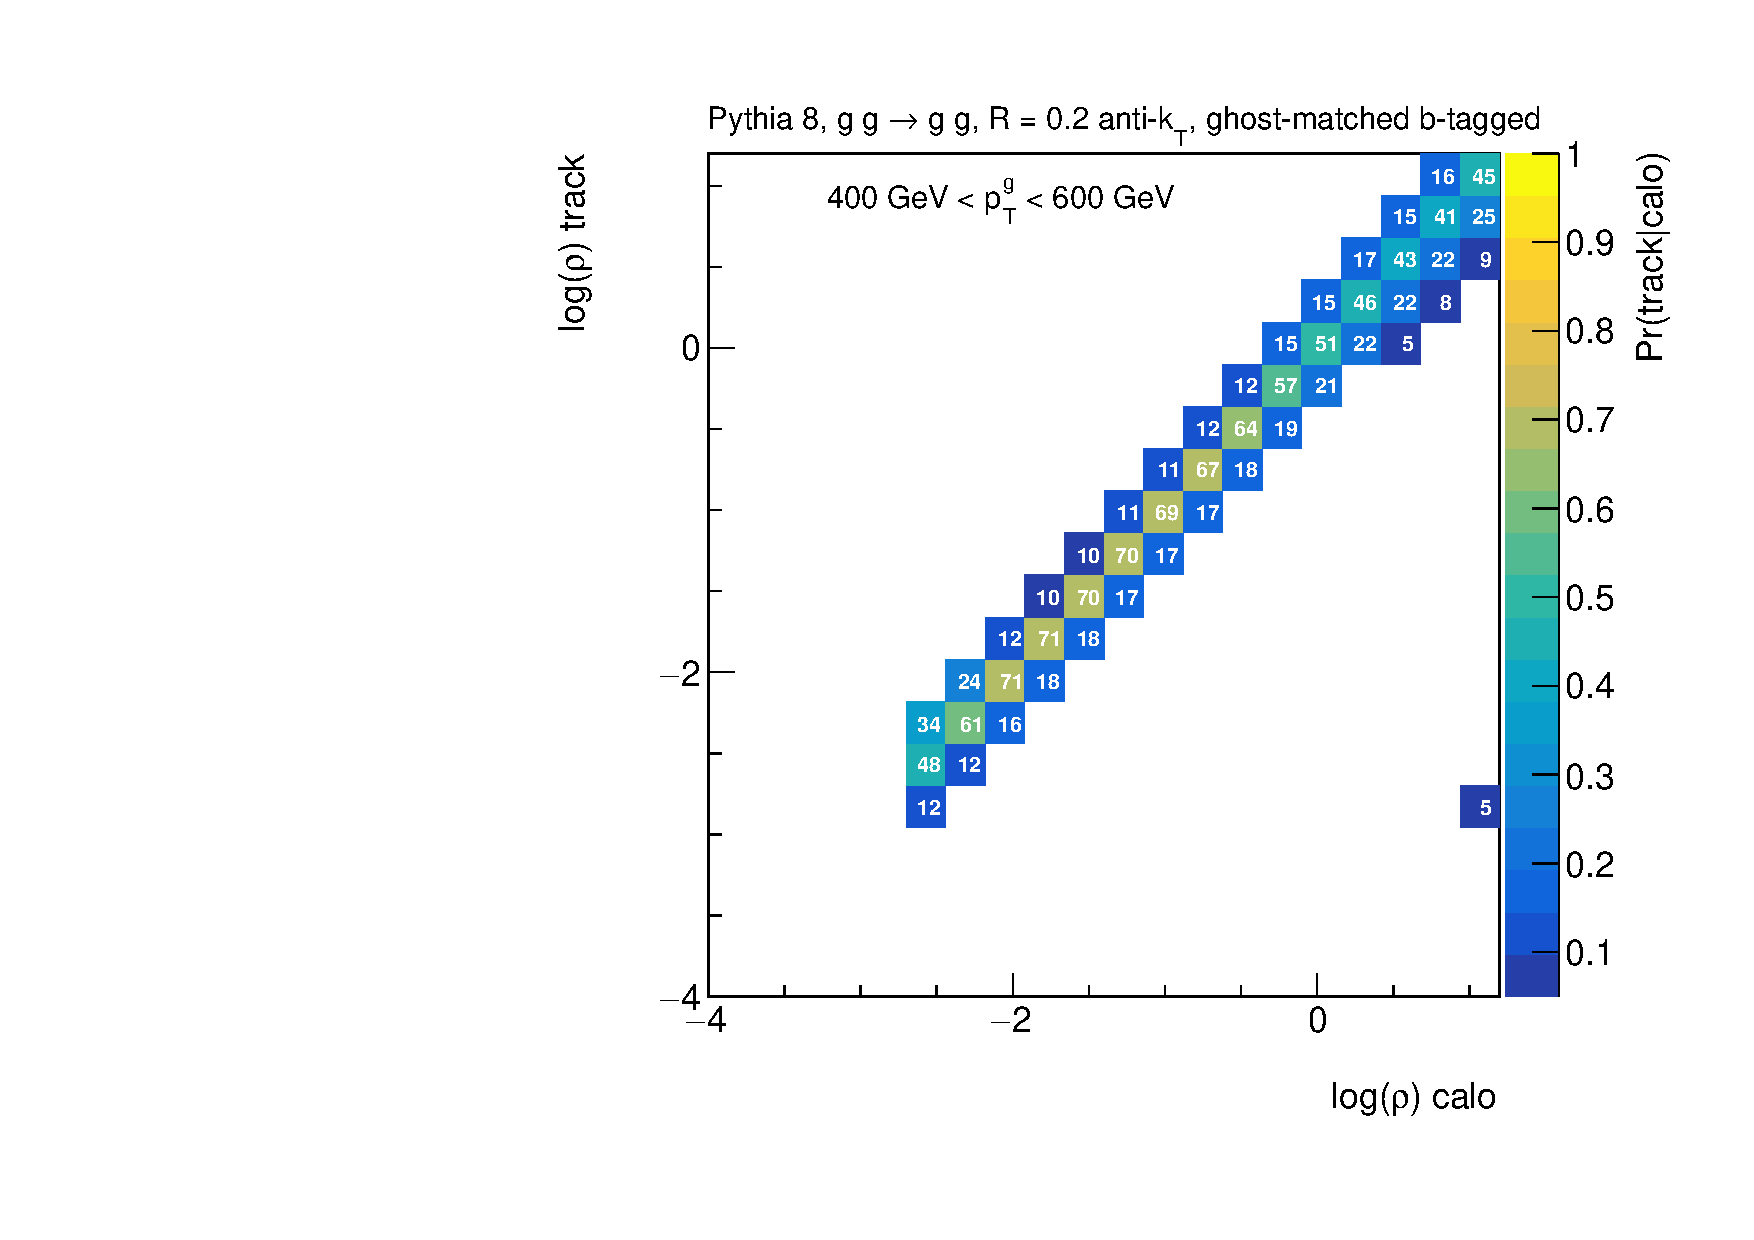
\includegraphics[width=0.45\linewidth]{figures/gbb/truth_level/rho_calo_track.pdf}
\caption{The two-dimensional distribution of two of the variables from Fig.~\ref{fig:gbb-gbbdistributions}, but using different definitions of `b' ($B$-hadrons, $b$-jets, $b$-track-jets).} 
\label{fig:gbb-gbbresponse}
\end{center}
\end{figure}

\begin{figure}[htpb!]
\begin{center}
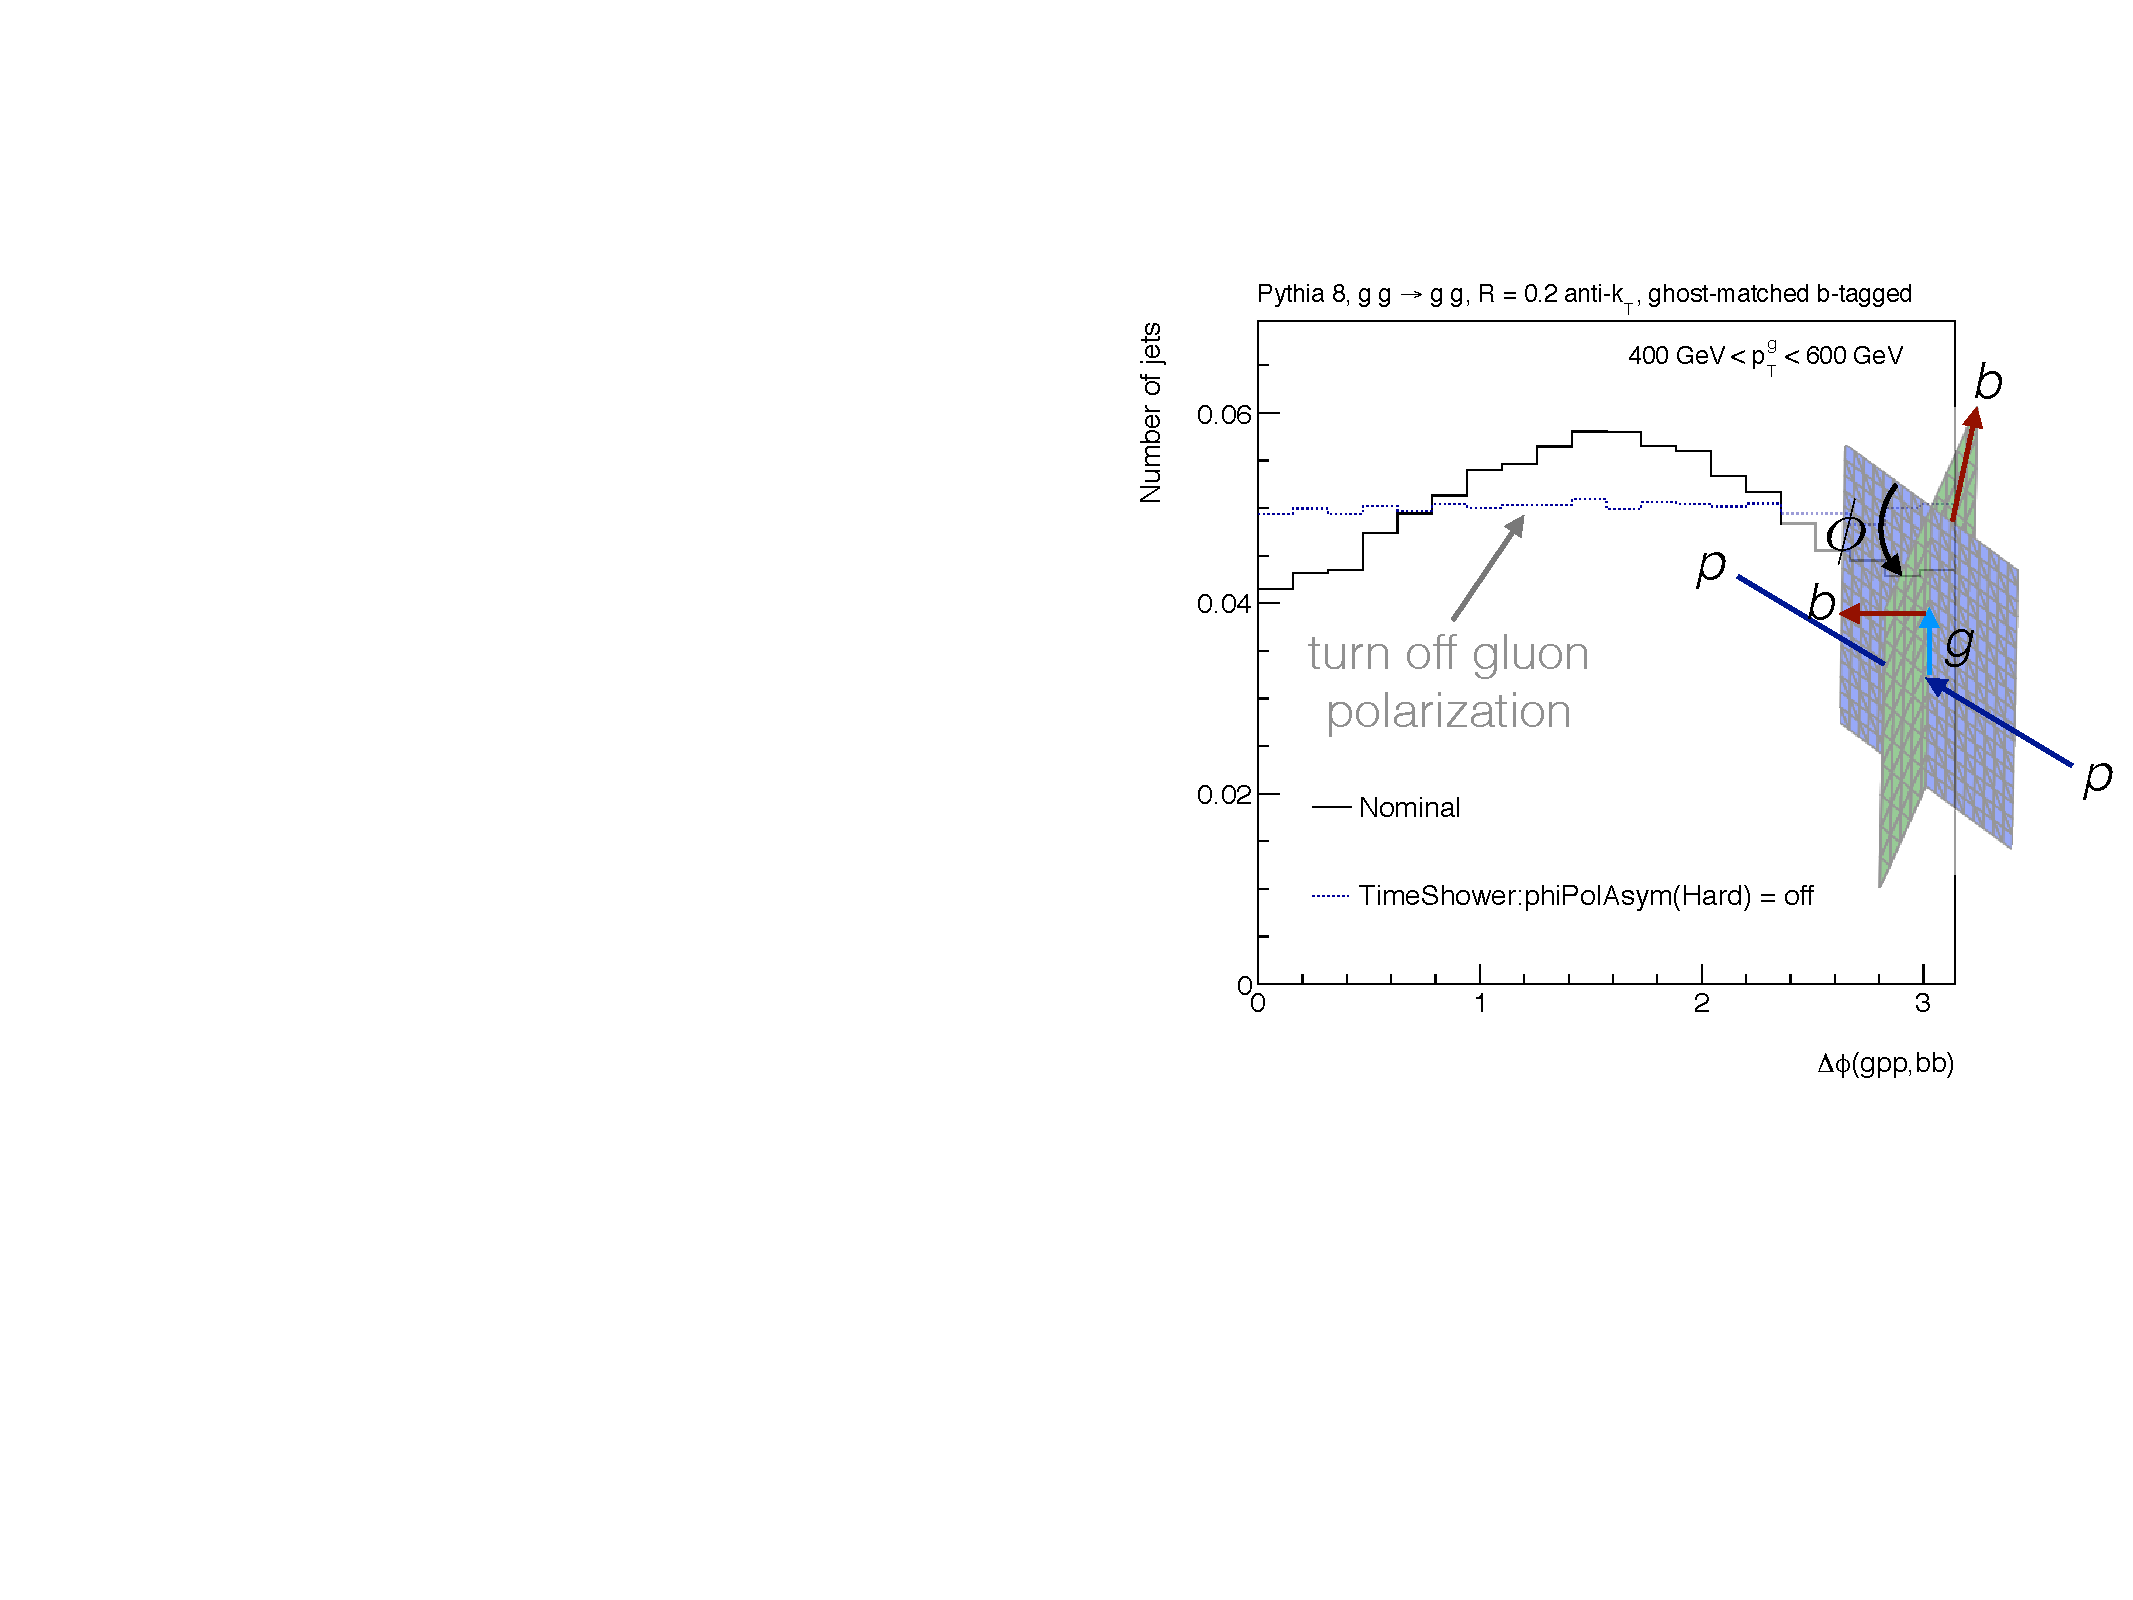
\includegraphics[width=0.45\linewidth]{figures/gbb/truth_level/phi.pdf}
\caption{The angle $\phi$ that the $g\rightarrow b\bar{b}$ plane makes with respect to the $pp\rightarrow g$ plane.  This distribution is sensitive to the gluon polarization.} 
\label{fig:gbb-gbbangle}
\end{center}
\end{figure}



\clearpage

%-------------------------------------------------------------------------------
\section{Background Estimation}
\label{sec:backgrounds}
%-------------------------------------------------------------------------------
\label{sec:gbb-bkgsub}
\subsection{Flavor Fractions}
Post \btagging, a large fraction of events are backgrounds as shown in Table~\ref{tab:posttaggingflav}. To unfold the data, subtraction of the remnant background is necessary. It is a known problem that the nominal MC flavor fractions could deviate from the true values in data (see e.g.~\cite{ATLAS-CONF-2016-002}). To have good control over the flavor fractions, we seek to estimate the flavor fractions in bins of each observable by fitting the distributions of some variables, which may not be powerful enough to tag individual jets, but are sensitive to the numbers of jets of different flavors. 

\begin{table}[htbp]
\centering
\resizebox{\textwidth}{!}{
\begin{tabular}{|l|l|l|l|l|l|l|l|l|l|}
\hline
Flavor Combination & BB      & BC     & BL     & CB     & CC     & CL     & LB     & LC     & LL     \\ \hline
Flavor Fraction    & 19.01\% & 2.20\% & 34.68\% & 0.39\% & 5.73\% & 17.99\% & 0.37\% & 0.86\% & 18.76\% \\ \hline
\end{tabular}}
\caption{Post $b$-tagging flavor composition in MC. The first letter of the flavor combination is the flavor of the leading jet. The second letter of the combination is the flavor of the sub-leading jet. }
\label{tab:posttaggingflav}
\end{table}


\subsection{$s_{d_{0}}$ as Discriminant Variable }
\label{sec:gbb-sd0}

The long decay length of heavy flavor hadrons make the signed significance of impact parameter $s_{d_{0}}$ of tracks associated to a jet a good discriminating variable. The $s_{d_{0}}$ is defined as 
\begin{equation}
s_{d_{0}} = \frac{d_0}{\sigma(d_0)} \cdot s_{j}
\end{equation}
where $d_{0}$ is the track transverse impact parameter, $\sigma(d_{0})$ is the uncertainty on the $d_0$ measurement, and $s_{j}$ is the sign of $d_{0}$ with respect to the jet axis. The variable $s_j$ is defined as
\begin{equation}
s_{j} = \textrm{sign}\left\{\ \sin\left(\arctan \left( \frac{p_{j,\ y}}{p_{j,\ x}}\right) - \phi_t\right) \cdot d_{0} \ \right\}
\end{equation}
 where $p_{j,\ x}$ and $p_{j,\ y}$ are the $x$ and $y$ components of the jet moments, respectively, and $\phi_{t}$ is the azimuthal angle of the track.
 
For a given track jet, by construction we have at least two tracks as constituents of the jet. %(number of track constituents distributions are shown in Fig.\ref{fig:gbb-ntrk}).
We take the sub-leading $s_{d_{0}}$ of the track (leading means highest value of $|s_{d_{0}}|$, sub-leading is second largest, etc.) as \subsdzero and build templates of different flavors using this variable to fit and derive the flavor fractions from data.   The second highest $s_{d_{0}}$ is used because it is less likely the result of mis-measured track parameters for non-$b$-jets. For illustration of the impact parameter significance please refer back to Fig.\ref{fig:reco-trkdef}.


%\begin{figure}[htbp]
%  \centering
% 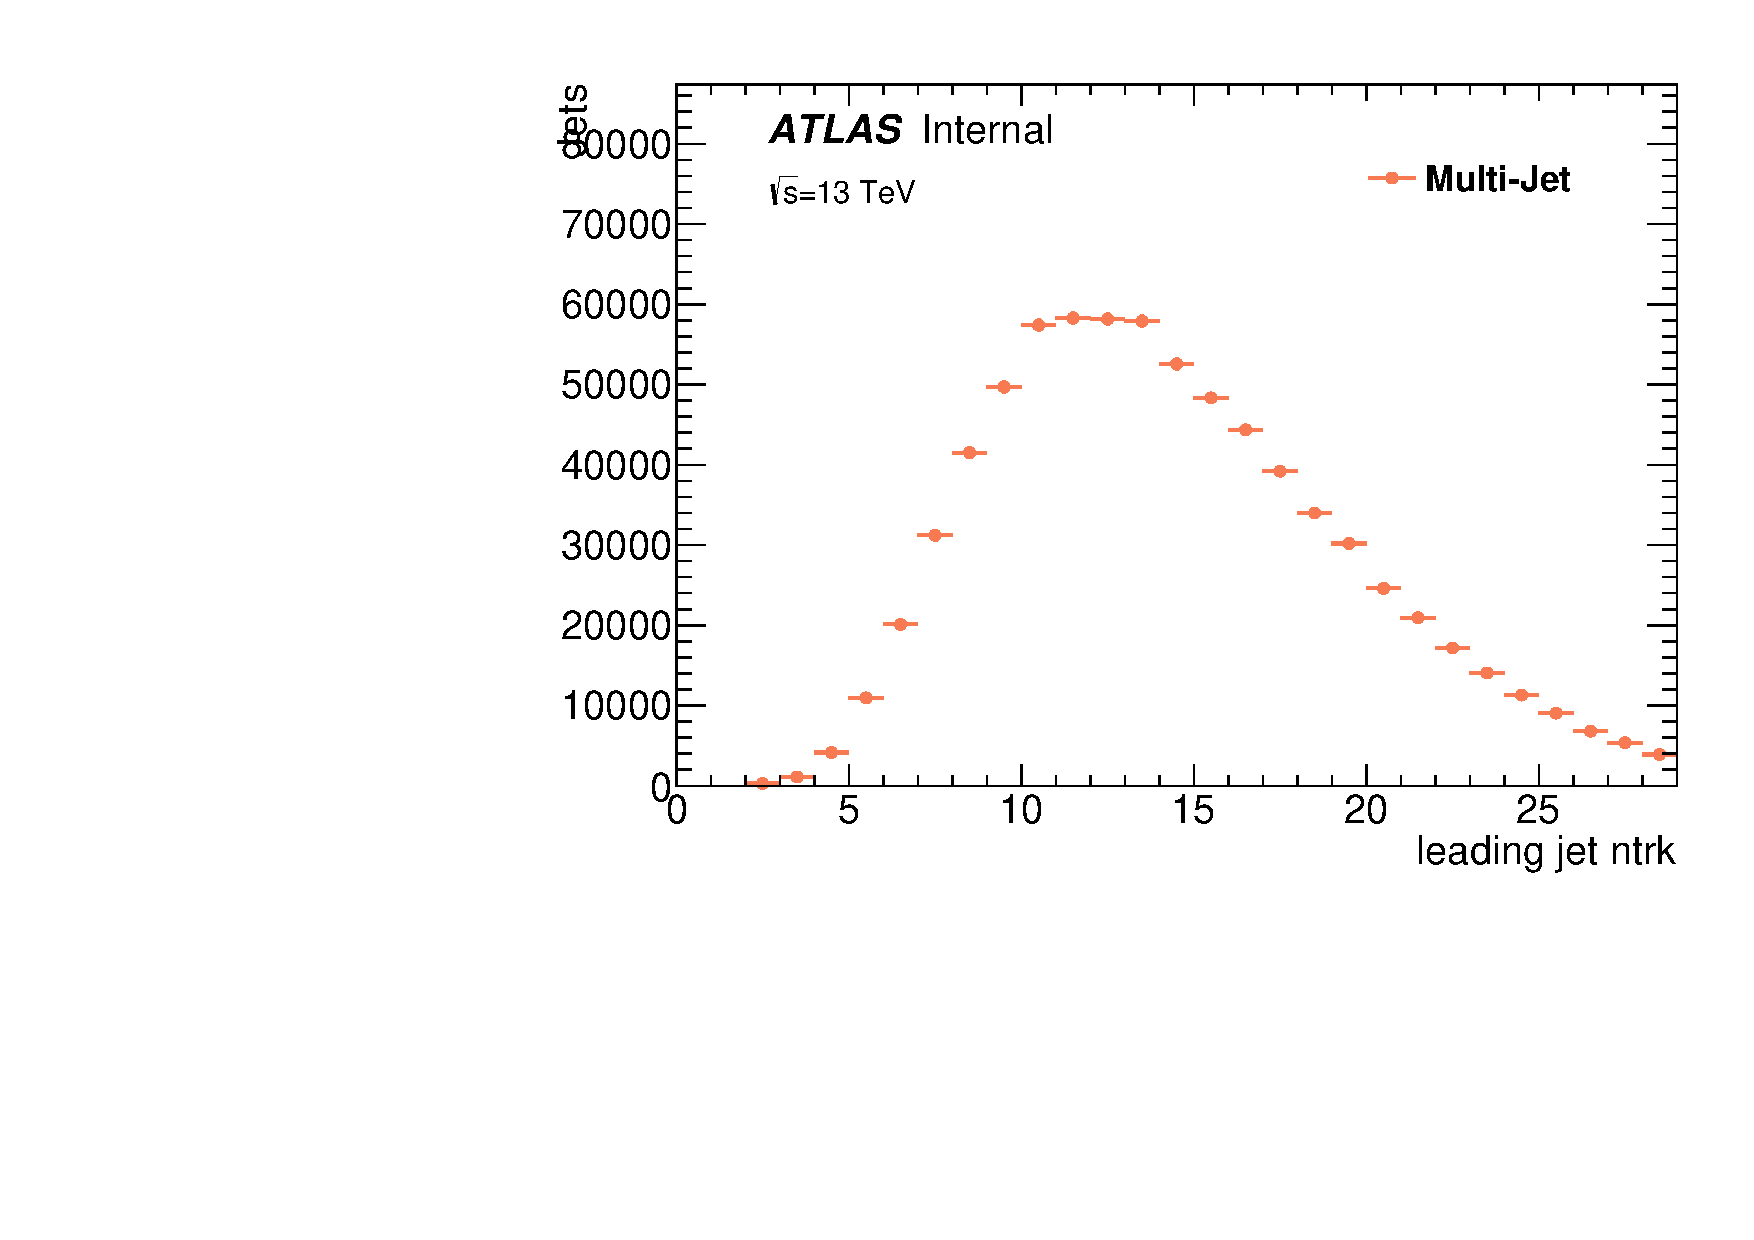
\includegraphics[width=0.48\textwidth]{figures/gbb/Leading_trkjet_ntrk_PostTag.pdf}
% 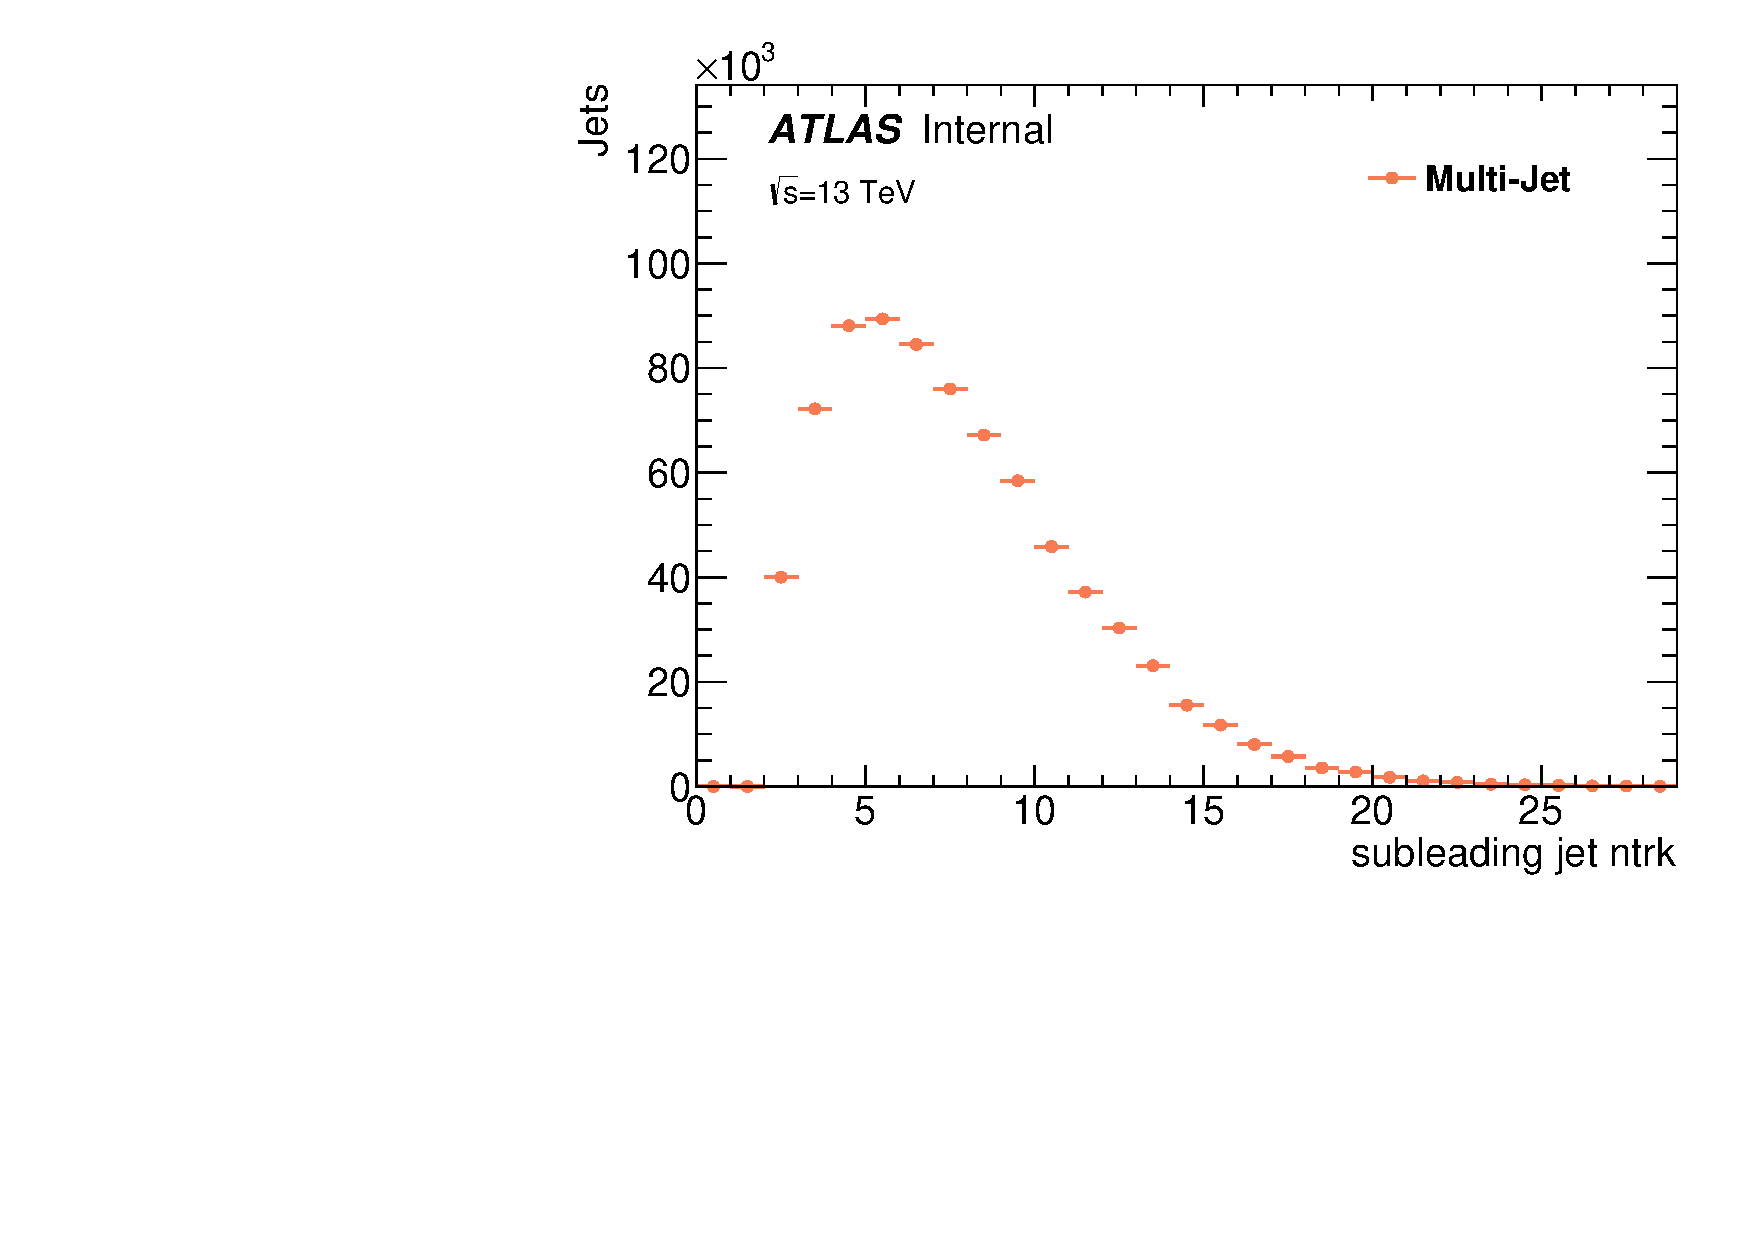
\includegraphics[width=0.48\textwidth]{figures/gbb/SubLeading_trkjet_ntrk_PostTag.pdf}\\
%\caption{The number of track distribution for leading (left) and sub-leading (right) track jets in MC prediction}
%  \label{fig:gbb-ntrk}
%\end{figure}


%%%%%%%%%%%%%%%%%%%%%%%%%%%%%%%%%%%%%%%%%%%%%%%%%

\subsection{Binned Maximum Likelihood Estimation}

An $m$ flavor component template fit ($m = 3$ for the fit we perform) is carried out by maximizing a binned likelihood function defined as $\mathcal{L} = \prod _{i=1} ^n p(y_i| \vec{\theta})$, where $\vec{\theta} \in \mathbb{R}^m$ denotes the number of events from each flavor component, $n$ is the number of bins we are fitting and $y_i$ is the number of data events in bin $i$. The assumption of $p(y_i|\vec{\theta})$ is Poisson distribution: 
\begin{equation}
p(y_i|\vec{\theta}) = \frac{\exp{(-\vec{\theta} \vec{\cdot x_i)}} {(\vec{\theta}} \vec{\cdot x_i})^{y_i}}{y_i !}, 
\end{equation}
where $\vec{x_i}=(x_{i1}...,x_{ij}...,x_{im}) \in \mathbb{R}^m$ is a vector, and each component denotes the $i^{th}$ bin value in the normalized templates for the $j^{th}$ flavor ($b$, $c$ and light).   We determine the flavor fractions by finding the $\vec{\theta}$ that maximizes $\mathcal{L}$. The fit is carried out by the MIGRAD function of the MINUIT package. 

%%%%%%%%%%%%%%%%%%%%%%%%%%%%%%%
\subsection{\subsdzero Templates }
\label{sec:gbb-subdzerotemplates}

The flavor contents of the two $R=0.2$ jets in a $R=1.0$ jet are correlated. 
Tagging one of the $b$ jets increases the probability of the other track jet 
being a $b$ jet. Therefore, we should not treat the flavor 
contents of the two jets independently and thus must take into account both jets 
flavors simultaneously when fitting. On the other hand, given the flavors of the 
two $R= 0.2$ jets, their \subsdzero values are not correlated, as shown in Table \ref{tab:sd0cor}. 
Therefore, we can derive the flavor fractions by fitting simultaneously the 
1-dimensional \subsdzero distributions of the leading and sub-leading jets
 using templates derived from all of the possible 2-jet flavor pair 
combinations. This is essentially a Naive Bayes approximation, i.e. assuming the joint 
2-D probability density is the product of the two 1-D probability density
 $p(\subsdzero(j1), \subsdzero(j2)) = p(\subsdzero(j1))p(\subsdzero(j2))$.

\begin{table}[htbp]
\centering
\begin{tabular}{|r|r|r|r|}
\hline
\centering
Flavor Combination & \subsdzero Correlation Factor\\
\hline
BB & 0.7\% \\
BL & 0.4\% \\
BC & -2.2\% \\
LB & 3.9\%\\
LL & 0.3\%\\
LC & 0.8\%\\
CB & -0.3\% \\
CL & 0.5\% \\
CC & -4.1\% \\

\hline
\end{tabular}%
\caption{Correlation factor between the \subsdzero values of the two R = 0.2 jets.}
\label{tab:sd0cor}
\end{table}%

There are in total nine different ordered flavor pairs: BB, BL, BC, CB, CL, CC, 
LB, LC and LL such that the first flavor is that of the leading track jet and 
the second is that of the other track jet. Many of these components are very small 
for us to fit their contributions correctly as show in Table~\ref{tab:posttaggingflav}. 
Therefore, starting with BL, CL templates, we merge other templates to these templates
to form B-like and C/L-like templates. The metric we use for determining the similarity 
between two distributions is: $S=\frac{1}{2}\int \frac{(p_1(x)-p_2(x))^2}{p_1(x)+p_2(x)}$, 
where $p_1(x)$ and $p_2(x)$ are two different distributions. 
Based on calculation, we merge the BC template with the BL 
template, and other components into CL as seen in 
Table \ref{tab:overlap-unmerged}. The merged templates are 
presented in Figure \ref{fig:gbb-templates} and the separation powers estimated by the same metric are 
presented in Table \ref{tab:overlap-merged}. 
We show the full set of templates in bins of the observables we are interested in 
measuring in Appendix~\ref{sec:gbb-app-sd0templates}. 

It is noteworthy that the statistics of our Monte Carlo samples is low.
Presumably, a double $b$-tagging strategy would be preferable as it could filter 
out most of the background processes.
However, double $b$-tagging strategy would also yield background templates with large 
statistical fluctuations. In Fig. \ref{fig:gbb-template-leadtight-medium} the comparison 
of the templates derived from single $b$-tagging and double $b$-tagging (at 70\% $b$-
efficiency for both jets) in one bin of $\Delta R$ is shown. The considerable statistical uncertainties ($\geq 10\%$ relative uncertainty per bin in template)
of double $b$-tagging strategy lead us to use single $b$-tagging strategy instead. 


\begin{table}[htpb]
\centering
\begin{tabular}{|l|l|l|l|l|}
\hline
   & BL   & CL    & BB   \\ \hline
BC & 0.02 & 0.08  & 0.11 \\ \hline
CC & 0.09 & 0.03  & 0.14 \\ \hline
LC & 0.07 & 0.05  & 0.12 \\ \hline
LB & 0.17 & 0.12  & 0.05 \\ \hline
CB & 0.19 & 0.14  & 0.08 \\ \hline
LL & 0.02 & 0.01  & 0.17 \\ \hline
BB & 0.16 & 0.21  & 0    \\ \hline

\end{tabular}
\caption{Templates similarity calculated using the metric $S=\frac{1}{2}\int \frac{(p_1(x)-p_2(x))^2}{p_1(x)+p_2(x)}$ for un-merged templates. Given two distributions $p_1(x)$ and $p_2(x)$, the metric returns 0 if they are exactly the same and returns 1 if there is no overlap between them.}
\label{tab:overlap-unmerged}
\end{table}



\begin{table}[htpb]
\centering
\begin{tabular}{|l|l|l|l|l|}
\hline
    & B    & L+C    & BB   \\ \hline
B   & 0    & 0.04  & 0.16 \\ \hline
L+C & 0.04 & 0     & 0.17 \\ \hline
BB  & 0.16 & 0.17  & 0    \\ \hline

\end{tabular}
\caption{Templates similarity calculated using the metric $S=\frac{1}{2}\int \frac{(p_1(x)-p_2(x))^2}{p_1(x)+p_2(x)}$ for merged templates. Given two distributions $p_1(x)$ and $p_2(x)$, the metric returns 0 if they are exactly the same and returns 1 if there is no overlap between them.}
\label{tab:overlap-merged}
\end{table}


\begin{figure}[htbp]
  \centering
 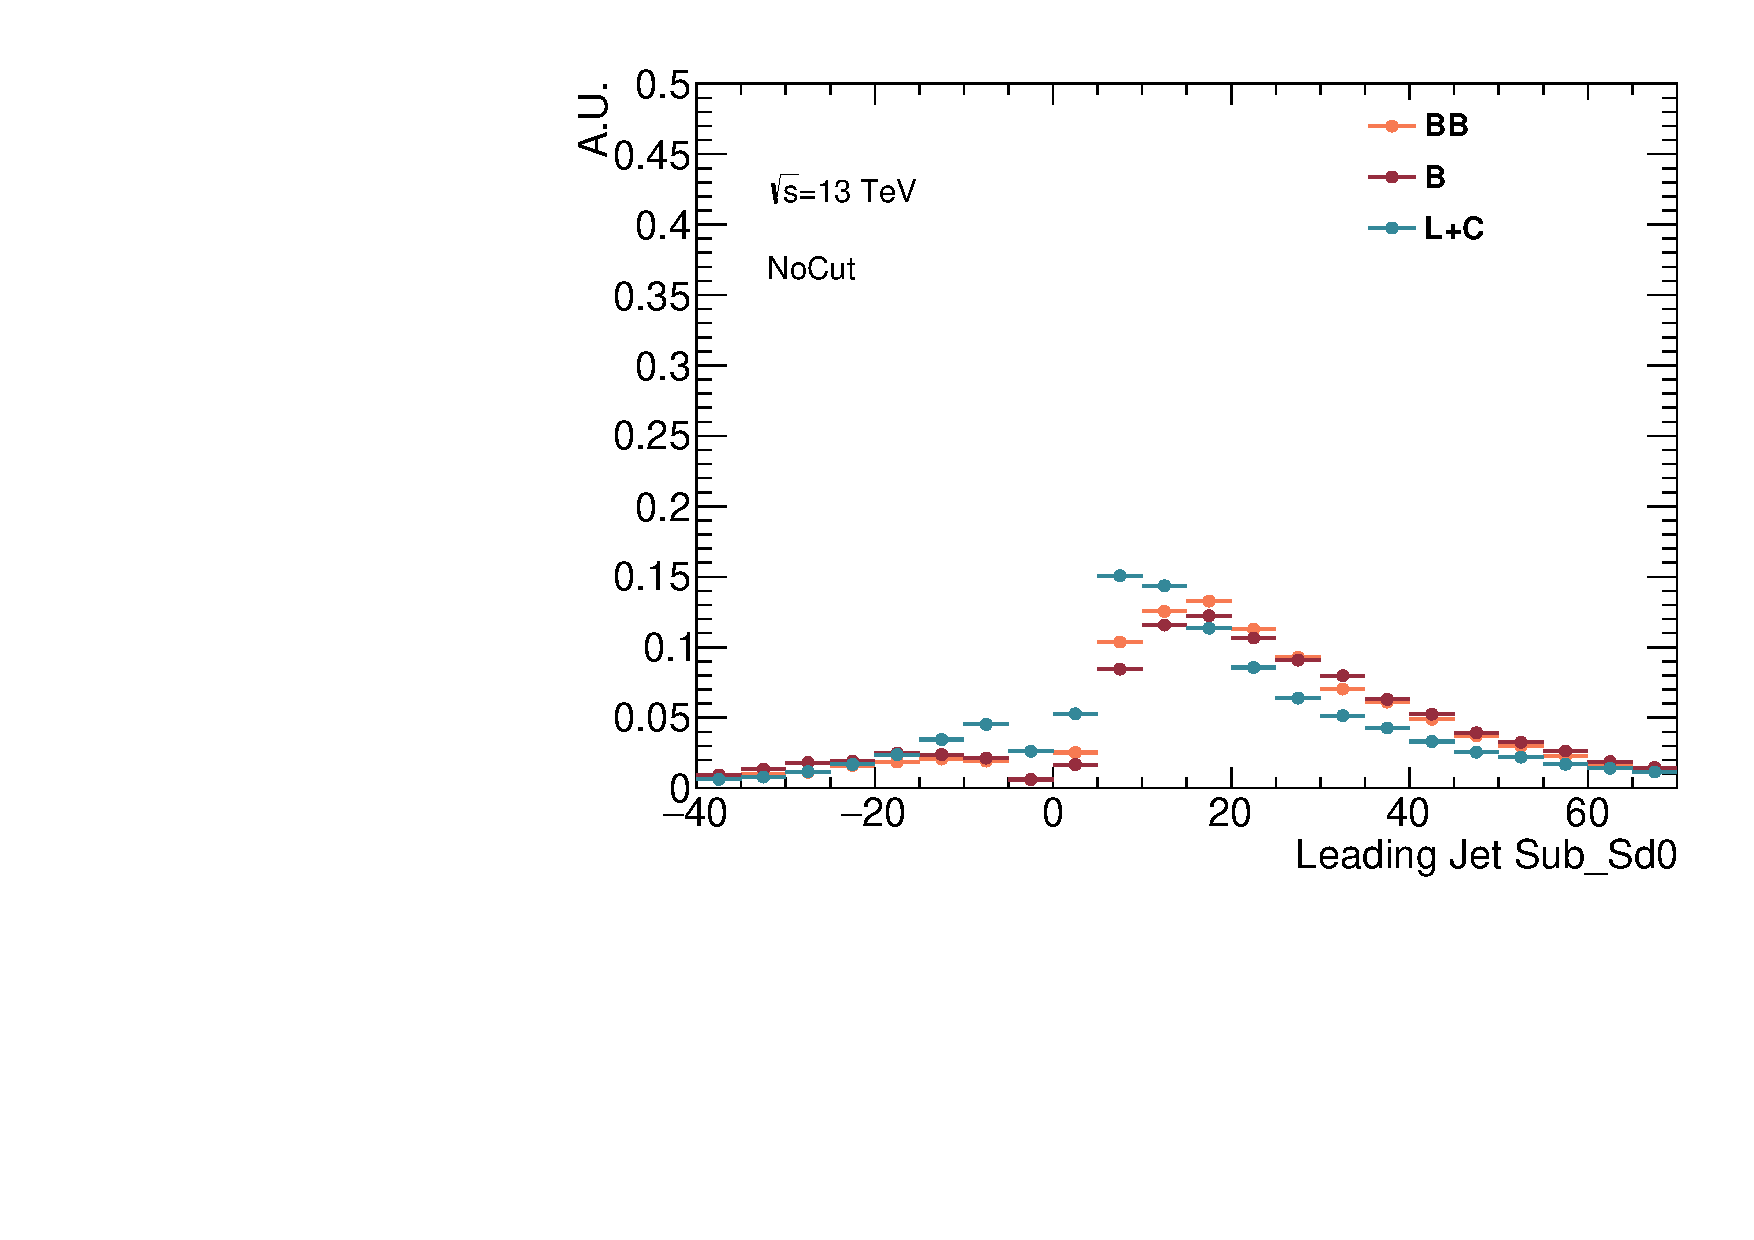
\includegraphics[width=0.48\textwidth]{figures/gbb/Sub_Sd0_Fits/Canv_FitTemplate_Inclusive_x.pdf}
 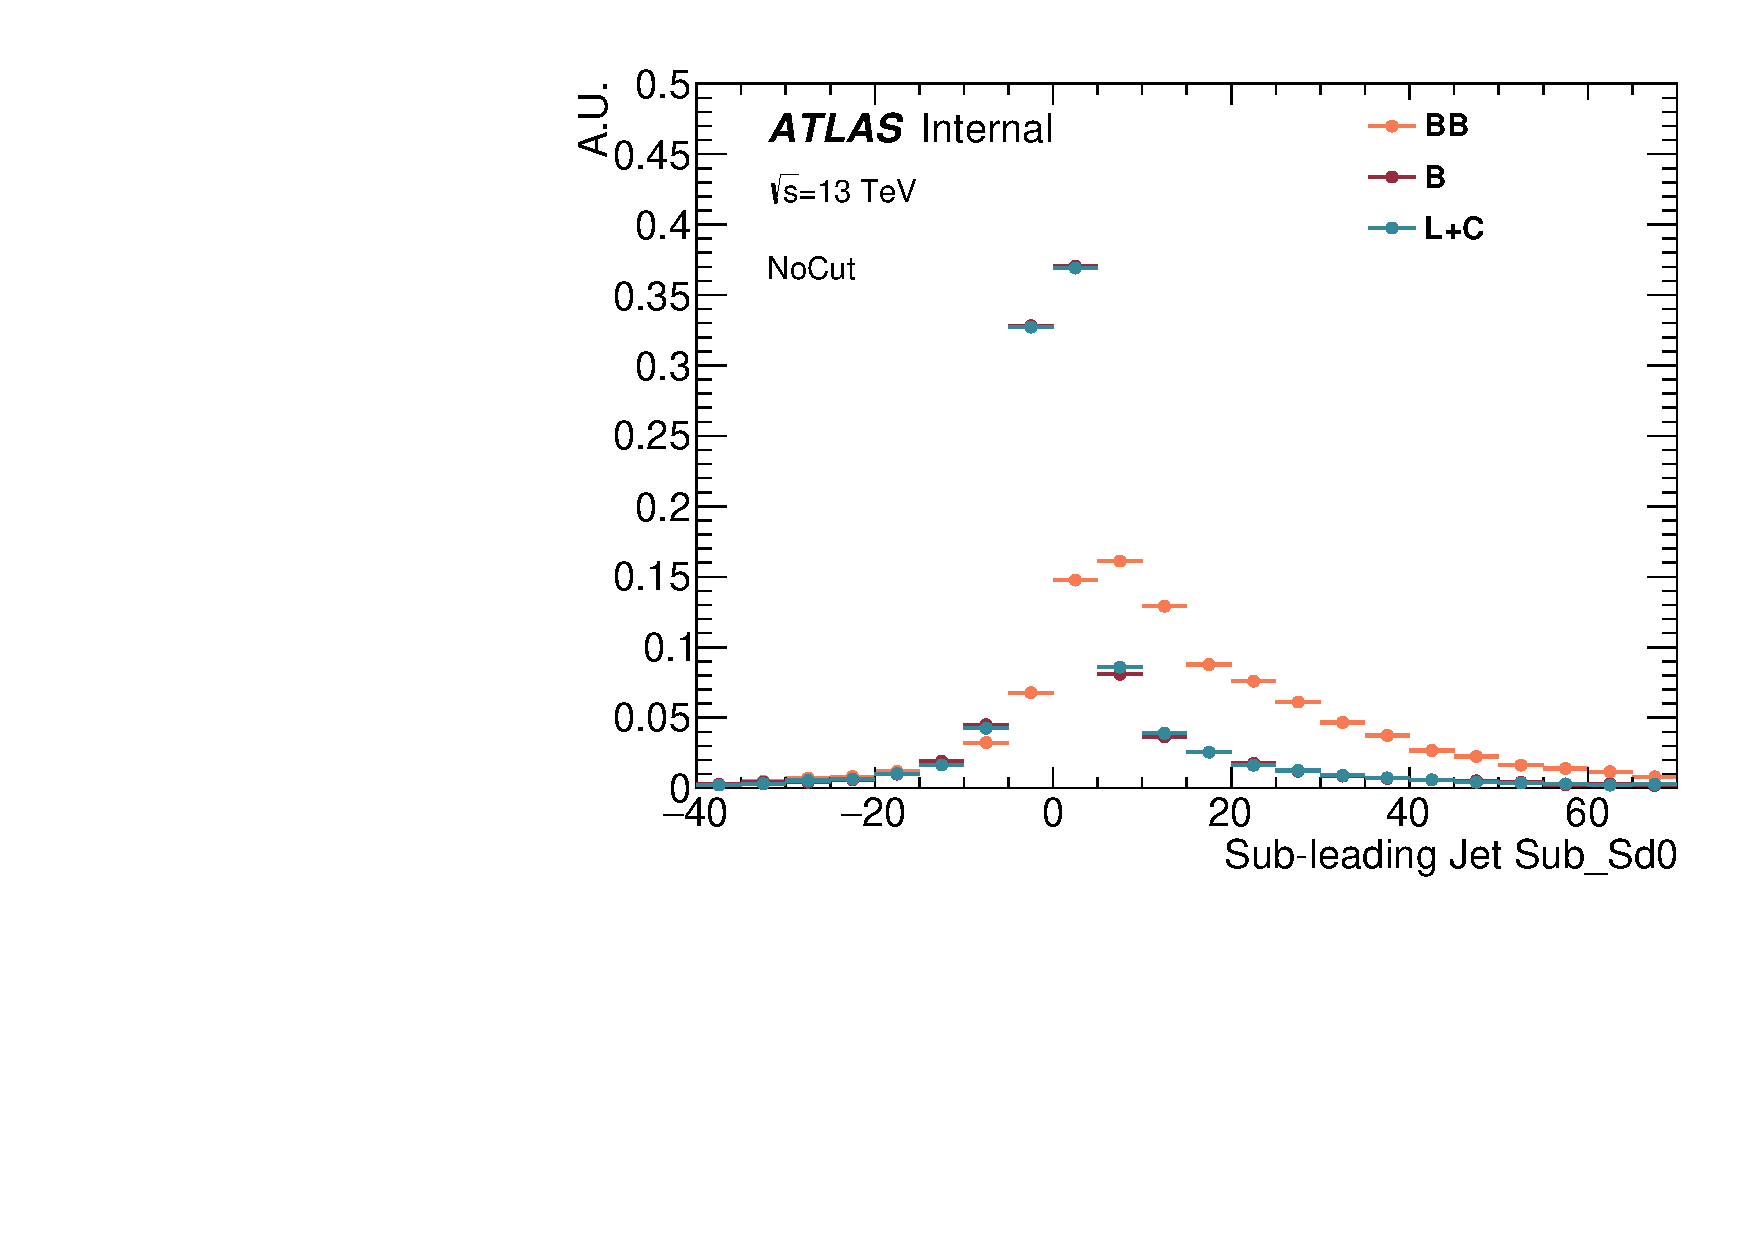
\includegraphics[width=0.48\textwidth]{figures/gbb/Sub_Sd0_Fits/Canv_FitTemplate_Inclusive_y.pdf}\\
\caption{The merged \subsdzero templates (inclusive) for leading (left) and sub-leading (right) track jets.}
  \label{fig:gbb-templates}
\end{figure}


\begin{figure}[htbp]
  \centering
 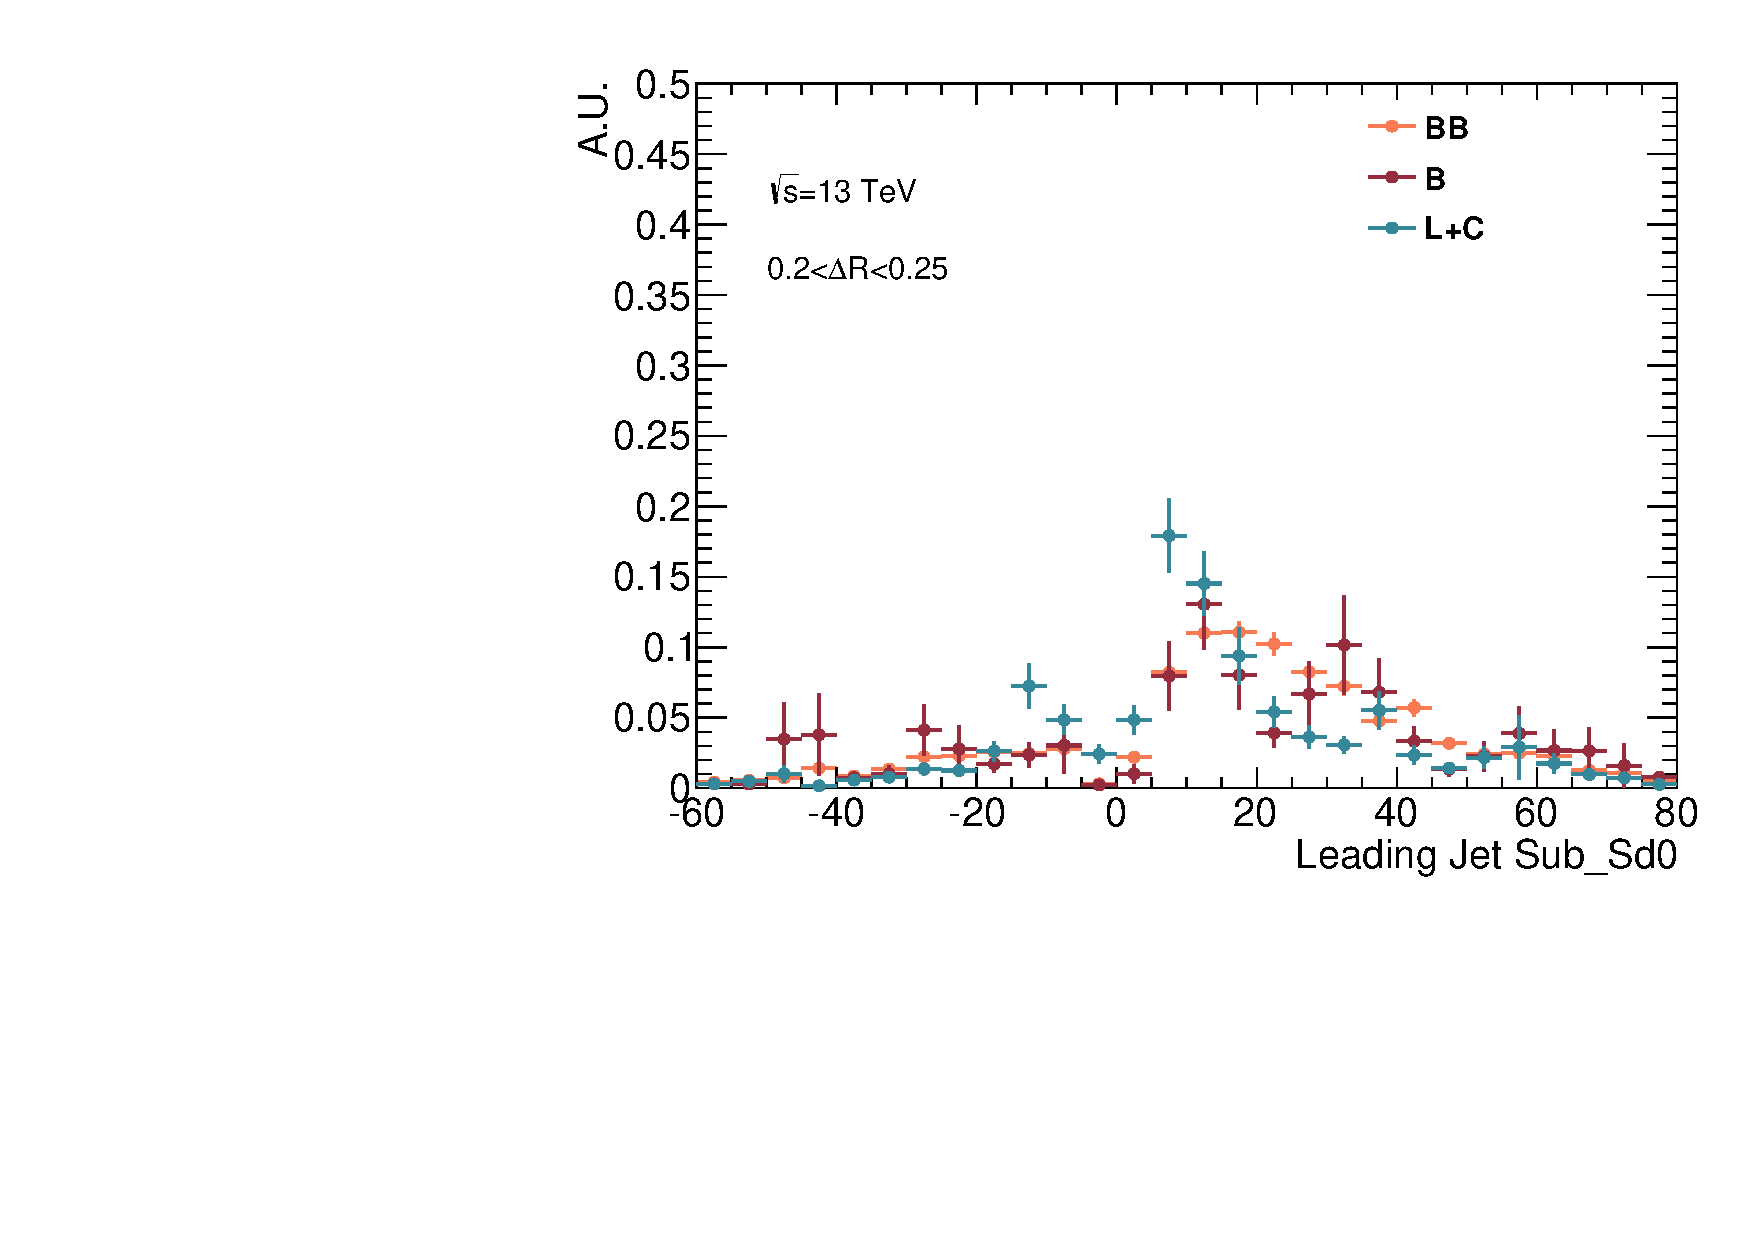
\includegraphics[width=0.48\textwidth]{figures/gbb/Canv_FitTemplate_medium.pdf}
 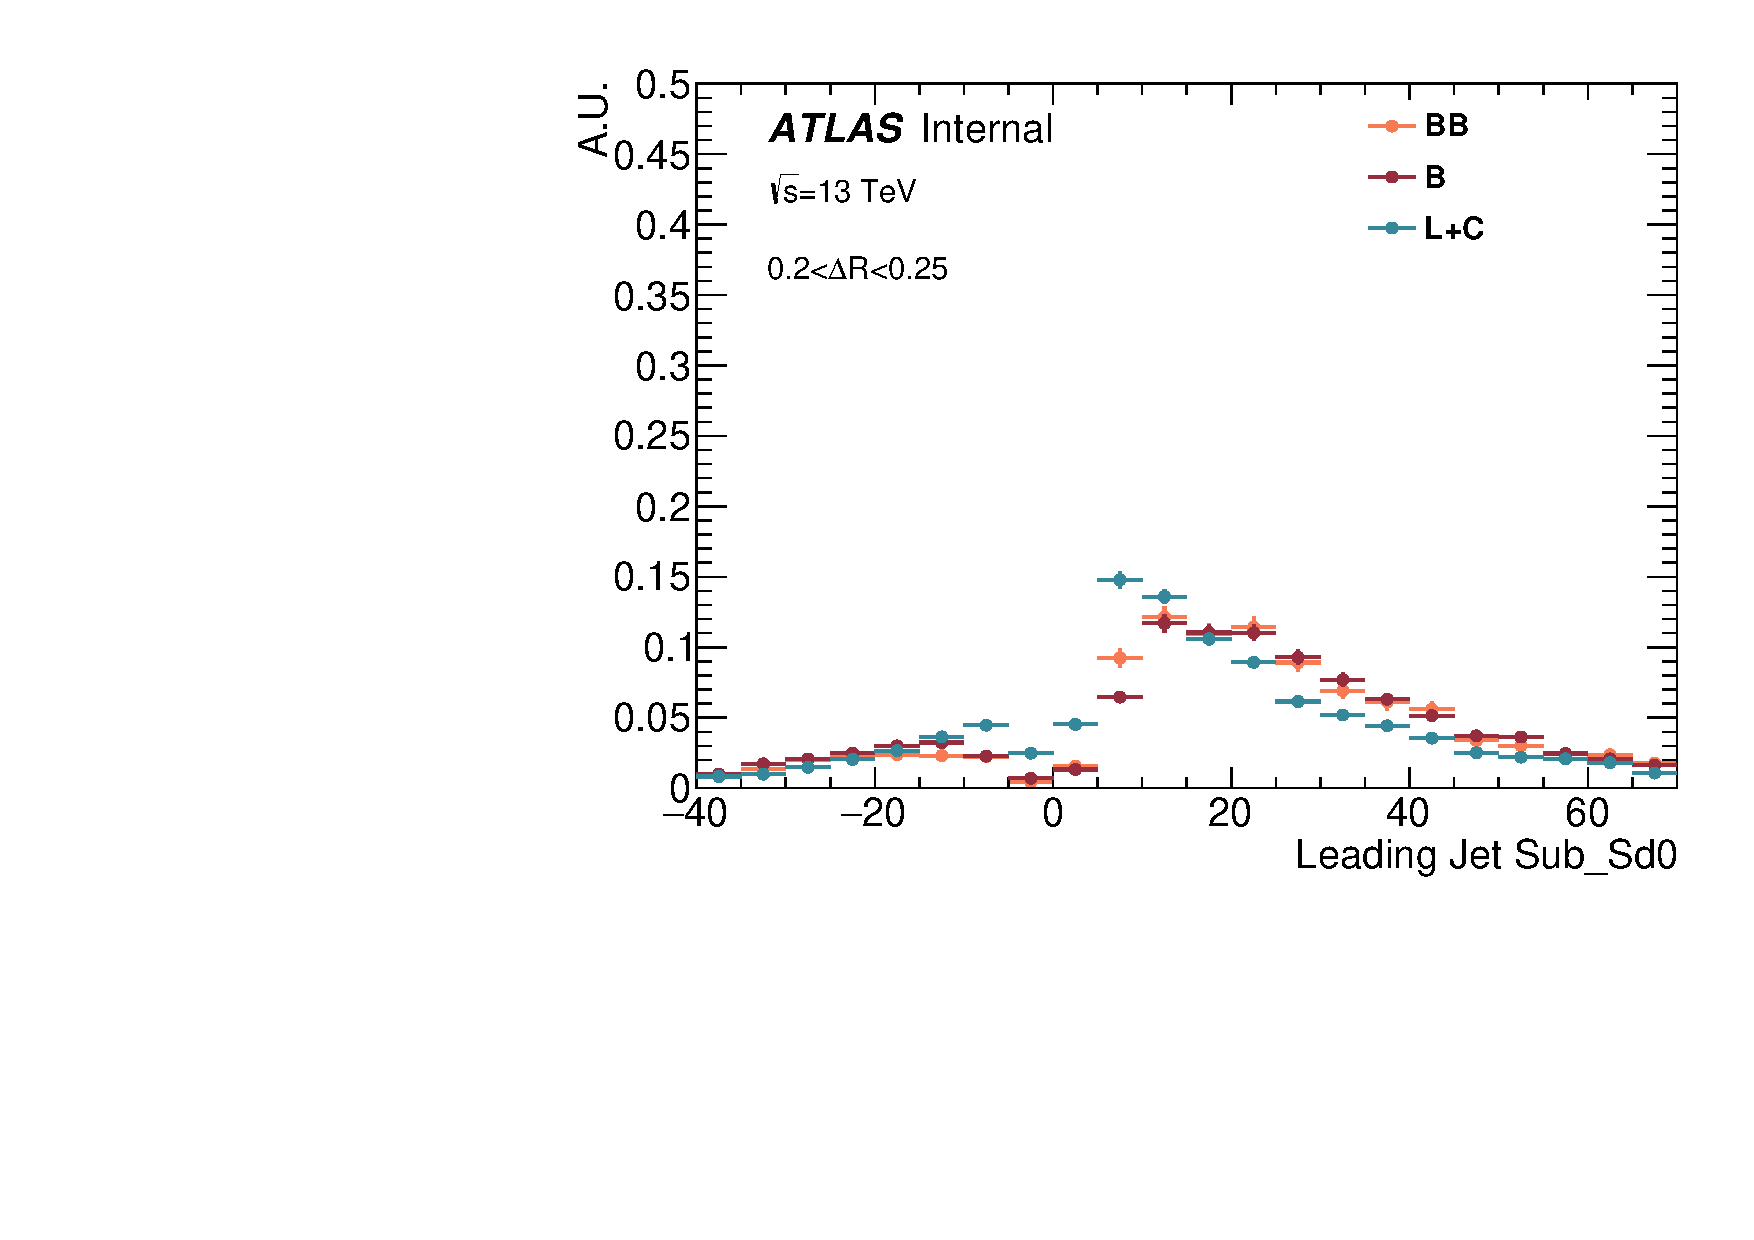
\includegraphics[width=0.48\textwidth]{figures/gbb/Sub_Sd0_Fits/Canv_FitTemplate_02-DeltaR-025_LpT_INF_SpT_INF_x.pdf}\\
\caption{The merged \subsdzero templates for leading track jets of events with $0.2<\Delta R<0.25$ for double $b$-tagging at 70\% eff WP (left) and single $b$-tagging (right). Post double $b$-tagging the statistics of background templates is too low.}
 \label{fig:gbb-template-leadtight-medium}
\end{figure}


%%%%%%%%%%%%%%%%%%%%%%%%%%%%%%%
\subsection{Systematic Uncertainty from Flavor Fraction Fits and Validation Checks}
\label{sec:gbb-sub_systematics}

Separate fits are performed for all the $\pm 1\sigma$ variations of detector systematics listed in Section~\ref{sec:gbb-systs:exp} and propagated through fits. In addition, a number of systematic uncertainties specific for the flavor fraction fits are taken into account for the background determination of the nominal fit:

\begin{enumerate}
  \item \textbf{Data and MC statistical uncertainties:} The fit statistical uncertainties are taken directly from the errors from the MINUIT fitting package and propagated to unfolding.
  \item \textbf{Fit range:} The nominal flavor fraction fit is performed in \subsdzero$\in[-40, 70]$. To avoid having the potential tail mis-modeling of \subsdzero affects the result, fits are separately performed excluding the tails on the left $[-40, -30]$ and right side $[60, 70]$ of the \subsdzero distributions. The $b\bar b$ fitted fraction differences between the left/right-excluded fits and the nominal fit are propagated to unfolding machinery as one source of uncertainty. 
  \item \textbf{Template merging scheme:} The merge of small components to form aggregated templates essentially fixes the relative fractions of these components. The systematic uncertainties caused by the merging scheme is estimated by varying the contribution of each merged component up and down by a factor of two. The template fits are performed for each of these variations. In total $8\times 2 =16$ such variations are propagated to unfolding.
  \item \textbf{Alternative discriminants:} The robustness of the choice using \subsdzero as our fitting templates is checked against another choice using the leading and third-leading $s_{d0}$ value of the track jets, which we define as \sdzero and \subsubsdzero respectively. Note that fitting with these two different variables serves only as a closure check for different background modeling. The difference of fitted flavor fractions are not propagated as a systematic uncertainty associated with unfolding.
  \item \textbf{Fitting with \pt parameterized templates:} The nominal flavor fraction fit with inclusive \subsdzero templates are checked against fitting templates parameterized with track jets \pt. For each bin of observable, the flavor fraction fit is performed in four bins of leading (J1) and sub-leading (J2) track jet \pt: $(p_T(J1), p_T(J2))$. The four bins are $(p_T(J1)<200$~$\GeV, p_T(J2)<80$~$\GeV)$, $(p_T(J1)>200$~$\GeV, p_T(J2)<80$~$\GeV)$, $(p_T(J1)<200$~$\GeV, p_T(J2)>80$~$\GeV)$ and $(p_T(J1)>200$~~$\GeV, p_T(J2)>80$~$\GeV)$. The cross check is performed to check closure. The difference of fitted flavor fractions are not propagated as a systematic uncertainty associated with unfolding.
  \item \textbf{Kinematic re-weighting:} After the event selection, there are mild disagreements between data and MC of jet kinematic properties. The impact of the disagreement on the final results is explored by re-weighting the MC, event-by-event, by the ratio of the two dimensional leading and sub-leading track jets \pt and $\eta$ distributions between MC and data post \btagging as shown in Fig.~\ref{fig:gbb-reweightmap}. The mis-modeling could arise from the overall di-jet cross section, $R=1.0$ ghost matching efficiency and $b$-tagging efficiency as a function of \pt in the particular event topology. The data and MC comparison for the \pt of the $R=1.0$ and track jets are shown after applying $b$-tagging with and without kinematics re-weighting in Fig.~\ref{fig:gbb-pT_largeR},\ref{fig:gbb-pT_leadtrkjets},\ref{fig:gbb-pT_subtrkjets}. We do not find the re-weighting affects the flavor fit in any significant way and hence do not apply the re-weighting for the nominal results and the difference of fitted flavor fractions are not propagated as a systematic uncertainty associated with unfolding.

%\ref{fig:gbb-eta_largeR} \ref{fig:gbb-eta_leadtrkjets},\ref{fig:gbb-eta_subtrkjets}. The effects of applying kinematics re-weighting is checked. A cross check is performed fitting data with templates derived from reweighted sample.

\end{enumerate}

\begin{figure}[htbp]
  \centering
 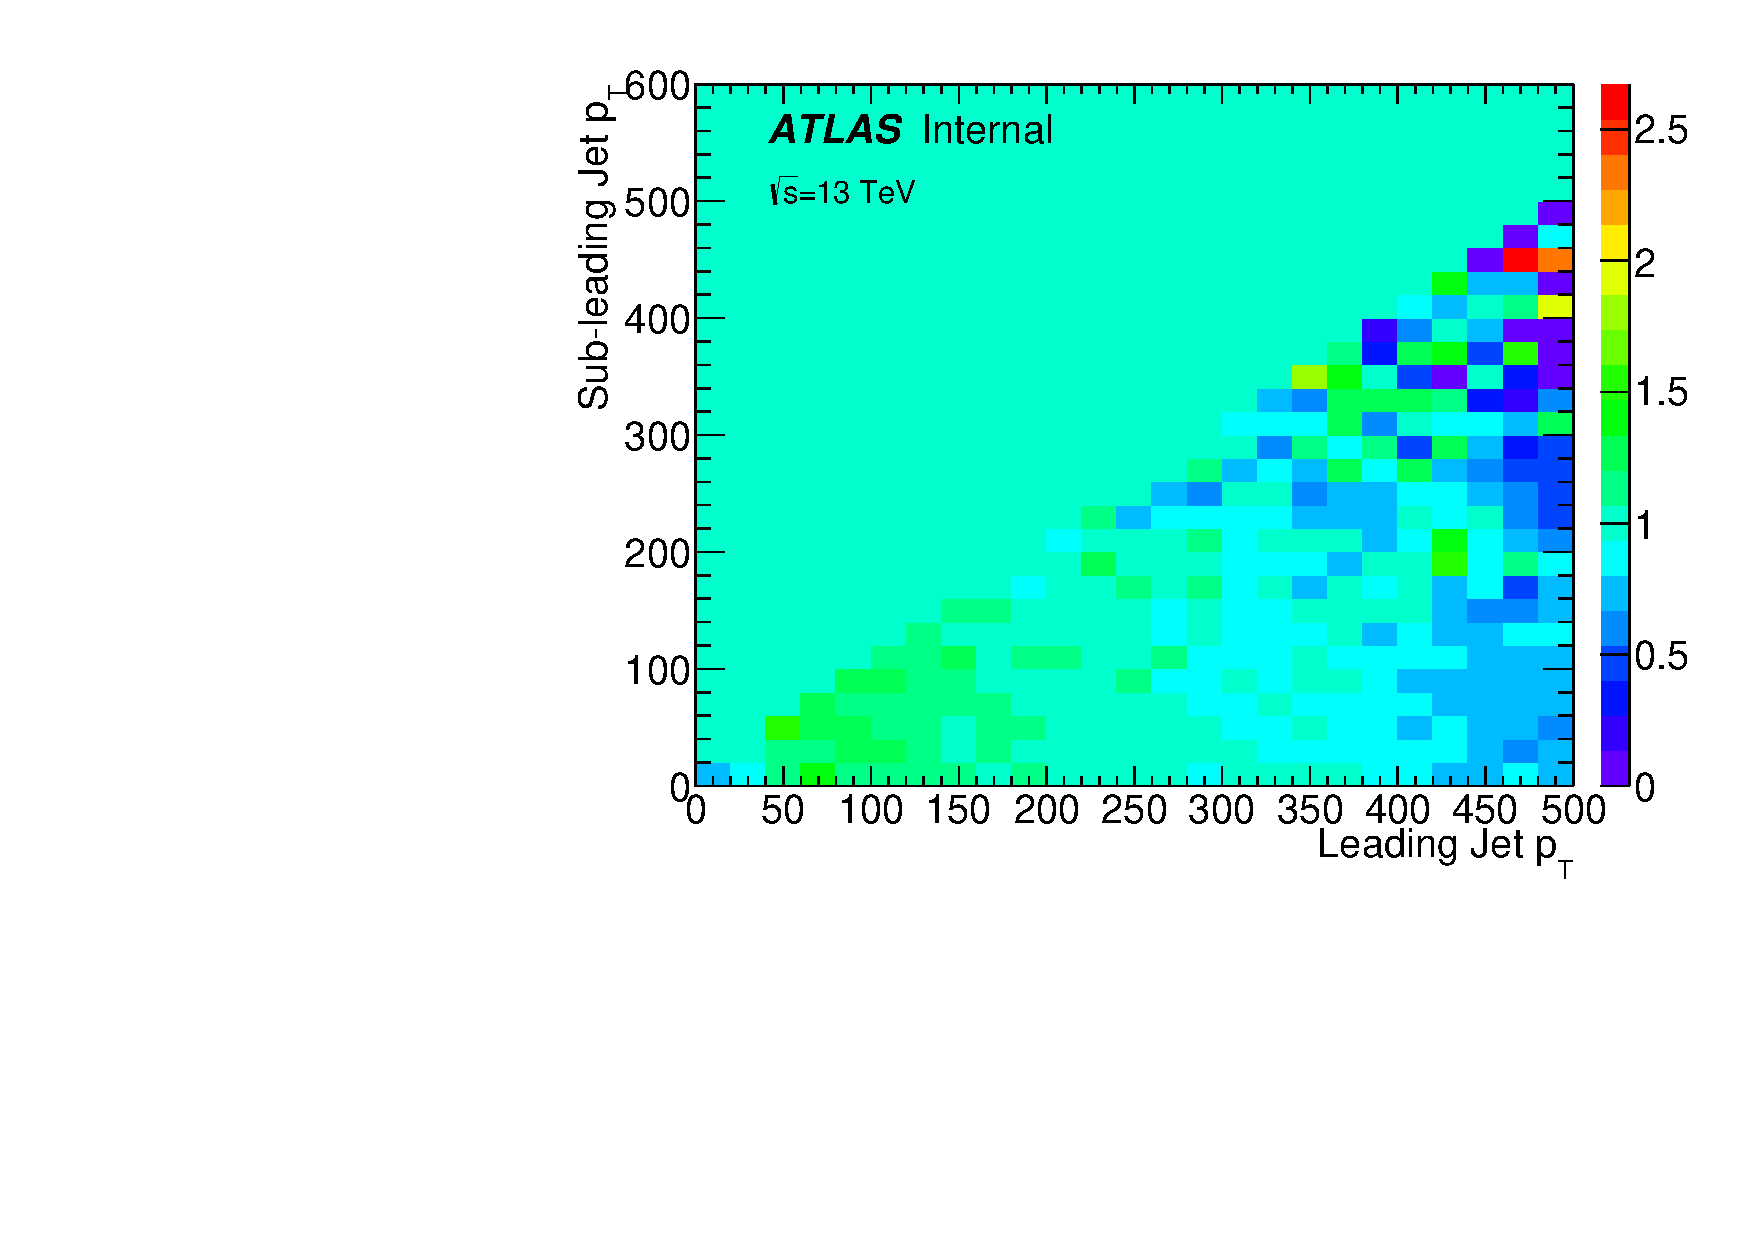
\includegraphics[width=0.6\textwidth]{figures/gbb/pTReweightMap.pdf}
\caption{The re-weighting factor applied to MC as a function of leading and sub-leading track jet \pt.}
  \label{fig:gbb-reweightmap}
\end{figure}


\begin{figure}[htbp]
  \centering
 %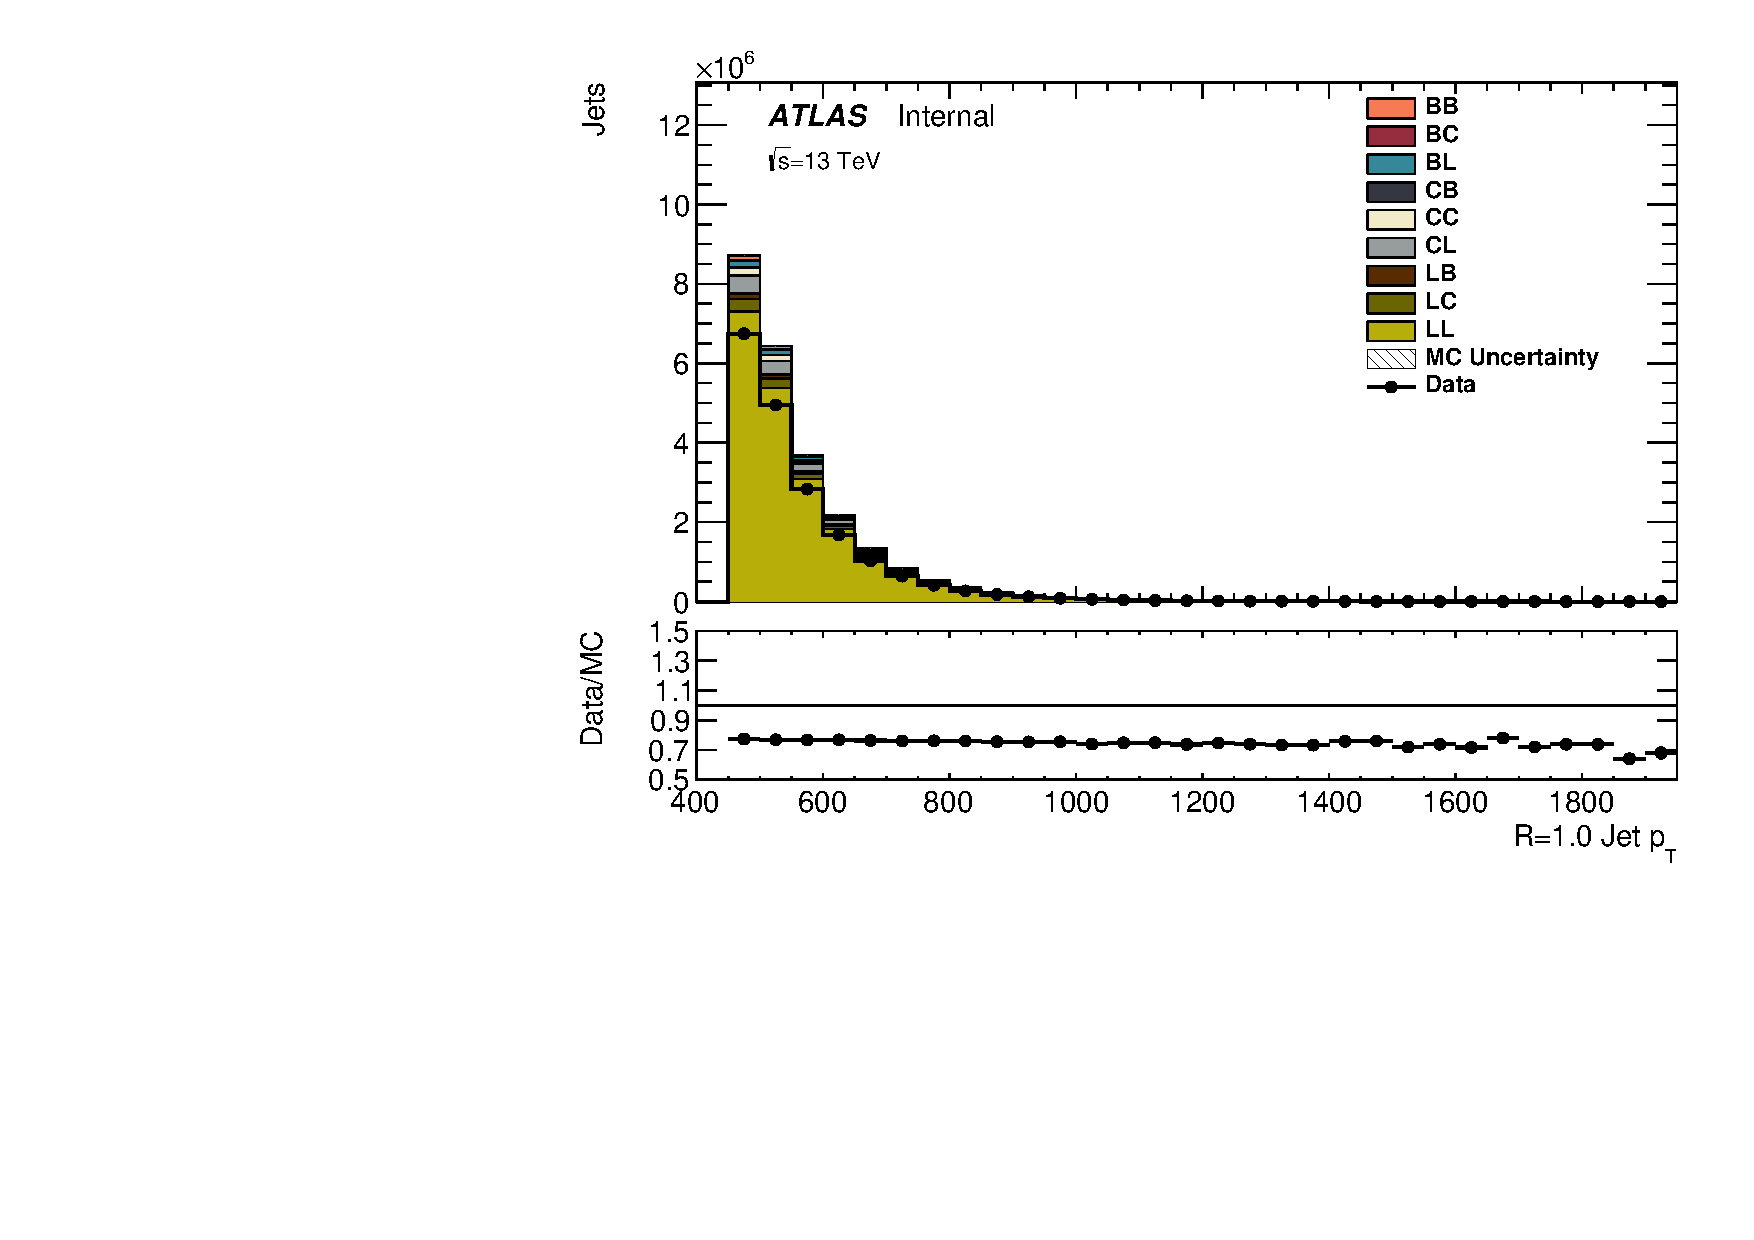
\includegraphics[width=0.38\textwidth]{figures/gbb/LargeRJet_pT_NoReweight.pdf}
 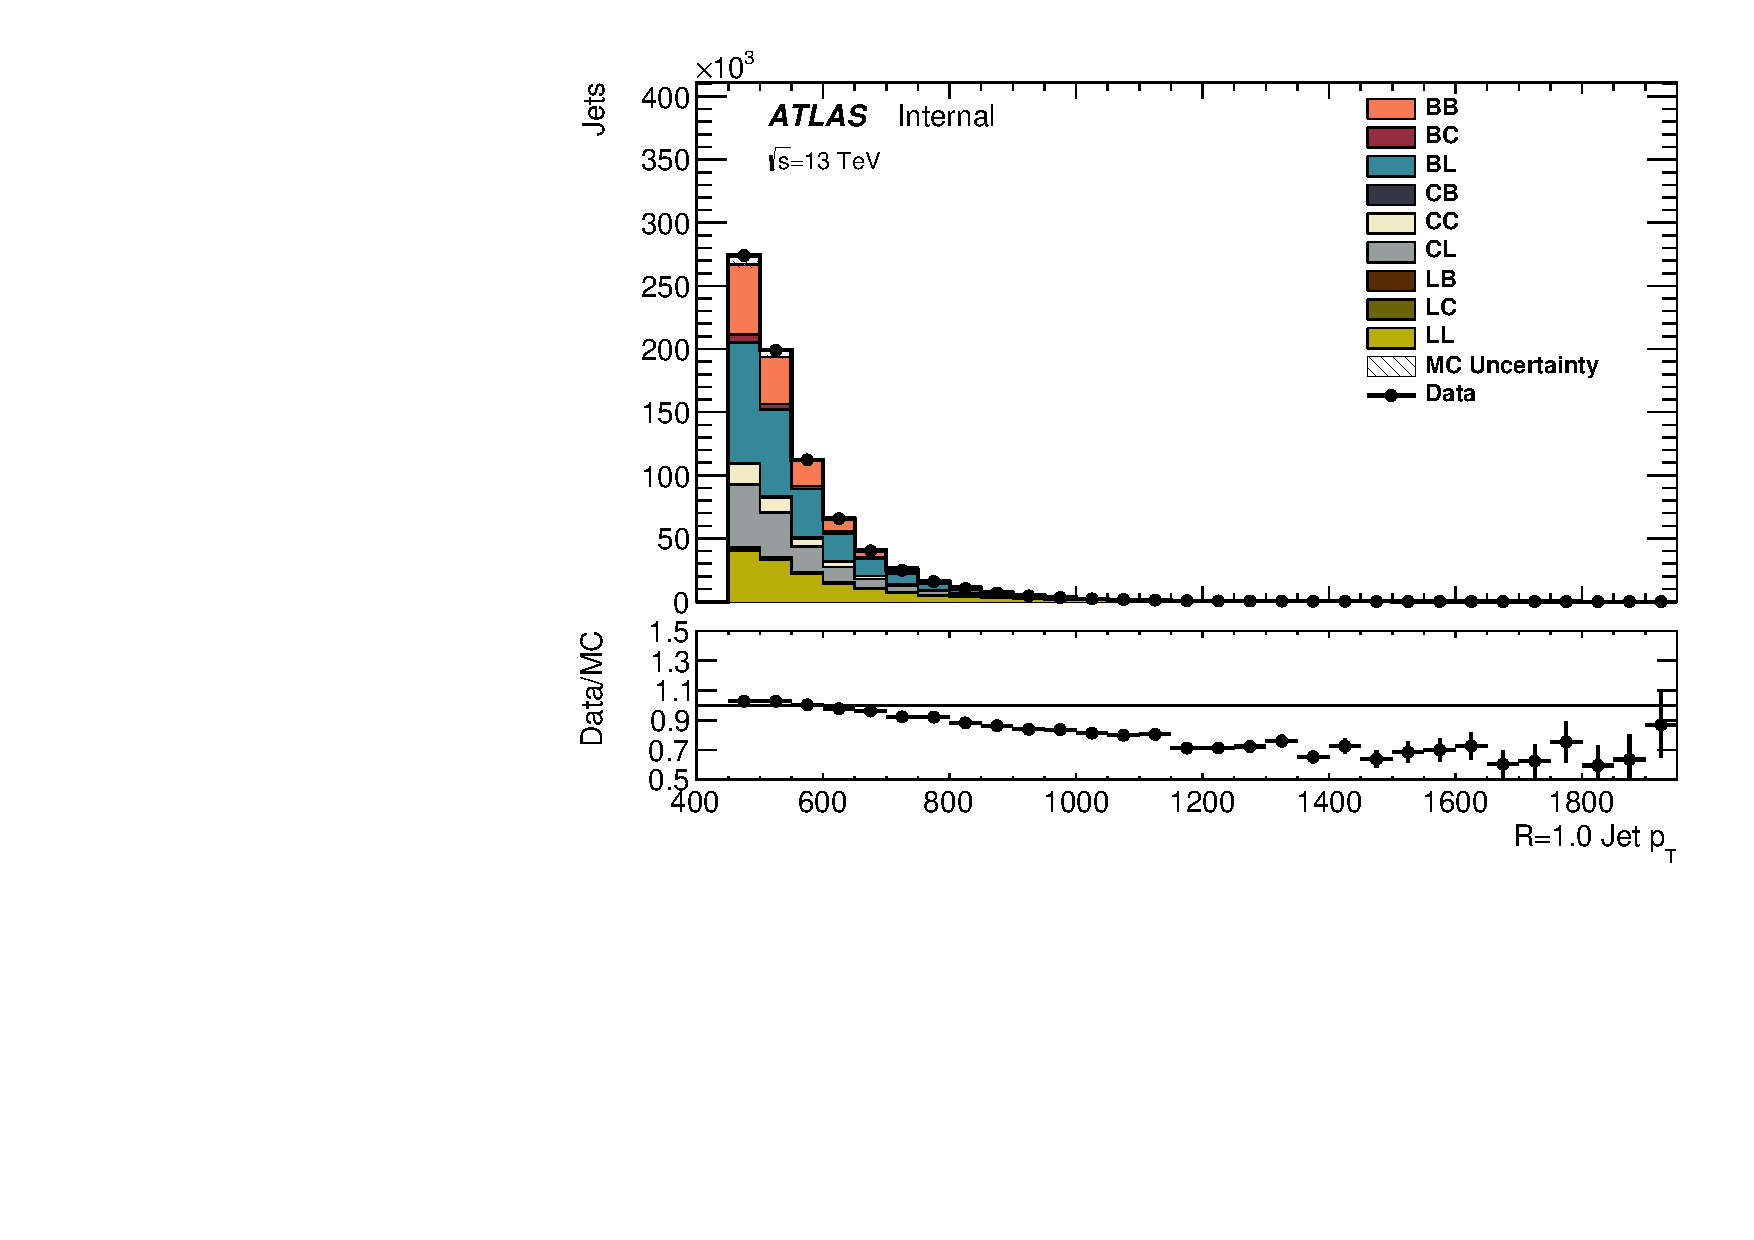
\includegraphics[width=0.38\textwidth]{figures/gbb/LargeRJet_pT_PreReweight.pdf}
 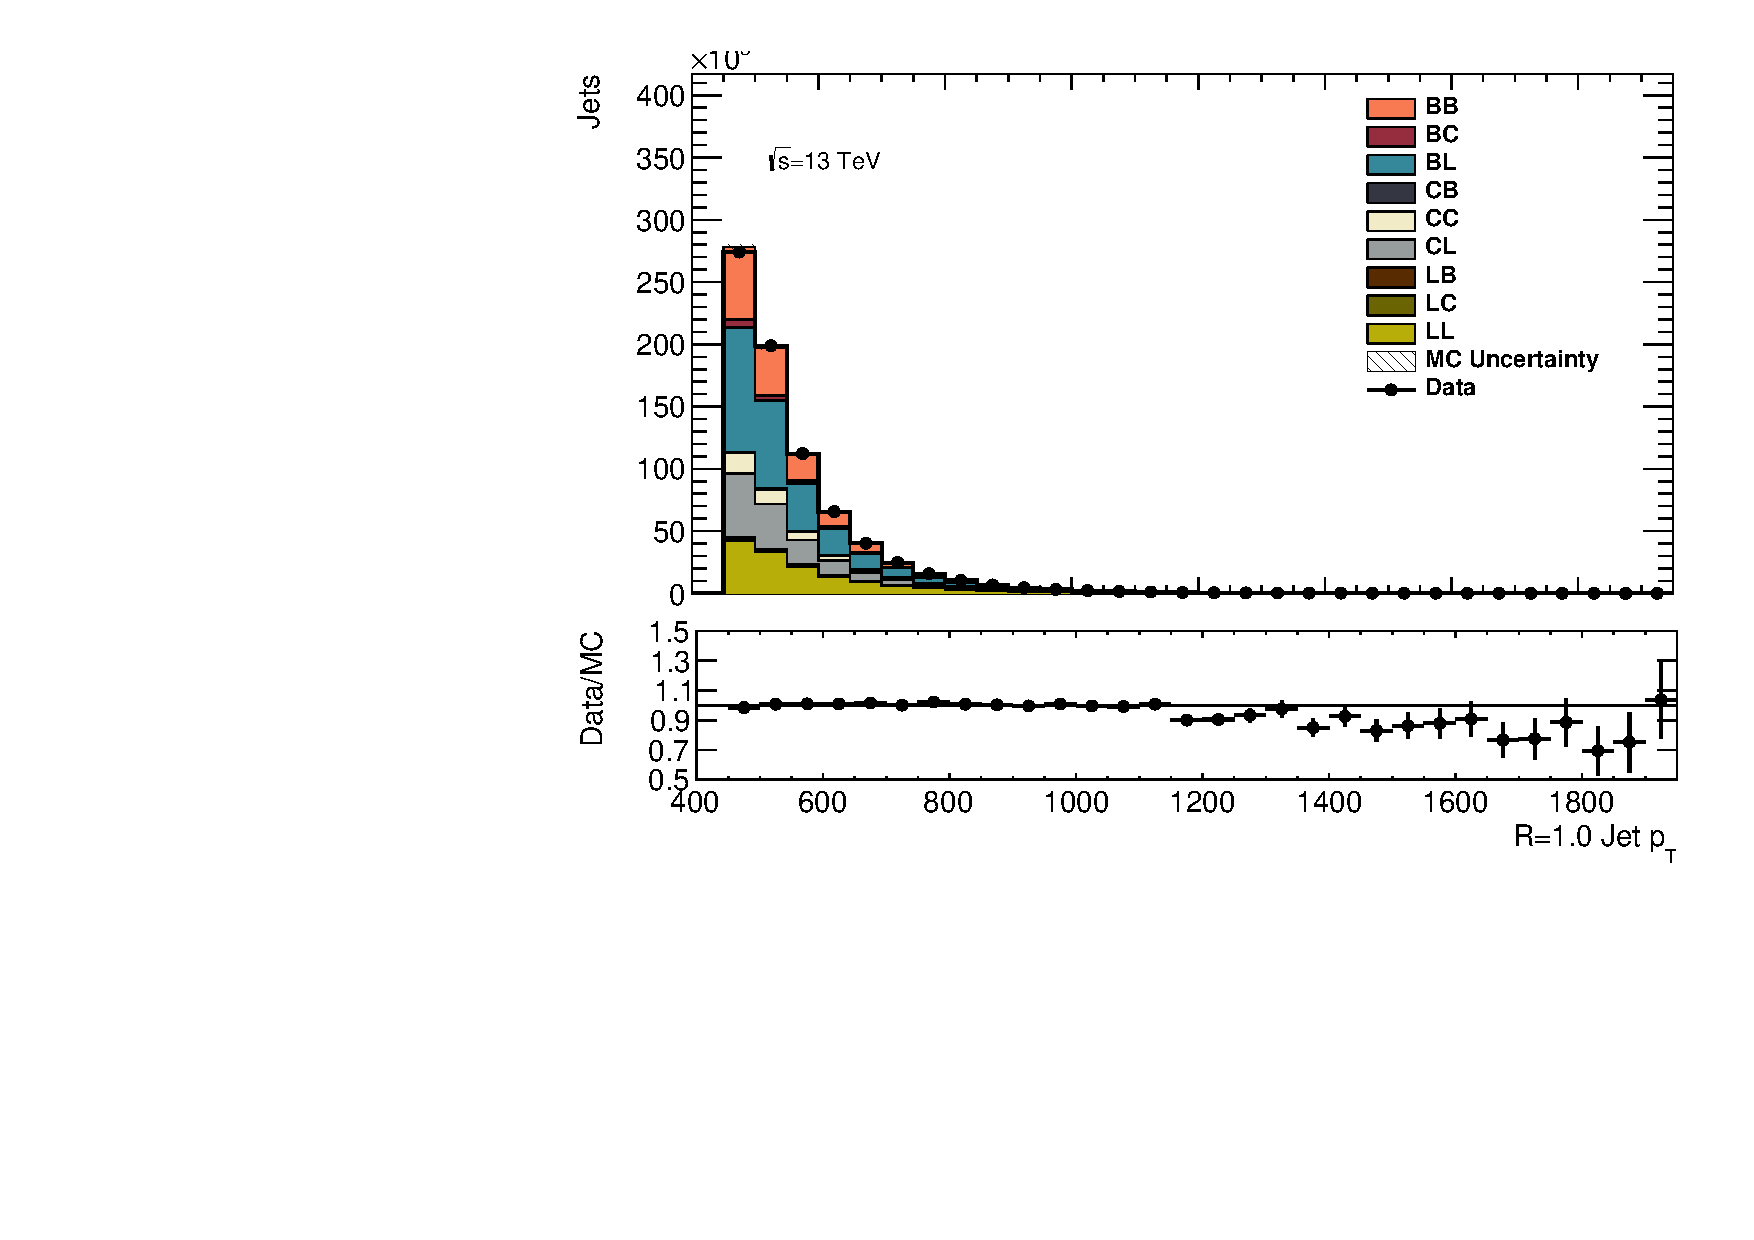
\includegraphics[width=0.38\textwidth]{figures/gbb/LargeRJet_pT_Reweight.pdf}
\caption{Data/MC comparison of $R=1.0$ jet post $b$-tagging without kinematic re-weighting (left) and post $b$-tagging with kinematic re-weighting (right).}% The label of the $R=1.0$ jet flavor content ``XY'' denotes the leading and sub-leading track jet flavor. For example, the flavors of the leading and sub-leading track jet of a ``BL'' $R=1.0$ jet are `B' and `Light' respectively.}
  \label{fig:gbb-pT_largeR}
\end{figure}


\begin{figure}[htbp]
  \centering
  %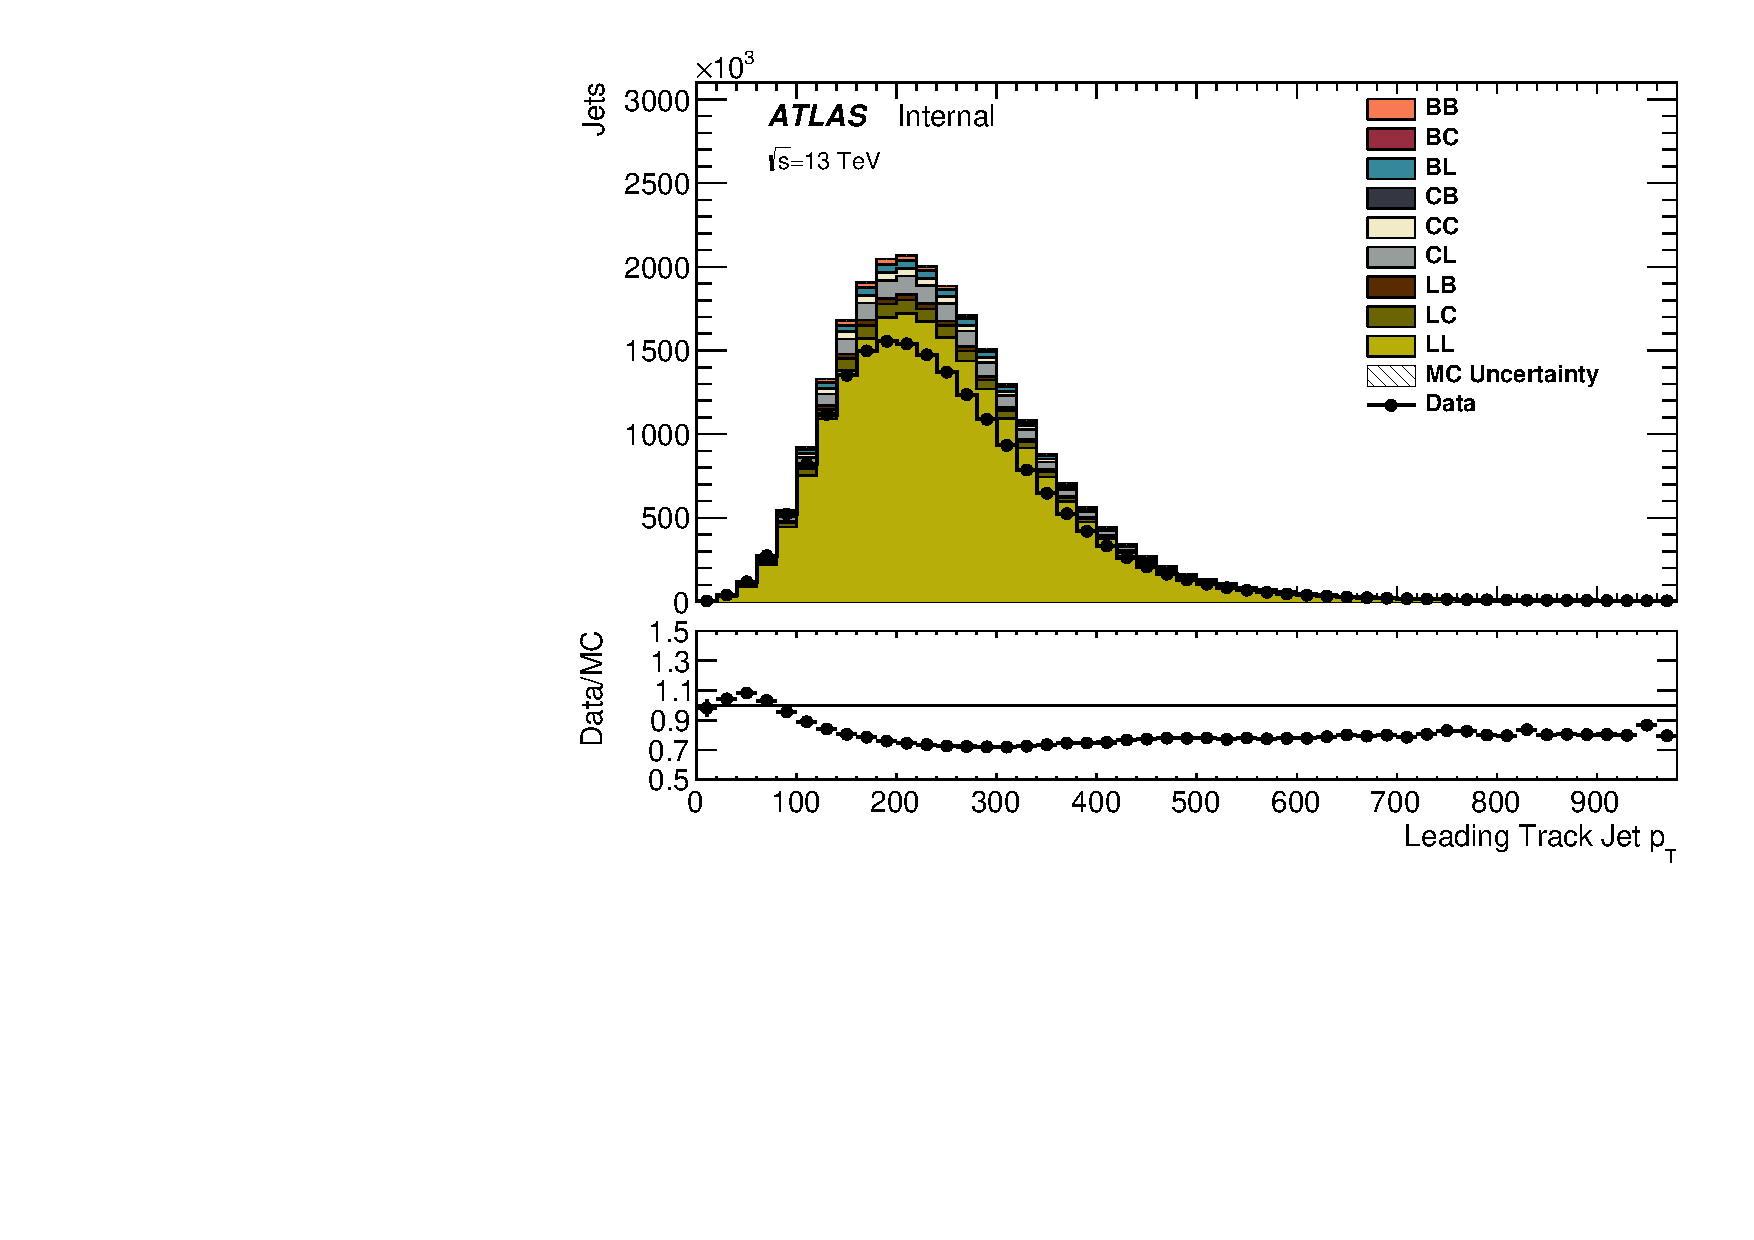
\includegraphics[width=0.38\textwidth]{figures/gbb/LeadTrkJet_pT_NoReweight.pdf}
 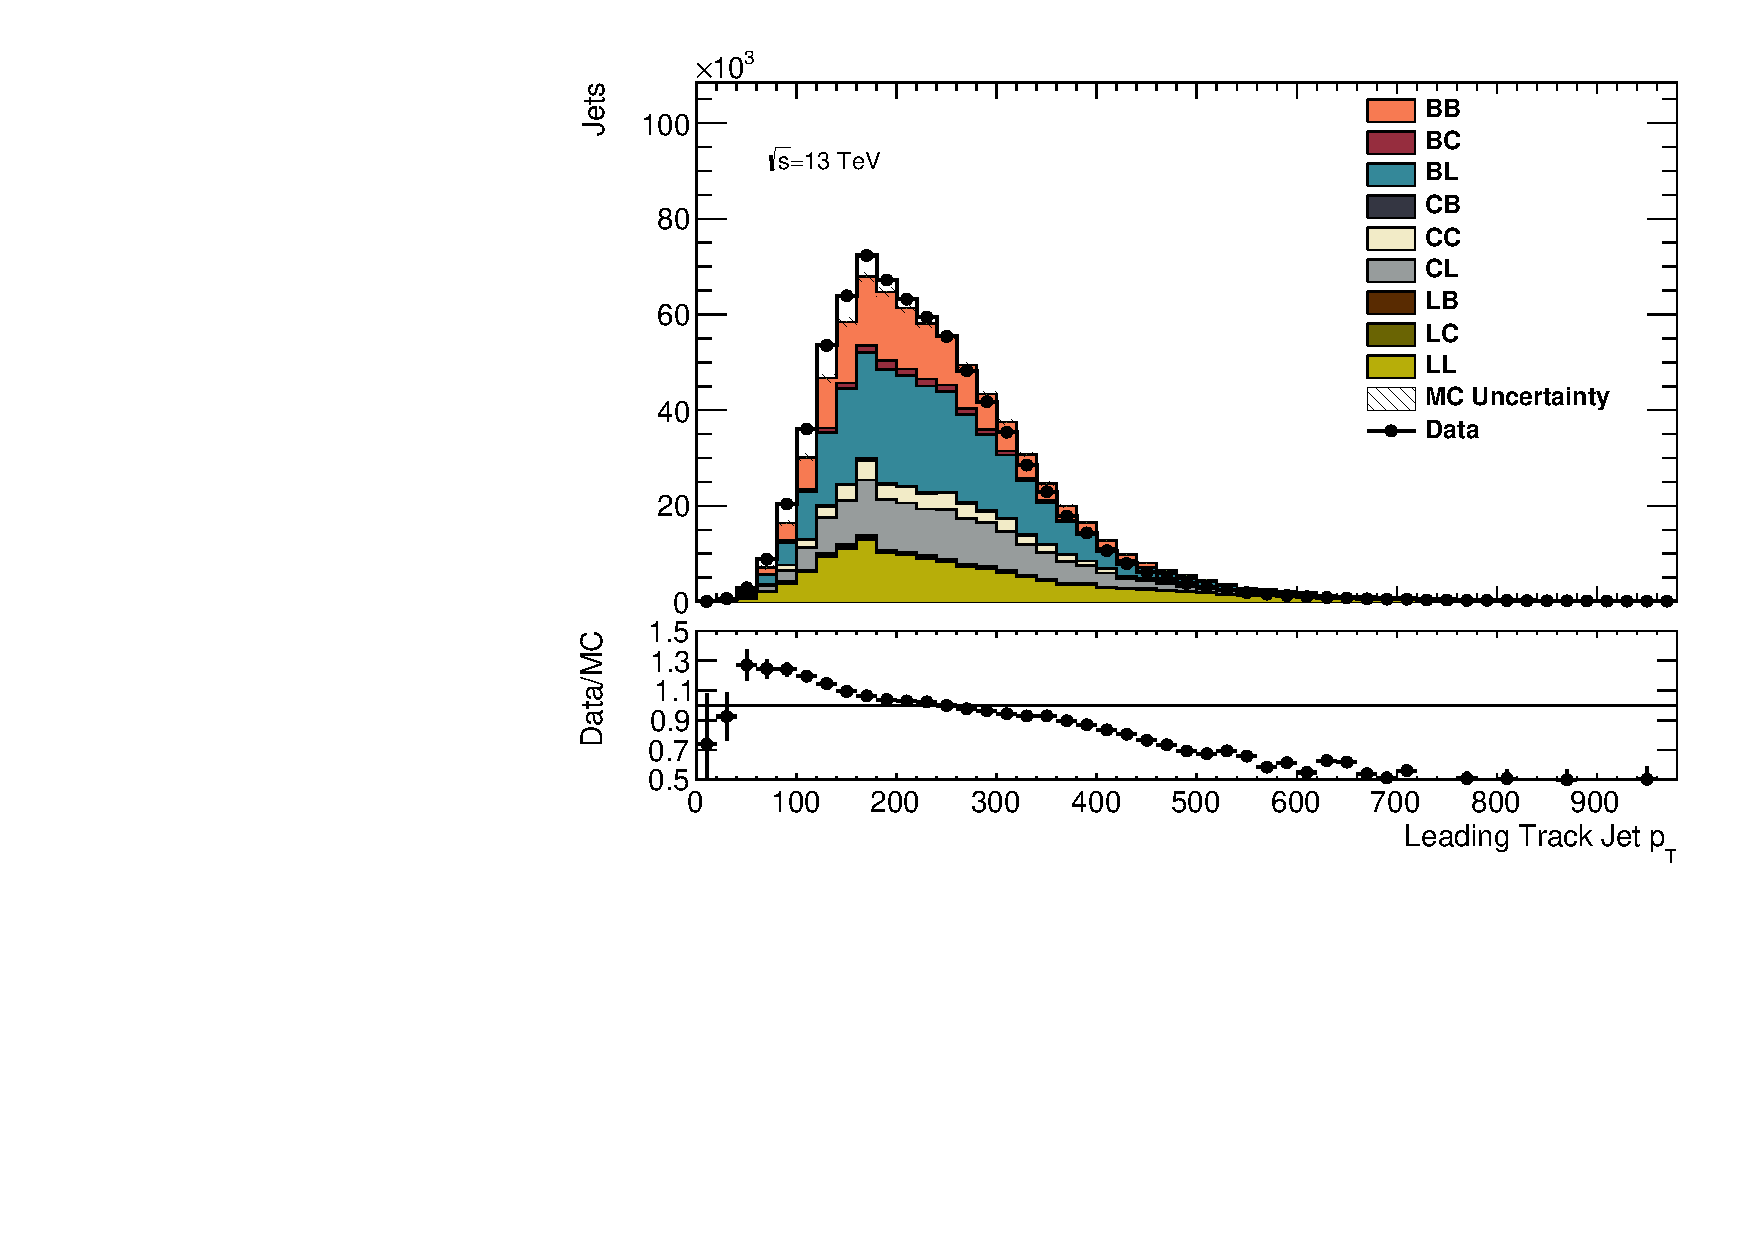
\includegraphics[width=0.38\textwidth]{figures/gbb/LeadTrkJet_pT_PreReweight.pdf}
 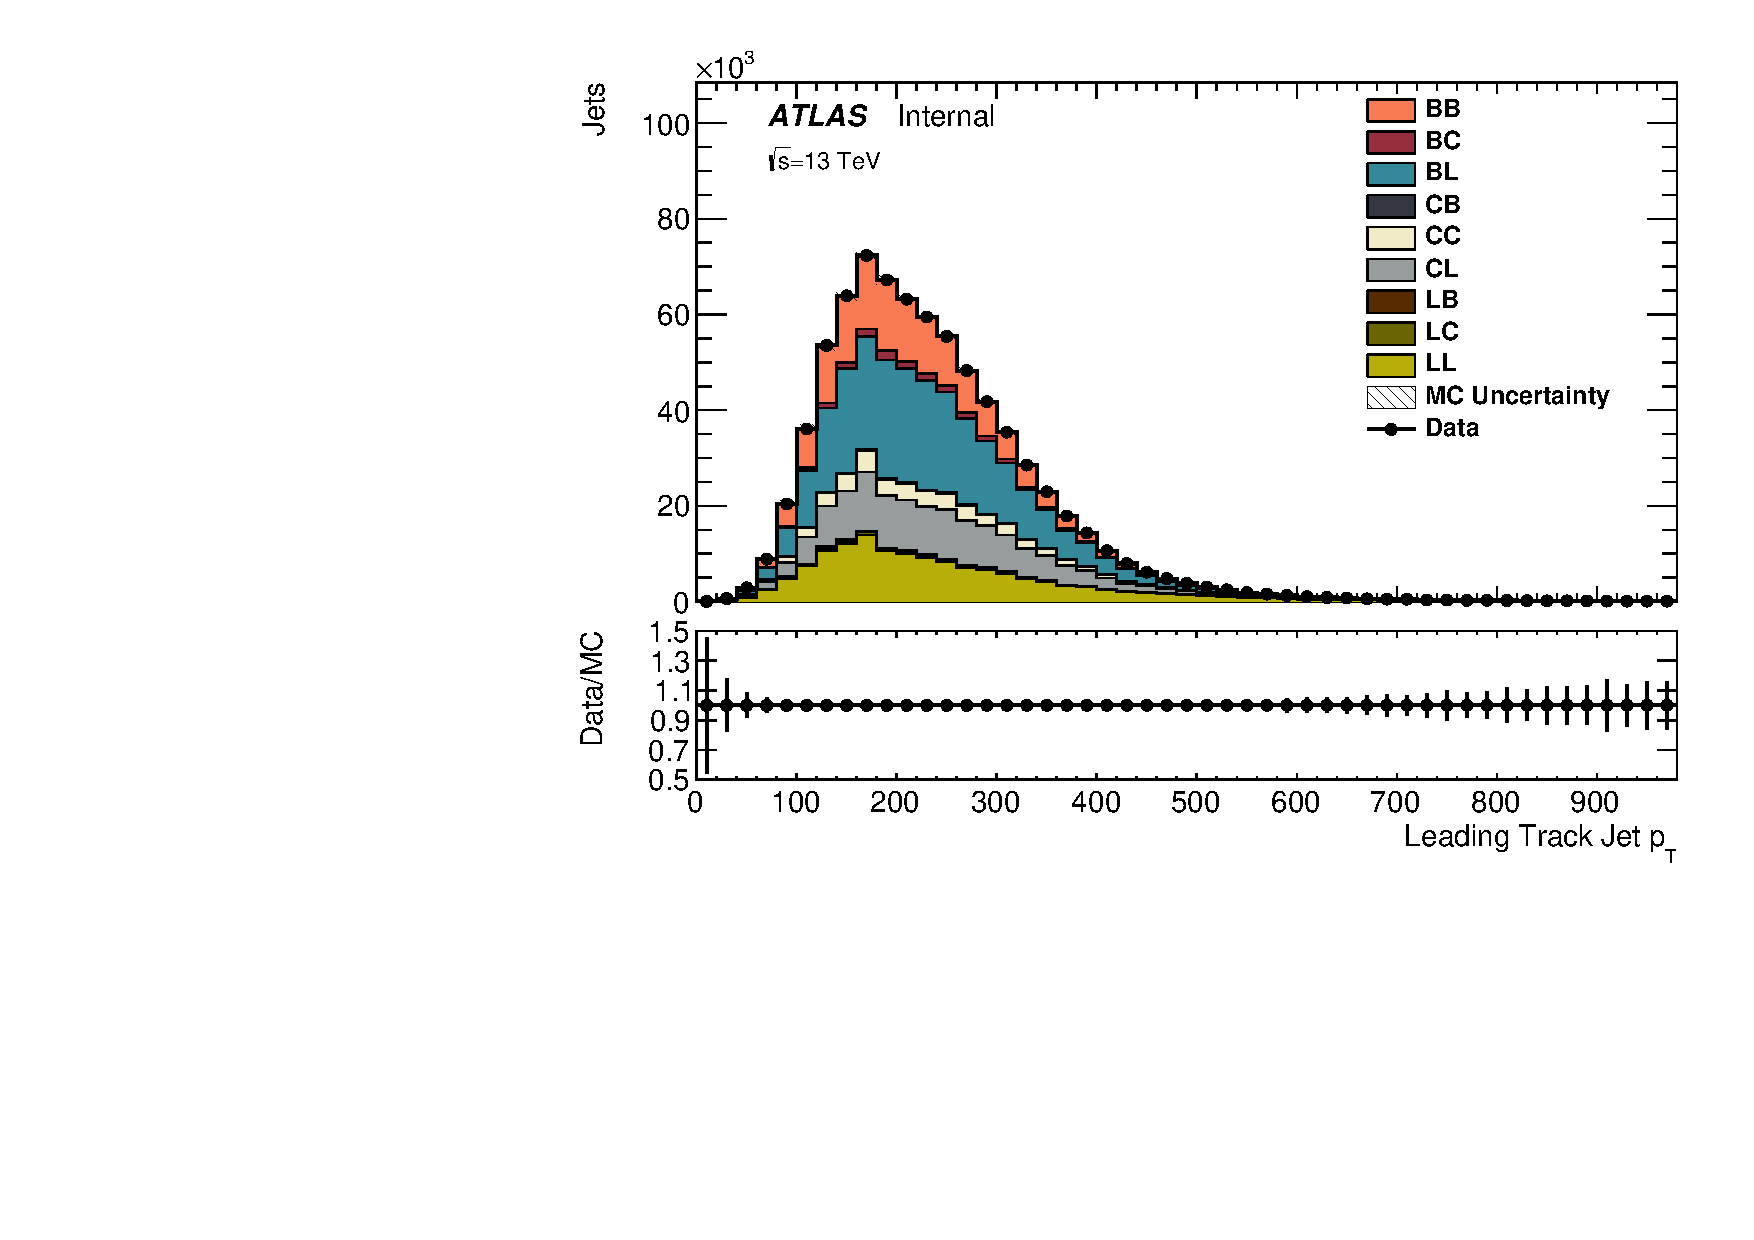
\includegraphics[width=0.38\textwidth]{figures/gbb/LeadTrkJet_pT_Reweight.pdf}
\caption{Data/MC comparison of leading track jets \pt post $b$-tagging without kinematic re-weighting (left) and post $b$-tagging with kinematic re-weighting (right).} % The label of the $R=1.0$ jet flavor content ``XY'' denotes the leading and sub-leading track jet flavor. For example, the flavors of the leading and sub-leading track jet of a ``BL'' $R=1.0$ jet are `B' and `Light' respectively.}
  \label{fig:gbb-pT_leadtrkjets}
\end{figure}


\begin{figure}[htbp]
  \centering
%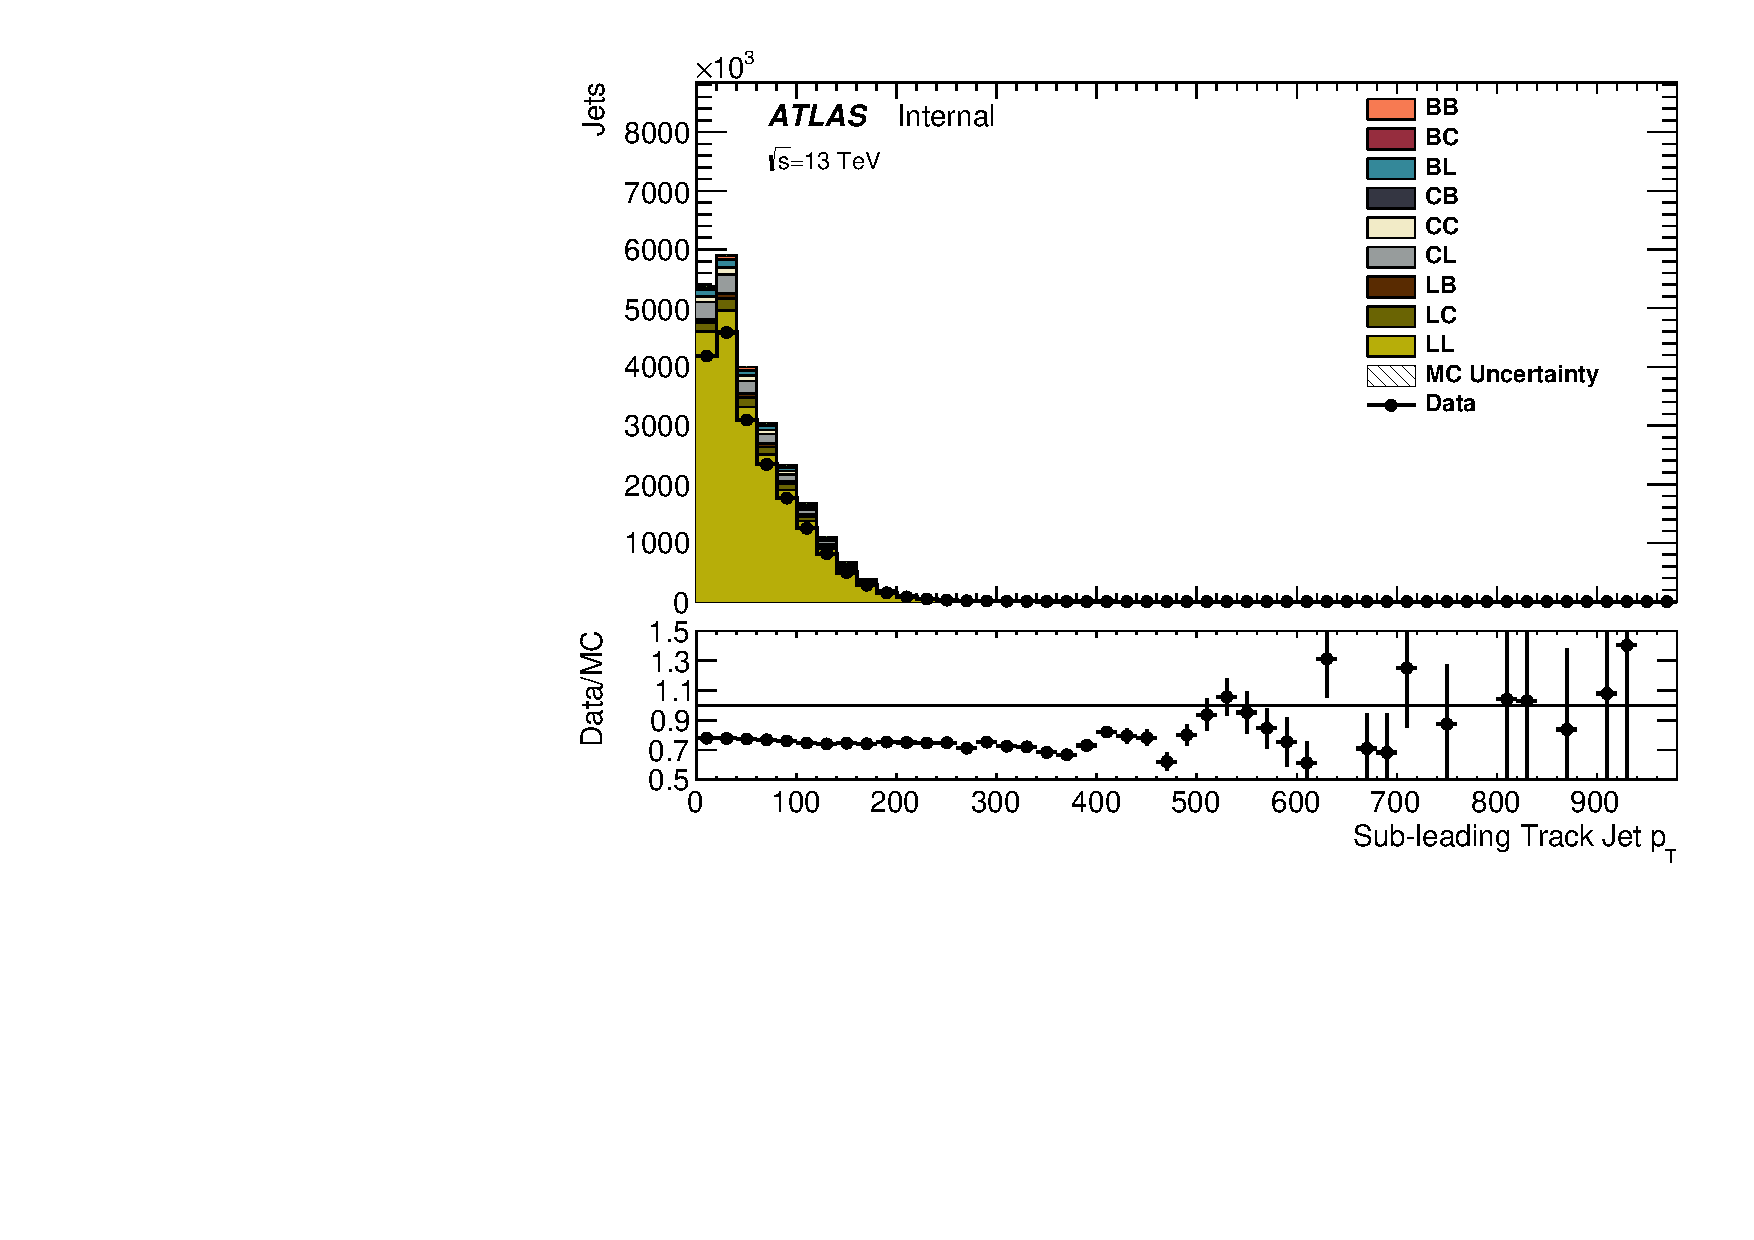
\includegraphics[width=0.38\textwidth]{figures/gbb/SubLeadTrkJet_pT_NoReweight.pdf}
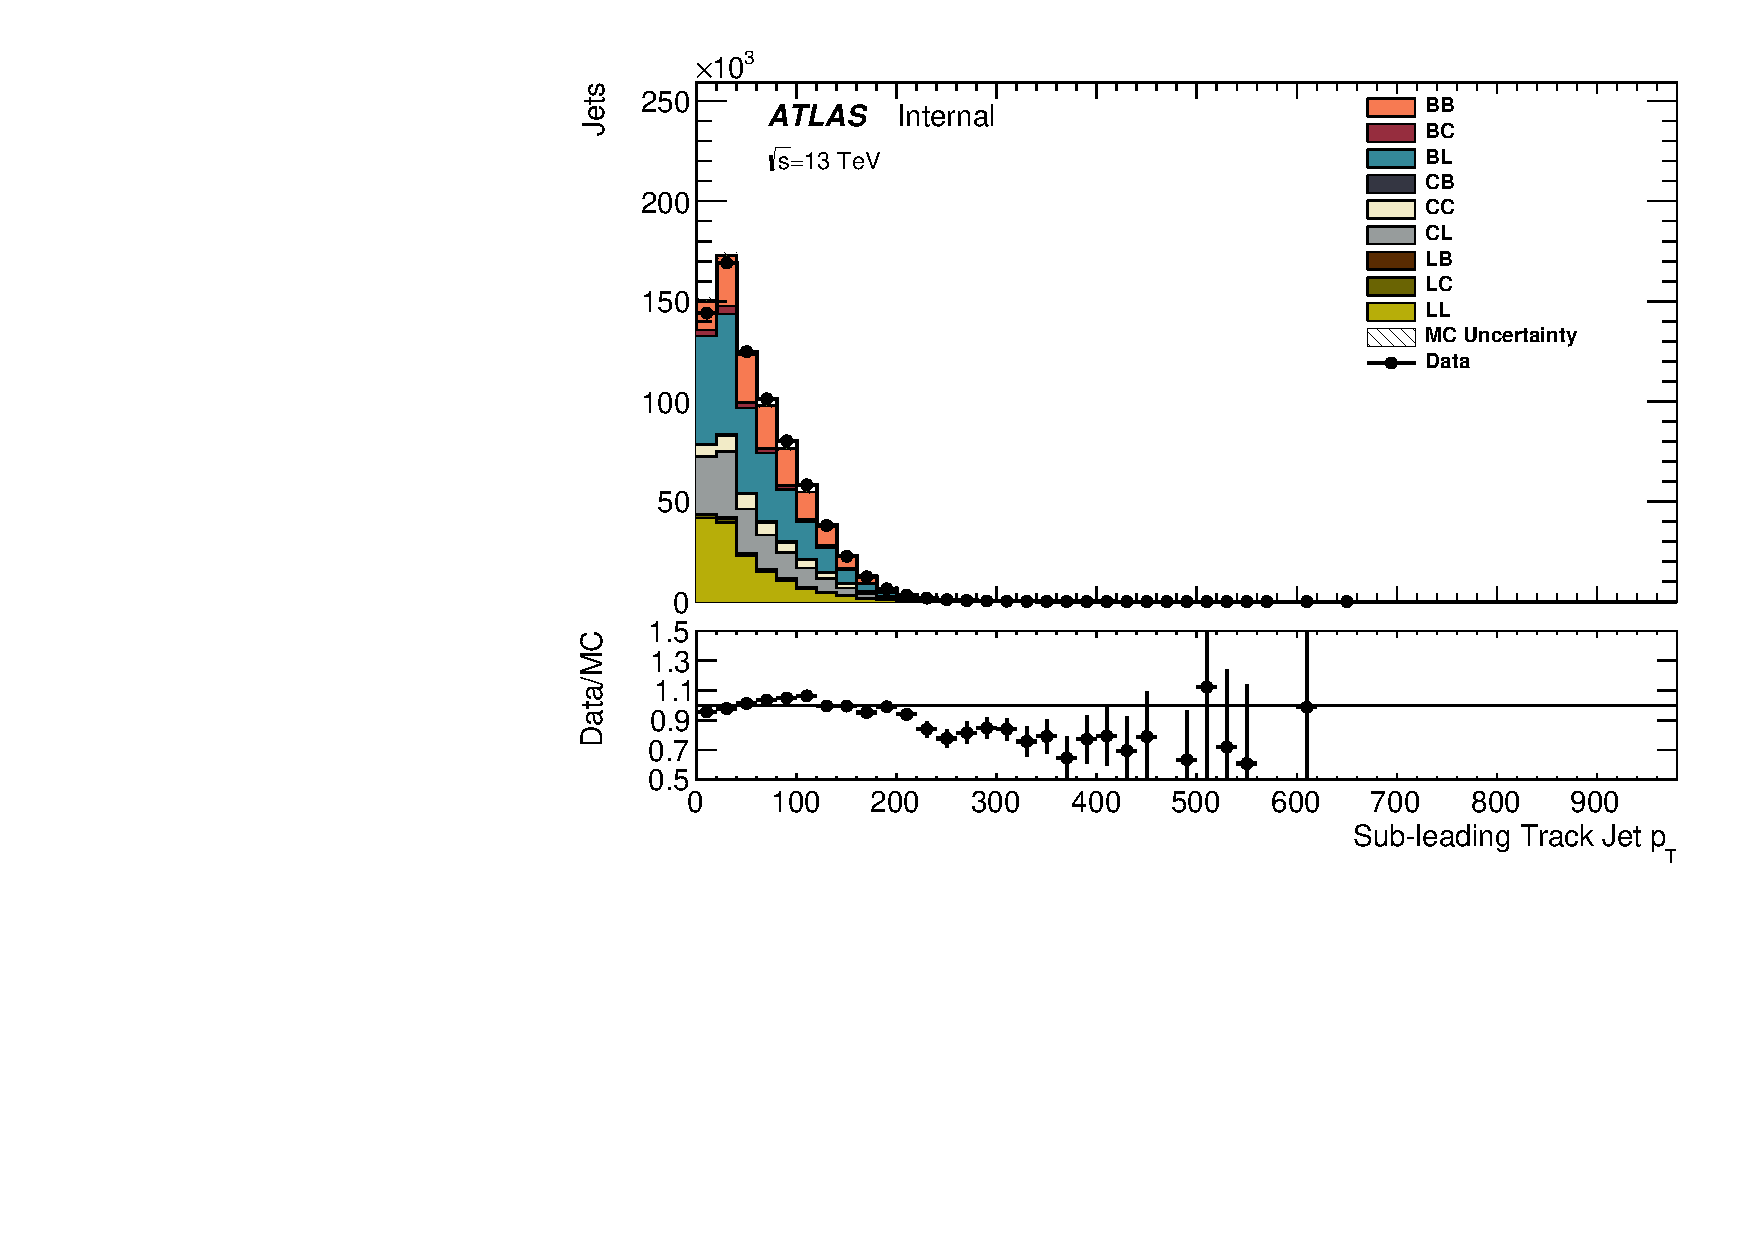
\includegraphics[width=0.38\textwidth]{figures/gbb/SubLeadTrkJet_pT_PreReweight.pdf}
 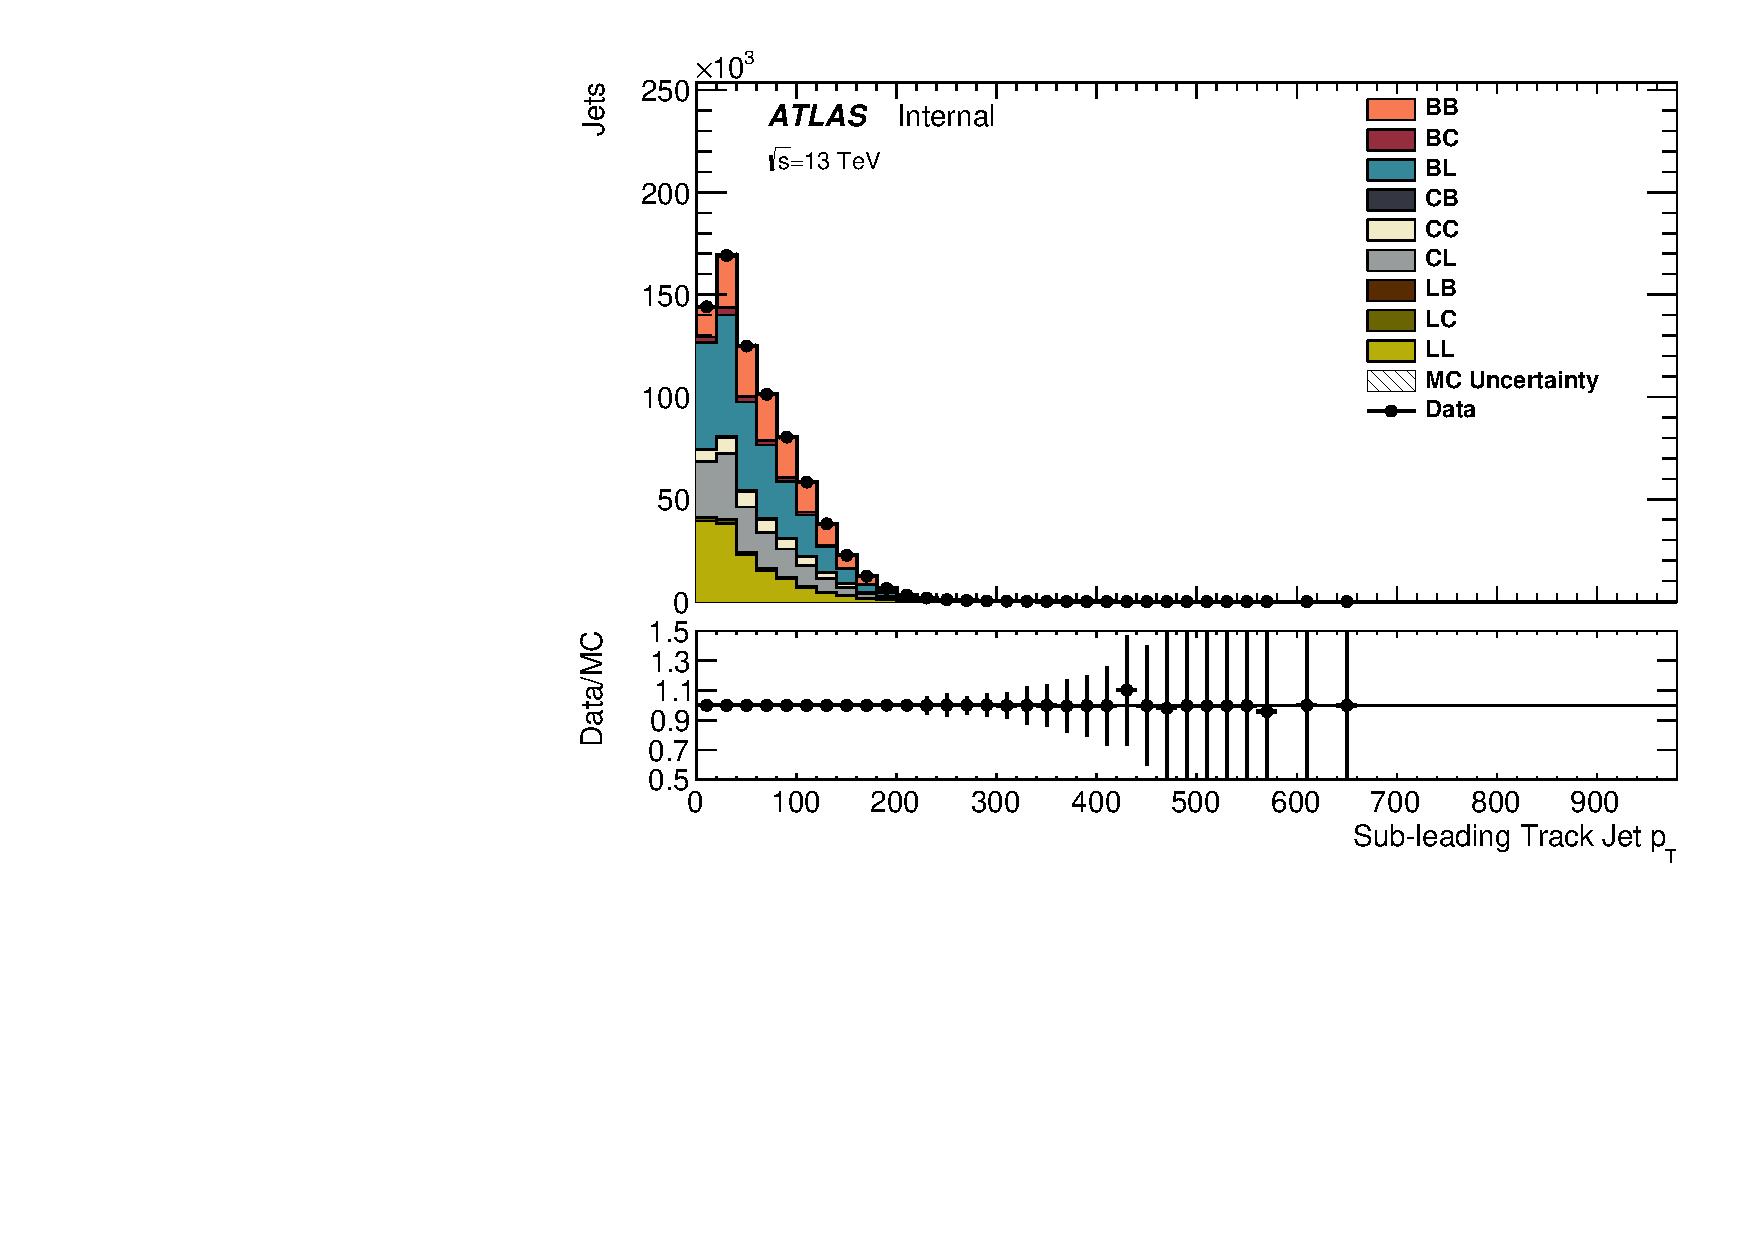
\includegraphics[width=0.38\textwidth]{figures/gbb/SubLeadTrkJet_pT_Reweight.pdf}
\caption{Data/MC comparison of sub-leading track jets \pt post $b$-tagging without kinematic re-weighting (left) and post $b$-tagging with kinematic re-weighting (right).}% The label of the $R=1.0$ jet flavor content ``XY'' denotes the leading and sub-leading track jet flavor. For example, the flavors of the leading and sub-leading track jet of a ``BL'' $R=1.0$ jet are `B' and `Light' respectively.}
  \label{fig:gbb-pT_subtrkjets}
\end{figure}


\clearpage

%-------------------------------------------------------------------------------
\section{Data / MC studies}
\label{sec:datamc}
%-------------------------------------------------------------------------------
\label{sec:gbb-bkgres}
%%%%%%%%%%%%%%%%%%%%%%%%%%%%%%%%%%%%

The flavor fraction fits are performed in each bin of each observable to determine the $b\bar b $ fractions in data. For \drbb, fits are performed in bins of \{[0.2, 0.25], [0.25, 0.3], [0.3, 0.4], [0.4,0.5], [0.5,0.6], [0.6,0.7]\}. For \zpt, fits are performed in bins of \{[0, 0.1], [0.1, 0.2], [0.2, 0.3], [0.3,0.4], [0.4,0.5]\}. For \mpt, fits are performed in bins of \{[-3, -2.2], [-2.2, -1.9], [-1.9, -1.5], [-1.5, -1.1], [-1.1,0]\}. For \dphi, fits are performed in bins of \{[0, $\pi/5$], [$\pi/5$, $2\pi/5$], [$2\pi/5$, $3\pi/5$], [$3\pi/5$, $4\pi/5$], [$4\pi/5$, $\pi$]\}. Examples of post-fit Data/MC comparisons for each variable are shown in Fig.~\ref{fig:fit-example-leading}~\ref{fig:fit-example-subleading}. Refer to \ref{sec:app-subsd0fits} for all pre-fits and post-fits data-MC comparisons. The MC predicted and fitted fraction of each flavor component are shown in Fig.~\ref{fig:gbb-fitfrac}.

Four sets of fit cross check are performed: (1) using \sdzero as discriminant (2) using \subsubsdzero (3) using $p_T$ parameterized templates and (4) with track jet kinematic re-weighting. The cross check results are summarized in Fig.~\ref{fig:dR-fitfrac-crosscheck}~\ref{fig:ZpT-fitfrac-crosscheck}~\ref{fig:fracmasspt-fitfrac-crosscheck}~\ref{fig:dphi-fitfrac-crosscheck}. We observe closure of the fitted signal (`BB' component) event fraction in all the cross checks within fitting uncertainties. The size of each of the systematic uncertainty is summarized in Table ~\ref{tab:dRsys}~\ref{tab:ZpTsys}~\ref{tab:fracmassptsys}~\ref{tab:dphisys}.

\begin{figure}[htbp]
  \centering
 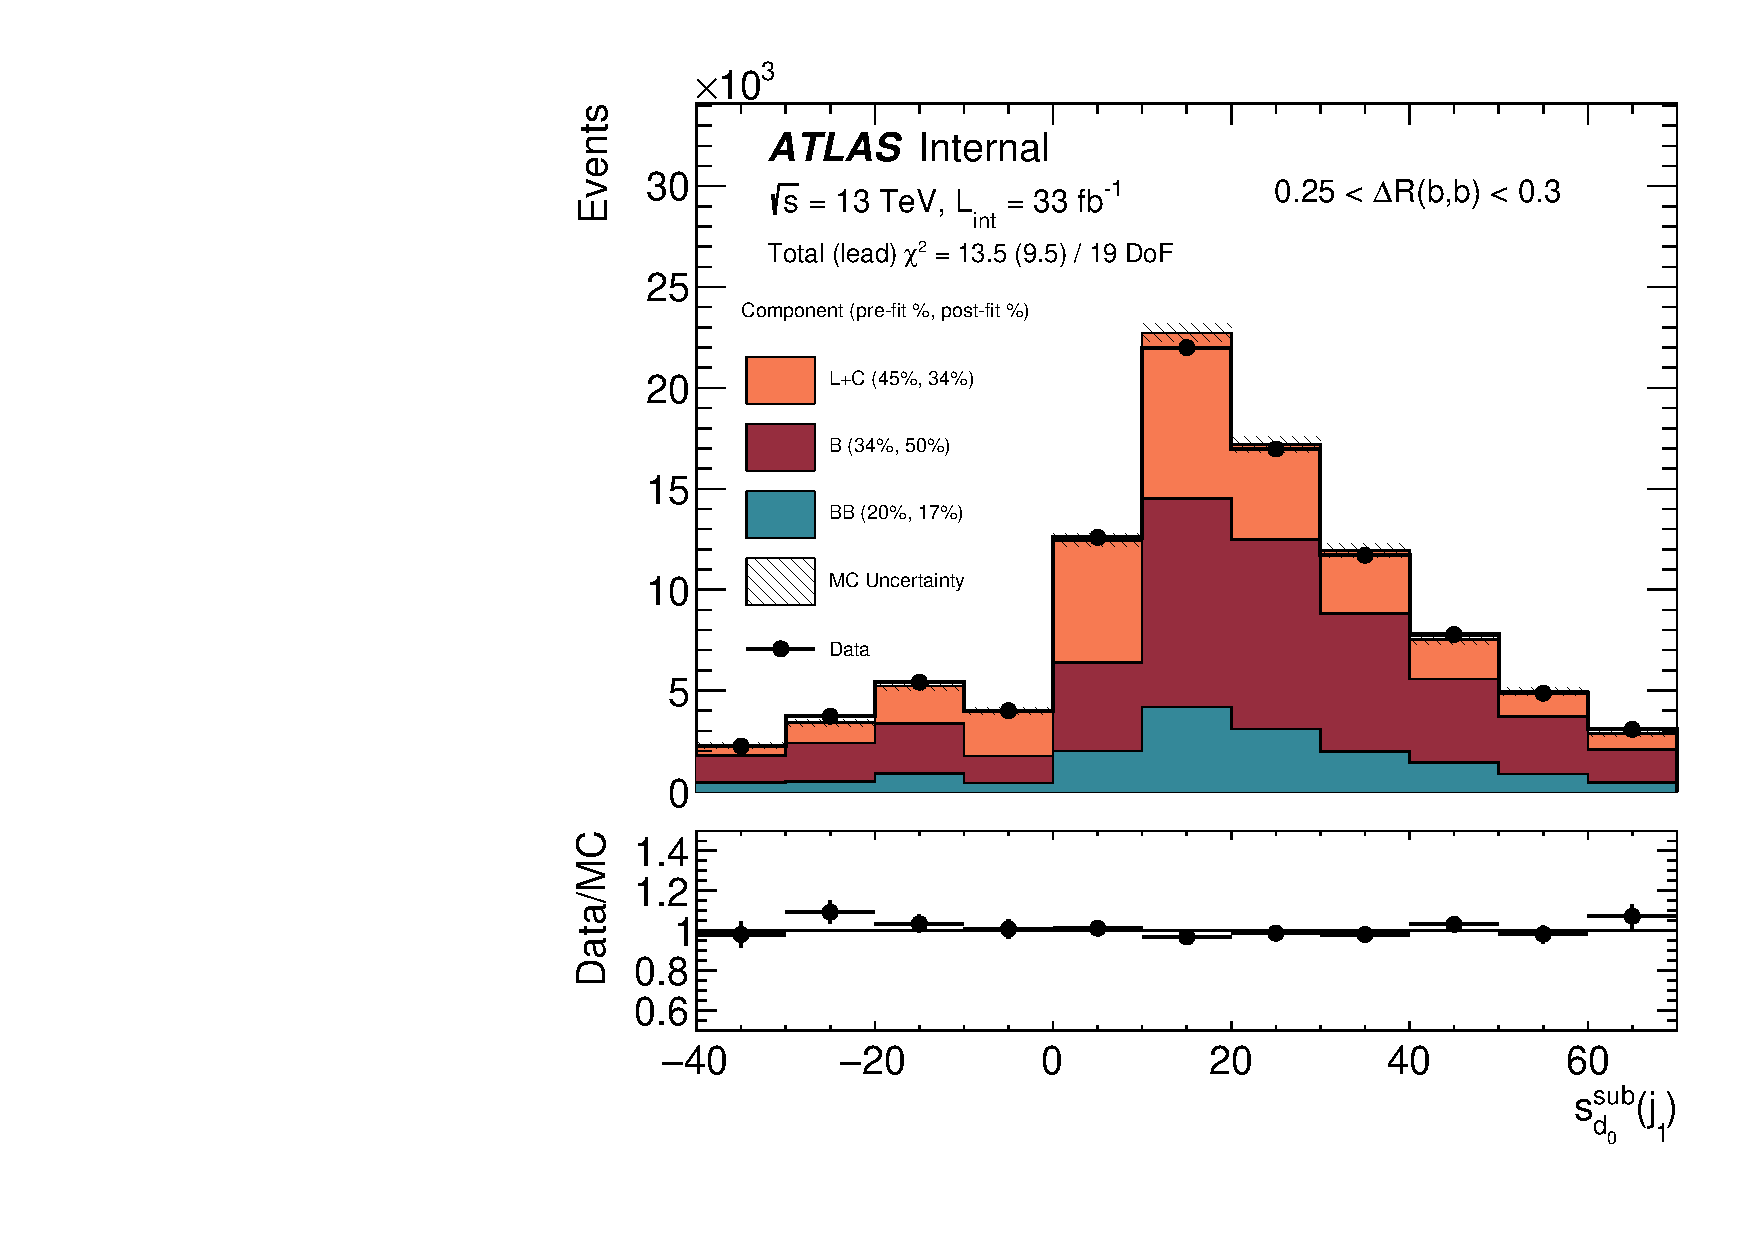
\includegraphics[width=0.45\textwidth]{figures/gbb/paperplots/Canv_Fit_dR_LpT_INF_SpT_INF_coarse_x}
 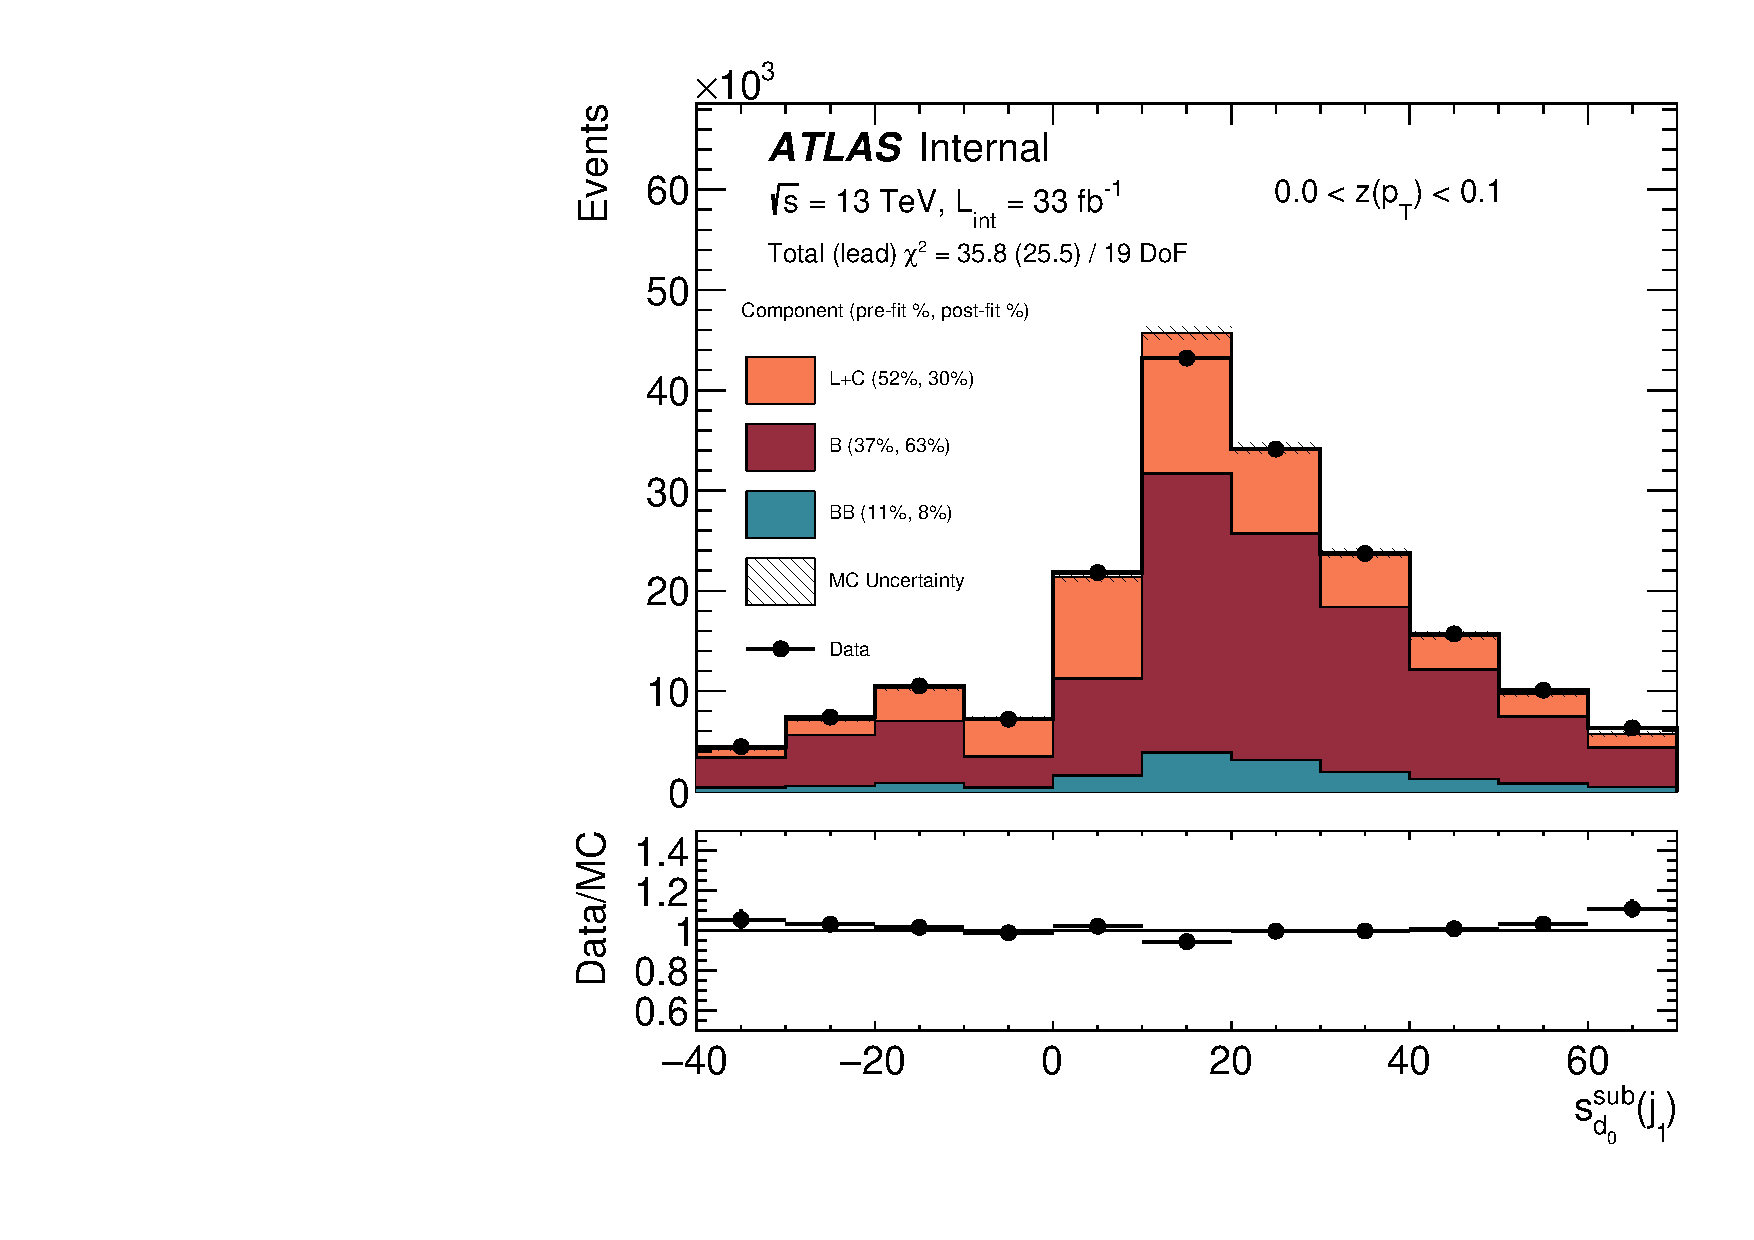
\includegraphics[width=0.45\textwidth]{figures/gbb/paperplots/Canv_Fit_zpt_LpT_INF_SpT_INF_coarse_x}  
 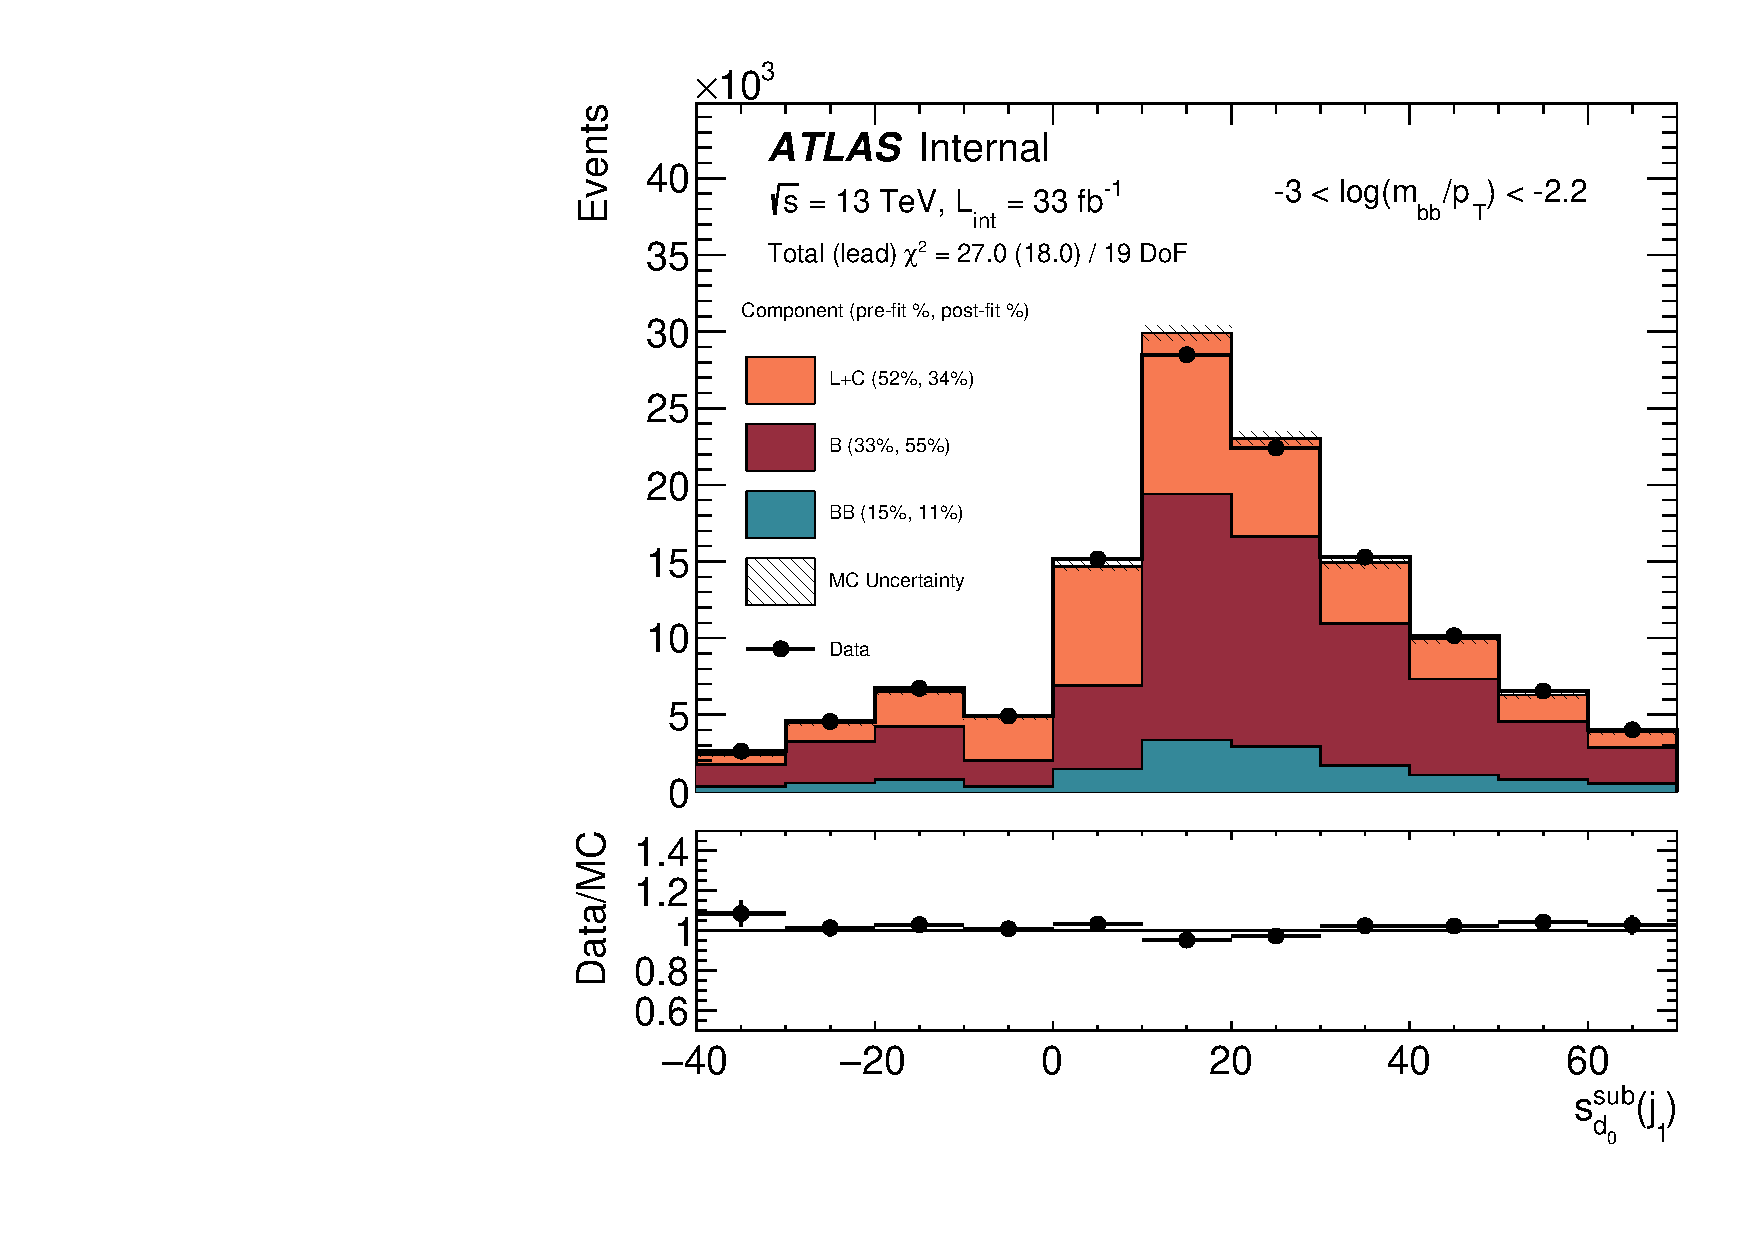
\includegraphics[width=0.45\textwidth]{figures/gbb/paperplots/Canv_Fit_M_LpT_INF_SpT_INF_coarse_x}
 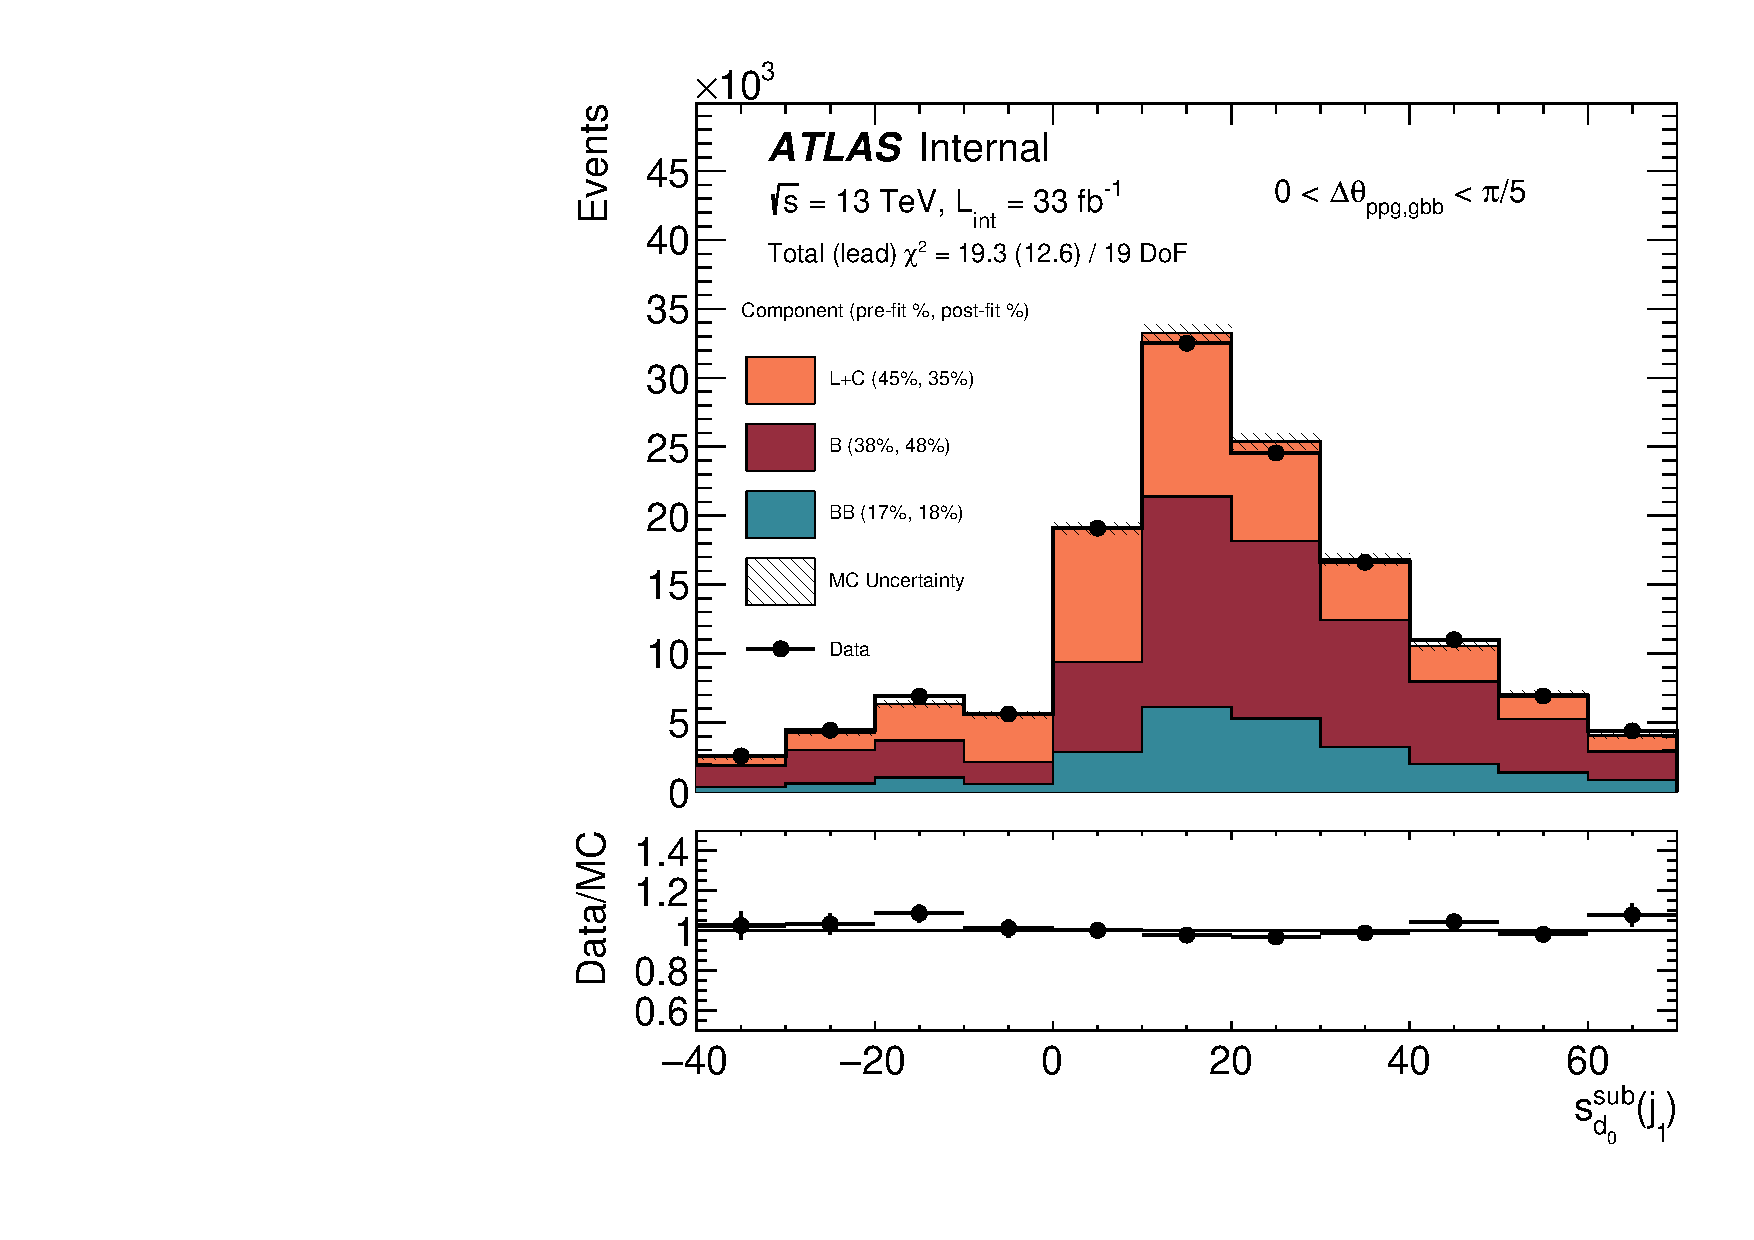
\includegraphics[width=0.45\textwidth]{figures/gbb/paperplots/Canv_Fit_dphi_LpT_INF_SpT_INF_coarse_x}
\caption{Example of post-fit \subsdzero distributions of the leading track jets in bin of \drbb (top left), \zpt (top right), \mpt (bottom left) and \dphi (bottom right). Error bars only include statistical uncertainties.}
  \label{fig:fit-example-leading}
\end{figure}


\begin{figure}[htbp]
  \centering
 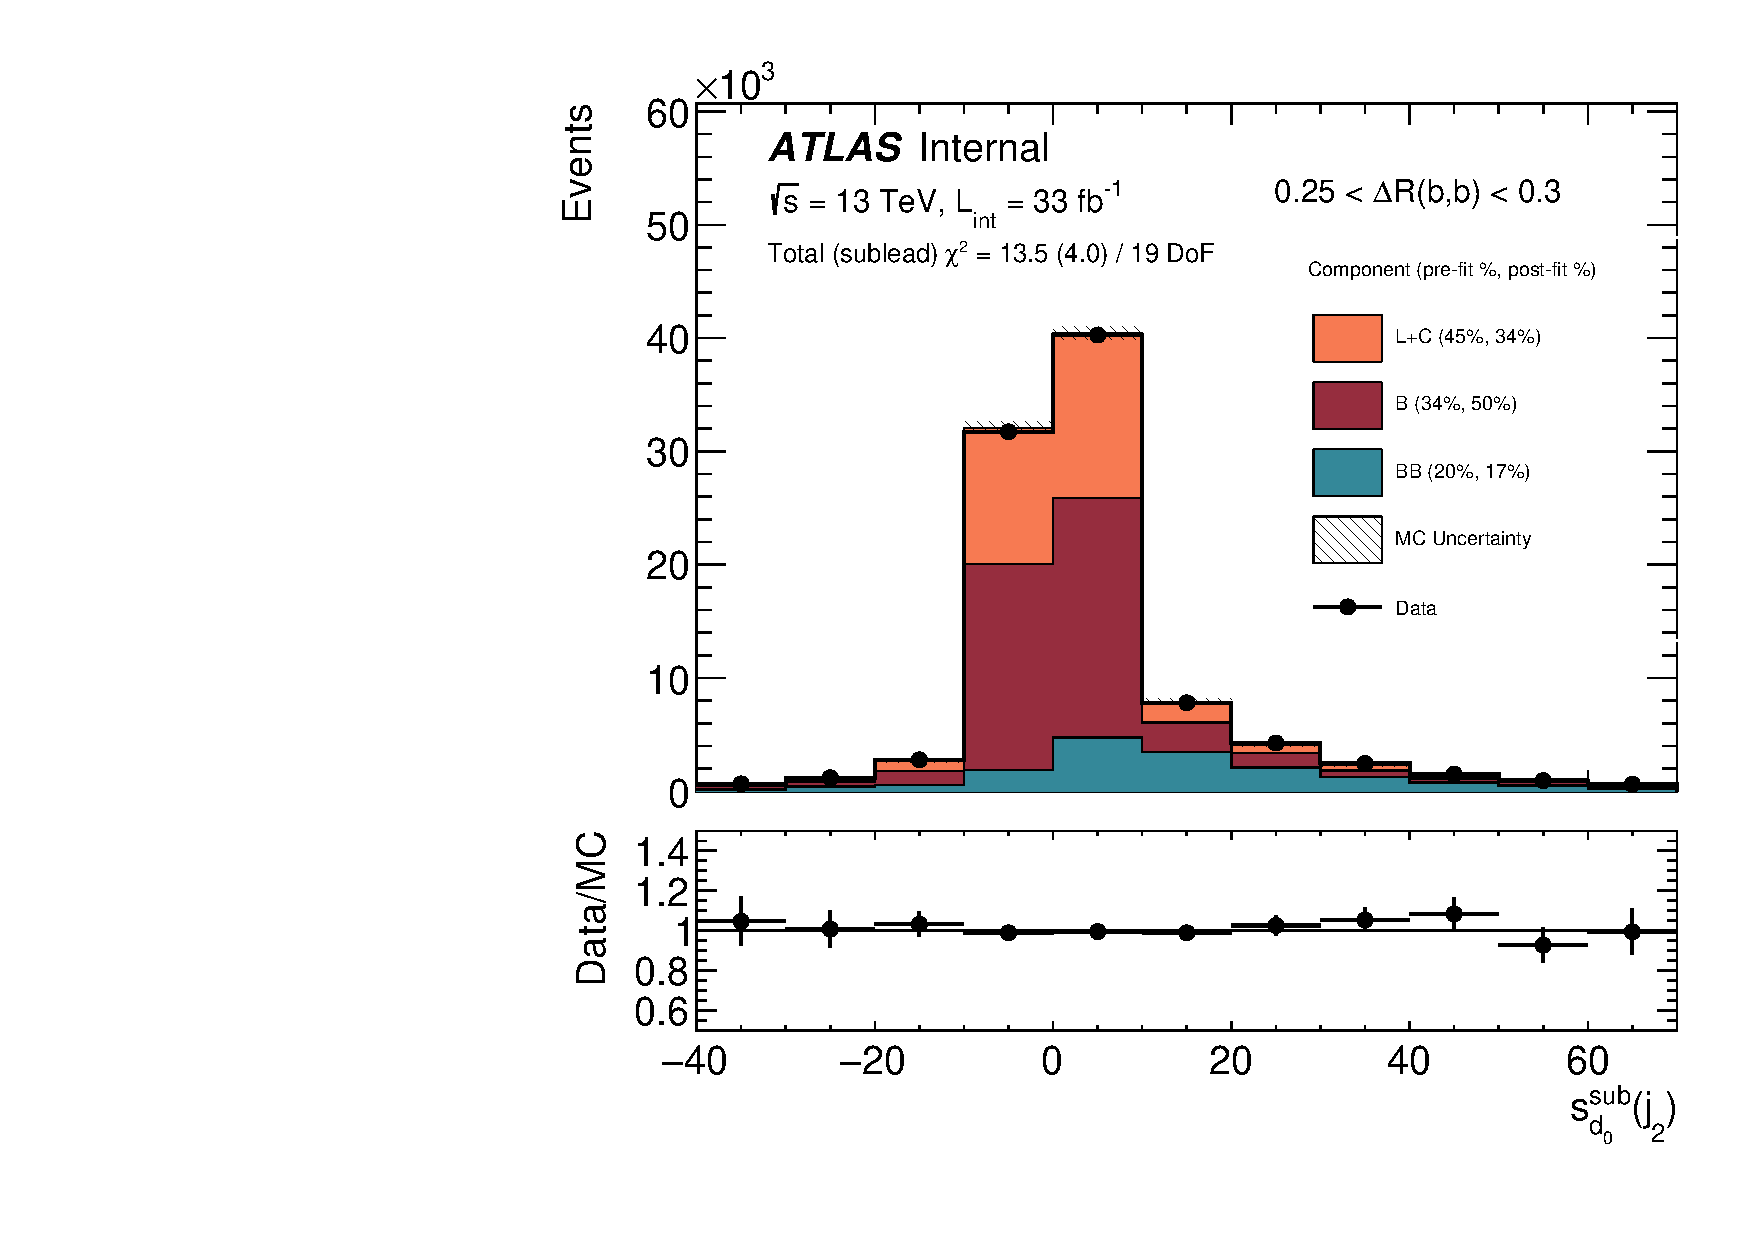
\includegraphics[width=0.45\textwidth]{figures/gbb/paperplots/Canv_Fit_b0_25_DeltaR_0_3_LpT_INF_SpT_INF_coarse_y}
 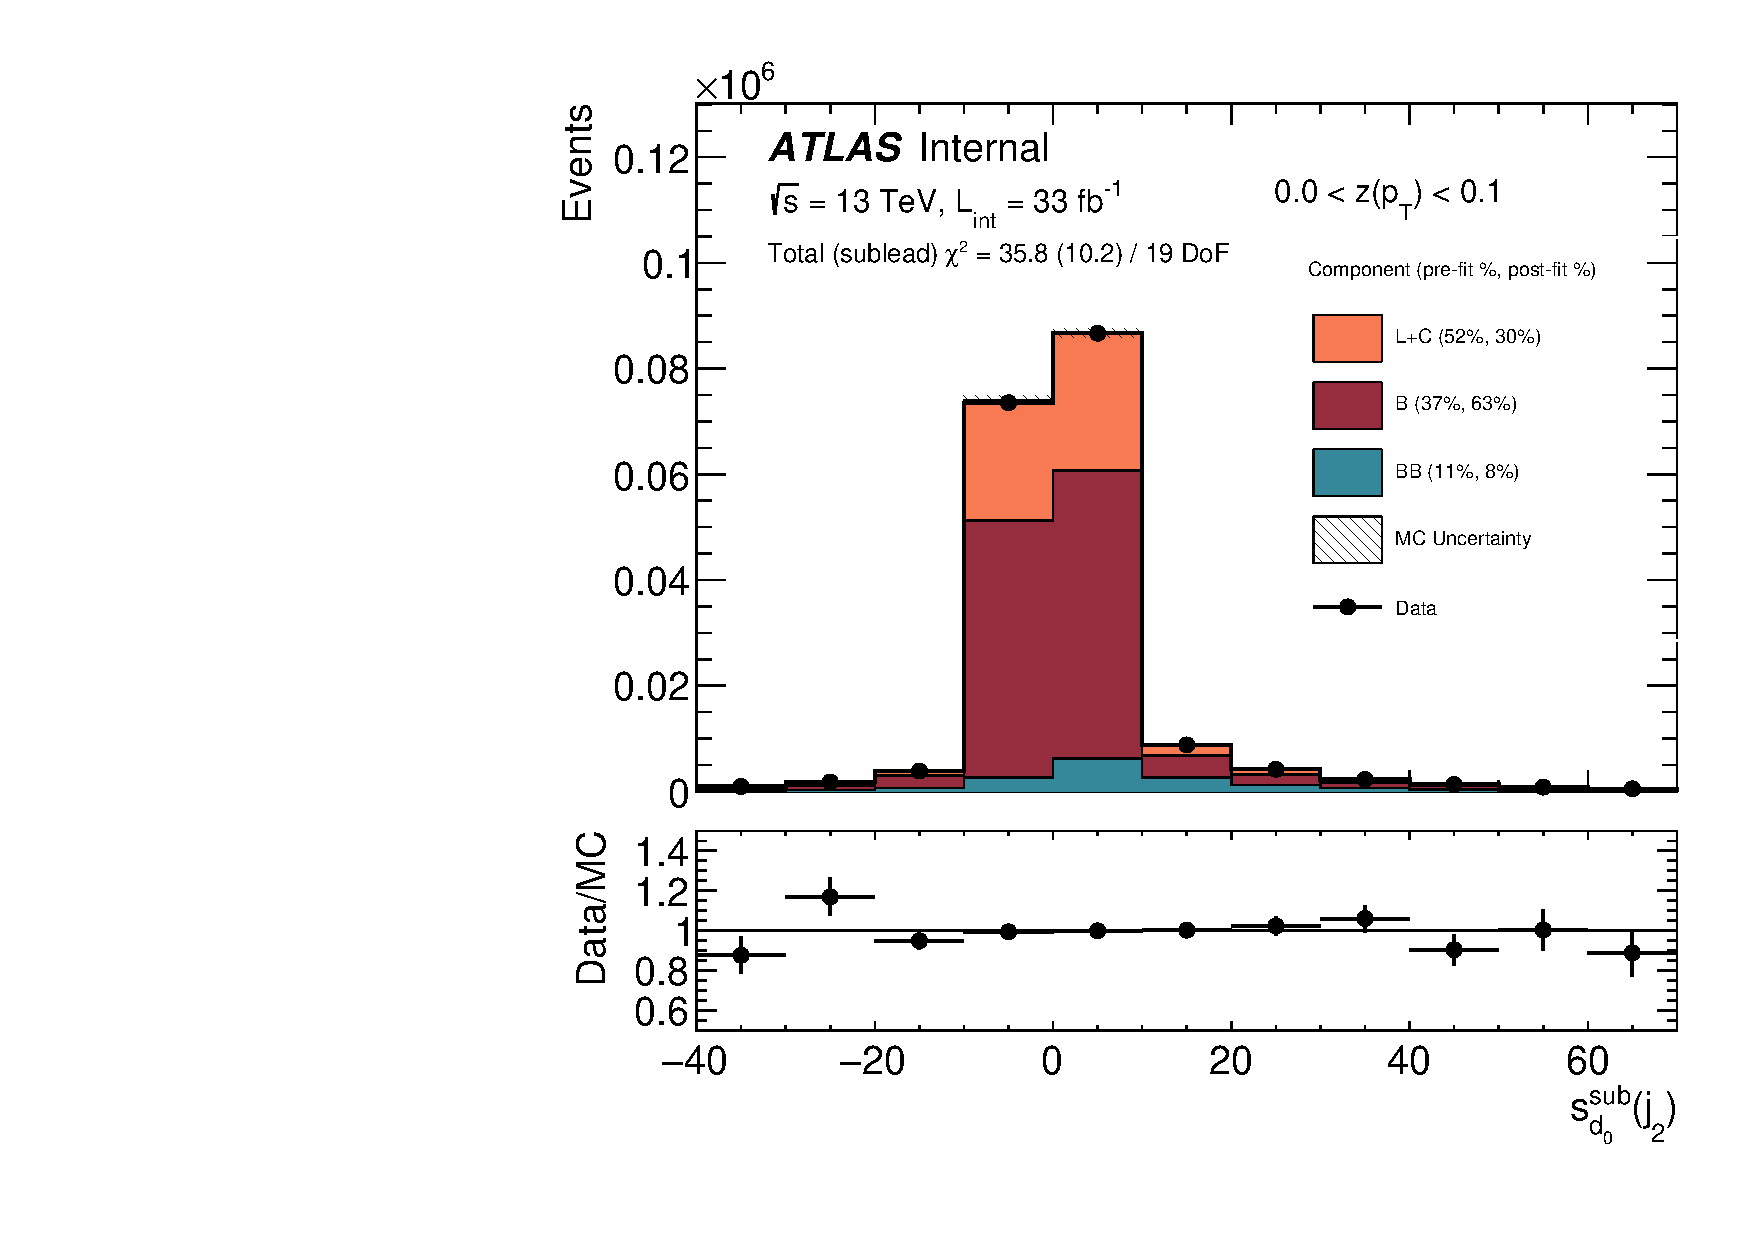
\includegraphics[width=0.45\textwidth]{figures/gbb/paperplots/Canv_Fit_b0_25_zpt_0_3_LpT_INF_SpT_INF_coarse_y}
 \includegraphics[width=0.45\textwidth]{figures/gbb/paperplots/Canv_Fit_b0_25_M_0_3_LpT_INF_SpT_INF_coarse_y}
 \includegraphics[width=0.45\textwidth]{figures/gbb/paperplots/Canv_Fit_b0_25_dphi_0_3_LpT_INF_SpT_INF_coarse_y}
\caption{Example of post-fit \subsdzero distributions of the sub-leading track jets in bin of \drbb (top left), \zpt (top right), \mpt (bottom left) and \dphi (bottom right). Error bars only include statistical uncertainties.}
  \label{fig:fit-example-subleading}
\end{figure}


\begin{figure}[htbp]
  \centering
  \includegraphics[width=0.45\textwidth]{figures/gbb/paperplots/Canv_dR_FracDataMC}
  \includegraphics[width=0.45\textwidth]{figures/gbb/paperplots/Canv_ZpT_FracDataMC}
  \includegraphics[width=0.45\textwidth]{figures/gbb/paperplots/Canv_fracmasspt_FracDataMC}       
  \includegraphics[width=0.45\textwidth]{figures/gbb/paperplots/Canv_dphi_FracDataMC}       
\caption{MC predicted (hollow) and fitted (solid) flavor fraction in bins of \drbb (top left), \zpt (top right), \mpt (bottom left) and \dphi (bottom right). The error bar is the quadrature sum of the uncertainty derived from fit range systematics and fit statistics as defined in Sec.\ref{sec:gbb-sub_systematics} }
  \label{fig:gbb-fitfrac}
\end{figure}


\begin{figure}[htbp]
  \centering
 \includegraphics[width=0.45\textwidth]{figures/gbb/Sub_Sd0_Fits/Canv_dR_leadCrossCheck.pdf}
 \includegraphics[width=0.45\textwidth]{figures/gbb/Sub_Sd0_Fits/Canv_dR_subsubCrossCheck.pdf}\\
 \includegraphics[width=0.45\textwidth]{figures/gbb/Sub_Sd0_Fits/Canv_dR_ptbinCrossCheck.pdf}
 \includegraphics[width=0.45\textwidth]{figures/gbb/Sub_Sd0_Fits/Canv_dR_noreweightCrossCheck.pdf}\\
\caption{Comparison of flavor fractions fitted (1) using \subsdzero and \sdzero (top left), (2) using \subsdzero and \subsubsdzero (top right), (3) using inclusive and $p_T$ parameterized templates (bottom left) and (4) with and without track jet kinematic re-weighting in bins of \drbb}
  \label{fig:dR-fitfrac-crosscheck}
\end{figure}

\begin{figure}[htbp]
  \centering
 \includegraphics[width=0.45\textwidth]{figures/gbb/Sub_Sd0_Fits/Canv_ZpT_leadCrossCheck.pdf}
 \includegraphics[width=0.45\textwidth]{figures/gbb/Sub_Sd0_Fits/Canv_ZpT_subsubCrossCheck.pdf}\\
 \includegraphics[width=0.45\textwidth]{figures/gbb/Sub_Sd0_Fits/Canv_ZpT_ptbinCrossCheck.pdf}
 \includegraphics[width=0.45\textwidth]{figures/gbb/Sub_Sd0_Fits/Canv_ZpT_noreweightCrossCheck.pdf}\\
\caption{Comparison of flavor fractions fitted (1) using \subsdzero and \sdzero (top left), (2) using \subsdzero and \subsubsdzero (top right), (3) using inclusive and $p_T$ parameterized templates (bottom left) and (4) with and without track jet kinematic re-weighting (bottom right) in bins of \zpt}
  \label{fig:ZpT-fitfrac-crosscheck}
\end{figure}


\begin{figure}[htbp]
  \centering
 \includegraphics[width=0.45\textwidth]{figures/gbb/Sub_Sd0_Fits/Canv_fracmasspt_leadCrossCheck.pdf}
 \includegraphics[width=0.45\textwidth]{figures/gbb/Sub_Sd0_Fits/Canv_fracmasspt_subsubCrossCheck.pdf}\\
 \includegraphics[width=0.45\textwidth]{figures/gbb/Sub_Sd0_Fits/Canv_fracmasspt_ptbinCrossCheck.pdf}
 \includegraphics[width=0.45\textwidth]{figures/gbb/Sub_Sd0_Fits/Canv_fracmasspt_noreweightCrossCheck.pdf}\\
\caption{Comparison of flavor fractions fitted (1) using \subsdzero and \sdzero (top left), (2) using \subsdzero and \subsubsdzero (top right), (3) using inclusive and $p_T$ parameterized templates (bottom left) and (4) with and without track jet kinematic re-weighting (bottom right) in bins of \mpt}
  \label{fig:fracmasspt-fitfrac-crosscheck}
\end{figure}

\begin{figure}[htbp]
  \centering
 \includegraphics[width=0.45\textwidth]{figures/gbb/Sub_Sd0_Fits/Canv_dphi_leadCrossCheck.pdf}
 \includegraphics[width=0.45\textwidth]{figures/gbb/Sub_Sd0_Fits/Canv_dphi_subsubCrossCheck.pdf}\\
 \includegraphics[width=0.45\textwidth]{figures/gbb/Sub_Sd0_Fits/Canv_dphi_ptbinCrossCheck.pdf}
 \includegraphics[width=0.45\textwidth]{figures/gbb/Sub_Sd0_Fits/Canv_dphi_noreweightCrossCheck.pdf}\\
\caption{Comparison of flavor fractions fitted (1) using \subsdzero and \sdzero (top left), (2) using \subsdzero and \subsubsdzero (top right), (3) using inclusive and $p_T$ parameterized templates (bottom left) and (4) with and without track jet kinematic re-weighting (bottom right) in bins of \dphi}
  \label{fig:dphi-fitfrac-crosscheck}
\end{figure}


\clearpage



\clearpage

%-------------------------------------------------------------------------------
\section{Unfolding procedure}
\label{sec:unfold}
%-------------------------------------------------------------------------------
\subsection{Background information}
\label{sec:gbb-unfoldingintro}

We unfold data to the space jet level phase space as defined in reco-level, i.e. same requirements of jet kinematics and multiplicity. To unfold the data, we need to correct the detector response for the reconstructed distribution, which is measured by our detector. As such distribution is usually summarized by histograms, without loss of generality, we denote it as $y_i$. We also assume at this stage the reconstructed distribution has the background subtracted. For the true distribution we are interested in, let us denote it as $x_i$, its transformation into the reconstructed distribution should be represented as: $T_{ij}e_ix_i = y_j (1-f_j)$, where $e_i$ is the efficiency factor, $f_j$ is the fake rate and $T_ij$ is the response matrix. The efficiency factor accounts for the efficiency loss of a true particle ending up outside the reco-level fiducial region. The fake factor corrects for the effect of reconstructed events originating from outside the targeted truth level fiducial region. The response matrix can be thought as a bin transition matrix between reco and truth-level quantities both of which within their proper fiducial region.

The estimation of efficiency factor and fake rates is relatively simple as they are vectors which we directly take them from MC. The estimation of $U_{ij}=T_{ij}^{-1}$, i.e. the unfolding matrix, is difficult as it involves matrix inversion which is subject to instability and large uncertainties arising from potential degeneracy. Instead, we take a Bayesian approach invented by ~\cite{D'Agostini:1994zf}, to directly estimate the unfolding matrix itself. In the language of probability and by Bayes rule, we know that

\begin{equation}
  U_{ij} = \mathrm{P}(x_i|y_j) = \frac{\mathrm{P}(y_j|x_i)\mathrm{P}(x_i)}{\sum_i \mathrm{P}(y_j|x_i)\cdot \mathrm{P}(x_i)}
  \label{eqn:unfolding:final}
\end{equation}

where $x_i$ and $y_j$ are efficiency and fake corrected true and reconstructed distributions, and $\mathrm{P}(y_j|x_i)$ are the response matrix entries. The data truth priors $\mathrm{P}(x_i)$, are not known to us but can be approximated by the MC truth distributions to start with. Through iterative procedure and using the output unfolded distribution as the next step prior, one can lower the bias once the result has converged. For this analysis the package that executes the Bayesian iterative unfolding is \texttt{RooUnfold} 1.1.1~\cite{Adye:2011gm}.

The following sections describe the details of unfolding with respect to the $g\rightarrow b\bar{b}$  measurement. Sec.~\ref{sec:gbb-unfolding:inputquantities} contains the input quantities used for unfolding: the unfolding matrices and the fake and inefficiency factors. The systematic uncertainties related to the unfolding procedure are described in Sec.~\ref{sec:gbb-systs:unfolding}. Technical closure and unfolding iteration optimization are documented in Sec.~\ref{app:gbb-unfolding:technicalclosure} and Sec.~\ref{app:gbb-unfolding:optimization} respectively.  


\subsection{Response matrices and acceptance factors}
\label{sec:gbb-unfolding:inputquantities}

The fake and efficiency factors are shown in Fig.~\ref{fig:gbb-acceptance} and Fig.~\ref{fig:gbb-fake}, respectively.  As expected, the factors are largely independent of the variables; there is a small decrease at low values in Fig.~\ref{fig:gbb-fake} in cases where the second sub-jet is lost/merged.  The unfolding matrices are shown in Fig.~\ref{fig:gbb-responsematrix1}; as the track-jet angular and momentum resolutions are superb, the matrices are very diagonal especially for angular variables.

\begin{figure}[htpb!]
\begin{center}
  \includegraphics[width=0.23\linewidth]{figures/gbb/Unfolding/dR_effic_factor.pdf}
  \includegraphics[width=0.23\linewidth]{figures/gbb/Unfolding/dphi_effic_factor.pdf}
  \includegraphics[width=0.23\linewidth]{figures/gbb/Unfolding/ZpT_effic_factor.pdf}
  \includegraphics[width=0.23\linewidth]{figures/gbb/Unfolding/fracmasspt_effic_factor.pdf}
\caption[]{The efficiency factors as described in Sec.~\ref{sec:gbb-unfoldingintro}.} 
\label{fig:gbb-acceptance}
\end{center}
\end{figure}

\begin{figure}[htpb!]
\begin{center}
  \includegraphics[width=0.23\linewidth]{figures/gbb/Unfolding/dR_fake_factor.pdf}
  \includegraphics[width=0.23\linewidth]{figures/gbb/Unfolding/dphi_fake_factor.pdf}
  \includegraphics[width=0.23\linewidth]{figures/gbb/Unfolding/ZpT_fake_factor.pdf}
  \includegraphics[width=0.23\linewidth]{figures/gbb/Unfolding/fracmasspt_fake_factor.pdf}
\caption[]{The fake factors as described in Sec.~\ref{sec:gbb-unfoldingintro}.} 
\label{fig:gbb-fake}
\end{center}
\end{figure}

\begin{figure}[htpb!]
\begin{center}
  \includegraphics[width=0.4\linewidth]{figures/gbb/Unfolding/dR_ResponseMatrix_x.pdf}
  \includegraphics[width=0.4\linewidth]{figures/gbb/Unfolding/dphi_ResponseMatrix_x.pdf}
  \includegraphics[width=0.4\linewidth]{figures/gbb/Unfolding/ZpT_ResponseMatrix_x.pdf}
  \includegraphics[width=0.4\linewidth]{figures/gbb/Unfolding/fracmasspt_ResponseMatrix_x.pdf}
\caption[]{The unfolding matrices.  } 
\label{fig:gbb-responsematrix1}
\end{center}
\end{figure}

\clearpage



\clearpage

\section{Systematic Uncertainties}
\label{sec:systs}
%-------------------------------------------------------------------------------
\subsection{Monte Carlo Statistical Uncertainties}
\label{sec:gbb-systs:MCstat}

The MC stats uncertainties are evaluated by re-sampling the response matrices from the nominal response matrix with associated MC stats uncertainty. In order to properly include correlations, the fake and inefficiency factors are set to unity (i.e. only events which pass both the detector-level and particle-level event selections are considered).

\subsection{Experimental Systematic Uncertainties}
\label{sec:gbb-systs:exp}

\begin{enumerate}
\item \textbf{R=1.0 jet JES and JER:} JES and JER uncertainty definitions can be found in Sec.\ref{sec:vbf-uncertainties}
    
%The uncertainty breakdown is shown in Fig.~\ref{fig:syst_overview_deltaR3}.
%\begin{figure}[htpb!]
%\begin{center}
%\includegraphics[width=0.45\linewidth]{figures/gbb/Unfolding/dR4_uncert_summary.pdf}\includegraphics[width=0.45\linewidth]{figures/gbb/Unfolding/dphi4_uncert_summary.pdf}\\
%\includegraphics[width=0.45\linewidth]{figures/gbb/Unfolding/ZpT4_uncert_summary.pdf}\includegraphics[width=0.45\linewidth]{figures/gbb/Unfolding/fracmasspt4_uncert_summary.pdf}
%\caption[]{A summary of the jet energy systematic uncertainties for all four observables. } 
%\label{fig:syst_overview_deltaR3}
%\end{center}
%\end{figure}

  \item \textbf{$b$-tagging scale factors:} \btagging uncertainty definitions can be found in Sec.\ref{sec:vbf-uncertainties}
  
%\begin{figure}[htpb!]
%\begin{center}
%\includegraphics[width=0.45\linewidth]{figures/gbb/Unfolding/dR3_uncert_summary.pdf}\includegraphics[width=0.45\linewidth]{figures/gbb/Unfolding/dphi3_uncert_summary.pdf}\\
%\includegraphics[width=0.45\linewidth]{figures/gbb/Unfolding/ZpT3_uncert_summary.pdf}\includegraphics[width=0.45\linewidth]{figures/gbb/Unfolding/fracmasspt3_uncert_summary.pdf}
%\caption[]{A summary of the $b$-tagging systematic uncertainties for all four observables. } 
%\label{fig:syst_overview_deltaR3b}
%\end{center}
%\end{figure}
  
  \item \textbf{Tracking:} There are five sources : inclusive efficiency, tracking in dense environment modeling uncertainties, fake rate, sagitta bias, and $d_0$ bias/resolution. The inclusive efficiency uncertainty is due to the material uncertainty.  The total uncertainty is 0.5\% for $|\eta| < 0.1$ and grows to 2.7\% by $2.3 < |\eta| < 2.5$.  The uncertainty on the tracking efficiency inside dense environments is due to the modeling of pixel cluster merging applied to tracks with $\Delta R < 0.1$~\cite{Aaboud:2017all,ATL-PHYS-PUB-2016-007,ATL-PHYS-PUB-2017-016}. Fake tracks arise from random combinatorics of hits. A 27\% uncertainty is applied to the fake rate. The sagitta bias stem from weak modes and can bias the track \pt. %The uncertainty breakdown is shown in Fig.~\ref{fig:syst_overview_deltaR1}.  
  
%    \begin{figure}[htpb!]
%\begin{center}
%\includegraphics[width=0.45\linewidth]{figures/gbb/Unfolding/dR1_uncert_summary.pdf}\includegraphics[width=0.45\linewidth]{figures/gbb/Unfolding/dphi1_uncert_summary.pdf}\\
%\includegraphics[width=0.45\linewidth]{figures/gbb/Unfolding/ZpT1_uncert_summary.pdf}\includegraphics[width=0.45\linewidth]{figures/gbb/Unfolding/fracmasspt1_uncert_summary.pdf}
%\caption[]{A summary of the tracking systematic uncertainties for all four observables. } 
%\label{fig:syst_overview_deltaR1}
%\end{center}
%\end{figure}
  
\end{enumerate}

\subsection{Background Subtraction Uncertainty}
\label{sec:gbb-systs:background}

See Sec.~\ref{sec:gbb-sub_systematics} for definitions. These are treated as fully correlated with the corresponding sources described elsewhere in this section.%The uncertainty breakdown is shown in Fig.~\ref{fig:syst_overview_deltaR2}.
  
%  \begin{figure}[htpb!]
%\begin{center}
%\includegraphics[width=0.45\linewidth]{figures/gbb/Unfolding/dR2_uncert_summary.pdf}\includegraphics[width=0.45\linewidth]{figures/gbb/Unfolding/dphi2_uncert_summary.pdf}\\
%\includegraphics[width=0.45\linewidth]{figures/gbb/Unfolding/ZpT2_uncert_summary.pdf}\includegraphics[width=0.45\linewidth]{figures/gbb/Unfolding/fracmasspt2_uncert_summary.pdf}
%\caption[]{A summary of the jet energy systematic uncertainties for all four observables. } 
%\label{fig:syst_overview_deltaR2}
%\end{center}
%\end{figure}

\subsection{Theoretical Systematic Uncertainties}
\label{sec:gbb-systs:theory}

The theoretical systematic uncertainty is taken two-fold. The prior difference between Sherpa and Pythia are taken care of in Sec.~\ref{sec:gbb-systs:unfolding}. The efficiency, fake factor and unfolding matrices difference summed in quadrature are taken to be the theoretical systematic uncertainty. It is noteworthy the agreement between data and Sherpa is closer or at least similar to that between data and Pythia for all unfolded distributions. But we do not use it as our nominal sample since statistics of Sherpa sample is two to eight times lower than that of Pythia.

%The unfolded result can depend on the modeling of jet fragmentation through the prior, the response matrix, and the correction factors.  Variations in the prior are already accounted for in the data-driven non-closure uncertainty from Sec.~\ref{sec:gbb-systs:unfolding}.  However, it is useful to examine the predictions from a different MC.  The particle-level distributions for Pythia and Sherpa are shown in Fig.~\ref{fig:frag1}.  There are significant differences between these models, especially for $\Delta\phi$ and the mass and to a lesser extent $\Delta R$ and $z$.  A comparison of the detector-level distributions, also with data appear in Fig.~\ref{fig:frag2}.   Sherpa provides a better description of the data; it is not used as baseline because the MC stats are lower.  The actual uncertainty associated to the jet fragmentation modeling is shown in Fig.~\ref{fig:syst_overview_deltaR2frag}.  The blue solid line compares Pythia with Sherpa with significant double-counting with the non-closure uncertainty.  The fake- (efficiency-)factor line uses Pythia with the fake- (efficiency-)factor replaced by the one from Sherpa.  Finally, the response matrix only line uses the Pythia response matrix, but re-weighted so that the particle-level projection is the Sherpa particle-level distribution.  The fragmentation modeling uncertainty is the sum in quadrature of these last three components.  Figure~\ref{fig:resultsvalidation3} compares the Pythia and Sherpa response matrices and shows that the truth-level re-weighting that makes the prior change does not change the response matrix (as desired).  The biggest source of uncertainty for the $\Delta\phi$ observable is from the response matrix in the first and last bins. This is because Pythia and Sherpa predict a different distribution for the leading and sub-leading track jets and thus the number of times that the angle is off by $\pi$ is different between the two.

%\textbf{Why doesn't Pythia have the same normalization as data?  }

%We compare Sherpa unfolded with Pythia with Sherpa truth.  There is some double-counting with the data-driven non-closure (Sec.~\ref{sec:gbb-systs:unfolding}).  The uncertainty breakdown is shown in Fig.~\ref{fig:syst_overview_deltaR2frag}.  

%\begin{figure}[htpb!]
%\begin{center}
%\includegraphics[width=0.45\linewidth]{figures/gbb/Unfolding/PythiavsSherpaTruthZpT.pdf}\includegraphics[width=0.45\linewidth]{figures/gbb/Unfolding/PythiavsSherpaTruthdR.pdf}\\
%\includegraphics[width=0.45\linewidth]{figures/gbb/Unfolding/PythiavsSherpaTruthdphi.pdf}\includegraphics[width=0.45\linewidth]{figures/gbb/Unfolding/PythiavsSherpaTruthfracmasspt.pdf}
%\caption[]{A particle-level comparison between Pythia and Sherpa, where Sherpa is normalized to Pythia.} 
%\label{fig:frag1}
%\end{center}
%\end{figure}
%
%\begin{figure}[htpb!]
%\begin{center}
%\includegraphics[width=0.45\linewidth]{figures/gbb/Unfolding/PythiavsSherpavsDataZpT.pdf}\includegraphics[width=0.45\linewidth]{figures/gbb/Unfolding/PythiavsSherpavsDatadR.pdf}\\
%\includegraphics[width=0.45\linewidth]{figures/gbb/Unfolding/PythiavsSherpavsDatadphi.pdf}\includegraphics[width=0.45\linewidth]{figures/gbb/Unfolding/PythiavsSherpavsDatafracmasspt.pdf}
%\caption[]{A detector-level comparison between Pythia, Sherpa, and data.  The MC is normalized to the data.} 
%\label{fig:frag2}
%\end{center}
%\end{figure}
%  
%  \begin{figure}[htpb!]
%\begin{center}
%\includegraphics[width=0.45\linewidth]{figures/gbb/Unfolding/ZpT0_uncert_summary.pdf}\includegraphics[width=0.45\linewidth]{figures/gbb/Unfolding/dR0_uncert_summary.pdf}\\
%\includegraphics[width=0.45\linewidth]{figures/gbb/Unfolding/dphi0_uncert_summary.pdf}\includegraphics[width=0.45\linewidth]{figures/gbb/Unfolding/fracmasspt0_uncert_summary.pdf}
%\caption[]{A summary of the fragmentation modeling uncertainty for all four observables.  The blue solid line compares Pythia with Sherpa with significant double-counting with the non-closure uncertainty.  The fake- (efficiency-)factor line uses Pythia with the fake- (efficiency-)factor replaced by the one from Sherpa.  Finally, the response matrix only line uses the Pythia response matrix, but re-weighted so that the particle-level projection is the Sherpa particle-level distribution.  The fragmentation modeling uncertainty is the sum in quadrature of these last three components. } 
%\label{fig:syst_overview_deltaR2frag}
%\end{center}
%\end{figure}
%
%\begin{figure}[htpb!]
%\begin{center}
%\includegraphics[width=0.3\linewidth]{figures/gbb/Unfolding/testPythiaZpT.pdf}\includegraphics[width=0.3\linewidth]{figures/gbb/Unfolding/testSherpaZpT.pdf}
%\includegraphics[width=0.3\linewidth]{figures/gbb/Unfolding/testSherpa_norwZpT.pdf}\\
%
%\includegraphics[width=0.3\linewidth]{figures/gbb/Unfolding/testPythiafracmasspt.pdf}\includegraphics[width=0.3\linewidth]{figures/gbb/Unfolding/testSherpafracmasspt.pdf}
%\includegraphics[width=0.3\linewidth]{figures/gbb/Unfolding/testSherpa_norwfracmasspt.pdf}\\
%
%\includegraphics[width=0.3\linewidth]{figures/gbb/Unfolding/testPythiadR.pdf}\includegraphics[width=0.3\linewidth]{figures/gbb/Unfolding/testSherpadR.pdf}
%\includegraphics[width=0.3\linewidth]{figures/gbb/Unfolding/testSherpa_norwdR.pdf}\\
%
%\includegraphics[width=0.3\linewidth]{figures/gbb/Unfolding/testPythiadphi.pdf}\includegraphics[width=0.3\linewidth]{figures/gbb/Unfolding/testSherpadphi.pdf}
%\includegraphics[width=0.3\linewidth]{figures/gbb/Unfolding/testSherpa_norwdphi.pdf}
%
%\caption[]{A detector-level comparison between Pythia, Sherpa, and data.  The MC is normalized to the data.} 
%\label{fig:frag2}
%\end{center}
%\end{figure}

\subsection{Unfolding Non-closure}
\label{sec:gbb-systs:unfolding}

The standard method~\cite{Armbruster:1694351} for evaluating the systematic uncertainty from the procedure is to re-weight the MC to the data and take the difference between the unfolded re-weighted reconstructed MC to the truth MC of the same generator.

%The re-weighted truth is a \textit{reasonable} prior with which we can estimate the bias from the choice of prior in the unfolding method.   Define the following histograms ($x_i$ will interchangeably mean the histogram $x$ and also the content in the $i^{th}$ bin of $x$):
%
%\begin{description}
%\item[$d_i$]: The measured spectrum. 
%\item[$R_{ij}$]: The response matrix such that $R_{ij}$ contains the number of events in the simulation that fall in the reconstructed bin $i$ and the truth bin $j$.
%\item[$t_i$]: $t_i = \sum_j R_{ji}$, i.e. the truth spectrum for events that pass both truth and reconstructed selections.
%\item[$r_i$]: $r_i = \sum_j R_{ij}$, i.e. the reconstructed spectrum for events that pass both truth and reconstructed selections
%\item[$\tilde{R}_{ij}$]: The normalized version of $R_{ij}$ such that $r_i = \sum_j \tilde{R}_{ij} t_j$.  Explicitly, $\tilde{R}_{ij} = R_{ij}/\sum_{i'} R_{i'j}$.  The entries of $\tilde{R}_{ij}$ are the conditional probability for a truth event in bin $j$ to be reconstructed in bin $i$.
%\end{description}
%
%\noindent The re-weighting procedure can only be applied to simulation events which pass both the truth and reconstructed event selections and so the first step is to take the data and apply a correction $\epsilon_i$ bin-by-bin given by 
%
%\begin{align}
%\epsilon_i = \frac{\text{Pass both reconstructed and truth selections}}{\text{Pass the reconstructed selection}},
%\end{align}
%
%\noindent where $i$ is the bin number.   Define $\tilde{d}_i = \epsilon_i d_i$ to be the corrected data histogram.  We want now a prior $\tilde{t}_i$ such that $\tilde{R}_{ij} \tilde{t}_j$ is very close to $\tilde{d}_i$.  Since $\tilde{R}_{ij}$ is not too far from a diagonal matrix, one way of generating $\tilde{t}_i$ is to use weights built from the reconstructed simulation: $w_i = \tilde{d}_i/r_i$.  Define $\tilde{t}_i=w_it_i$.  Fig. X shows that the weights $w_i$ are effective at improving the data/MC agreement of $\tilde{r}_i=\sum_j\tilde{R}_{ij}\tilde{t}_j$ with respect to $r_i$.  The non-closure uncertainty is then given by
%
%\begin{align}
%\sigma_i=\text{Unfold[nominal response matrix]}\left(\tilde{R}_{ij} \tilde{t}_j\right)-\tilde{t}_i
%\end{align}

%\textbf{In other words}, we have a function $f(d,p,R)$ which takes as inputs three histograms (data $d$, prior $p$, and the response matrix $R$) and outputs another histogram (the unfolding function).  By construction, $p=f(Rp,p,R)$ (not being careful about the normalization of $p$ and $R$, as above).  We pick $t$ such that $Rt\sim d$.  Then, the non-closure uncertainty is the difference between $f(Rt,p,R)$ and $t$.  The use of the word 'prior' is slightly misleading, since $p$ is still the prior used in the unfolding.

%Figure~\ref{fig:nonclosure1} shows the re-weighting factors and Fig.~\ref{fig:nonclosure2} shows that they work well, as expected since the response matrices are so diagonal.  The actual non-closure uncertainty is quite small and much smaller than the raw data/MC difference (Fig.~\ref{fig:nonclosure3}).
%
%\begin{figure}[htpb!]
%\begin{center}
%\includegraphics[width=0.45\linewidth]{figures/gbb/Unfolding/noc_factors_dR.pdf}\includegraphics[width=0.45\linewidth]{figures/gbb/Unfolding/noc_factors_dphi.pdf}\\
%\includegraphics[width=0.45\linewidth]{figures/gbb/Unfolding/noc_factors_ZpT.pdf}\includegraphics[width=0.45\linewidth]{figures/gbb/Unfolding/noc_factors_fracmasspt.pdf}
%\caption[]{The correction factors applied for the data-driven non-closure uncertainty. } 
%\label{fig:nonclosure1}
%\end{center}
%\end{figure}
%
%\begin{figure}[htpb!]
%\begin{center}
%\includegraphics[width=0.45\linewidth]{figures/gbb/Unfolding/noc_datamc_dR.pdf}\includegraphics[width=0.45\linewidth]{figures/gbb/Unfolding/noc_datamc_dphi.pdf}\\
%\includegraphics[width=0.45\linewidth]{figures/gbb/Unfolding/noc_datamc_ZpT.pdf}\includegraphics[width=0.45\linewidth]{figures/gbb/Unfolding/noc_datamc_fracmasspt.pdf}
%\caption[]{A comparison of the data/MC difference before and after the re-weighting is applied. } 
%\label{fig:nonclosure2}
%\end{center}
%\end{figure}
%
%\begin{figure}[htpb!]
%\begin{center}
%\includegraphics[width=0.45\linewidth]{figures/gbb/Unfolding/non_uncertainty_mean_dR.pdf}\includegraphics[width=0.45\linewidth]{figures/gbb/Unfolding/non_uncertainty_mean_dphi.pdf}\\
%\includegraphics[width=0.45\linewidth]{figures/gbb/Unfolding/non_uncertainty_mean_ZpT.pdf}\includegraphics[width=0.45\linewidth]{figures/gbb/Unfolding/non_uncertainty_mean_fracmasspt.pdf}
%\caption[]{A comparison of the non-closure uncertainty with the raw data/MC difference. } 
%\label{fig:nonclosure3}
%\end{center}
%\end{figure}



\subsection{Summary}
\label{sec:gbb-systs:overview}

Figure~\ref{fig:syst_overview_deltaR} presents a summary of the unfolded distribution systematic uncertainties. The largest source of uncertainty is theoretical uncertainty. Background subtraction uncertainties and detector uncertainties are the next ones in rank.

\begin{figure}[htpb!]
\begin{center}
\includegraphics[width=0.45\linewidth]{figures/gbb/Unfolding/dR_uncert_summary.pdf}\includegraphics[width=0.45\linewidth]{figures/gbb/Unfolding/dphi_uncert_summary.pdf}\\
\includegraphics[width=0.45\linewidth]{figures/gbb/Unfolding/ZpT_uncert_summary.pdf}\includegraphics[width=0.45\linewidth]{figures/gbb/Unfolding/fracmasspt_uncert_summary.pdf}
\caption[]{A summary of the systematic uncertainties for all four observables. } 
\label{fig:syst_overview_deltaR}
\end{center}
\end{figure}



\clearpage

%-------------------------------------------------------------------------------
\section{Results}
\label{sec:results}
%-------------------------------------------------------------------------------

Figure~\ref{fig:results} presents a summary of the results.

\begin{figure}[htpb!]
\begin{center}
\includegraphics[width=0.45\linewidth]{figures/Unfolding/dR_unfolded_data.pdf}\includegraphics[width=0.45\linewidth]{figures/Unfolding/dphi_unfolded_data.pdf}\\
\includegraphics[width=0.45\linewidth]{figures/Unfolding/ZpT_unfolded_data.pdf}\includegraphics[width=0.45\linewidth]{figures/Unfolding/fracmasspt_unfolded_data.pdf}
\caption[]{The unfolded data compared with Pythia. The data points have error bars that are the statistical uncertainties and the bands are the total systematic uncertainties described in Sec.~\ref{sec:systs}.} 
\label{fig:results}
\end{center}
\end{figure}

\section{Interpretation}
\label{sec:interp}

The data will be made available through HepData so MC authors will be able to compare their models with our data at a later time.  However, it is interesting to provide some comparisons in the ATLAS paper.  Due to the large MC sizes needed for this study, we have privately produced a series of samples discussed in this section.  This setup has been extensively validated, as discussed in Appendix~\ref{sec:app-truthpreds}.  

% All figures and tables should appear before the summary and conclusion.
% The package placeins provides the macro \FloatBarrier to achieve this.
\FloatBarrier


%-------------------------------------------------------------------------------
\section{Conclusion}
\label{sec:conclusion}
%-------------------------------------------------------------------------------

We have performed a measurement of $g\rightarrow b\bar{b}$ in the small opening angle regime; the first such measurement with multiple bins below $\Delta R= 0.4$.  Key observables related to the gluon and $b\bar{b}$ kinematics are unfolded to particle-level and compared with MC generators formally at leading logarithm accuracy.  The overall agreement between the simulation and the data is excellent, with some indication of mis-modeling in low $\Delta R$ (low $z$, low mass) regimes.  Interestingly, the $b\bar{b}$ opening angle with respect to the gluon production plane seems to indicate less polarization than predicted by Pythia 8.  This puzzle and the results in general are important inputs for the MC community and will hopefully help to improve our understanding of massive splitting in QCD as well as an important background for many high $p_\text{T}$ searches and measurements with Higgs bosons.


%% %-------------------------------------------------------------------------------
%% \section*{Acknowledgements}
%% %-------------------------------------------------------------------------------

%% %% Acknowledgements for papers with collision data
% Version 14-Feb-2018

% Standard acknowledgements start here
%----------------------------------------------
We thank CERN for the very successful operation of the LHC, as well as the
support staff from our institutions without whom ATLAS could not be
operated efficiently.

We acknowledge the support of ANPCyT, Argentina; YerPhI, Armenia; ARC, Australia; BMWFW and FWF, Austria; ANAS, Azerbaijan; SSTC, Belarus; CNPq and FAPESP, Brazil; NSERC, NRC and CFI, Canada; CERN; CONICYT, Chile; CAS, MOST and NSFC, China; COLCIENCIAS, Colombia; MSMT CR, MPO CR and VSC CR, Czech Republic; DNRF and DNSRC, Denmark; IN2P3-CNRS, CEA-DRF/IRFU, France; SRNSFG, Georgia; BMBF, HGF, and MPG, Germany; GSRT, Greece; RGC, Hong Kong SAR, China; ISF, I-CORE and Benoziyo Center, Israel; INFN, Italy; MEXT and JSPS, Japan; CNRST, Morocco; NWO, Netherlands; RCN, Norway; MNiSW and NCN, Poland; FCT, Portugal; MNE/IFA, Romania; MES of Russia and NRC KI, Russian Federation; JINR; MESTD, Serbia; MSSR, Slovakia; ARRS and MIZ\v{S}, Slovenia; DST/NRF, South Africa; MINECO, Spain; SRC and Wallenberg Foundation, Sweden; SERI, SNSF and Cantons of Bern and Geneva, Switzerland; MOST, Taiwan; TAEK, Turkey; STFC, United Kingdom; DOE and NSF, United States of America. In addition, individual groups and members have received support from BCKDF, the Canada Council, CANARIE, CRC, Compute Canada, FQRNT, and the Ontario Innovation Trust, Canada; EPLANET, ERC, ERDF, FP7, Horizon 2020 and Marie Sk{\l}odowska-Curie Actions, European Union; Investissements d'Avenir Labex and Idex, ANR, R{\'e}gion Auvergne and Fondation Partager le Savoir, France; DFG and AvH Foundation, Germany; Herakleitos, Thales and Aristeia programmes co-financed by EU-ESF and the Greek NSRF; BSF, GIF and Minerva, Israel; BRF, Norway; CERCA Programme Generalitat de Catalunya, Generalitat Valenciana, Spain; the Royal Society and Leverhulme Trust, United Kingdom.

The crucial computing support from all WLCG partners is acknowledged gratefully, in particular from CERN, the ATLAS Tier-1 facilities at TRIUMF (Canada), NDGF (Denmark, Norway, Sweden), CC-IN2P3 (France), KIT/GridKA (Germany), INFN-CNAF (Italy), NL-T1 (Netherlands), PIC (Spain), ASGC (Taiwan), RAL (UK) and BNL (USA), the Tier-2 facilities worldwide and large non-WLCG resource providers. Major contributors of computing resources are listed in Ref.~\cite{ATL-GEN-PUB-2016-002}.
%----------------------------------------------



%% The \texttt{atlaslatex} package contains the acknowledgements that were valid 
%% at the time of the release you are using.
%% These can be found in the \texttt{acknowledgements} subdirectory.
%% When your ATLAS paper or PUB/CONF note is ready to be published,
%% download the latest set of acknowledgements from:\\
%% \url{https://twiki.cern.ch/twiki/bin/view/AtlasProtected/PubComAcknowledgements}

%% The supporting notes for the analysis should also contain a list of contributors.
%% This information should usually be included in \texttt{mydocument-metadata.tex}.
%% The list should be printed either here or before the table of contents.


%-------------------------------------------------------------------------------
\clearpage
\appendix
\part*{Appendix}
\addcontentsline{toc}{part}{Appendix}
%-------------------------------------------------------------------------------

\clearpage
\section{\subsdzero templates}
\label{sec:app-sd0templates}
%%%%%%%%%%%%%%%%%%%%%%%%%%%%%%%%%%%%

In this section we show the \subsdzero templates in bins of the observables we are measuring. 

\subsection{$\Delta R$}

The leading and sub-leading track jets template \subsdzero distributions in bins of $\Delta R$ are shown in Figures.\ref{fig:dR-template-leading},\ref{fig:dR-template-subleading}.

\begin{figure}[htbp]
  \centering
 \includegraphics[width=0.32\textwidth]{figures/Sub_Sd0_Fits/Canv_FitTemplate_02-DeltaR-025_LpT_INF_SpT_INF_x.pdf}
 \includegraphics[width=0.32\textwidth]{figures/Sub_Sd0_Fits/Canv_FitTemplate_025-DeltaR-03_LpT_INF_SpT_INF_x.pdf}
 \includegraphics[width=0.32\textwidth]{figures/Sub_Sd0_Fits/Canv_FitTemplate_03-DeltaR-04_LpT_INF_SpT_INF_x.pdf}\\
 \includegraphics[width=0.32\textwidth]{figures/Sub_Sd0_Fits/Canv_FitTemplate_04-DeltaR-05_LpT_INF_SpT_INF_x.pdf}
 \includegraphics[width=0.32\textwidth]{figures/Sub_Sd0_Fits/Canv_FitTemplate_05-DeltaR-06_LpT_INF_SpT_INF_x.pdf}
 \includegraphics[width=0.32\textwidth]{figures/Sub_Sd0_Fits/Canv_FitTemplate_06-DeltaR-07_LpT_INF_SpT_INF_x.pdf}\\

\caption{Template \subsdzero distributions of the leading track jet in bins of $\Delta R$. }
  \label{fig:dR-template-leading}
\end{figure}


\begin{figure}[htbp]
  \centering
 \includegraphics[width=0.32\textwidth]{figures/Sub_Sd0_Fits/Canv_FitTemplate_02-DeltaR-025_LpT_INF_SpT_INF_y.pdf}
 \includegraphics[width=0.32\textwidth]{figures/Sub_Sd0_Fits/Canv_FitTemplate_025-DeltaR-03_LpT_INF_SpT_INF_y.pdf}
 \includegraphics[width=0.32\textwidth]{figures/Sub_Sd0_Fits/Canv_FitTemplate_03-DeltaR-04_LpT_INF_SpT_INF_y.pdf}\\
 \includegraphics[width=0.32\textwidth]{figures/Sub_Sd0_Fits/Canv_FitTemplate_04-DeltaR-05_LpT_INF_SpT_INF_y.pdf}
 \includegraphics[width=0.32\textwidth]{figures/Sub_Sd0_Fits/Canv_FitTemplate_05-DeltaR-06_LpT_INF_SpT_INF_y.pdf}
 \includegraphics[width=0.32\textwidth]{figures/Sub_Sd0_Fits/Canv_FitTemplate_06-DeltaR-07_LpT_INF_SpT_INF_y.pdf}\\

\caption{Template \subsdzero distributions of the sub-leading track jet in bins of $\Delta R$. }
  \label{fig:dR-template-subleading}
\end{figure}


\clearpage
\subsection{\zpt}

The leading and sub-leading track jets template \subsdzero distributions in bins of \zpt are shown in Figures.\ref{fig:ZpT-template-leading},\ref{fig:ZpT-template-subleading}.

\begin{figure}[htbp]
  \centering
 \includegraphics[width=0.32\textwidth]{figures/Sub_Sd0_Fits/Canv_FitTemplate_0-Zp_T-01_LpT_INF_SpT_INF_x.pdf}
 \includegraphics[width=0.32\textwidth]{figures/Sub_Sd0_Fits/Canv_FitTemplate_01-Zp_T-02_LpT_INF_SpT_INF_x.pdf}
 \includegraphics[width=0.32\textwidth]{figures/Sub_Sd0_Fits/Canv_FitTemplate_02-Zp_T-03_LpT_INF_SpT_INF_x.pdf}\\
 \includegraphics[width=0.32\textwidth]{figures/Sub_Sd0_Fits/Canv_FitTemplate_03-Zp_T-04_LpT_INF_SpT_INF_x.pdf}
 \includegraphics[width=0.32\textwidth]{figures/Sub_Sd0_Fits/Canv_FitTemplate_04-Zp_T-05_LpT_INF_SpT_INF_x.pdf}

\caption{Template \subsdzero distributions of the leading track jet in bins of \zpt. }
  \label{fig:ZpT-template-leading}
\end{figure}


\begin{figure}[htbp]
  \centering
 \includegraphics[width=0.32\textwidth]{figures/Sub_Sd0_Fits/Canv_FitTemplate_0-Zp_T-01_LpT_INF_SpT_INF_y.pdf}
 \includegraphics[width=0.32\textwidth]{figures/Sub_Sd0_Fits/Canv_FitTemplate_01-Zp_T-02_LpT_INF_SpT_INF_y.pdf}
 \includegraphics[width=0.32\textwidth]{figures/Sub_Sd0_Fits/Canv_FitTemplate_02-Zp_T-03_LpT_INF_SpT_INF_y.pdf}\\
 \includegraphics[width=0.32\textwidth]{figures/Sub_Sd0_Fits/Canv_FitTemplate_03-Zp_T-04_LpT_INF_SpT_INF_y.pdf}
 \includegraphics[width=0.32\textwidth]{figures/Sub_Sd0_Fits/Canv_FitTemplate_04-Zp_T-05_LpT_INF_SpT_INF_y.pdf}

\caption{Template \subsdzero distributions of the sub-leading track jet in bins of \zpt. }
  \label{fig:ZpT-template-subleading}
\end{figure}



\clearpage
%\subsection{\mpt}
%
%The leading and sub-leading track jets template \subsdzero distributions in bins of \mpt are shown in Figures.\ref{fig:fracmasspt-template-leading},\ref{fig:fracmasspt-template-subleading}.
%
%\begin{figure}[htbp]
%  \centering
% \includegraphics[width=0.32\textwidth]{figures/Sub_Sd0_Fits/Canv_FitTemplate_-30-logMbbpTG--22_LpT_INF_SpT_INF_x.pdf}
% \includegraphics[width=0.32\textwidth]{figures/Sub_Sd0_Fits/Canv_FitTemplate_-22-logMbbpTG--19_LpT_INF_SpT_INF_x.pdf}
% \includegraphics[width=0.32\textwidth]{figures/Sub_Sd0_Fits/Canv_FitTemplate_-19-logMbbpTG--16_LpT_INF_SpT_INF_x.pdf}\\
% \includegraphics[width=0.32\textwidth]{figures/Sub_Sd0_Fits/Canv_FitTemplate_-16-logMbbpTG--13_LpT_INF_SpT_INF_x.pdf}
% \includegraphics[width=0.32\textwidth]{figures/Sub_Sd0_Fits/Canv_FitTemplate_-13-logMbbpTG--0_LpT_INF_SpT_INF_x.pdf}
%
%\caption{Template \subsdzero distributions of the leading track jet in bins of \mpt. }
%  \label{fig:fracmasspt-template-leading}
%\end{figure}
%
%
%\begin{figure}[htbp]
%  \centering
% \includegraphics[width=0.32\textwidth]{figures/Sub_Sd0_Fits/Canv_FitTemplate_-30-logMbbpTG--22_LpT_INF_SpT_INF_y.pdf}
% \includegraphics[width=0.32\textwidth]{figures/Sub_Sd0_Fits/Canv_FitTemplate_-22-logMbbpTG--19_LpT_INF_SpT_INF_y.pdf}
% \includegraphics[width=0.32\textwidth]{figures/Sub_Sd0_Fits/Canv_FitTemplate_-19-logMbbpTG--16_LpT_INF_SpT_INF_y.pdf}\\
% \includegraphics[width=0.32\textwidth]{figures/Sub_Sd0_Fits/Canv_FitTemplate_-16-logMbbpTG--13_LpT_INF_SpT_INF_y.pdf}
% \includegraphics[width=0.32\textwidth]{figures/Sub_Sd0_Fits/Canv_FitTemplate_-13-logMbbpTG--0_LpT_INF_SpT_INF_y.pdf}
%
%\caption{Template \subsdzero distributions of the sub-leading track jet in bins of \mpt. }
%  \label{fig:fracmasspt-template-subleading}
%\end{figure}


\clearpage
\subsection{\dphi}

The leading and sub-leading track jets template \subsdzero distributions in bins of \dphi are shown in Figures.\ref{fig:dphi-template-leading},\ref{fig:dphi-template-subleading}.

\begin{figure}[htbp]
  \centering
 \includegraphics[width=0.32\textwidth]{figures/Sub_Sd0_Fits/Canv_FitTemplate_0-Deltaphi-0628_LpT_INF_SpT_INF_x.pdf}
 \includegraphics[width=0.32\textwidth]{figures/Sub_Sd0_Fits/Canv_FitTemplate_0628-Deltaphi-1256_LpT_INF_SpT_INF_x.pdf}
 \includegraphics[width=0.32\textwidth]{figures/Sub_Sd0_Fits/Canv_FitTemplate_1256-Deltaphi-1884_LpT_INF_SpT_INF_x.pdf}\\
 \includegraphics[width=0.32\textwidth]{figures/Sub_Sd0_Fits/Canv_FitTemplate_1884-Deltaphi-2512_LpT_INF_SpT_INF_x.pdf}
 \includegraphics[width=0.32\textwidth]{figures/Sub_Sd0_Fits/Canv_FitTemplate_2512-Deltaphi-3140_LpT_INF_SpT_INF_x.pdf}

\caption{Template \subsdzero distributions of the leading track jet in bins of \dphi. }
  \label{fig:dphi-template-leading}
\end{figure}


\begin{figure}[htbp]
  \centering
 \includegraphics[width=0.32\textwidth]{figures/Sub_Sd0_Fits/Canv_FitTemplate_0-Deltaphi-0628_LpT_INF_SpT_INF_y.pdf}
 \includegraphics[width=0.32\textwidth]{figures/Sub_Sd0_Fits/Canv_FitTemplate_0628-Deltaphi-1256_LpT_INF_SpT_INF_y.pdf}
 \includegraphics[width=0.32\textwidth]{figures/Sub_Sd0_Fits/Canv_FitTemplate_1256-Deltaphi-1884_LpT_INF_SpT_INF_y.pdf}\\
 \includegraphics[width=0.32\textwidth]{figures/Sub_Sd0_Fits/Canv_FitTemplate_1884-Deltaphi-2512_LpT_INF_SpT_INF_y.pdf}
 \includegraphics[width=0.32\textwidth]{figures/Sub_Sd0_Fits/Canv_FitTemplate_2512-Deltaphi-3140_LpT_INF_SpT_INF_y.pdf}

\caption{Template \subsdzero distributions of the sub-leading track jet in bins of \dphi. }
  \label{fig:dphi-template-subleading}
\end{figure}



\clearpage
\section{Systematics effects on templates}
\label{sec:app-sysvariations}
%%%%%%%%%%%%%%%%%%%%%%%%%%%%%%%%%%%%
In this section we show the effects of systematic variations on \subsdzero templates. The flavor tagging, JES/JER, parton shower and tracking variations for leading and sub-leading track jets in events with $0.25<\Delta R<0.3$ are shown in Fig. \ref{fig:sys-lead-ftag} \ref{fig:sys-lead-jes-jer} \ref{fig:sys-lead-ps} \ref{fig:sys-lead-trk} and Fig. \ref{fig:sys-sublead-ftag} \ref{fig:sys-sublead-jes-jer} \ref{fig:sys-sublead-ps} \ref{fig:sys-sublead-trk} respectively.

\begin{figure}[htbp]
  \centering
 \includegraphics[width=0.32\textwidth]{figures/Sub_Sd0_Sys_Variations/Canv_Lead_Sub_Sd0_FTAG_Variation_BB.pdf}
 \includegraphics[width=0.32\textwidth]{figures/Sub_Sd0_Sys_Variations/Canv_Lead_Sub_Sd0_FTAG_Variation_B.pdf}
 \includegraphics[width=0.32\textwidth]{figures/Sub_Sd0_Sys_Variations/Canv_Lead_Sub_Sd0_FTAG_Variation_LC.pdf}
\caption{Template \subsdzero variations of flavor tagging systematics for the leading track jet in bin of $0.25<\Delta R<0.3$. }
  \label{fig:sys-lead-ftag}
\end{figure}

\begin{figure}[htbp]
  \centering
 \includegraphics[width=0.32\textwidth]{figures/Sub_Sd0_Sys_Variations/Canv_Lead_Sub_Sd0_JET_Variation_BB.pdf}
 \includegraphics[width=0.32\textwidth]{figures/Sub_Sd0_Sys_Variations/Canv_Lead_Sub_Sd0_JET_Variation_B.pdf}
 \includegraphics[width=0.32\textwidth]{figures/Sub_Sd0_Sys_Variations/Canv_Lead_Sub_Sd0_JET_Variation_LC.pdf}
\caption{Template \subsdzero variations of JES/JER systematics for the leading track jet in bin of $0.25<\Delta R<0.3$. }
  \label{fig:sys-lead-jes-jer}
\end{figure}

\begin{figure}[htbp]
  \centering
 \includegraphics[width=0.32\textwidth]{figures/Sub_Sd0_Sys_Variations/Canv_Lead_Sub_Sd0_PS_Variation_BB.pdf}
 \includegraphics[width=0.32\textwidth]{figures/Sub_Sd0_Sys_Variations/Canv_Lead_Sub_Sd0_PS_Variation_B.pdf}
 \includegraphics[width=0.32\textwidth]{figures/Sub_Sd0_Sys_Variations/Canv_Lead_Sub_Sd0_PS_Variation_LC.pdf}
\caption{Template \subsdzero variations of parton shower systematics for the leading track jet in bin of $0.25<\Delta R<0.3$. }
  \label{fig:sys-lead-ps}
\end{figure}


\begin{figure}[htbp]
  \centering
 \includegraphics[width=0.32\textwidth]{figures/Sub_Sd0_Sys_Variations/Canv_Lead_Sub_Sd0_TRK_Variation_BB.pdf}
 \includegraphics[width=0.32\textwidth]{figures/Sub_Sd0_Sys_Variations/Canv_Lead_Sub_Sd0_TRK_Variation_B.pdf}
 \includegraphics[width=0.32\textwidth]{figures/Sub_Sd0_Sys_Variations/Canv_Lead_Sub_Sd0_TRK_Variation_LC.pdf}
\caption{Template \subsdzero variations of tracking systematics for the leading track jet in bin of $0.25<\Delta R<0.3$. }
  \label{fig:sys-lead-trk}
\end{figure}



\begin{figure}[htbp]
  \centering
 \includegraphics[width=0.32\textwidth]{figures/Sub_Sd0_Sys_Variations/Canv_SubLead_Sub_Sd0_FTAG_Variation_BB.pdf}
 \includegraphics[width=0.32\textwidth]{figures/Sub_Sd0_Sys_Variations/Canv_SubLead_Sub_Sd0_FTAG_Variation_B.pdf}
 \includegraphics[width=0.32\textwidth]{figures/Sub_Sd0_Sys_Variations/Canv_SubLead_Sub_Sd0_FTAG_Variation_LC.pdf}
\caption{Template \subsdzero variations of flavor tagging systematics for the sub-leading track jet in bin of $0.25<\Delta R<0.3$. }
  \label{fig:sys-sublead-ftag}
\end{figure}

\begin{figure}[htbp]
  \centering
 \includegraphics[width=0.32\textwidth]{figures/Sub_Sd0_Sys_Variations/Canv_SubLead_Sub_Sd0_JET_Variation_BB.pdf}
 \includegraphics[width=0.32\textwidth]{figures/Sub_Sd0_Sys_Variations/Canv_SubLead_Sub_Sd0_JET_Variation_B.pdf}
 \includegraphics[width=0.32\textwidth]{figures/Sub_Sd0_Sys_Variations/Canv_SubLead_Sub_Sd0_JET_Variation_LC.pdf}
\caption{Template \subsdzero variations of JES/JER systematics for the sub-leading track jet in bin of $0.25<\Delta R<0.3$. }
  \label{fig:sys-sublead-jes-jer}
\end{figure}

\begin{figure}[htbp]
  \centering
 \includegraphics[width=0.32\textwidth]{figures/Sub_Sd0_Sys_Variations/Canv_SubLead_Sub_Sd0_PS_Variation_BB.pdf}
 \includegraphics[width=0.32\textwidth]{figures/Sub_Sd0_Sys_Variations/Canv_SubLead_Sub_Sd0_PS_Variation_B.pdf}
 \includegraphics[width=0.32\textwidth]{figures/Sub_Sd0_Sys_Variations/Canv_SubLead_Sub_Sd0_PS_Variation_LC.pdf}
\caption{Template \subsdzero variations of parton shower systematics for the sub-leading track jet in bin of $0.25<\Delta R<0.3$. }
  \label{fig:sys-sublead-ps}
\end{figure}


\begin{figure}[htbp]
  \centering
 \includegraphics[width=0.32\textwidth]{figures/Sub_Sd0_Sys_Variations/Canv_SubLead_Sub_Sd0_TRK_Variation_BB.pdf}
 \includegraphics[width=0.32\textwidth]{figures/Sub_Sd0_Sys_Variations/Canv_SubLead_Sub_Sd0_TRK_Variation_B.pdf}
 \includegraphics[width=0.32\textwidth]{figures/Sub_Sd0_Sys_Variations/Canv_SubLead_Sub_Sd0_TRK_Variation_LC.pdf}
\caption{Template \subsdzero variations of tracking systematics for the sub-leading track jet in bin of $0.25<\Delta R<0.3$. }
  \label{fig:sys-sublead-trk}
\end{figure}




\clearpage
\section{Fit cross check with \sdzero}
\label{sec:app-sd0}
%%%%%%%%%%%%%%%%%%%%%%%%%%%%%%%%%%%%

The flavor fraction fits are also performed for \sdzero distributions in each bins of each observable to determine the $b\bar b $ fractions in data as a cross check. 

\subsection{$\Delta R$}

The pre-fits and post-fits Data/MC comparison for \sdzero distributions in bins of $\Delta R$ are shown in Figures.\ref{fig:dR-prefits-leading-subsub},\ref{fig:dR-prefits-subleading-subsub},\ref{fig:dR-postfits-leading-subsub},\ref{fig:dR-postfits-subleading-subsub}.


\begin{figure}[htbp]
  \centering
 \includegraphics[width=0.32\textwidth]{figures/Sd0_Fits/Canv_PreFit_02-DeltaR-025_LpT_INF_SpT_INF_coarse_x.pdf}
 \includegraphics[width=0.32\textwidth]{figures/Sd0_Fits/Canv_PreFit_025-DeltaR-03_LpT_INF_SpT_INF_coarse_x.pdf}
 \includegraphics[width=0.32\textwidth]{figures/Sd0_Fits/Canv_PreFit_03-DeltaR-04_LpT_INF_SpT_INF_coarse_x.pdf}\\
 \includegraphics[width=0.32\textwidth]{figures/Sd0_Fits/Canv_PreFit_04-DeltaR-05_LpT_INF_SpT_INF_coarse_x.pdf}
 \includegraphics[width=0.32\textwidth]{figures/Sd0_Fits/Canv_PreFit_05-DeltaR-06_LpT_INF_SpT_INF_coarse_x.pdf}
 \includegraphics[width=0.32\textwidth]{figures/Sd0_Fits/Canv_PreFit_06-DeltaR-07_LpT_INF_SpT_INF_coarse_x.pdf}\\

\caption{Pre-fits \sdzero distributions of the leading track jet in bins of $\Delta R$. }
  \label{fig:dR-prefits-leading-subsub}
\end{figure}


\begin{figure}[htbp]
  \centering
 \includegraphics[width=0.32\textwidth]{figures/Sd0_Fits/Canv_PreFit_02-DeltaR-025_LpT_INF_SpT_INF_coarse_y.pdf}
 \includegraphics[width=0.32\textwidth]{figures/Sd0_Fits/Canv_PreFit_025-DeltaR-03_LpT_INF_SpT_INF_coarse_y.pdf}
 \includegraphics[width=0.32\textwidth]{figures/Sd0_Fits/Canv_PreFit_03-DeltaR-04_LpT_INF_SpT_INF_coarse_y.pdf}\\
 \includegraphics[width=0.32\textwidth]{figures/Sd0_Fits/Canv_PreFit_04-DeltaR-05_LpT_INF_SpT_INF_coarse_y.pdf}
 \includegraphics[width=0.32\textwidth]{figures/Sd0_Fits/Canv_PreFit_05-DeltaR-06_LpT_INF_SpT_INF_coarse_y.pdf}
 \includegraphics[width=0.32\textwidth]{figures/Sd0_Fits/Canv_PreFit_06-DeltaR-07_LpT_INF_SpT_INF_coarse_y.pdf}\\

\caption{Pre-fits \sdzero distributions of the sub-leading track jet in bins of $\Delta R$. }
  \label{fig:dR-prefits-subleading-subsub}
\end{figure}

\begin{figure}[htbp]
  \centering
 \includegraphics[width=0.32\textwidth]{figures/Sd0_Fits/Canv_Fit_02-DeltaR-025_LpT_INF_SpT_INF_coarse_x.pdf}
 \includegraphics[width=0.32\textwidth]{figures/Sd0_Fits/Canv_Fit_025-DeltaR-03_LpT_INF_SpT_INF_coarse_x.pdf}
 \includegraphics[width=0.32\textwidth]{figures/Sd0_Fits/Canv_Fit_03-DeltaR-04_LpT_INF_SpT_INF_coarse_x.pdf}\\
 \includegraphics[width=0.32\textwidth]{figures/Sd0_Fits/Canv_Fit_04-DeltaR-05_LpT_INF_SpT_INF_coarse_x.pdf}
 \includegraphics[width=0.32\textwidth]{figures/Sd0_Fits/Canv_Fit_05-DeltaR-06_LpT_INF_SpT_INF_coarse_x.pdf}
 \includegraphics[width=0.32\textwidth]{figures/Sd0_Fits/Canv_Fit_06-DeltaR-07_LpT_INF_SpT_INF_coarse_x.pdf}\\


\caption{Post-fits \sdzero distributions of the leading track jet in bins of $\Delta R$. }
  \label{fig:dR-postfits-leading-subsub}
\end{figure}


\begin{figure}[htbp]
  \centering
 \includegraphics[width=0.32\textwidth]{figures/Sd0_Fits/Canv_Fit_02-DeltaR-025_LpT_INF_SpT_INF_coarse_y.pdf}
 \includegraphics[width=0.32\textwidth]{figures/Sd0_Fits/Canv_Fit_025-DeltaR-03_LpT_INF_SpT_INF_coarse_y.pdf}
 \includegraphics[width=0.32\textwidth]{figures/Sd0_Fits/Canv_Fit_03-DeltaR-04_LpT_INF_SpT_INF_coarse_y.pdf}\\
 \includegraphics[width=0.32\textwidth]{figures/Sd0_Fits/Canv_Fit_04-DeltaR-05_LpT_INF_SpT_INF_coarse_y.pdf}
 \includegraphics[width=0.32\textwidth]{figures/Sd0_Fits/Canv_Fit_05-DeltaR-06_LpT_INF_SpT_INF_coarse_y.pdf}
 \includegraphics[width=0.32\textwidth]{figures/Sd0_Fits/Canv_Fit_06-DeltaR-07_LpT_INF_SpT_INF_coarse_y.pdf}\\

\caption{Post-fits \sdzero distributions of the sub-leading track jet in bins of $\Delta R$. }
  \label{fig:dR-postfits-subleading-subsub}
\end{figure}


\clearpage
\subsection{\zpt}

The pre-fits and post-fits Data/MC comparison for \sdzero distributions in bins of \zpt are shown in Figures.\ref{fig:ZpT-prefits-leading-subsub},\ref{fig:ZpT-prefits-subleading-subsub},\ref{fig:ZpT-postfits-leading-subsub},\ref{fig:ZpT-postfits-subleading-subsub}.

\begin{figure}[htbp]
  \centering
 \includegraphics[width=0.32\textwidth]{figures/Sd0_Fits/Canv_PreFit_0-Zp_T-01_LpT_INF_SpT_INF_coarse_x.pdf}
 \includegraphics[width=0.32\textwidth]{figures/Sd0_Fits/Canv_PreFit_01-Zp_T-02_LpT_INF_SpT_INF_coarse_x.pdf}
 \includegraphics[width=0.32\textwidth]{figures/Sd0_Fits/Canv_PreFit_02-Zp_T-03_LpT_INF_SpT_INF_coarse_x.pdf}\\
 \includegraphics[width=0.32\textwidth]{figures/Sd0_Fits/Canv_PreFit_03-Zp_T-04_LpT_INF_SpT_INF_coarse_x.pdf}
 \includegraphics[width=0.32\textwidth]{figures/Sd0_Fits/Canv_PreFit_04-Zp_T-05_LpT_INF_SpT_INF_coarse_x.pdf}

\caption{Pre-fits \sdzero distributions of the leading track jet in bins of \zpt. }
  \label{fig:ZpT-prefits-leading-subsub}
\end{figure}


\begin{figure}[htbp]
  \centering
 \includegraphics[width=0.32\textwidth]{figures/Sd0_Fits/Canv_PreFit_0-Zp_T-01_LpT_INF_SpT_INF_coarse_y.pdf}
 \includegraphics[width=0.32\textwidth]{figures/Sd0_Fits/Canv_PreFit_01-Zp_T-02_LpT_INF_SpT_INF_coarse_y.pdf}
 \includegraphics[width=0.32\textwidth]{figures/Sd0_Fits/Canv_PreFit_02-Zp_T-03_LpT_INF_SpT_INF_coarse_y.pdf}\\
 \includegraphics[width=0.32\textwidth]{figures/Sd0_Fits/Canv_PreFit_03-Zp_T-04_LpT_INF_SpT_INF_coarse_y.pdf}
 \includegraphics[width=0.32\textwidth]{figures/Sd0_Fits/Canv_PreFit_04-Zp_T-05_LpT_INF_SpT_INF_coarse_y.pdf}

\caption{Pre-fits \sdzero distributions of the sub-leading track jet in bins of \zpt. }
  \label{fig:ZpT-prefits-subleading-subsub}
\end{figure}

\begin{figure}[htbp]
  \centering
 \includegraphics[width=0.32\textwidth]{figures/Sd0_Fits/Canv_Fit_0-Zp_T-01_LpT_INF_SpT_INF_coarse_x.pdf}
 \includegraphics[width=0.32\textwidth]{figures/Sd0_Fits/Canv_Fit_01-Zp_T-02_LpT_INF_SpT_INF_coarse_x.pdf}
 \includegraphics[width=0.32\textwidth]{figures/Sd0_Fits/Canv_Fit_02-Zp_T-03_LpT_INF_SpT_INF_coarse_x.pdf}\\
 \includegraphics[width=0.32\textwidth]{figures/Sd0_Fits/Canv_Fit_03-Zp_T-04_LpT_INF_SpT_INF_coarse_x.pdf}
 \includegraphics[width=0.32\textwidth]{figures/Sd0_Fits/Canv_Fit_04-Zp_T-05_LpT_INF_SpT_INF_coarse_x.pdf}


\caption{Post-fits \sdzero distributions of the leading track jet in bins of \zpt. }
  \label{fig:ZpT-postfits-leading-subsub}
\end{figure}


\begin{figure}[htbp]
  \centering
 \includegraphics[width=0.32\textwidth]{figures/Sd0_Fits/Canv_Fit_0-Zp_T-01_LpT_INF_SpT_INF_coarse_y.pdf}
 \includegraphics[width=0.32\textwidth]{figures/Sd0_Fits/Canv_Fit_01-Zp_T-02_LpT_INF_SpT_INF_coarse_y.pdf}
 \includegraphics[width=0.32\textwidth]{figures/Sd0_Fits/Canv_Fit_02-Zp_T-03_LpT_INF_SpT_INF_coarse_y.pdf}\\
 \includegraphics[width=0.32\textwidth]{figures/Sd0_Fits/Canv_Fit_03-Zp_T-04_LpT_INF_SpT_INF_coarse_y.pdf}
 \includegraphics[width=0.32\textwidth]{figures/Sd0_Fits/Canv_Fit_04-Zp_T-05_LpT_INF_SpT_INF_coarse_y.pdf}

\caption{Post-fits \sdzero distributions of the sub-leading track jet in bins of \zpt. }
  \label{fig:ZpT-postfits-subleading-subsub}
\end{figure}



\clearpage
\subsection{\mpt}

The pre-fits and post-fits Data/MC comparison for \sdzero distributions in bins of \mpt are shown in Figures.\ref{fig:fracmasspt-prefits-leading-subsub},\ref{fig:fracmasspt-prefits-subleading-subsub},\ref{fig:fracmasspt-postfits-leading-subsub},\ref{fig:fracmasspt-postfits-subleading-subsub}.


\begin{figure}[htbp]
  \centering
 \includegraphics[width=0.32\textwidth]{figures/Sd0_Fits/Canv_PreFit_-3-logM_bb_over_p_TG--22_LpT_INF_SpT_INF_coarse_x.pdf}
 \includegraphics[width=0.32\textwidth]{figures/Sd0_Fits/Canv_PreFit_-22-logM_bb_over_p_TG--19_LpT_INF_SpT_INF_coarse_x.pdf}
 \includegraphics[width=0.32\textwidth]{figures/Sd0_Fits/Canv_PreFit_-19-logM_bb_over_p_TG--15_LpT_INF_SpT_INF_coarse_x.pdf}\\
 \includegraphics[width=0.32\textwidth]{figures/Sd0_Fits/Canv_PreFit_-15-logM_bb_over_p_TG--11_LpT_INF_SpT_INF_coarse_x.pdf}
 \includegraphics[width=0.32\textwidth]{figures/Sd0_Fits/Canv_PreFit_-11-logM_bb_over_p_TG-0_LpT_INF_SpT_INF_coarse_x.pdf}

\caption{Pre-fits \sdzero distributions of the leading track jet in bins of \mpt. }
  \label{fig:fracmasspt-prefits-leading-subsub}
\end{figure}


\begin{figure}[htbp]
  \centering
 \includegraphics[width=0.32\textwidth]{figures/Sd0_Fits/Canv_PreFit_-3-logM_bb_over_p_TG--22_LpT_INF_SpT_INF_coarse_y.pdf}
 \includegraphics[width=0.32\textwidth]{figures/Sd0_Fits/Canv_PreFit_-22-logM_bb_over_p_TG--19_LpT_INF_SpT_INF_coarse_y.pdf}
 \includegraphics[width=0.32\textwidth]{figures/Sd0_Fits/Canv_PreFit_-19-logM_bb_over_p_TG--15_LpT_INF_SpT_INF_coarse_y.pdf}\\
 \includegraphics[width=0.32\textwidth]{figures/Sd0_Fits/Canv_PreFit_-15-logM_bb_over_p_TG--11_LpT_INF_SpT_INF_coarse_y.pdf}
 \includegraphics[width=0.32\textwidth]{figures/Sd0_Fits/Canv_PreFit_-11-logM_bb_over_p_TG-0_LpT_INF_SpT_INF_coarse_y.pdf}

\caption{Pre-fits \sdzero distributions of the sub-leading track jet in bins of \mpt. }
  \label{fig:fracmasspt-prefits-subleading-subsub}
\end{figure}

\begin{figure}[htbp]
  \centering
 \includegraphics[width=0.32\textwidth]{figures/Sd0_Fits/Canv_Fit_-3-logM_bb_over_p_TG--22_LpT_INF_SpT_INF_coarse_x.pdf}
 \includegraphics[width=0.32\textwidth]{figures/Sd0_Fits/Canv_Fit_-22-logM_bb_over_p_TG--19_LpT_INF_SpT_INF_coarse_x.pdf}
 \includegraphics[width=0.32\textwidth]{figures/Sd0_Fits/Canv_Fit_-19-logM_bb_over_p_TG--15_LpT_INF_SpT_INF_coarse_x.pdf}\\
 \includegraphics[width=0.32\textwidth]{figures/Sd0_Fits/Canv_Fit_-15-logM_bb_over_p_TG--11_LpT_INF_SpT_INF_coarse_x.pdf}
 \includegraphics[width=0.32\textwidth]{figures/Sd0_Fits/Canv_Fit_-11-logM_bb_over_p_TG-0_LpT_INF_SpT_INF_coarse_x.pdf}


\caption{Post-fits \sdzero distributions of the leading track jet in bins of \mpt. }
  \label{fig:fracmasspt-postfits-leading-subsub}
\end{figure}


\begin{figure}[htbp]
  \centering
 \includegraphics[width=0.32\textwidth]{figures/Sd0_Fits/Canv_Fit_-3-logM_bb_over_p_TG--22_LpT_INF_SpT_INF_coarse_y.pdf}
 \includegraphics[width=0.32\textwidth]{figures/Sd0_Fits/Canv_Fit_-22-logM_bb_over_p_TG--19_LpT_INF_SpT_INF_coarse_y.pdf}
 \includegraphics[width=0.32\textwidth]{figures/Sd0_Fits/Canv_Fit_-19-logM_bb_over_p_TG--15_LpT_INF_SpT_INF_coarse_y.pdf}\\
 \includegraphics[width=0.32\textwidth]{figures/Sd0_Fits/Canv_Fit_-15-logM_bb_over_p_TG--11_LpT_INF_SpT_INF_coarse_y.pdf}
 \includegraphics[width=0.32\textwidth]{figures/Sd0_Fits/Canv_Fit_-11-logM_bb_over_p_TG-0_LpT_INF_SpT_INF_coarse_y.pdf}

\caption{Post-fits \sdzero distributions of the sub-leading track jet in bins of \mpt. }
  \label{fig:fracmasspt-postfits-subleading-subsub}
\end{figure}



\clearpage
\subsection{\dphi}

The pre-fits and post-fits Data/MC comparison for \sdzero distributions in bins of \dphi are shown in Figures.\ref{fig:dphi-prefits-leading-subsub},\ref{fig:dphi-prefits-subleading-subsub},\ref{fig:dphi-postfits-leading-subsub},\ref{fig:dphi-postfits-subleading-subsub}.

\begin{figure}[htbp]
  \centering
 \includegraphics[width=0.32\textwidth]{figures/Sd0_Fits/Canv_PreFit_0-Deltaphi-0628_LpT_INF_SpT_INF_coarse_x.pdf}
 \includegraphics[width=0.32\textwidth]{figures/Sd0_Fits/Canv_PreFit_0628-Deltaphi-1256_LpT_INF_SpT_INF_coarse_x.pdf}
 \includegraphics[width=0.32\textwidth]{figures/Sd0_Fits/Canv_PreFit_1256-Deltaphi-1884_LpT_INF_SpT_INF_coarse_x.pdf}\\
 \includegraphics[width=0.32\textwidth]{figures/Sd0_Fits/Canv_PreFit_1884-Deltaphi-2512_LpT_INF_SpT_INF_coarse_x.pdf}
 \includegraphics[width=0.32\textwidth]{figures/Sd0_Fits/Canv_PreFit_2512-Deltaphi-3140_LpT_INF_SpT_INF_coarse_x.pdf}

\caption{Pre-fits \sdzero distributions of the leading track jet in bins of \dphi. }
  \label{fig:dphi-prefits-leading-subsub}
\end{figure}


\begin{figure}[htbp]
  \centering
 \includegraphics[width=0.32\textwidth]{figures/Sd0_Fits/Canv_PreFit_0-Deltaphi-0628_LpT_INF_SpT_INF_coarse_y.pdf}
 \includegraphics[width=0.32\textwidth]{figures/Sd0_Fits/Canv_PreFit_0628-Deltaphi-1256_LpT_INF_SpT_INF_coarse_y.pdf}
 \includegraphics[width=0.32\textwidth]{figures/Sd0_Fits/Canv_PreFit_1256-Deltaphi-1884_LpT_INF_SpT_INF_coarse_y.pdf}\\
 \includegraphics[width=0.32\textwidth]{figures/Sd0_Fits/Canv_PreFit_1884-Deltaphi-2512_LpT_INF_SpT_INF_coarse_y.pdf}
 \includegraphics[width=0.32\textwidth]{figures/Sd0_Fits/Canv_PreFit_2512-Deltaphi-3140_LpT_INF_SpT_INF_coarse_y.pdf}

\caption{Pre-fits \sdzero distributions of the sub-leading track jet in bins of \dphi. }
  \label{fig:dphi-prefits-subleading-subsub}
\end{figure}

\begin{figure}[htbp]
  \centering
 \includegraphics[width=0.32\textwidth]{figures/Sd0_Fits/Canv_Fit_0-Deltaphi-0628_LpT_INF_SpT_INF_coarse_x.pdf}
 \includegraphics[width=0.32\textwidth]{figures/Sd0_Fits/Canv_Fit_0628-Deltaphi-1256_LpT_INF_SpT_INF_coarse_x.pdf}
 \includegraphics[width=0.32\textwidth]{figures/Sd0_Fits/Canv_Fit_1256-Deltaphi-1884_LpT_INF_SpT_INF_coarse_x.pdf}\\
 \includegraphics[width=0.32\textwidth]{figures/Sd0_Fits/Canv_Fit_1884-Deltaphi-2512_LpT_INF_SpT_INF_coarse_x.pdf}
 \includegraphics[width=0.32\textwidth]{figures/Sd0_Fits/Canv_Fit_2512-Deltaphi-3140_LpT_INF_SpT_INF_coarse_x.pdf}


\caption{Post-fits \sdzero distributions of the leading track jet in bins of \dphi. }
  \label{fig:dphi-postfits-leading-subsub}
\end{figure}


\begin{figure}[htbp]
  \centering
 \includegraphics[width=0.32\textwidth]{figures/Sd0_Fits/Canv_Fit_0-Deltaphi-0628_LpT_INF_SpT_INF_coarse_y.pdf}
 \includegraphics[width=0.32\textwidth]{figures/Sd0_Fits/Canv_Fit_0628-Deltaphi-1256_LpT_INF_SpT_INF_coarse_y.pdf}
 \includegraphics[width=0.32\textwidth]{figures/Sd0_Fits/Canv_Fit_1256-Deltaphi-1884_LpT_INF_SpT_INF_coarse_y.pdf}\\
 \includegraphics[width=0.32\textwidth]{figures/Sd0_Fits/Canv_Fit_1884-Deltaphi-2512_LpT_INF_SpT_INF_coarse_y.pdf}
 \includegraphics[width=0.32\textwidth]{figures/Sd0_Fits/Canv_Fit_2512-Deltaphi-3140_LpT_INF_SpT_INF_coarse_y.pdf}

\caption{Post-fits \sdzero distributions of the sub-leading track jet in bins of \dphi. }
  \label{fig:dphi-postfits-subleading-subsub}
\end{figure}




\clearpage
\section{Fit cross check with \subsubsdzero}
\label{sec:app-subsubsd0}
%%%%%%%%%%%%%%%%%%%%%%%%%%%%%%%%%%%%

The flavor fraction fits are also performed for \subsubsdzero distributions in each bins of each observable to determine the $b\bar b $ fractions in data as a cross check. 

\subsection{$\Delta R$}

The pre-fits and post-fits Data/MC comparison for \subsubsdzero distributions in bins of $\Delta R$ are shown in Figures.\ref{fig:dR-prefits-leading-subsub},\ref{fig:dR-prefits-subleading-subsub},\ref{fig:dR-postfits-leading-subsub},\ref{fig:dR-postfits-subleading-subsub}.


\begin{figure}[htbp]
  \centering
 \includegraphics[width=0.32\textwidth]{figures/Sub_Sub_Sd0_Fits/Canv_PreFit_02-DeltaR-025_LpT_INF_SpT_INF_coarse_x.pdf}
 \includegraphics[width=0.32\textwidth]{figures/Sub_Sub_Sd0_Fits/Canv_PreFit_025-DeltaR-03_LpT_INF_SpT_INF_coarse_x.pdf}
 \includegraphics[width=0.32\textwidth]{figures/Sub_Sub_Sd0_Fits/Canv_PreFit_03-DeltaR-04_LpT_INF_SpT_INF_coarse_x.pdf}\\
 \includegraphics[width=0.32\textwidth]{figures/Sub_Sub_Sd0_Fits/Canv_PreFit_04-DeltaR-05_LpT_INF_SpT_INF_coarse_x.pdf}
 \includegraphics[width=0.32\textwidth]{figures/Sub_Sub_Sd0_Fits/Canv_PreFit_05-DeltaR-06_LpT_INF_SpT_INF_coarse_x.pdf}
 \includegraphics[width=0.32\textwidth]{figures/Sub_Sub_Sd0_Fits/Canv_PreFit_06-DeltaR-07_LpT_INF_SpT_INF_coarse_x.pdf}\\

\caption{Pre-fits \subsubsdzero distributions of the leading track jet in bins of $\Delta R$. }
  \label{fig:dR-prefits-leading-subsub}
\end{figure}


\begin{figure}[htbp]
  \centering
 \includegraphics[width=0.32\textwidth]{figures/Sub_Sub_Sd0_Fits/Canv_PreFit_02-DeltaR-025_LpT_INF_SpT_INF_coarse_y.pdf}
 \includegraphics[width=0.32\textwidth]{figures/Sub_Sub_Sd0_Fits/Canv_PreFit_025-DeltaR-03_LpT_INF_SpT_INF_coarse_y.pdf}
 \includegraphics[width=0.32\textwidth]{figures/Sub_Sub_Sd0_Fits/Canv_PreFit_03-DeltaR-04_LpT_INF_SpT_INF_coarse_y.pdf}\\
 \includegraphics[width=0.32\textwidth]{figures/Sub_Sub_Sd0_Fits/Canv_PreFit_04-DeltaR-05_LpT_INF_SpT_INF_coarse_y.pdf}
 \includegraphics[width=0.32\textwidth]{figures/Sub_Sub_Sd0_Fits/Canv_PreFit_05-DeltaR-06_LpT_INF_SpT_INF_coarse_y.pdf}
 \includegraphics[width=0.32\textwidth]{figures/Sub_Sub_Sd0_Fits/Canv_PreFit_06-DeltaR-07_LpT_INF_SpT_INF_coarse_y.pdf}\\

\caption{Pre-fits \subsubsdzero distributions of the sub-leading track jet in bins of $\Delta R$. }
  \label{fig:dR-prefits-subleading-subsub}
\end{figure}

\begin{figure}[htbp]
  \centering
 \includegraphics[width=0.32\textwidth]{figures/Sub_Sub_Sd0_Fits/Canv_Fit_02-DeltaR-025_LpT_INF_SpT_INF_coarse_x.pdf}
 \includegraphics[width=0.32\textwidth]{figures/Sub_Sub_Sd0_Fits/Canv_Fit_025-DeltaR-03_LpT_INF_SpT_INF_coarse_x.pdf}
 \includegraphics[width=0.32\textwidth]{figures/Sub_Sub_Sd0_Fits/Canv_Fit_03-DeltaR-04_LpT_INF_SpT_INF_coarse_x.pdf}\\
 \includegraphics[width=0.32\textwidth]{figures/Sub_Sub_Sd0_Fits/Canv_Fit_04-DeltaR-05_LpT_INF_SpT_INF_coarse_x.pdf}
 \includegraphics[width=0.32\textwidth]{figures/Sub_Sub_Sd0_Fits/Canv_Fit_05-DeltaR-06_LpT_INF_SpT_INF_coarse_x.pdf}
 \includegraphics[width=0.32\textwidth]{figures/Sub_Sub_Sd0_Fits/Canv_Fit_06-DeltaR-07_LpT_INF_SpT_INF_coarse_x.pdf}\\


\caption{Post-fits \subsubsdzero distributions of the leading track jet in bins of $\Delta R$. }
  \label{fig:dR-postfits-leading-subsub}
\end{figure}


\begin{figure}[htbp]
  \centering
 \includegraphics[width=0.32\textwidth]{figures/Sub_Sub_Sd0_Fits/Canv_Fit_02-DeltaR-025_LpT_INF_SpT_INF_coarse_y.pdf}
 \includegraphics[width=0.32\textwidth]{figures/Sub_Sub_Sd0_Fits/Canv_Fit_025-DeltaR-03_LpT_INF_SpT_INF_coarse_y.pdf}
 \includegraphics[width=0.32\textwidth]{figures/Sub_Sub_Sd0_Fits/Canv_Fit_03-DeltaR-04_LpT_INF_SpT_INF_coarse_y.pdf}\\
 \includegraphics[width=0.32\textwidth]{figures/Sub_Sub_Sd0_Fits/Canv_Fit_04-DeltaR-05_LpT_INF_SpT_INF_coarse_y.pdf}
 \includegraphics[width=0.32\textwidth]{figures/Sub_Sub_Sd0_Fits/Canv_Fit_05-DeltaR-06_LpT_INF_SpT_INF_coarse_y.pdf}
 \includegraphics[width=0.32\textwidth]{figures/Sub_Sub_Sd0_Fits/Canv_Fit_06-DeltaR-07_LpT_INF_SpT_INF_coarse_y.pdf}\\

\caption{Post-fits \subsubsdzero distributions of the sub-leading track jet in bins of $\Delta R$. }
  \label{fig:dR-postfits-subleading-subsub}
\end{figure}


\clearpage
\subsection{\zpt}

The pre-fits and post-fits Data/MC comparison for \subsubsdzero distributions in bins of \zpt are shown in Figures.\ref{fig:ZpT-prefits-leading-subsub},\ref{fig:ZpT-prefits-subleading-subsub},\ref{fig:ZpT-postfits-leading-subsub},\ref{fig:ZpT-postfits-subleading-subsub}.

\begin{figure}[htbp]
  \centering
 \includegraphics[width=0.32\textwidth]{figures/Sub_Sub_Sd0_Fits/Canv_PreFit_0-Zp_T-01_LpT_INF_SpT_INF_coarse_x.pdf}
 \includegraphics[width=0.32\textwidth]{figures/Sub_Sub_Sd0_Fits/Canv_PreFit_01-Zp_T-02_LpT_INF_SpT_INF_coarse_x.pdf}
 \includegraphics[width=0.32\textwidth]{figures/Sub_Sub_Sd0_Fits/Canv_PreFit_02-Zp_T-03_LpT_INF_SpT_INF_coarse_x.pdf}\\
 \includegraphics[width=0.32\textwidth]{figures/Sub_Sub_Sd0_Fits/Canv_PreFit_03-Zp_T-04_LpT_INF_SpT_INF_coarse_x.pdf}
 \includegraphics[width=0.32\textwidth]{figures/Sub_Sub_Sd0_Fits/Canv_PreFit_04-Zp_T-05_LpT_INF_SpT_INF_coarse_x.pdf}

\caption{Pre-fits \subsdzero distributions of the leading track jet in bins of \zpt. }
  \label{fig:ZpT-prefits-leading-subsub}
\end{figure}


\begin{figure}[htbp]
  \centering
 \includegraphics[width=0.32\textwidth]{figures/Sub_Sub_Sd0_Fits/Canv_PreFit_0-Zp_T-01_LpT_INF_SpT_INF_coarse_y.pdf}
 \includegraphics[width=0.32\textwidth]{figures/Sub_Sub_Sd0_Fits/Canv_PreFit_01-Zp_T-02_LpT_INF_SpT_INF_coarse_y.pdf}
 \includegraphics[width=0.32\textwidth]{figures/Sub_Sub_Sd0_Fits/Canv_PreFit_02-Zp_T-03_LpT_INF_SpT_INF_coarse_y.pdf}\\
 \includegraphics[width=0.32\textwidth]{figures/Sub_Sub_Sd0_Fits/Canv_PreFit_03-Zp_T-04_LpT_INF_SpT_INF_coarse_y.pdf}
 \includegraphics[width=0.32\textwidth]{figures/Sub_Sub_Sd0_Fits/Canv_PreFit_04-Zp_T-05_LpT_INF_SpT_INF_coarse_y.pdf}

\caption{Pre-fits \subsdzero distributions of the sub-leading track jet in bins of \zpt. }
  \label{fig:ZpT-prefits-subleading-subsub}
\end{figure}

\begin{figure}[htbp]
  \centering
 \includegraphics[width=0.32\textwidth]{figures/Sub_Sub_Sd0_Fits/Canv_Fit_0-Zp_T-01_LpT_INF_SpT_INF_coarse_x.pdf}
 \includegraphics[width=0.32\textwidth]{figures/Sub_Sub_Sd0_Fits/Canv_Fit_01-Zp_T-02_LpT_INF_SpT_INF_coarse_x.pdf}
 \includegraphics[width=0.32\textwidth]{figures/Sub_Sub_Sd0_Fits/Canv_Fit_02-Zp_T-03_LpT_INF_SpT_INF_coarse_x.pdf}\\
 \includegraphics[width=0.32\textwidth]{figures/Sub_Sub_Sd0_Fits/Canv_Fit_03-Zp_T-04_LpT_INF_SpT_INF_coarse_x.pdf}
 \includegraphics[width=0.32\textwidth]{figures/Sub_Sub_Sd0_Fits/Canv_Fit_04-Zp_T-05_LpT_INF_SpT_INF_coarse_x.pdf}


\caption{Post-fits \subsdzero distributions of the leading track jet in bins of \zpt. }
  \label{fig:ZpT-postfits-leading-subsub}
\end{figure}


\begin{figure}[htbp]
  \centering
 \includegraphics[width=0.32\textwidth]{figures/Sub_Sub_Sd0_Fits/Canv_Fit_0-Zp_T-01_LpT_INF_SpT_INF_coarse_y.pdf}
 \includegraphics[width=0.32\textwidth]{figures/Sub_Sub_Sd0_Fits/Canv_Fit_01-Zp_T-02_LpT_INF_SpT_INF_coarse_y.pdf}
 \includegraphics[width=0.32\textwidth]{figures/Sub_Sub_Sd0_Fits/Canv_Fit_02-Zp_T-03_LpT_INF_SpT_INF_coarse_y.pdf}\\
 \includegraphics[width=0.32\textwidth]{figures/Sub_Sub_Sd0_Fits/Canv_Fit_03-Zp_T-04_LpT_INF_SpT_INF_coarse_y.pdf}
 \includegraphics[width=0.32\textwidth]{figures/Sub_Sub_Sd0_Fits/Canv_Fit_04-Zp_T-05_LpT_INF_SpT_INF_coarse_y.pdf}

\caption{Post-fits \subsdzero distributions of the sub-leading track jet in bins of \zpt. }
  \label{fig:ZpT-postfits-subleading-subsub}
\end{figure}



\clearpage
\subsection{\mpt}

The pre-fits and post-fits Data/MC comparison for \subsubsdzero distributions in bins of \mpt are shown in Figures.\ref{fig:fracmasspt-prefits-leading-subsub},\ref{fig:fracmasspt-prefits-subleading-subsub},\ref{fig:fracmasspt-postfits-leading-subsub},\ref{fig:fracmasspt-postfits-subleading-subsub}.


\begin{figure}[htbp]
  \centering
 \includegraphics[width=0.32\textwidth]{figures/Sub_Sub_Sd0_Fits/Canv_PreFit_-3-logM_bb_over_p_TG--22_LpT_INF_SpT_INF_coarse_x.pdf}
 \includegraphics[width=0.32\textwidth]{figures/Sub_Sub_Sd0_Fits/Canv_PreFit_-22-logM_bb_over_p_TG--19_LpT_INF_SpT_INF_coarse_x.pdf}
 \includegraphics[width=0.32\textwidth]{figures/Sub_Sub_Sd0_Fits/Canv_PreFit_-19-logM_bb_over_p_TG--15_LpT_INF_SpT_INF_coarse_x.pdf}\\
 \includegraphics[width=0.32\textwidth]{figures/Sub_Sub_Sd0_Fits/Canv_PreFit_-15-logM_bb_over_p_TG--11_LpT_INF_SpT_INF_coarse_x.pdf}
 \includegraphics[width=0.32\textwidth]{figures/Sub_Sub_Sd0_Fits/Canv_PreFit_-11-logM_bb_over_p_TG-0_LpT_INF_SpT_INF_coarse_x.pdf}

\caption{Pre-fits \subsdzero distributions of the leading track jet in bins of \mpt. }
  \label{fig:fracmasspt-prefits-leading-subsub}
\end{figure}


\begin{figure}[htbp]
  \centering
 \includegraphics[width=0.32\textwidth]{figures/Sub_Sub_Sd0_Fits/Canv_PreFit_-3-logM_bb_over_p_TG--22_LpT_INF_SpT_INF_coarse_y.pdf}
 \includegraphics[width=0.32\textwidth]{figures/Sub_Sub_Sd0_Fits/Canv_PreFit_-22-logM_bb_over_p_TG--19_LpT_INF_SpT_INF_coarse_y.pdf}
 \includegraphics[width=0.32\textwidth]{figures/Sub_Sub_Sd0_Fits/Canv_PreFit_-19-logM_bb_over_p_TG--15_LpT_INF_SpT_INF_coarse_y.pdf}\\
 \includegraphics[width=0.32\textwidth]{figures/Sub_Sub_Sd0_Fits/Canv_PreFit_-15-logM_bb_over_p_TG--11_LpT_INF_SpT_INF_coarse_y.pdf}
 \includegraphics[width=0.32\textwidth]{figures/Sub_Sub_Sd0_Fits/Canv_PreFit_-11-logM_bb_over_p_TG-0_LpT_INF_SpT_INF_coarse_y.pdf}

\caption{Pre-fits \subsdzero distributions of the sub-leading track jet in bins of \mpt. }
  \label{fig:fracmasspt-prefits-subleading-subsub}
\end{figure}

\begin{figure}[htbp]
  \centering
 \includegraphics[width=0.32\textwidth]{figures/Sub_Sub_Sd0_Fits/Canv_Fit_-3-logM_bb_over_p_TG--22_LpT_INF_SpT_INF_coarse_x.pdf}
 \includegraphics[width=0.32\textwidth]{figures/Sub_Sub_Sd0_Fits/Canv_Fit_-22-logM_bb_over_p_TG--19_LpT_INF_SpT_INF_coarse_x.pdf}
 \includegraphics[width=0.32\textwidth]{figures/Sub_Sub_Sd0_Fits/Canv_Fit_-19-logM_bb_over_p_TG--15_LpT_INF_SpT_INF_coarse_x.pdf}\\
 \includegraphics[width=0.32\textwidth]{figures/Sub_Sub_Sd0_Fits/Canv_Fit_-15-logM_bb_over_p_TG--11_LpT_INF_SpT_INF_coarse_x.pdf}
 \includegraphics[width=0.32\textwidth]{figures/Sub_Sub_Sd0_Fits/Canv_Fit_-11-logM_bb_over_p_TG-0_LpT_INF_SpT_INF_coarse_x.pdf}


\caption{Post-fits \subsdzero distributions of the leading track jet in bins of \mpt. }
  \label{fig:fracmasspt-postfits-leading-subsub}
\end{figure}


\begin{figure}[htbp]
  \centering
 \includegraphics[width=0.32\textwidth]{figures/Sub_Sub_Sd0_Fits/Canv_Fit_-3-logM_bb_over_p_TG--22_LpT_INF_SpT_INF_coarse_y.pdf}
 \includegraphics[width=0.32\textwidth]{figures/Sub_Sub_Sd0_Fits/Canv_Fit_-22-logM_bb_over_p_TG--19_LpT_INF_SpT_INF_coarse_y.pdf}
 \includegraphics[width=0.32\textwidth]{figures/Sub_Sub_Sd0_Fits/Canv_Fit_-19-logM_bb_over_p_TG--15_LpT_INF_SpT_INF_coarse_y.pdf}\\
 \includegraphics[width=0.32\textwidth]{figures/Sub_Sub_Sd0_Fits/Canv_Fit_-15-logM_bb_over_p_TG--11_LpT_INF_SpT_INF_coarse_y.pdf}
 \includegraphics[width=0.32\textwidth]{figures/Sub_Sub_Sd0_Fits/Canv_Fit_-11-logM_bb_over_p_TG-0_LpT_INF_SpT_INF_coarse_y.pdf}

\caption{Post-fits \subsdzero distributions of the sub-leading track jet in bins of \mpt. }
  \label{fig:fracmasspt-postfits-subleading-subsub}
\end{figure}



\clearpage
\subsection{\dphi}

The pre-fits and post-fits Data/MC comparison for \subsubsdzero distributions in bins of \dphi are shown in Figures.\ref{fig:dphi-prefits-leading-subsub},\ref{fig:dphi-prefits-subleading-subsub},\ref{fig:dphi-postfits-leading-subsub},\ref{fig:dphi-postfits-subleading-subsub}.

\begin{figure}[htbp]
  \centering
 \includegraphics[width=0.32\textwidth]{figures/Sub_Sub_Sd0_Fits/Canv_PreFit_0-Deltaphi-0628_LpT_INF_SpT_INF_coarse_x.pdf}
 \includegraphics[width=0.32\textwidth]{figures/Sub_Sub_Sd0_Fits/Canv_PreFit_0628-Deltaphi-1256_LpT_INF_SpT_INF_coarse_x.pdf}
 \includegraphics[width=0.32\textwidth]{figures/Sub_Sub_Sd0_Fits/Canv_PreFit_1256-Deltaphi-1884_LpT_INF_SpT_INF_coarse_x.pdf}\\
 \includegraphics[width=0.32\textwidth]{figures/Sub_Sub_Sd0_Fits/Canv_PreFit_1884-Deltaphi-2512_LpT_INF_SpT_INF_coarse_x.pdf}
 \includegraphics[width=0.32\textwidth]{figures/Sub_Sub_Sd0_Fits/Canv_PreFit_2512-Deltaphi-3140_LpT_INF_SpT_INF_coarse_x.pdf}
\caption{Pre-fits \subsdzero distributions of the leading track jet in bins of \dphi. }
  \label{fig:dphi-prefits-leading-subsub}
\end{figure}


\begin{figure}[htbp]
  \centering
 \includegraphics[width=0.32\textwidth]{figures/Sub_Sub_Sd0_Fits/Canv_PreFit_0-Deltaphi-0628_LpT_INF_SpT_INF_coarse_y.pdf}
 \includegraphics[width=0.32\textwidth]{figures/Sub_Sub_Sd0_Fits/Canv_PreFit_0628-Deltaphi-1256_LpT_INF_SpT_INF_coarse_y.pdf}
 \includegraphics[width=0.32\textwidth]{figures/Sub_Sub_Sd0_Fits/Canv_PreFit_1256-Deltaphi-1884_LpT_INF_SpT_INF_coarse_y.pdf}\\
 \includegraphics[width=0.32\textwidth]{figures/Sub_Sub_Sd0_Fits/Canv_PreFit_1884-Deltaphi-2512_LpT_INF_SpT_INF_coarse_y.pdf}
 \includegraphics[width=0.32\textwidth]{figures/Sub_Sub_Sd0_Fits/Canv_PreFit_2512-Deltaphi-3140_LpT_INF_SpT_INF_coarse_y.pdf}

\caption{Pre-fits \subsdzero distributions of the sub-leading track jet in bins of \dphi. }
  \label{fig:dphi-prefits-subleading-subsub}
\end{figure}

\begin{figure}[htbp]
  \centering
 \includegraphics[width=0.32\textwidth]{figures/Sub_Sub_Sd0_Fits/Canv_Fit_0-Deltaphi-0628_LpT_INF_SpT_INF_coarse_x.pdf}
 \includegraphics[width=0.32\textwidth]{figures/Sub_Sub_Sd0_Fits/Canv_Fit_0628-Deltaphi-1256_LpT_INF_SpT_INF_coarse_x.pdf}
 \includegraphics[width=0.32\textwidth]{figures/Sub_Sub_Sd0_Fits/Canv_Fit_1256-Deltaphi-1884_LpT_INF_SpT_INF_coarse_x.pdf}\\
 \includegraphics[width=0.32\textwidth]{figures/Sub_Sub_Sd0_Fits/Canv_Fit_1884-Deltaphi-2512_LpT_INF_SpT_INF_coarse_x.pdf}
 \includegraphics[width=0.32\textwidth]{figures/Sub_Sub_Sd0_Fits/Canv_Fit_2512-Deltaphi-3140_LpT_INF_SpT_INF_coarse_x.pdf}


\caption{Post-fits \subsdzero distributions of the leading track jet in bins of \dphi. }
  \label{fig:dphi-postfits-leading-subsub}
\end{figure}


\begin{figure}[htbp]
  \centering
 \includegraphics[width=0.32\textwidth]{figures/Sub_Sub_Sd0_Fits/Canv_Fit_0-Deltaphi-0628_LpT_INF_SpT_INF_coarse_y.pdf}
 \includegraphics[width=0.32\textwidth]{figures/Sub_Sub_Sd0_Fits/Canv_Fit_0628-Deltaphi-1256_LpT_INF_SpT_INF_coarse_y.pdf}
 \includegraphics[width=0.32\textwidth]{figures/Sub_Sub_Sd0_Fits/Canv_Fit_1256-Deltaphi-1884_LpT_INF_SpT_INF_coarse_y.pdf}\\
 \includegraphics[width=0.32\textwidth]{figures/Sub_Sub_Sd0_Fits/Canv_Fit_1884-Deltaphi-2512_LpT_INF_SpT_INF_coarse_y.pdf}
 \includegraphics[width=0.32\textwidth]{figures/Sub_Sub_Sd0_Fits/Canv_Fit_2512-Deltaphi-3140_LpT_INF_SpT_INF_coarse_y.pdf}

\caption{Post-fits \subsdzero distributions of the sub-leading track jet in bins of \dphi. }
  \label{fig:dphi-postfits-subleading-subsub}
\end{figure}


\clearpage
\section{\subsdzero and \subsubsdzero correlation}
\label{sec:app-sd0corr}
%%%%%%%%%%%%%%%%%%%%%%%%%%%%%%%%%%%%

The 2-dimensional \subsdzero and \subsubsdzero distributions for signal (BB) events are shown in Fig. \ref{fig:subsd0vssubsubsd0}. The \subsdzero and \subsubsdzero values are correlated as expected. 

\begin{figure}[htbp]
  \centering
   \includegraphics[width=0.45\textwidth]{figures/Leading_Sub_Sd0VSSub_Sub_Sd0.pdf}
    \includegraphics[width=0.45\textwidth]{figures/SubLeading_Sub_Sd0VSSub_Sub_Sd0.pdf}
    \caption{Distributions of \subsdzero vs. \subsubsdzero for leading (left) and sub-leading (right) jets.}
  \label{fig:subsd0vssubsubsd0}
\end{figure}




\clearpage
\section{Unnormalized Mass}
\label{sec:app-trkmass}
%%%%%%%%%%%%%%%%%%%%%%%%%%%%%%%%%%%%

For boosted Higgs searches, the invariant mass of the $b\bar b$ system is of interest. The analysis is capable of studying the unnormalized (track) invariant mass of the $b\bar b $ system. The analogues to Fig.~\ref{fig:gbbdistributions} and~\ref{fig:gbbresponse} for the mass are shown in Fig.~\ref{fig:gbbdistributionsm} and~\ref{fig:gbbresponsemass}, respectively. The same fit study as for other observables is presented. The MC distribution of $m_{b\bar b}$ is shown in Fig. \ref{fig:trkmass}. Flavor fraction fits are performed in three bins of $m_{b\bar b} $. The MC prediction and fitted fractions of each flavor is shown in Fig. \ref{fig:trkmass-fitfrac}. 

\begin{figure}[htpb!]
\begin{center}
\includegraphics[width=0.33\linewidth]{figures/truth_level/mbb.pdf}
\caption[]{The distribution of $m_{bb}$ in simulation along with a series of variations in the form of the fragmentation described by Pythia~\cite{pythiavariations}.} 
\label{fig:gbbdistributionsm}
\end{center}
\end{figure}

\begin{figure}[htpb!]
\begin{center}
\includegraphics[width=0.45\linewidth]{figures/truth_level/m_calo_track_b}\includegraphics[width=0.45\linewidth]{figures/truth_level/m_calo_track}
\caption[]{The two-dimensional distribution of mass, but using different definitions of `b' ($B$-hadrons, $b$-jets, $b$-track-jets).} 
\label{fig:gbbresponsemass}
\end{center}
\end{figure}


\begin{figure}[htbp]
  \centering
 \includegraphics[width=0.6\textwidth]{figures/Sub_Sd0_Fits/Canv_trkmass_Truth.pdf}
\caption{ MC predicted distribution of $m_{b\bar b}$ }.
  \label{fig:trkmass}
\end{figure}


\begin{figure}[htbp]
  \centering
 \includegraphics[width=0.45\textwidth]{figures/Sub_Sd0_Fits/Canv_trkmass_FitFrac_Original.pdf}
 \includegraphics[width=0.45\textwidth]{figures/Sub_Sd0_Fits/Canv_trkmass_FitFrac_Corrected.pdf}

\caption{MC predicted(left) and fitted(right) flavor fraction in bins of $m_{b\bar b}$. The error bar is the quadrature sum of the uncertainty derived from fit range systematics and fit statistics as defined in Sec.\ref{sec:sub_systematics}}
  \label{fig:trkmass-fitfrac}
\end{figure}



\clearpage
\section{Additional Truth Distributions}
\label{sec:app-truth}
%%%%%%%%%%%%%%%%%%%%%%%%%%%%%%%%%%%%

Figure~\ref{fig:truth:dphipt} shows the gluon jet $p_\text{T}$ dependence of the $\Delta\phi$ observable.  Interestingly, Pythia predicts that the difference between polarization on and off should grow with $p_\text{T}$.  Similarly, Fig.~\ref{fig:truth:dphi2} shows that they increase also with mass (and the correlated $\Delta R$ and $z$).  This would be an interesting feature to try to expose with future measurements.

\begin{figure}[htbp]
  \centering
 \includegraphics[width=0.5\textwidth]{figures/truth_level/dphi_versus_pt}

\caption{The dependence of the value of the normalized histogram of the $\Delta\phi$ variable as a function of the gluon jet $p_\text{T}$. }
  \label{fig:truth:dphipt}
\end{figure}


\begin{figure}[htbp]
  \centering
 \includegraphics[width=0.5\textwidth]{figures/truth_level/dphi_versus_dR.pdf}\includegraphics[width=0.5\textwidth]{figures/truth_level/dphi_versus_m.pdf}\\\includegraphics[width=0.5\textwidth]{figures/truth_level/dphi_versus_z.pdf}

\caption{The dependence of the value of the normalized histogram of the $\Delta\phi$ variable as a function of $\Delta R$, $m(b,b)$ and $z(b,b)$. }
  \label{fig:truth:dphi2}
\end{figure}




\clearpage
\section{Additional Truth Predictions}
\label{sec:app-truthpreds}

We have a standalone Pythia 8.X implementation that runs the full analysis on the fly in order to significantly reduce the storage space.  Furthermore, in order to speed up the generation, the analysis is only run on events that have a $b$-quark somewhere in the event and the cutflow is run in series so that it skips the event if it fails any point of the cutflow.  In this way, we can generate 10x the current Pythia sample size in a matter of hours using local computing resources.  The purpose of this section is to describe all of the validation we did to ensure that our private setup gives identical results to the ATLAS official setup.

\begin{enumerate}
\item Algorithm comparison.  Our derivation saves all truth particles prior to Geant4.  For many tens of events (that pass all cuts in the xAOD version), we wrote all of the particles to a text file and passed them through our private setup (injecting them at the point where we would normally get the particles from Pythia directly).  This results in exactly the same observables up to floating point precision.
\item Event comparison.  We translated the standalone analysis code into EventLoop (different person who wrote the xAOD analysis version) so we can run over exactly the same events as the main analysis code.  Over about one thousand events, we choose exactly the same events and for those events, the observables are exactly the same, up to floating point precision.
\item Physics comparison.  Supporting plots are in Fig.~\ref{fig:resultsvalidation} and~\ref{fig:resultsvalidation3}.
\begin{enumerate}
	\item EvtGen.  Running EvtGen privately before Pythia 8.2 is a bit painful as there is no easy way of doing it (in 8.2, there is a UserHook that makes it very easy to use).  Therefore, we have checked running Pythia 8.2 + EvtGen and Pythia 8.2 without EvtGen.  We tried to match the EvtGen settings as close as possible with the ATLAS ones.  However, we could not get the ATLAS .DEC file to work so we used the default EvtGen one.  We understand from e.g. \href{https://indico.cern.ch/event/537435/contributions/2184669/attachments/1286455/1913828/EvtGen_ATLAS.pdf}{this link} that the changes between the two files are relatively minor.
	\item Pythia version.  Some of the variations we use (Sec.~\ref{sec:interp}) are only available in Pythia 8.2.  We have thus checked the difference between 8.2 and 8.186 (ATLAS samples).  This difference is negligible for our observables.  For the Pythia 8.186 setup, we have matched all of the Pythia parameters from what the ATLAS log.generate file says was changed from the default.
\end{enumerate}
Since the MC stat uncertainty of our private samples is (much) better than the official samples, we can only confirm the physics setup within the precision of the ATLAS samples.   There are no obvious trends across any of the observables and the $\chi^2/\text{NDF}$ (NDF = N-1 since they are normalized) are 0.4, 1.3, 1.2, 1.3 for $\Delta\phi, \Delta R$, $\log(m/p_\text{T})$, and $z$, respectively.   These correspond to $p$-values of 0.8, 0.3, 0.3, 0.9, 0.3, respectively.  There is no single deviation larger than $2\sigma$ and only three single bins that deviate by more than $1.5\sigma$.
\end{enumerate}

\begin{figure}[htpb!]
\begin{center}
\includegraphics[width=0.45\linewidth]{figures/Validation/dphi_unfolded_truth_comparisons.pdf}\includegraphics[width=0.45\linewidth]{figures/Validation/ZpT_unfolded_truth_comparisons.pdf}\\
\includegraphics[width=0.45\linewidth]{figures/Validation/dR_unfolded_truth_comparisons.pdf}\includegraphics[width=0.45\linewidth]{figures/Validation/fracmasspt_unfolded_truth_comparisons.pdf}\\
\caption[]{Physics validation studies on the private production setup.  Details are in the text.} 
\label{fig:resultsvalidation}
\end{center}
\end{figure}

\begin{figure}[htpb!]
\begin{center}
\includegraphics[width=0.45\linewidth]{figures/Validation/dphi_unfolded_truth_comparisons2.pdf}\includegraphics[width=0.45\linewidth]{figures/Validation/ZpT_unfolded_truth_comparisons2.pdf}\\
\includegraphics[width=0.45\linewidth]{figures/Validation/dR_unfolded_truth_comparisons2.pdf}\includegraphics[width=0.45\linewidth]{figures/Validation/fracmasspt_unfolded_truth_comparisons2.pdf}\\
\caption[]{An illustration that the reweighting preserves the Sherpa response matrix for the `response matrix' component of the fragmentation uncertainty.} 
\label{fig:resultsvalidation3}
\end{center}
\end{figure}

\clearpage
\section{Scale-factor Observable-dependence}
\label{sec:app-scalefactors}

Flavor-tagging scale factors from the $b$-tagging group are applied to the tagged jets in this analysis.  However, there could be a residual scale-factor from the fact that our jets are by construction not-isolated (and those used for the calibration are isolated).  This section provides a conservative $\Delta R(b,b)$-dependence scale-factor.  First, it is important to analyze where a residual scale-factor could affect the analysis as the flavor-fractions are extracted in-situ (Sec.~\ref{sec:backgrounds}).  Consider a simplified case of two bins and only BB and non-BB (NB).\\

bin 1: a*BB1+b*NB1\\
bin 2: c*BB2+d*NB2\\

Where $a,b,c,d$ are the relative fractions of BB and NB in each of the bins such that the sum of all bin contents is the same in data and MC. Suppose there is a scale factor which is different between bins 1 and 2.  i.e. \\

bin 1: $f_1$*a*BB1+$g_1$*b*NB1\\
bin 2: $f_2$*c*BB2+$g_2$*d*NB2\\

where $f$ is the BB scale factor and $g$ is the NB scale factor.\\

Then, we do the background fit and subtract $g_1$*b*NB1 from the first bin and $g_2$*d*NB2 from the second bin.  We are left with\\

$f_1$*a*BB1 in the first bin and\\
$f_2$*c*BB2 in the second bin.\\

The unfolding is supposed to correct for $f_1$*a and $f_2$*c (since we normalize, it has to correct for slightly less than that).  Importantly, we are not sensitive to the $g_i$, as these are completely accounted for in the background subtraction step.\\

If the $b$-tagging efficiency and scale factor are independent of the variable, then $f_1=f_2=f$ and we are not sensitive once the normalization is performed.  However, if there is an observable-dependent scale-factor for the signal, we need to either correct for it or apply an uncertainty.  The Run 2 $g\rightarrow bb$ scale factor study (Ref.~\cite{ATLAS-CONF-2016-039}) did not actually extract the scale-factors (it only plotted distributions).  This was also not done at 8 TeV (Ref.~\cite{ATLAS-CONF-2016-002}), but enough information was provided there to estimate the scale-factors.  In particular, one can use the pre- and post-tagging $\Delta R$ distributions reproduced in Fig.~\ref{fig:appscalefactors1}.  The reason this cannot be done in-situ with our selection is that our pre-tagging purity is too low.  It is enhanced in the performance study by using a muon-in-jet tag.  It may be possible in the future to combine that approach with the differential cross-section measurement, but that is beyond our scope.  We therefore re-cast the performance study to set an uncertainty.

\begin{figure}[htpb!]
\begin{center}
\includegraphics[width=0.45\linewidth]{figures/scalefactors/fig_05a.pdf}\includegraphics[width=0.45\linewidth]{figures/scalefactors/fig_05b.pdf}
\caption[]{The pre- and post-tagging $\Delta R$ distribution from Ref.~\cite{ATLAS-CONF-2016-002}.} 
\label{fig:appscalefactors1}
\end{center}
\end{figure}

The plots from Fig.~\ref{fig:appscalefactors1} show that the MC agrees well with the data within uncertainties.  If you look carefully at the left plot, there does seem to be a systematic slope in the data/MC ratio.  It is not possible to know (given that we no longer have access to the original data) if this is explained by a correlated uncertainty across bins or if this is actually evidence for a $\Delta R$-dependent scale factor.  We take the conservative approach and assume it is due to a scale-factor.  The data and simulation are used to minimize the following loss function:

\begin{align}
\sum_i&\left(\frac{\text{data after tag in bin $i$}}{\text{data before tag in bin $i$}}-\frac{\text{MC after tag in bin $i$}}{\text{MC before tag in bin $i$}}\right)^2\\
&=\left(\frac{\text{data after tag in bin $i$}}{\text{data before tag in bin $i$}}-\frac{(a\Delta R_i+b)(\text{signal in bin $i$ after})+(c\Delta R_i+d)(\text{background in bin $i$ after})}{\text{MC before tag in bin $i$}}\right)^2,
\end{align}

where $a,b,c,d$ are fitting parameters.  We find that $a\approx -0.62$ and $b\approx 1.93$.  Without access to the full covariance matrix, we (conservatively) choose to take this correction as an uncertainty instead of applying the correction and taking the uncertainty on the correction as the uncertainty.   The resulting uncertainty is about 15\% across the $\Delta R$ range for this measurement (note that we are not sensitive to any overall scale-factor).

It is straightforward to apply this uncertainty to the $\Delta R$ distribution, but we also need to determine the impact on the other observables as well.  This is shown in Fig.~\ref{fig:appscalefactors2},~\ref{fig:appscalefactors3}, and~\ref{fig:appscalefactors4}.  The scale-factor has essentially no impact (less than 1\%) on the $\Delta\phi$ and $z(p_\text{T}$) distributions, but has a small effect on the $\rho$ distribution (as expected as wider angles leads to higher mass).

\begin{figure}[htpb!]
\begin{center}
\includegraphics[width=0.45\linewidth]{figures/scalefactors/dR_versus_R.pdf}\includegraphics[width=0.45\linewidth]{figures/scalefactors/Z_versus_R.pdf}
\includegraphics[width=0.45\linewidth]{figures/scalefactors/dR_versus_dphi.pdf}\includegraphics[width=0.45\linewidth]{figures/scalefactors/rho_versus_R.pdf}
\caption[]{The distribution of a given observable conditioned on $\Delta R$.} 
\label{fig:appscalefactors2}
\end{center}
\end{figure}

\begin{figure}[htpb!]
\begin{center}
\includegraphics[width=0.45\linewidth]{figures/scalefactors/R_rw.pdf}\includegraphics[width=0.45\linewidth]{figures/scalefactors/Z_rw.pdf}
\includegraphics[width=0.45\linewidth]{figures/scalefactors/dphi_rw.pdf}\includegraphics[width=0.45\linewidth]{figures/scalefactors/rho_rw.pdf}
\caption[]{Before and after applying the scale-factor $\Delta R$-dependence.} 
\label{fig:appscalefactors3}
\end{center}
\end{figure}

\begin{figure}[htpb!]
\begin{center}
\includegraphics[width=0.45\linewidth]{figures/scalefactors/R_rw_ratio.pdf}\includegraphics[width=0.45\linewidth]{figures/scalefactors/Z_rw_ratio.pdf}
\includegraphics[width=0.45\linewidth]{figures/scalefactors/dphi_rw_ratio.pdf}\includegraphics[width=0.45\linewidth]{figures/scalefactors/rho_rw_ratio.pdf}
\caption[]{The ratio of the two distributions shown in Fig.~\ref{fig:appscalefactors3}.} 
\label{fig:appscalefactors4}
\end{center}
\end{figure}

\clearpage

%-------------------------------------------------------------------------------
% If you use biblatex and either biber or bibtex to process the bibliography
% just say \printbibliography here
\printbibliography
% If you want to use the traditional BibTeX you need to use the syntax below.
%\bibliographystyle{bibtex/bst/atlasBibStyleWoTitle}
%\bibliography{atlas-document,bibtex/bib/ATLAS}
%-------------------------------------------------------------------------------

%-------------------------------------------------------------------------------
% Print the list of contributors to the analysis
% The argument gives the fraction of the text width used for the names
%-------------------------------------------------------------------------------
\clearpage
\PrintAtlasContribute{0.30}

%-------------------------------------------------------------------------------
\clearpage
\appendix
\part*{Auxiliary material}
\addcontentsline{toc}{part}{Auxiliary material}
%-------------------------------------------------------------------------------

%% In an ATLAS paper, auxiliary plots and tables that are supposed to be made public 
%% should be collected in an appendix that has the title \enquote{Auxiliary material}.
%% This appendix should be printed after the Bibliography.
%% At the end of the paper approval procedure, this information can be split into a separate document
%% -- see \texttt{atlas-auxmat.tex}.

%% In an ATLAS note, use the appendices to include all the technical details of your work
%% that are relevant for the ATLAS Collaboration only (e.g.\ dataset details, software release used).
%% This information should be printed after the Bibliography.

\end{document}
